% LaTeX source for ``Think Stats:
% Exploratory data analysis in Python''
% Copyright 2014  Allen B. Downey.

% License: Creative Commons 
% Attribution-NonCommercial-ShareAlike 4.0 International
% http://creativecommons.org/licenses/by-nc-sa/4.0/
%

%\documentclass[10pt,b5paper]{book}
\documentclass[12pt]{book}
\usepackage[width=5.5in,height=8.5in, hmarginratio=3:2,vmarginratio=1:1]{geometry}

% for some of these packages, you might have to install
% texlive-latex-extra (in Ubuntu)

\usepackage[T1]{fontenc}
\usepackage{textcomp}
\usepackage{mathpazo}

%\usepackage{pslatex}

\usepackage{url}
\usepackage{fancyhdr}
\usepackage{graphicx}
\usepackage{subfig}
\usepackage{amsmath}
\usepackage{amsthm}
%\usepackage{amssymb}
\usepackage{makeidx}
\usepackage{setspace}
\usepackage{hevea}                           
\usepackage{upquote}
\usepackage[hangul]{kotex}


\title{통계적 사고}
\author{Allen B. Downey \\
이광춘}

\newcommand{\thetitle}{통계적 사고}
\newcommand{\thesubtitle}{파이썬을 이용한 탐색적 자료 분석}
\newcommand{\theversion}{2.0.25}

% these styles get translated in CSS for the HTML version
\newstyle{a:link}{color:black;}
\newstyle{p+p}{margin-top:1em;margin-bottom:1em}
\newstyle{img}{border:0px}

% change the arrows in the HTML version
\setlinkstext
  {\imgsrc[ALT="Previous"]{back.png}}
  {\imgsrc[ALT="Up"]{up.png}}
  {\imgsrc[ALT="Next"]{next.png}} 

\makeindex

\newif\ifplastex
\plastexfalse

\begin{document}

\frontmatter

\newcommand{\Erdos}{Erd\H{o}s}
\newcommand{\nhat}{\hat{N}}
\newcommand{\eps}{\varepsilon}
\newcommand{\slope}{\mathrm{slope}}
\newcommand{\inter}{\mathrm{inter}}
\newcommand{\xs}{\mathrm{xs}}
\newcommand{\ys}{\mathrm{ys}}
\newcommand{\res}{\mathrm{res}}
\newcommand{\xbar}{\bar{x}}
\newcommand{\ybar}{\bar{y}}
\newcommand{\PMF}{\mathrm{PMF}}
\newcommand{\PDF}{\mathrm{PDF}}
\newcommand{\CDF}{\mathrm{CDF}}
\newcommand{\ICDF}{\mathrm{ICDF}}
\newcommand{\Prob}{\mathrm{P}}
\newcommand{\Corr}{\mathrm{Corr}}
\newcommand{\normal}{\mathcal{N}}
\newcommand{\given}{|}
%\newcommand{\goodchi}{\protect\raisebox{2pt}{$\chi$}}
\newcommand{\goodchi}{\chi}

\ifplastex
    \usepackage{localdef}
    \maketitle

\newcount\anchorcnt
\newcommand*{\Anchor}[1]{%
  \@bsphack%
    \Hy@GlobalStepCount\anchorcnt%
    \edef\@currentHref{anchor.\the\anchorcnt}% 
    \Hy@raisedlink{\hyper@anchorstart{\@currentHref}\hyper@anchorend}% 
    \M@gettitle{}\label{#1}% 
    \@esphack%
}


\else

%%% EXERCISE

\newtheoremstyle{exercise}% name of the style to be used
  {\topsep}% measure of space to leave above the theorem. E.g.: 3pt
  {\topsep}% measure of space to leave below the theorem. E.g.: 3pt
  {}% name of font to use in the body of the theorem
  {}% measure of space to indent
  {\bfseries}% name of head font
  {}% punctuation between head and body
  { }% space after theorem head; " " = normal interword space
  {}% Manually specify head

\theoremstyle{exercise}
\newtheorem{exercise}{Exercise}[chapter]

%\newcounter{exercise}[chapter]
%\newcommand{\nextexercise}{\refstepcounter{exercise}}

%\newenvironment{exercise}{\nextexercise \noindent \textbf{Exercise \thechapter.\theexercise} \begin{itshape} \noindent}{\end{itshape}}

\input{latexonly}

\begin{latexonly}

\renewcommand{\blankpage}{\thispagestyle{empty} \quad \newpage}

%\blankpage
%\blankpage

% TITLE PAGES FOR LATEX VERSION

%-half title--------------------------------------------------
\thispagestyle{empty}

\begin{flushright}
\vspace*{2.0in}

\begin{spacing}{3}
{\huge \thetitle}\\
{\Large \thesubtitle }
\end{spacing}

\vspace{0.25in}

Version \theversion

\vfill

\end{flushright}

%--verso------------------------------------------------------

\blankpage
\blankpage
%\clearemptydoublepage
%\pagebreak
%\thispagestyle{empty}
%\vspace*{6in}

%--title page--------------------------------------------------
\pagebreak
\thispagestyle{empty}

\begin{flushright}
\vspace*{2.0in}

\begin{spacing}{3}
{\huge \thetitle}\\
{\Large \thesubtitle}
\end{spacing}

\vspace{0.25in}

Version \theversion

\vspace{1in}


{\Large
번역: 이광춘\\
원저자: Allen B. Downey
}


\vspace{0.5in}

{\Large xwMOOC\\}
{\small http://www.xwmooc.net}

%{\Large Green Tea Press}
%{\small Needham, Massachusetts}

%\includegraphics[width=1in]{figs/logo1.eps}
\vfill

\end{flushright}


%--copyright--------------------------------------------------
\pagebreak
\thispagestyle{empty}

{\small
한국어 저작권 \copyright ~2015 이광춘 \\
Copyright \copyright ~2014 Allen B. Downey.


\vspace{0.2in}

\begin{flushleft}
Green Tea Press       \\
9 Washburn Ave \\  
Needham MA 02492
\end{flushleft}

Permission is granted to copy, distribute, and/or modify this document
under the terms of the Creative Commons
Attribution-NonCommercial-ShareAlike 4.0 International License, which
is available at
\url{http://creativecommons.org/licenses/by-nc-sa/4.0/}.

The original form of this book is \LaTeX\ source code.  Compiling this
code has the effect of generating a device-independent representation
of a textbook, which can be converted to other formats and printed.

The \LaTeX\ source for this book is available from
\url{http://thinkstats2.com}.

\vspace{0.2in}

} % end small

\end{latexonly}


% HTMLONLY

\begin{htmlonly}

% TITLE PAGE FOR HTML VERSION

{\Large \thetitle: \thesubtitle}

{\large Allen B. Downey}

Version \theversion

\vspace{0.25in}

Copyright 2014 Allen B. Downey

\vspace{0.25in}

Permission is granted to copy, distribute, and/or modify this document
under the terms of the Creative Commons 
Attribution-NonCommercial-ShareAlike 4.0 International
Unported License, which is available at
\url{http://creativecommons.org/licenses/by-nc-sa/4.0/}.

\setcounter{chapter}{-1}

\end{htmlonly}

\fi
% END OF THE PART WE SKIP FOR PLASTEX

\chapter{서문}
\label{preface}

탐색적 자료 분석(EDA, Exploratory Data Analysis)에 대한 소개서로 작성되었다.

This book is an
introduction to the practical tools of exploratory data analysis.
The organization of the book follows the process I use
when I start working with a dataset:

\begin{itemize}

\item Importing and cleaning: Whatever format the data is in, it
  usually takes some time and effort to read the data, clean and
  transform it, and check that everything made it through the
  translation process intact.
\index{cleaning}

\item Single variable explorations: I usually start by examining one
  variable at a time, finding out what the variables mean, looking
  at distributions of the values, and choosing appropriate
  summary statistics.
\index{distribution}

\item Pair-wise explorations: To identify possible relationships
  between variables, I look at tables and scatter plots, and compute
  correlations and linear fits.
\index{correlation}
\index{linear fit}

\item Multivariate analysis: If there are apparent relationships
  between variables, I use multiple regression to add control variables
  and investigate more complex relationships.
\index{multiple regression}
\index{control variable}

\item Estimation and hypothesis testing: When reporting statistical
  results, it is important to answer three questions: How big is
  the effect?  How much variability should we expect if we run the same
  measurement again?  Is it possible that the apparent effect is
  due to chance?
\index{estimation}
\index{hypothesis testing}

\item Visualization: During exploration, visualization is an important 
  tool for finding possible relationships and effects.  Then if an
  apparent effect holds up to scrutiny, visualization is an effective
  way to communicate results.
\index{visualization}

\end{itemize}

This book takes a computational approach, which has several
advantages over mathematical approaches:
\index{computational methods}

\begin{itemize}

\item I present most ideas using Python code, rather than
  mathematical notation.  In general, Python code is more readable;
  also, because it is executable, readers can download it, run it,
  and modify it.

\item Each chapter includes exercises readers can do to develop
  and solidify their learning.  When you write programs, you
  express your understanding in code; while you are debugging the
  program, you are also correcting your understanding.
\index{debugging}

\item Some exercises involve experiments to test statistical
  behavior.  For example, you can explore the Central Limit Theorem
  (CLT) by generating random samples and computing their sums.  The
  resulting visualizations demonstrate why the CLT works and when
  it doesn't.
\index{Central Limit Theorem}
\index{CLT}

\item Some ideas that are hard to grasp mathematically are easy to
  understand by simulation.  For example, we approximate p-values by
  running random simulations, which reinforces the meaning of the
  p-value.
\index{p-value}

\item Because the book is based on a general-purpose programming
  language (Python), readers can import data from almost any source.
  They are not limited to datasets that have been cleaned and
  formatted for a particular statistics tool.

\end{itemize}

The book lends itself to a project-based approach.  In my class,
students work on a semester-long project that requires them to pose a
statistical question, find a dataset that can address it, and apply
each of the techniques they learn to their own data.

To demonstrate my approach to statistical analysis, the book
presents a case study that runs through all of the chapters.  It uses
data from two sources:

\begin{itemize}

\item The National Survey of Family Growth (NSFG), conducted by the
  U.S. Centers for Disease Control and Prevention (CDC) to gather
  ``information on family life, marriage and divorce, pregnancy,
  infertility, use of contraception, and men's and women's health.''
  (See \url{http://cdc.gov/nchs/nsfg.htm}.)

\item The Behavioral Risk Factor Surveillance System (BRFSS),
  conducted by the National Center for Chronic Disease Prevention and
  Health Promotion to ``track health conditions and risk behaviors in
  the United States.''  (See \url{http://cdc.gov/BRFSS/}.)

\end{itemize}

Other examples use data from the IRS, the U.S. Census, and
the Boston Marathon.

This second edition of {\it Think Stats} includes the chapters from
the first edition, many of them substantially revised, and new
chapters on regression, time series analysis, survival analysis,
and analytic methods.  The previous edition did not use pandas,
SciPy, or StatsModels, so all of that material is new.


\section{How I wrote this book}

When people write a new textbook, they usually start by
reading a stack of old textbooks.  As a result, most books
contain the same material in pretty much the same order.

I did not do that.  In fact, I used almost no printed material while I
was writing this book, for several reasons:

\begin{itemize}

\item My goal was to explore a new approach to this material, so I didn't
want much exposure to existing approaches.

\item Since I am making this book available under a free license, I wanted
to make sure that no part of it was encumbered by copyright restrictions.

\item Many readers of my books don't have access to libraries of
printed material, so I tried to make references to resources that are
freely available on the Internet.

\item Some proponents of old media think that the exclusive
use of electronic resources is lazy and unreliable.  They might be right
about the first part, but I think they are wrong about the second, so
I wanted to test my theory.

% http://www.ala.org/ala/mgrps/rts/nmrt/news/footnotes/may2010/in_defense_of_wikipedia_bonnett.cfm

\end{itemize}

The resource I used more than any other is Wikipedia.  In general, the
articles I read on statistical topics were very good (although I made
a few small changes along the way).  I include references to Wikipedia
pages throughout the book and I encourage you to follow those links;
in many cases, the Wikipedia page picks up where my description leaves
off.  The vocabulary and notation in this book are generally
consistent with Wikipedia, unless I had a good reason to deviate.
Other resources I found useful were Wolfram MathWorld and 
the Reddit statistics forum, \url{http://www.reddit.com/r/statistics}.


\section{Using the code}
\label{code}

The code and data used in this book are available from
\url{https://github.com/AllenDowney/ThinkStats2}.  Git is a version
control system that allows you to keep track of the files that
make up a project.  A collection of files under Git's control is
called a {\bf repository}.  GitHub is a hosting service that provides
storage for Git repositories and a convenient web interface.
\index{repository}
\index{Git}
\index{GitHub}

The GitHub homepage for my repository provides several ways to
work with the code:

\begin{itemize}

\item You can create a copy of my repository
on GitHub by pressing the {\sf Fork} button.  If you don't already
have a GitHub account, you'll need to create one.  After forking, you'll
have your own repository on GitHub that you can use to keep track
of code you write while working on this book.  Then you can
clone the repo, which means that you make a copy of the files
on your computer.
\index{fork}

\item Or you could clone
my repository.  You don't need a GitHub account to do this, but you
won't be able to write your changes back to GitHub.
\index{clone}

\item If you don't want to use Git at all, you can download the files
in a Zip file using the button in the lower-right corner of the
GitHub page.

\end{itemize}

All of the code is written to work in both Python 2 and Python 3
with no translation.

I developed this book using Anaconda from
Continuum Analytics, which is a free Python distribution that includes
all the packages you'll need to run the code (and lots more).
I found Anaconda easy to install.  By default it does a user-level
installation, not system-level, so you don't need administrative
privileges.  And it supports both Python 2 and Python 3.  You can
download Anaconda from \url{http://continuum.io/downloads}.
\index{Anaconda}

If you don't want to use Anaconda, you will need the following
packages:

\begin{itemize}

\item pandas for representing and analyzing data,
  \url{http://pandas.pydata.org/};
\index{pandas}

\item NumPy for basic numerical computation, \url{http://www.numpy.org/};
\index{NumPy}

\item SciPy for scientific computation including statistics,
  \url{http://www.scipy.org/};
\index{SciPy}

\item StatsModels for regression and other statistical analysis,
\url{http://statsmodels.sourceforge.net/}; and
\index{StatsModels}

\item matplotlib for visualization, \url{http://matplotlib.org/}.
\index{matplotlib}

\end{itemize}

Although these are commonly used packages, they are not included with
all Python installations, and they can be hard to install in some
environments.  If you have trouble installing them, I strongly
recommend using Anaconda or one of the other Python distributions
that include these packages.
\index{installation}

After you clone the repository or unzip the zip file, you should have
a folder called {\tt ThinkStats2/code} with a file called {nsfg.py}.
If you run {nsfg.py}, it should read a data file, run some tests, and print a
message like, ``All tests passed.''  If you get import errors, it
probably means there are packages you need to install.

Most exercises use Python scripts, but some also use the IPython
notebook.  If you have not used IPython notebook before, I suggest
you start with the documentation at
\url{http://ipython.org/ipython-doc/stable/notebook/notebook.html}.
\index{IPython}

I wrote this book assuming that the reader is familiar with core Python,
including object-oriented features, but not pandas,
NumPy, and SciPy.  If you are already familiar with these modules, you
can skip a few sections.

I assume that the reader knows basic mathematics, including
logarithms, for example, and summations.  I refer to calculus concepts
in a few places, but you don't have to do any calculus.

If you have never studied statistics, I think this book is a good place
to start.  And if you have taken
a traditional statistics class, I hope this book will help repair the
damage.



---

Allen B. Downey is a Professor of Computer Science at 
the Franklin W. Olin College of Engineering in Needham, MA.




\section*{Contributor List}

If you have a suggestion or correction, please send email to 
{\tt downey@allendowney.com}.  If I make a change based on your
feedback, I will add you to the contributor list
(unless you ask to be omitted).
\index{contributors}

If you include at least part of the sentence the
error appears in, that makes it easy for me to search.  Page and
section numbers are fine, too, but not quite as easy to work with.
Thanks!

\small

\begin{itemize}

\item Lisa Downey and June Downey read an early draft and made many
corrections and suggestions.

\item Steven Zhang found several errors.

\item Andy Pethan and Molly Farison helped debug some of the solutions,
and Molly spotted several typos.

\item Andrew Heine found an error in my error function.

\item Dr. Nikolas Akerblom knows how big a Hyracotherium is.

\item Alex Morrow clarified one of the code examples.

\item Jonathan Street caught an error in the nick of time.

\item G\'{a}bor Lipt\'{a}k found a typo in the book and the relay race solution.

\item Many thanks to Kevin Smith and Tim Arnold for their work on
plasTeX, which I used to convert this book to DocBook.

\item George Caplan sent several suggestions for improving clarity.

\item Julian Ceipek found an error and a number of typos.

\item Stijn Debrouwere, Leo Marihart III, Jonathan Hammler, and Kent Johnson
found errors in the first print edition.

\item Dan Kearney found a typo.

\item Jeff Pickhardt found a broken link and a typo.

\item J\"{o}rg Beyer found typos in the book and made many corrections
in the docstrings of the accompanying code.

\item Tommie Gannert sent a patch file with a number of corrections.

\item Alexander Gryzlov suggested a clarification in an exercise.

\item Martin Veillette reported an error in one of the formulas for
Pearson's correlation.

\item Christoph Lendenmann submitted several errata.

\item Haitao Ma noticed a typo and and sent me a note.

\item Michael Kearney sent me many excellent suggestions.

\item Alex Birch made a number of helpful suggestions.

\item Lindsey Vanderlyn, Griffin Tschurwald, and Ben Small read an
  early version of this book and found many errors.

\item John Roth, Carol Willing, and Carol Novitsky performed technical
reviews of the book.  They found many errors and made many
helpful suggestions.

\item Rohit Deshpande found a typesetting error.

\item David Palmer sent many helpful suggestions and corrections.

\item Erik Kulyk found many typos.

\item Nir Soffer sent several excellent pull requests for both the
  book and the supporting code.

\item Joanne Pratt found a number that was off by a factor of 10.

% ENDCONTRIB

\end{itemize}

\normalsize

\clearemptydoublepage

% TABLE OF CONTENTS
\begin{latexonly}

\tableofcontents

\clearemptydoublepage

\end{latexonly}

% START THE BOOK
\mainmatter

%\chapter{Preface}
\label{preface}

This book is an
introduction to the practical tools of exploratory data analysis.
The organization of the book follows the process I use
when I start working with a dataset:

\begin{itemize}

\item Importing and cleaning: Whatever format the data is in, it
  usually takes some time and effort to read the data, clean and
  transform it, and check that everything made it through the
  translation process intact.
\index{cleaning}

\item Single variable explorations: I usually start by examining one
  variable at a time, finding out what the variables mean, looking
  at distributions of the values, and choosing appropriate
  summary statistics.
\index{distribution}

\item Pair-wise explorations: To identify possible relationships
  between variables, I look at tables and scatter plots, and compute
  correlations and linear fits.
\index{correlation}
\index{linear fit}

\item Multivariate analysis: If there are apparent relationships
  between variables, I use multiple regression to add control variables
  and investigate more complex relationships.
\index{multiple regression}
\index{control variable}

\item Estimation and hypothesis testing: When reporting statistical
  results, it is important to answer three questions: How big is
  the effect?  How much variability should we expect if we run the same
  measurement again?  Is it possible that the apparent effect is
  due to chance?
\index{estimation}
\index{hypothesis testing}

\item Visualization: During exploration, visualization is an important 
  tool for finding possible relationships and effects.  Then if an
  apparent effect holds up to scrutiny, visualization is an effective
  way to communicate results.
\index{visualization}

\end{itemize}

This book takes a computational approach, which has several
advantages over mathematical approaches:
\index{computational methods}

\begin{itemize}

\item I present most ideas using Python code, rather than
  mathematical notation.  In general, Python code is more readable;
  also, because it is executable, readers can download it, run it,
  and modify it.

\item Each chapter includes exercises readers can do to develop
  and solidify their learning.  When you write programs, you
  express your understanding in code; while you are debugging the
  program, you are also correcting your understanding.
\index{debugging}

\item Some exercises involve experiments to test statistical
  behavior.  For example, you can explore the Central Limit Theorem
  (CLT) by generating random samples and computing their sums.  The
  resulting visualizations demonstrate why the CLT works and when
  it doesn't.
\index{Central Limit Theorem}
\index{CLT}

\item Some ideas that are hard to grasp mathematically are easy to
  understand by simulation.  For example, we approximate p-values by
  running random simulations, which reinforces the meaning of the
  p-value.
\index{p-value}

\item Because the book is based on a general-purpose programming
  language (Python), readers can import data from almost any source.
  They are not limited to datasets that have been cleaned and
  formatted for a particular statistics tool.

\end{itemize}

The book lends itself to a project-based approach.  In my class,
students work on a semester-long project that requires them to pose a
statistical question, find a dataset that can address it, and apply
each of the techniques they learn to their own data.

To demonstrate my approach to statistical analysis, the book
presents a case study that runs through all of the chapters.  It uses
data from two sources:

\begin{itemize}

\item The National Survey of Family Growth (NSFG), conducted by the
  U.S. Centers for Disease Control and Prevention (CDC) to gather
  ``information on family life, marriage and divorce, pregnancy,
  infertility, use of contraception, and men's and women's health.''
  (See \url{http://cdc.gov/nchs/nsfg.htm}.)

\item The Behavioral Risk Factor Surveillance System (BRFSS),
  conducted by the National Center for Chronic Disease Prevention and
  Health Promotion to ``track health conditions and risk behaviors in
  the United States.''  (See \url{http://cdc.gov/BRFSS/}.)

\end{itemize}

Other examples use data from the IRS, the U.S. Census, and
the Boston Marathon.

This second edition of {\it Think Stats} includes the chapters from
the first edition, many of them substantially revised, and new
chapters on regression, time series analysis, survival analysis,
and analytic methods.  The previous edition did not use pandas,
SciPy, or StatsModels, so all of that material is new.


\section{How I wrote this book}

When people write a new textbook, they usually start by
reading a stack of old textbooks.  As a result, most books
contain the same material in pretty much the same order.

I did not do that.  In fact, I used almost no printed material while I
was writing this book, for several reasons:

\begin{itemize}

\item My goal was to explore a new approach to this material, so I didn't
want much exposure to existing approaches.

\item Since I am making this book available under a free license, I wanted
to make sure that no part of it was encumbered by copyright restrictions.

\item Many readers of my books don't have access to libraries of
printed material, so I tried to make references to resources that are
freely available on the Internet.

\item Some proponents of old media think that the exclusive
use of electronic resources is lazy and unreliable.  They might be right
about the first part, but I think they are wrong about the second, so
I wanted to test my theory.

% http://www.ala.org/ala/mgrps/rts/nmrt/news/footnotes/may2010/in_defense_of_wikipedia_bonnett.cfm

\end{itemize}

The resource I used more than any other is Wikipedia.  In general, the
articles I read on statistical topics were very good (although I made
a few small changes along the way).  I include references to Wikipedia
pages throughout the book and I encourage you to follow those links;
in many cases, the Wikipedia page picks up where my description leaves
off.  The vocabulary and notation in this book are generally
consistent with Wikipedia, unless I had a good reason to deviate.
Other resources I found useful were Wolfram MathWorld and 
the Reddit statistics forum, \url{http://www.reddit.com/r/statistics}.


\section{Using the code}
\label{code}

The code and data used in this book are available from
\url{https://github.com/AllenDowney/ThinkStats2}.  Git is a version
control system that allows you to keep track of the files that
make up a project.  A collection of files under Git's control is
called a {\bf repository}.  GitHub is a hosting service that provides
storage for Git repositories and a convenient web interface.
\index{repository}
\index{Git}
\index{GitHub}

The GitHub homepage for my repository provides several ways to
work with the code:

\begin{itemize}

\item You can create a copy of my repository
on GitHub by pressing the {\sf Fork} button.  If you don't already
have a GitHub account, you'll need to create one.  After forking, you'll
have your own repository on GitHub that you can use to keep track
of code you write while working on this book.  Then you can
clone the repo, which means that you make a copy of the files
on your computer.
\index{fork}

\item Or you could clone
my repository.  You don't need a GitHub account to do this, but you
won't be able to write your changes back to GitHub.
\index{clone}

\item If you don't want to use Git at all, you can download the files
in a Zip file using the button in the lower-right corner of the
GitHub page.

\end{itemize}

All of the code is written to work in both Python 2 and Python 3
with no translation.

I developed this book using Anaconda from
Continuum Analytics, which is a free Python distribution that includes
all the packages you'll need to run the code (and lots more).
I found Anaconda easy to install.  By default it does a user-level
installation, not system-level, so you don't need administrative
privileges.  And it supports both Python 2 and Python 3.  You can
download Anaconda from \url{http://continuum.io/downloads}.
\index{Anaconda}

If you don't want to use Anaconda, you will need the following
packages:

\begin{itemize}

\item pandas for representing and analyzing data,
  \url{http://pandas.pydata.org/};
\index{pandas}

\item NumPy for basic numerical computation, \url{http://www.numpy.org/};
\index{NumPy}

\item SciPy for scientific computation including statistics,
  \url{http://www.scipy.org/};
\index{SciPy}

\item StatsModels for regression and other statistical analysis,
\url{http://statsmodels.sourceforge.net/}; and
\index{StatsModels}

\item matplotlib for visualization, \url{http://matplotlib.org/}.
\index{matplotlib}

\end{itemize}

Although these are commonly used packages, they are not included with
all Python installations, and they can be hard to install in some
environments.  If you have trouble installing them, I strongly
recommend using Anaconda or one of the other Python distributions
that include these packages.
\index{installation}

After you clone the repository or unzip the zip file, you should have
a folder called {\tt ThinkStats2/code} with a file called {nsfg.py}.
If you run {nsfg.py}, it should read a data file, run some tests, and print a
message like, ``All tests passed.''  If you get import errors, it
probably means there are packages you need to install.

Most exercises use Python scripts, but some also use the IPython
notebook.  If you have not used IPython notebook before, I suggest
you start with the documentation at
\url{http://ipython.org/ipython-doc/stable/notebook/notebook.html}.
\index{IPython}

I wrote this book assuming that the reader is familiar with core Python,
including object-oriented features, but not pandas,
NumPy, and SciPy.  If you are already familiar with these modules, you
can skip a few sections.

I assume that the reader knows basic mathematics, including
logarithms, for example, and summations.  I refer to calculus concepts
in a few places, but you don't have to do any calculus.

If you have never studied statistics, I think this book is a good place
to start.  And if you have taken
a traditional statistics class, I hope this book will help repair the
damage.



---

Allen B. Downey is a Professor of Computer Science at 
the Franklin W. Olin College of Engineering in Needham, MA.




\section*{Contributor List}

If you have a suggestion or correction, please send email to 
{\tt downey@allendowney.com}.  If I make a change based on your
feedback, I will add you to the contributor list
(unless you ask to be omitted).
\index{contributors}

If you include at least part of the sentence the
error appears in, that makes it easy for me to search.  Page and
section numbers are fine, too, but not quite as easy to work with.
Thanks!

\small

\begin{itemize}

\item Lisa Downey and June Downey read an early draft and made many
corrections and suggestions.

\item Steven Zhang found several errors.

\item Andy Pethan and Molly Farison helped debug some of the solutions,
and Molly spotted several typos.

\item Andrew Heine found an error in my error function.

\item Dr. Nikolas Akerblom knows how big a Hyracotherium is.

\item Alex Morrow clarified one of the code examples.

\item Jonathan Street caught an error in the nick of time.

\item G\'{a}bor Lipt\'{a}k found a typo in the book and the relay race solution.

\item Many thanks to Kevin Smith and Tim Arnold for their work on
plasTeX, which I used to convert this book to DocBook.

\item George Caplan sent several suggestions for improving clarity.

\item Julian Ceipek found an error and a number of typos.

\item Stijn Debrouwere, Leo Marihart III, Jonathan Hammler, and Kent Johnson
found errors in the first print edition.

\item Dan Kearney found a typo.

\item Jeff Pickhardt found a broken link and a typo.

\item J\"{o}rg Beyer found typos in the book and made many corrections
in the docstrings of the accompanying code.

\item Tommie Gannert sent a patch file with a number of corrections.

\item Alexander Gryzlov suggested a clarification in an exercise.

\item Martin Veillette reported an error in one of the formulas for
Pearson's correlation.

\item Christoph Lendenmann submitted several errata.

\item Haitao Ma noticed a typo and and sent me a note.

\item Michael Kearney sent me many excellent suggestions.

\item Alex Birch made a number of helpful suggestions.

\item Lindsey Vanderlyn, Griffin Tschurwald, and Ben Small read an
  early version of this book and found many errors.

\item John Roth, Carol Willing, and Carol Novitsky performed technical
reviews of the book.  They found many errors and made many
helpful suggestions.

\item Rohit Deshpande found a typesetting error.

\item David Palmer sent many helpful suggestions and corrections.

\item Erik Kulyk found many typos.

\item Nir Soffer sent several excellent pull requests for both the
  book and the supporting code.

\item Joanne Pratt found a number that was off by a factor of 10.

% ENDCONTRIB

\end{itemize}

\normalsize

\clearemptydoublepage


\chapter{탐색적 자료 분석}
\label{intro}
이 책의 주요 논지는 실용적인 방법과 결합된 데이터가 질문에 대답하고, 불확실성하에서 의사결정을 안내하는 것이다.

한가지 사례로, 집사람과 함께 첫번째 아이를 기대할 때 전해들은 질문에 모디브를 얻어 한가지 사례 연구를 제시한다: 첫째 애기는 늦게 낳는 경향이 있을까요?  
\index{첫째 아이 (first babies)}

만약 이 질문을 구글에 검색하면, 상당한 토론글을 볼 수 있다. 몇몇 사람은 사실이라고하고, 다른 사람은 미신이라고 하고,
다른 사람은 첫째 얘들이 일찍 나온다고 애둘러 말하곤 한다. 

많은 토론글에서, 사람들은 자신의 주장을 뒷받침하기 위해서 데이터를 제공한다. 다음과 같은 많은 사례를 찾아볼 수 있다.


\begin{quote}

``최근에 첫째 아이를 출산한 내 친구 두명은 모두 자연분만 혹은 제왕절개하기 전에 예정일에서 거의 2주나 지났다.''


``첫째는 2주 늦게 나왔고 이제 생각하기에 둘째는 2주 빨리 나올것 같다.!!''

``제 생각에는 사실이 아니라고 생각하는데 왜냐하면 언니가 엄마의 첫째인데 다른 많은 사촌과 마찬가지로 빨리 나왔기 때문이다.''

\end{quote}

이와 같은 보고를 {\bf 일화적 증거(anecdotal evidence)}라고 부르는데, 이유는 논문으로 출판되지 않고 대체로 개인적인 데이터에 기반하고 있기 때문이다. 일상적인 대화에서, 일화와 관련해서 잘못된 것은 없다. 그래서 인용한 사람을 콕 집어서 뭐라고 할 의도는 없다.
\index{일화적 증거(anecdotal evidence)}

하지만, 좀더 설득적인 증거와, 좀더 신빙성있는 답을 원할지도 모른다. 이런 기준으로 본다면, 일화적 증거는 대체로 성공적이지 못하다. 왜냐하면:

\begin{itemize}

\item 적은 관측치(Small number of observations): 만약 첫째 아기에 대해서 임신 기간이 좀더 길다면, 아마도 차이는 자연적인 변동과 비교하여 적을 것이다. 이 경우에, 차이가 존재한다는 것을 확실히 하기 위해서는 많은 임신 사례를 비교해야할 것이다. 
\index{임신기간 (pregnancy length)}

\item 선택 편의(Selection bias): 임신기간에 관한 토론에 참가한 사람들은 첫째 아이가 늦게 태어났기 때문에 관심이 있을 수 있다. 이 경우에 데이터를 선택하는 과정이 결과를 왜곡할 수도 있다.
\index{선택 편의(selection bias)}
\index{편의(bias)!선택(selection)}

\item 확증 편의(Confirmation bias): 주장을 믿는 사람들은 주장을 확증해주는 사례에 좀더 기여할 듯 하다. 주장에 의구심을 갖는 사람들은  반례를 좀더 들것 같다. 
\index{확증 편의 (confirmation bias)}
\index{편의(bias)!확증(confirmation)}

\item 부정확(Inaccuracy): 일화는 종종 개인 이야기로, 기억이 부정확하고, 잘못 표현되며, 부정확하게 반복된다. 

\end{itemize}

그렇다면, 어떻게 더 잘 할 수 있을까요?


\section{통계적 접근방법}

일화적 접근법의 한계를 극복하기 위해서 통계도구를 사용하는데 다음을 포함한다:

\begin{itemize}

\item 자료 수집(Data collection): 
  대규모 국가적 조사에서 나온 자료를 사용한다. 통상 국가적 조사는 명시적으로 U.S 모집단에 대한 
  통계적으로 타당한 추론을 도출하도록 설계된다.
\index{자료 수집 (data collection)}

\item 기술통계(Descriptive statistics): 
  데이터를 간결하게 요약하는 통계량을 생성하고 다른 방식으로 평가하는데 데이터를 시각화한다.
\index{기술 통계 (descriptive statistics)}

\item 탐색적 데이터 분석 (Exploratory data analysis): 
  관심있는 질문을 다룰 수 있는 패턴, 차이점, 다른 특징을 찾는다. 
  동시에 일관되지 못함을 점검하고 한계를 식별한다.
\index{탐색적 데이터 분석 (exploratory data analysis)}

\item 추정(Estimation): 
  일반적인 모집단의 특징을 추정하는데 샘플에서 추출된 데이터를 사용한다.
\index{추정 (estimation)}

\item 가설 검증 (Hypothesis testing): 
  두 그룹간에 차이처럼 명백한 효과를 확인하는데 있어서 효과가 우연히 발생했는지 평가한다.
\index{가설 검증 (hypothesis testing)}

\end{itemize}

함정에 빠지는 것을 피하기 위해서 상기 단계를 조심스럽게 밟아서 좀더 당위성을 가지고 좀더 옳을 것 같은 결론에 도달할 수 있다.


\section{가족 성장 국가 조사 (National Survey of Family Growth)}
\label{nsfg}

1973년 이래로 미국 질병 통제예방 센터 (Disease Control and Prevention, CDC)에서 
가족 성장 국가 조사 (National Survey of Family Growth, NSFG)를 수행하고 있다.
조사 목적은 ``가족 생활, 결혼 및 이혼, 임신, 출산, 피임, 그리고 남녀 건강에 대한 정보를 수집하고,''
조사 결과는 ``건강 서비스 및 건강 교육 프로그램, 그리고 가족, 출산, 건강에 대한 통계적 조사를 수행''하는데 사용된다.
자세한 사항은 다음 웹사이트를 참조한다. \url{http://cdc.gov/nchs/nsfg.htm}.
\index{가족 성장 국가 조사 (National Survey of Family Growth)}
\index{NSFG}

첫째 아이가 늦게 낳는지와 다른 문제를 조사하려고 상기 조사로 수집된 데이터를 사용한다.
데이터를 효과적으로 사용하기 위해서는, 조사 설계(design of the study)를 이해할 필요가 있다.

NSFG는 {\bf 횡단적 연구(cross-sectional study)}로 특정 시점에 한 집단에 대한 스냅샷 정보를 수집한다.
가장 흔한 대안 연구는 {\bf 종단적 연구(longitudinal study)}로 한 집단을 여러 시점에 걸쳐 반복적으로 관찰하는 것이다. 

\index{횡단적 연구 (cross-sectional study)}
\index{연구 (study)!횡단(cross-sectional)}
\index{종단적 연구 (longitudinal study)}
\index{연구 (study)!종단 (longitudinal)}

NSFG는 7번 조사를 수행했다; 각 조사 전개를 {\bf 사이클(cycle)}이라고 한다. 
2002년 1월에서 2003년 3월까지 수행된 여섯번째 사이클에서 나온 데이터를 사용한다.  

\index{사이클 (cycle)}

조사 목적은 {\bf 모집단(population)}에 대한 결론을 도출하는 것으로, NSFG 목표 모집단은 15-44 연령의 미국민이다.
이상적으로 데이터를 전체 모집단의 모든 사람에게서 데이터를 수집하여야 하지만, 현실적으로 불가능하다.
대신에 {\bf 표본(sample)}으로 불리는 모집단의 일부에서 데이터를 수집한다.
조사에 참여한 사람을 {\bf 응답자(respondents)}라고 부른다.

\index{모집단 (population)}

일반적으로 종단적 연구는 {\bf 대표성(representative)}을 가져야 하는데 목표 모집단의 모든 멤버가 동일한 참여 가능성을 가져야한다는 의미다. 이러한 이상은 실무에서 달성하기는 어렵다. 하지만 조사를 수행함에 있어 최대한 근접하도록 노력해야 한다.

\index{응답자 (respondent)} 
\index{대표성 (representative)}

NSFG는 대표적이지 않다; 대신에 의도적으로 {\bf 오버샘플링(oversampling)}했다.
조사 설계자가 세 집단 (히스패닉, 흑인, 10대)에 대해서 미국인구에서 차지하는 것보다 높은 비율로 조사를 실시한다.
사유는 유효한 통계적 추론을 이끌어 내기 위해서 각 그룹에 대해 충분이 큰 응답자를 확보하기 위해서다.

\index{오버샘플링 (oversampling)}

물론, 오버샘플링 단점은 조사로부터 나온 통계량에 기반하여 일반 모집단에 대한 결론을 도출하기는 쉽지 않다. 
나중에 이점에 대해서는 다시 다룰 것이다.

이러한 유형의 데이터를 작업할 때, {\bf 코드북(codebook)}과 친근해지는 것이 중요하다.
코드북은 조사 서례, 조사 질문, 응답자 기록을 문서화한다. 코드북과 NSFG 데이터에 대한 사용자 가이드는 웹사이트에서 찾아볼 수 있다. \url{http://www.cdc.gov/nchs/nsfg/nsfg_cycle6.htm}


\section{데이터 가져오기}

이 책에 사용된 코드와 데이터는 \url{https://github.com/AllenDowney/ThinkStats2} 사이트에서 사용할 수 있다.
다운로드와 코드로 작업하는 것에 대한 자세한 정보는 ~\ref{code}을 참조한다.

코드를 다운로드하면, {\tt ThinkStats2/code/nsfg.py}이라는 파일이 있다. 
실행하면, 데이터 파일을 읽고, 몇가지 테스트를 수행하고, ``All tests passed.'' 라는 메시지를 출력한다.
\begin{verbatim}
$ python nsfg.py
(13593, 244)
nsfg.py: All tests passed.
\end{verbatim}

프로그램이 무엇을 수행하는지 살펴보자. NSFG 6번째 사이클에서 임신 데이터는 파일명이 {\tt 2002FemPreg.dat.gz}이다.
고정폭 칼럼을 가진 일반 텍스트(ASCII) 파일형식으로 gzip으로 압축되어 있다. 
파일 각각 라인은 한개 임신에 대한 데이터를 포함하는 {\bf 레코드(record)}가 된다.

파일 형식(format)은 {\tt 2002FemPreg.dct} 파일에 문서화되어 기술되어 있고 Stata 딕셔너리 파일이다.
Stata는 통계 소프트웨어 시스템 (통계 팩키지)의 일종으로 이러한 맥락에서 ``딕셔너리''는 각 행마다 각 변수의 위치를 식별하는데 사용되는 인덱스, 형식, 변수명 목록 정보를 담고 있다.  

예를 들어 {\tt 2002FemPreg.dct} 파일에서 몇줄이 다음에 있다.

%
\begin{verbatim}
infile dictionary {
  _column(1)  str12  caseid    %12s  "RESPONDENT ID NUMBER"
  _column(13) byte   pregordr   %2f  "PREGNANCY ORDER (NUMBER)"
}
\end{verbatim}

딕셔너리는 변수 두개를 기술한다: {\tt caseid}는 응답자 ID를 대표하는 12 자리 문자로 된 문자열이다;
 {\tt pregorder}는 1 바이트 정수형으로 응답자에 대한 임신 정보를 나타낸다.

다운로드한 코드에는 {\tt thinkstats2.py} 파일이 있는데 파이썬 모듈로 이 책에서 사용되는 많은 클래스와 함수를 포함하고 있다. 
Stata 딕셔너리와 NSFG 데이터 파일을 읽어 들일 수 있다. 다음에 {\tt nsfg.py} 프로그램에서 어떻게 사용되는지 사용례가 있다.

\begin{verbatim}
def ReadFemPreg(dct_file='2002FemPreg.dct',
                dat_file='2002FemPreg.dat.gz'):
    dct = thinkstats2.ReadStataDct(dct_file)
    df = dct.ReadFixedWidth(dat_file, compression='gzip')
    CleanFemPreg(df)
    return df
\end{verbatim}

{\tt ReadStataDct}은 딕셔너리 파일이름을 받아서 {\tt dct}를 반환한다.
{\tt dct}는 딕셔너리에서 받은 정보를 담고 있는 {\tt FixedWidthVariables} 객체다.
{\tt dct}는 데이터 파일을 읽는 {\tt FixedWidthVariables}을 제공한다.

\section{DataFrames}
\label{dataframe}

The result of {\tt ReadFixedWidth} is a DataFrame, which is the
fundamental data structure provided by pandas, which is a Python
data and statistics package we'll use throughout this book.
A DataFrame contains a
row for each record, in this case one row per pregnancy, and a column
for each variable.
\index{pandas}
\index{DataFrame}

In addition to the data, a DataFrame also contains the variable
names and their types, and it provides methods for accessing and modifying
the data.

If you print {\tt df} you get a truncated view of the rows and
columns, and the shape of the DataFrame, which is 13593
rows/records and 244 columns/variables.

\begin{verbatim}
>>> import nsfg
>>> df = nsfg.ReadFemPreg()
>>> df
...
[13593 rows x 244 columns]
\end{verbatim}

The attribute {\tt columns} returns a sequence of column
names as Unicode strings:

\begin{verbatim}
>>> df.columns
Index([u'caseid', u'pregordr', u'howpreg_n', u'howpreg_p', ... ])
\end{verbatim}

The result is an Index, which is another pandas data structure.  
We'll learn more about Index later, but for
now we'll treat it like a list:
\index{pandas}
\index{Index}

\begin{verbatim}
>>> df.columns[1]
'pregordr'
\end{verbatim}

To access a column from a DataFrame, you can use the column
name as a key:
\index{DataFrame}

\begin{verbatim}
>>> pregordr = df['pregordr']
>>> type(pregordr)
<class 'pandas.core.series.Series'>
\end{verbatim}

The result is a Series, yet another pandas data structure.
A Series is like a Python list with some additional features.
When you print a Series, you get the indices and the
corresponding values:
\index{Series}

\begin{verbatim}
>>> pregordr
0     1
1     2
2     1
3     2
...
13590    3
13591    4
13592    5
Name: pregordr, Length: 13593, dtype: int64
\end{verbatim}

In this example the indices are integers from 0 to 13592, but in
general they can be any sortable type.  The elements
are also integers, but they can be any type.

The last line includes the variable name, Series length, and data type;
{\tt int64} is one of the types provided by NumPy.  If you run
this example on a 32-bit machine you might see {\tt int32}.
\index{NumPy}

You can access the elements of a Series using integer indices
and slices:

\begin{verbatim}
>>> pregordr[0]
1
>>> pregordr[2:5]
2    1
3    2
4    3
Name: pregordr, dtype: int64
\end{verbatim}

The result of the index operator is an {\tt int64}; the
result of the slice is another Series.

You can also access the columns of a DataFrame using dot notation:
\index{DataFrame}

\begin{verbatim}
>>> pregordr = df.pregordr
\end{verbatim}

This notation only works if the column name is a valid Python
identifier, so it has to begin with a letter, can't contain spaces, etc.


\section{Variables}

We have already seen two variables in the NSFG dataset, {\tt caseid}
and {\tt pregordr}, and we have seen that there are 244 variables in
total.  For the explorations in this book, I use the following
variables:

\begin{itemize}

\item {\tt caseid} is the integer ID of the respondent.

\item {\tt prglngth} is the integer duration of the pregnancy in weeks.
\index{pregnancy length}

\item {\tt outcome} is an integer code for the outcome of the
  pregnancy.  The code 1 indicates a live birth.

\item {\tt pregordr} is a pregnancy serial number; for example, the
  code for a respondent's first pregnancy is 1, for the second
  pregnancy is 2, and so on.

\item {\tt birthord} is a serial number for live
  births; the code for a respondent's first child is 1, and so on.
  For outcomes other than live birth, this field is blank.

\item \verb"birthwgt_lb" and \verb"birthwgt_oz" contain the pounds and
  ounces parts of the birth weight of the baby.
\index{birth weight}
\index{weight!birth}

\item {\tt agepreg} is the mother's age at the end of the pregnancy.

\item {\tt finalwgt} is the statistical weight associated with the
  respondent.  It is a floating-point value that indicates the number
  of people in the U.S. population this respondent represents.
  \index{weight!sample}

\end{itemize}

If you read the codebook carefully, you will see that many of the
variables are {\bf recodes}, which means that they are not part of the
{\bf raw data} collected by the survey; they are calculated using
the raw data.  \index{recode} \index{raw data}

For example, {\tt prglngth} for live births is equal to the raw
variable {\tt wksgest} (weeks of gestation) if it is available;
otherwise it is estimated using {\tt mosgest * 4.33} (months of
gestation times the average number of weeks in a month).

Recodes are often based on logic that checks the consistency and
accuracy of the data.  In general it is a good idea to use recodes
when they are available, unless there is a compelling reason to
process the raw data yourself.


\section{Transformation}
\label{cleaning}

When you import data like this, you often have to check for errors,
deal with special values, convert data into different formats, and
perform calculations.  These operations are called {\bf data cleaning}.

{\tt nsfg.py} includes {\tt CleanFemPreg}, a function that cleans
the variables I am planning to use.

\begin{verbatim}
def CleanFemPreg(df):
    df.agepreg /= 100.0

    na_vals = [97, 98, 99]
    df.birthwgt_lb.replace(na_vals, np.nan, inplace=True)
    df.birthwgt_oz.replace(na_vals, np.nan, inplace=True)

    df['totalwgt_lb'] = df.birthwgt_lb + df.birthwgt_oz / 16.0    
\end{verbatim}

{\tt agepreg} contains the mother's age at the end of the
pregnancy.  In the data file, {\tt agepreg} is encoded as an integer
number of centiyears.  So the first line divides each element
of {\tt agepreg} by 100, yielding a floating-point value in
years.

\verb"birthwgt_lb" and \verb"birthwgt_oz" contain the weight of the
baby, in pounds and ounces, for pregnancies that end in live birth.
In addition it uses several special codes:

\begin{verbatim}
97	NOT ASCERTAINED
98	REFUSED	 
99	DON'T KNOW
\end{verbatim}

Special values encoded as numbers are {\em dangerous} because if they
are not handled properly, they can generate bogus results, like
a 99-pound baby.  The {\tt replace} method replaces these values with
{\tt np.nan}, a special floating-point value that represents ``not a
number.''  The {\tt inplace} flag tells {\tt replace} to modify the
existing Series rather than create a new one.
\index{NaN}

As part of the IEEE floating-point standard, all mathematical
operations return {\tt nan} if either argument is {\tt nan}:

\begin{verbatim}
>>> import numpy as np
>>> np.nan / 100.0
nan
\end{verbatim}

So computations with {\tt nan} tend to do the right thing, and most
pandas functions handle {\tt nan} appropriately.  But dealing with
missing data will be a recurring issue.
\index{pandas}
\index{missing values}

The last line of {\tt CleanFemPreg} creates a new
column \verb"totalwgt_lb" that combines pounds and ounces into
a single quantity, in pounds.

One important note: when you add a new column to a DataFrame, you
must use dictionary syntax, like this
\index{DataFrame}

\begin{verbatim}
    # CORRECT
    df['totalwgt_lb'] = df.birthwgt_lb + df.birthwgt_oz / 16.0 
\end{verbatim}

Not dot notation, like this:

\begin{verbatim}
    # WRONG!
    df.totalwgt_lb = df.birthwgt_lb + df.birthwgt_oz / 16.0 
\end{verbatim}

The version with dot notation adds an attribute to the DataFrame
object, but that attribute is not treated as a new column.


\section{Validation}

When data is exported from one software environment and imported into
another, errors might be introduced.  And when you are
getting familiar with a new dataset, you might interpret data
incorrectly or introduce other misunderstandings.  If you take
time to validate the data, you can save time later and avoid errors.

One way to validate data is to compute basic statistics and compare
them with published results.  For example, the NSFG codebook includes
tables that summarize each variable.  Here is the table for
{\tt outcome}, which encodes the outcome of each pregnancy:

\begin{verbatim}
value	label	 	        Total
1	LIVE BIRTH              9148
2	INDUCED ABORTION        1862
3	STILLBIRTH               120
4	MISCARRIAGE             1921
5	ECTOPIC PREGNANCY        190
6	CURRENT PREGNANCY        352
\end{verbatim}

The Series class provides a method, \verb"value_counts", that
counts the number of times each value appears.  If we select the {\tt
  outcome} Series from the DataFrame, we can use \verb"value_counts"
to compare with the published data:
\index{DataFrame}
\index{Series}

\begin{verbatim}
>>> df.outcome.value_counts().sort_index()
1    9148
2    1862
3     120
4    1921
5     190
6     352
\end{verbatim}

The result of \verb"value_counts" is a Series;
\verb"sort_index" sorts the Series by index, so the
values appear in order.

Comparing the results with the published table, it looks like the
values in {\tt outcome} are correct.  Similarly, here is the published
table for \verb"birthwgt_lb"

\begin{verbatim}
value	label                  Total
.	INAPPLICABLE            4449
0-5	UNDER 6 POUNDS          1125
6	6 POUNDS                2223
7	7 POUNDS                3049
8	8 POUNDS                1889
9-95	9 POUNDS OR MORE         799
\end{verbatim}

And here are the value counts:

\begin{verbatim}
>>> df.birthwgt_lb.value_counts().sort_index()
0        8
1       40
2       53
3       98
4      229
5      697
6     2223
7     3049
8     1889
9      623
10     132
11      26
12      10
13       3
14       3
15       1
51       1
\end{verbatim}

The counts for 6, 7, and 8 pounds check out, and if you add
up the counts for 0-5 and 9-95, they check out, too.  But
if you look more closely, you will notice one value that has to be
an error, a 51 pound baby!

To deal with this error, I added a line to {\tt CleanFemPreg}:

\begin{verbatim}
df.birthwgt_lb[df.birthwgt_lb > 20] = np.nan
\end{verbatim}

This statement replaces invalid values with {\tt np.nan}.
The expression in brackets yields a Series of type {\tt bool}, 
where True indicates that the condition is true.  When a boolean
Series is used as an index, it selects only the elements that
satisfy the condition.
\index{Series}
\index{boolean}
\index{NaN}


\section{Interpretation}

To work with data effectively, you have to think on two levels at the
same time: the level of statistics and the level of context.

As an example, let's look at the sequence of outcomes for a few
respondents.  Because of the way the data files are organized, we have
to do some processing to collect the pregnancy data for each respondent.
Here's a function that does that:

\begin{verbatim}
def MakePregMap(df):
    d = defaultdict(list)
    for index, caseid in df.caseid.iteritems():
        d[caseid].append(index)
    return d
\end{verbatim}

{\tt df} is the DataFrame with pregnancy data.  The {\tt iteritems}
method enumerates the index (row number)
and {\tt caseid} for each pregnancy.
\index{DataFrame}

{\tt d} is a dictionary that maps from each case ID to a list of
indices.  If you are not familiar with {\tt defaultdict}, it is in
the Python {\tt collections} module.
Using {\tt d}, we can look up a respondent and get the
indices of that respondent's pregnancies.

This example looks up one respondent and prints a list of outcomes
for her pregnancies:

\begin{verbatim}
>>> caseid = 10229
>>> indices = preg_map[caseid]
>>> df.outcome[indices].values
[4 4 4 4 4 4 1]
\end{verbatim}

{\tt indices} is the list of indices for pregnancies corresponding
to respondent {\tt 10229}.

Using this list as an index into {\tt df.outcome} selects the
indicated rows and yields a Series.  Instead of printing the
whole Series, I selected the {\tt values} attribute, which is
a NumPy array.  
\index{NumPy}
\index{Series}

The outcome code {\tt 1} indicates a live birth. Code {\tt 4} indicates
a miscarriage; that is, a pregnancy that ended spontaneously, usually
with no known medical cause.

Statistically this respondent is not unusual.  Miscarriages are common
and there are other respondents who reported as many or more.

But remembering the context, this data tells the story of a woman who
was pregnant six times, each time ending in miscarriage.  Her seventh
and most recent pregnancy ended in a live birth.  If we consider this
data with empathy, it is natural to be moved by the story it tells.

Each record in the NSFG dataset represents a person who provided
honest answers to many personal and difficult questions.  We can use
this data to answer statistical questions about family life,
reproduction, and health.  At the same time, we have an obligation
to consider the people represented by the data, and to afford them
respect and gratitude.
\index{ethics}


\section{Exercises}

\begin{exercise}
In the repository you downloaded, you should find a file named
\verb"chap01ex.ipynb", which is an IPython notebook.  You can
launch IPython notebook from the command line like this:
\index{IPython}

\begin{verbatim}
$ ipython notebook &
\end{verbatim}

If IPython is installed, it should launch a server that runs in the
background and open a browser to view the notebook.  If you are not
familiar with IPython, I suggest you start at
\url{http://ipython.org/ipython-doc/stable/notebook/notebook.html}.

You can add a command-line option that makes figures appear ``inline'';
that is, in the notebook rather than a pop-up window:

\begin{verbatim}
$ ipython notebook --pylab=inline &
\end{verbatim}

Open \verb"chap01ex.ipynb".  Some cells are already filled in, and
you should execute them.  Other cells give you instructions for
exercises you should try.

A solution to this exercise is in \verb"chap01soln.ipynb"
\end{exercise}


\begin{exercise}
Create a file named \verb"chap01ex.py" and write code that reads
the respondent file, {\tt 2002FemResp.dat.gz}.  You might want to
start with a copy of {\tt nsfg.py} and modify it.

The variable {\tt pregnum} is a recode that indicates how many
times each respondent has been pregnant.  Print the value counts
for this variable and compare them to the published results in
the NSFG codebook.

You can also cross-validate the respondent and pregnancy files by
comparing {\tt pregnum} for each respondent with the number of
records in the pregnancy file.

You can use {\tt nsfg.MakePregMap} to make a dictionary that maps
from each {\tt caseid} to a list of indices into the pregnancy
DataFrame.
\index{DataFrame}

A solution to this exercise is in \verb"chap01soln.py"
\end{exercise}


\begin{exercise}
The best way to learn about statistics is to work on a project you are
interested in.  Is there a question like, ``Do first babies arrive
late,'' that you want to investigate?

Think about questions you find personally interesting, or items of
conventional wisdom, or controversial topics, or questions that have
political consequences, and see if you can formulate a question that
lends itself to statistical inquiry.

Look for data to help you address the question.  Governments are good
sources because data from public research is often freely
available.  Good places to start include \url{http://www.data.gov/},
and \url{http://www.science.gov/}, and in the United Kingdom,
\url{http://data.gov.uk/}.

Two of my favorite data sets are the General Social Survey at
\url{http://www3.norc.org/gss+website/}, and the European Social
Survey at \url{http://www.europeansocialsurvey.org/}.

If it seems like someone has already answered your question, look
closely to see whether the answer is justified.  There might be flaws
in the data or the analysis that make the conclusion unreliable.  In
that case you could perform a different analysis of the same data, or
look for a better source of data.

If you find a published paper that addresses your question, you
should be able to get the raw data.  Many authors make their data
available on the web, but for sensitive data you might have to
write to the authors, provide information about how you plan to use
the data, or agree to certain terms of use.  Be persistent!

\end{exercise}


\section{Glossary}

\begin{itemize}

\item {\bf anecdotal evidence}: Evidence, often personal, that is collected
  casually rather than by a well-designed study.
\index{anecdotal evidence}

\item {\bf population}: A group we are interested in studying.
  ``Population'' often refers to a
  group of people, but the term is used for other subjects,
  too.
\index{population}

\item {\bf cross-sectional study}: A study that collects data about a
population at a particular point in time.
\index{cross-sectional study}
\index{study!cross-sectional}

\item {\bf cycle}: In a repeated cross-sectional study, each repetition
of the study is called a cycle.

\item {\bf longitudinal study}: A study that follows a population over
time, collecting data from the same group repeatedly.
\index{longitudinal study}
\index{study!longitudinal}

\item {\bf record}: In a dataset, a collection of information about
a single person or other subject.
\index{record}

\item {\bf respondent}: A person who responds to a survey.
\index{respondent}

\item {\bf sample}: The subset of a population used to collect data.
\index{sample}

\item {\bf representative}: A sample is representative if every member
of the population has the same chance of being in the sample.
\index{representative}

\item {\bf oversampling}: The technique of increasing the representation
of a sub-population in order to avoid errors due to small sample
sizes.
\index{oversampling}

\item {\bf raw data}: Values collected and recorded with little or no
checking, calculation or interpretation.
\index{raw data}

\item {\bf recode}: A value that is generated by calculation and other
logic applied to raw data.
\index{recode}

\item {\bf data cleaning}: Processes that include validating data,
  identifying errors, translating between data types and
  representations, etc.

\end{itemize}


\chapter{분포 (Distribution)}
\label{descriptive}


\section{히스토그램}
\label{histograms}

변수를 기술하는 가장 좋은 방법중의 하나는 데이터셋에 나타나는 값과
각 값이 얼마나 나타나는지를 보고하는 것이다.
이러한 기술법을 변수 {\bf 분포(distribution)}라고 부른다.
\index{분포 (distribution)}

가장 일반적인 분포 표현은 {\bf 히스토그램(histogram)}으로 각 값의 
{\bf 빈도(frequency)}를 보여주는 그래프다. 이러한 맥락에서 ``빈도''는
값이 출현하는 횟수를 의미한다. 
\index{히스토그램 (histogram)} 
\index{빈도 (frequency)}
\index{딕셔러리 (dictionary)}

파이썬에서 빈도를 계산하는 효율적인 방법은 딕셔너리를 사용하는 것이다.
시퀀스 값 {\tt t}가 주어진 상태에서,
%
\begin{verbatim}
hist = {}
for x in t:
    hist[x] = hist.get(x, 0) + 1
\end{verbatim}

결과는 값을 빈도로 매칭하는 딕셔너리다. 대안으로 
{\tt collections} 모듈에 정의된 {\tt Counter} 클래스를 사용할 수 있다.


\begin{verbatim}
from collections import Counter
counter = Counter(t)
\end{verbatim}

결과는 {\tt Counter} 객체로 딕셔너리의 하위클래스가 된다.

또다른 선택지는 판다스 \verb"value_counts" 메쏘드를 사용하는 것으로 앞장에서 살펴봤다.
하지만, 이 책에서 히스토그램을 나타내는 Hist 클래스를 생성하고 Hist 클래스에서 동작하는 메쏘드를 제공한다.

\index{판다스 (pandas)}


\section{히스토그램 표현하기}
\index{히스토그램 (histogram)}
\index{Hist}

Hist 생성자는 시퀀스, 딕셔너리, 판다스 시리즈, 혹은 다른 Hist를 받을 수 있다.
다음과 같이 Hist 객체 인스턴스를 생성할 수 있다.

%
\begin{verbatim}
>>> import thinkstats2
>>> hist = thinkstats2.Hist([1, 2, 2, 3, 5])
>>> hist
Hist({1: 1, 2: 2, 3: 1, 5: 1})
\end{verbatim}

Hist 객체는 {\tt Freq} 메쏘드를 제공하는데 값을 받아 빈도를 반환한다.
\index{빈도 (frequency)}

%
\begin{verbatim}
>>> hist.Freq(2)
2
\end{verbatim}

꺾쇠 연산자도 동일한 것을 수행한다.
\index{꺾쇠 연산자 (bracket operator)}

%
\begin{verbatim}
>>> hist[2]
2
\end{verbatim}

만약 찾는 값이 없다면, 빈도는 0이다.

%
\begin{verbatim}
>>> hist.Freq(4)
0
\end{verbatim}

{\tt Values} 메쏘드는 Hist에 정렬되지 않는 리스트 값을 반환한다.
%
\begin{verbatim}
>>> hist.Values()
[1, 5, 3, 2]
\end{verbatim}

정렬된 값으로 루프를 돌리려면, 내장함수 {\tt sorted}를 사용할 수 있다.

%
\begin{verbatim}
for val in sorted(hist.Values()):
    print(val, hist.Freq(val))
\end{verbatim}

{\tt Items} 메쏘드를 사용해서 값-빈도(value-frequency) 짝을 반복처리할 수 있다.

%
\begin{verbatim}
for val, freq in hist.Items():
     print(val, freq)
\end{verbatim}


\section{히스토그램 그리기 (Plotting histograms)}
\index{pyplot}

\begin{figure}
% first.py
%\centerline{\includegraphics[height=2.5in]{figs/first_wgt_lb_hist.pdf}}
%\centerline{\includegraphics[height=2.50in]{figs/_test.eps}}
\caption{Histogram of the pound part of birth weight.}
\label{first_wgt_lb_hist}
\end{figure}

이 책에서 저자는 {\tt thinkplot.py} 모듈을 작성해서 Hists를 그리는 함수와 
{\tt thinkstats2.py}에 정의된 객체를 제공한다. {\tt pyplot}에 기반하고 있고 
{\tt matplotlib} 패키지의 일부다. 
{\tt matplotlib}을 설치하는 방법은 ~\ref{code}을 참조하세요.

\index{thinkplot}
\index{matplotlib}

{\tt thinkplot}으로 {\tt hist}를 그리기 위해서 다음을 시도해 보세요.

\index{Hist}

\begin{verbatim}
>>> import thinkplot
>>> thinkplot.Hist(hist)
>>> thinkplot.Show(xlabel='value', ylabel='frequency')
\end{verbatim}

\url{http://greenteapress.com/thinkstats2/thinkplot.html} 웹사이트에서
{\tt thinkplot}에 대한 문서를 참조할 수 있다.

\begin{figure}
% first.py
%\centerline{\includegraphics[height=2.5in]{figs/first_wgt_oz_hist.pdf}}
\caption{Histogram of the ounce part of birth weight.}
\label{first_wgt_oz_hist}
\end{figure}


\section{NSFG 변수}

이제 NSFG에 있는 데이터로 다시 돌아가자. 이장에 있는 코드는 {\tt first.py}다. 
코드를 다운로드하고 작업에 대한 정보는 ~\ref{code} 장을 참조하라.

새로운 데이터셋을 가지고 작업을 시작할 때, 한번에 하나씩 사용하려는 변수를 탐색하길 제안한다. 
시작하는 좋은 방법은 히스토그램을 그려보는 것이다.

\index{히스토그램 (histogram)}


~\ref{cleaning}에서 {\tt agepreg}를 백분년에서 년단위로 변환했고,
\verb"birthwgt_lb"와 \verb"birthwgt_oz"을 조합해서 \verb"totalwgt_lb" 한 단위량으로 만들었다.
이번 절에서 히스토그램의 몇가지 기능을 시연하기 위해서 이 변수들을 사용한다.


\begin{figure}
% first.py
%\centerline{\includegraphics[height=2.5in]{figs/first_agepreg_hist.pdf}}
\caption{Histogram of mother's age at end of pregnancy.}
\label{first_agepreg_hist}
\end{figure}

데이터를 읽고, 정상 출산에 대한 레코드를 선택해서 시작해보자.


\begin{verbatim}
    preg = nsfg.ReadFemPreg()
    live = preg[preg.outcome == 1]
\end{verbatim}

꺾쇠 표현식은 부울 시리즈(boolean Series)로 데이터프레임에서 행을 선택하고 새로운 데이터프레임을 반환한다. 다음에 정상출산에 대한 \verb"birthwgt_lb" 히스토그램을 생성하고 플롯해서 그려낸다.

\index{데이터프레임 (DataFrame)}
\index{시리즈 (Series)}
\index{Hist}
\index{꺾쇠 연산자 (bracket operator)}
\index{부울 (boolean)}

\begin{verbatim}
    hist = thinkstats2.Hist(live.birthwgt_lb, label='birthwgt_lb')
    thinkplot.Hist(hist)
    thinkplot.Show(xlabel='pounds', ylabel='frequency')
\end{verbatim}

Hist에 인자가 판다스 시리즈일 때, {\tt nan} 값은 탈락한다. 
{\tt label}은 문자열로 Hist가 그려질 때 범례에 나타난다. 

\index{판다스 (pandas)}
\index{시리즈 (Series)}
\index{thinkplot}
\index{NaN}

\begin{figure}
% first.py
%\centerline{\includegraphics[height=2.5in]{figs/first_prglngth_hist.pdf}}
\caption{Histogram of pregnancy length in weeks.}
\label{first_prglngth_hist}
\end{figure}

그림~\ref{first_wgt_lb_hist}가 결과를 보여준다.
가장 많이 관찰되는 값을 {\bf 최빈값(mode)}이라고 하고 이 경우에 7 파운드다. 
분포는 근사적으로 종모양인 {\bf 정규(normal)} 분포 모양으로 
{\bf 가우스(Gaussian)} 분포라고도 한다. 하지만, 순수 정규분포와 달리,
분포가 비대칭이다; 오른쪽보다 왼쪽으로 좀더 확장된 {\bf 꼬리(tail)}가 있다.


그림~\ref{first_wgt_oz_hist}은 변수 \verb"birthwgt_oz"의 히스토그램으로 출생 체중의 온스 부분이다. 
이론적으로 분포가 {\bf 균등(uniform)}하길 기대한다; 즉, 모든 값이 동일한 빈도를 가져야 한다.
사실 0 이 다른 값과 비교하여 좀더 흔하고, 1과 15는 좀더 흔하지 않은데, 아마도 이유는 응답자가 정수값에 가까운 출생 체중을 반올림한것으로 추측한다.

\index{출생 체중 (birth weight)}
\index{체중 (weight)!출생 (birth)}

그림~\ref{first_agepreg_hist}은 \verb"agepreg"의 히스토그램으로 임신 말기 산모 나이다.
분포는 대략 종모양이지만, 이 사례의 경우 꼬리가 좀더 왼쪽보다 오른쪽으로 뻗여나갔다. 
대부분의 산모는 20대이지만 30대도 적은 수지만 존재한다.

 
그림~\ref{first_prglngth_hist}은 \verb"prglngth"의 히스토그램으로 주간(week) 단위 임신기간이다.
가장 흔한 값은 39주다. 외쪽 꼬리가 오른쪽 꼬리보다 길다; 조산 신생아가 일반적이지만,
임신기간이 43주를 넘어가지는 않고, 만약 의사가 판단하기에 필요하다면 임신기간에 관여하는 것이 일반적이다.

\index{임신 기간 (pregnancy length)}


\section{특이점 (Outliers)}

히스토그램을 보면, 가장 흔한 값과 분포 모양을 식별하기는 쉽다. 하지만, 드문 값이 항상 눈에 잘 뜨이지는 않는다.
\index{히스토그램 (histogram)}

계속 진행하기 전에, {\bf 특이점 (outliers)}을 점검하는 것이 좋은 생각이다. 특이점은 이상치라고 불리는 극단값으로 측정과 기록에서 오류일 수도 있고, 드분 사건의 정확한 기록일 수도 있다.

\index{특이점 (outlier)}

Hist는 {\tt Largest}, {\tt Smallest} 메쏘드를 제공하는데, 정수 {\tt n}을 받아 히스토그램에서 최대값과 최소값 {\tt n}개를 반환한다.

\index{Hist}

\begin{verbatim}
    for weeks, freq in hist.Smallest(10):
        print(weeks, freq)
\end{verbatim}

정상 출산에 대한 임신기간 리스트에서 가장 작은 최소값 10개는 {\tt [0, 4, 9, 13, 17, 18, 19, 20, 21, 22]}이다. 10 주보다 적은 값은 확실한 오류다; 가장 그럴듯한 설명은 아마도 결과를 올바르게 코드화하지 못한 것이다. 30주 이상되는 값은 아마도 적합하다. 10주에서 30주 사이의 값은 확실하다고 하기가 어렵다; 몇몇 값은 아마도 오류지만 몇몇은 미숙아를 나타낸다.

\index{임신 기간 (pregnancy length)}

범위의 반대편에서 가장 큰 값은 다음과 같다.

%
\begin{verbatim}
weeks  count
43     148
44     46
45     10
46     1
47     1
48     7
50     2
\end{verbatim}

만약 임신기간이 42주를 넘어가면 대부분의 의사는 유도분만(induced labor)을 추천한다.
그래서 몇몇 긴 임신기간값은 놀라움을 준다. 특히, 임신 50주는 의학적으로 가능하지 않아 보인다.

특이점을 다루는 가장 좋은 방법은 ``특정 분야의 전문 지식(domain knowledge)''에 달려있다; 즉, 데이터 출처와 데이터가 의미하는 바에 대한 정보. 그리고 어떠한 분석방법을 수행할지에 달려있다.

\index{특이점 (outlier)}

이번 예제에서, 동기 부여 질문은 첫번째 아이가 일찍 (혹은 늦게) 태어나는 경향이 있느냐는 것이다.
사람들이 이 질문을 할 때, 대체로 전체 임신기간에 관심이 있다. 그래서, 이번 분석에서는 27주 이상이 되는 
임신에 초점을 맞출 것이다. 


\section{첫번째 아이 (First babies)}

첫째 아이와 나머지 아이에 대한 임신 기간 분포를 이제 비교할 수 있다.
{\tt birthord} 변수를 사용해서 정상 출산 데이터프레임을 나누고 히스토그램을 연산해서 그린다.

\index{데이터프레임 (DataFrame)}
\index{Hist}
\index{임신 기간 (pregnancy length)}

\begin{verbatim}
    firsts = live[live.birthord == 1]
    others = live[live.birthord != 1]

    first_hist = thinkstats2.Hist(firsts.prglngth)
    other_hist = thinkstats2.Hist(others.prglngth)
\end{verbatim}

그리고 나서, 동일 축에 히스토그램을 플롯하여 그린다.

\begin{verbatim}
    width = 0.45
    thinkplot.PrePlot(2)
    thinkplot.Hist(first_hist, align='right', width=width)
    thinkplot.Hist(other_hist, align='left', width=width)
    thinkplot.Show(xlabel='weeks', ylabel='frequency')
\end{verbatim}

{\tt thinkplot.PrePlot} 함수는 그래프를 그리려고하는 히스토그램 갯수를 인자로 받는다;
인자 정보를 이용해서 적절한 색깔 집합을 선택할 수 있다.

\index{thinkplot}

\begin{figure}
% first.py
%\centerline{\includegraphics[height=2.5in]{figs/first_nsfg_hist.pdf}}
\caption{Histogram of pregnancy lengths.}
\label{first_nsfg_hist}
\end{figure}

{\tt thinkplot.Hist}는 {\tt align='center'}을 기본값으로 사용해서 
각 막대는 값에 대해서 중앙에 위치한다. 그림에서는 {\tt align='right'}와 {\tt align='left'}를
사용해서 각 값의 양쪽으로 해당 막대를 위치시켰다.
\index{Hist}

{\tt width=0.45} 옵션값으로, 두 막대의 전체 넓이는 0.9로, 각 막대페어 간에 약간 공백을 두었다.

마지막으로, 축을 조정해서 27주와 46주 사이 데이터만 보이게 만들었다. 
그림~\ref{first_nsfg_hist}이 지금까지의 결과를 보여준다.
\index{임신 기간 (pregnancy length)}
\index{기간 (length)!임신 (pregnancy)}

히스토그램은 최빈값을 즉시 명확하게 보여준다는 점에서 유용하다.
하지만, 두 분포를 비교하는데는 가장 좋은 선택이 되지는 못하다. 
이번 예제에서 ``첫째가 아닌 아이''보다 ``첫째 아이'' 숫자가 더 적다. 
그래서, 히스토그램에서 명백한 차이는 표본크기에서 나온다. 다음 장에서 확률질량함수(probability mass functions)를 사용해서
이 문제를 다뤄본다. 


\section{분포 요약하기}
\label{mean}

히스토그램은 표본을 완전히 기술하는 분포다; 즉, 히스토그램이 주어진다면 (순서대로는 할 수 없지만) 표본에 있는 값을 재구성할 수 있다.

만약 분포에 대한 자세한 사항이 중요하다면, 히스토그램으로 표현하는 것이 필요할지도 모른다.
하지만, 종종 기술 통계량 몇개로 분포를 요약할 때도 있다.

보고하는데 사용되는 특성치 몇개는 다음과 같다.

\begin{itemize}

\item 중심경향성 (central tendency): 
값들이 특정한 점을 주심으로 군집하는 경향이 있는가?
\index{중심경향성 (central tendency)}

\item 모드 (modes): 하나 이상 군집(cluster)이 있는가?
\index{모드 (mode)}

\item 퍼짐 (spread): 값들에 얼마나 많은 변동이 있는가?
\index{퍼짐 (spread)}

\item 꼬리 (tails): 모드(최빈값)에서 멀어질 때, 확률이 얼마나 빨리 떨어지는가?
\index{꼬리 (tail)}

\item 특이점 (outliers): 모드(최빈값)에서 멀리 떨어진 극단값이 있는가?
\index{특이점 (outlier)}

\end{itemize}

상기 질문에 대답하도록 설계된 통계량이 {\bf 요약통계 (summary statistics)}다.
지금까지 가장 흔한 요약통계는  {\bf 평균(mean)}으로 분포의 중심경향성을 기술하는 의도가 있다.
\index{평균 (mean)} 
\index{평균 (average)} 
\index{요약통계 (summary statistic)}

각 값이 $x_i$인 {\tt n}개 표본이 있다면, 평균 $\xbar$는 값을 합한 뒤에 표본갯수로 나눈 것이다;
다른 말로, 
%
\[ \xbar = \frac{1}{n} \sum_i x_i \]
%

``평균 (mean)''와 ``평균(average)''은 때때로 상호호환적으으로 사용된다. 하지만 다음과 같이 이 책에서 구별한다.


\begin{itemize}

\item 표본 ``평균 (mean)''은 앞선 공식으로 계산되는 요약 통계다.

\item ``평균 (average)''은 중심경향성을 기술하려고 선택하는 다수 요약통계량 중 하나다.
\index{중심 경향성 (central tendency)}

\end{itemize}

때때로 평균(mean)은 값들의 집합을 잘 기술한다. 예를 들어, 사과는 거의 크기가 동일하다. (최소한 마트에서 팔리는 사과는 그렇다.)
그래서, 사과 6개를 사고, 전체 무게가 3 파운드라면, 사과 각각은 0.5 파운드라고 주장하는 것은 일리있는 요약이 된다. 

\index{무게 (weight)!호박 (pumpkin)}

하지만, 호박은 좀더 다양하다. 텃밭에서 호박 몇종을 기른다고 가정하자.
어느날 1 파운드 장식용 호박 3개, 3 파운드 호박파이용 호박 2개, 그리고 519 파운드 대서양 거인 호박 한개를 수확했다.
표본 평균은 100 파운드다. 하지만, ``텃밭에 호박 평균 무게는 100 파운드''라고 말한다면 오도할 수 있다.
호박 무게에 대해서 전형적인 호박이 없기 때문에 유의미한 평균은 없다.

\index{호박 (pumpkin)}


\section{분산 (Variance)}
\index{분산 (variance)}

호박 무게를 요약하는 단 하나의 숫자가 없다면, 숫자 두개로 좀더 잘 할 수 있다; 평균(meand)과 
{\bf 분산 (variance)}.

분산은 분포의 변동(variability)과 퍼짐(spread)을 기술하려는 요약통계다. 
값들의 집합에 대한 분산은 다음과 같다.

%
\[ S^2 = \frac{1}{n} \sum_i (x_i - \xbar)^2 \]
%

$x_i - \xbar$ 항은 ``평균으로부터 편차(deviation from the mean)''라고 하고,
분산은 평균제곱편차다. 분산의 제곱근($S$)을 {\bf 표준편차 (standard deviation)}라고 한다.
\index{편차 (deviation)}
\index{표준편자 (standard deviation)}

이전에 경험이 있다면, 분모에 {\tt n} 대신에 $n-1$로 분산을 계산하는 공식을 봤을 것이다.
이 통계치는 표본을 사용해서 모집단 분산을 추정하는데 사용된다. 이것에 대해서는 나중에 ~\ref{estimation}장에서 
다시 다룰 것이다.
\index{표본 분산 (sample variance)}

판다스 자료구조는 평균, 분산, 표준편차를 계산하는 메쏘드를 제공한다.
\index{판다스 (pandas)}

\begin{verbatim}
    mean = live.prglngth.mean()
    var = live.prglngth.var()
    std = live.prglngth.std()
\end{verbatim}

모든 정상 분만에 대해서, 평균 임신기간은 38.6주, 표준편차는 2.7주로 의미하는 바는 일반적으로 2-3주 편차가 있다는 것이다.
\index{임신 기간 (pregnancy length)}

임신 기간의 분산은 7.3으로 해석하기가 여렵다. 특히, 단위가 주$^2$, 즉 ``주 제곱''이다.
분산은 몇몇 계산에서는 유용하지만, 좋은 요약통계는 아니다.


\section{효과 크기 (Effect size)}
\index{효과 크기 (effect size)}

{\bf 효과 크기(effect size)}는 효과의 크기를 기술하려는 요약 통계다. 예를 들어,
두 집단간에 차이를 기술하기 위해서 평균값의 차이는 명확한 한가지 선택이 된다.
\index{효과 크기 (effect size)}

첫째 아이에 대한 평균 임신기간은 38.601; 첫째를 제외한 아이들의 평균 임신기간은 38.523이다. 
차이는 0.078주가 되고, 시간으로는 13시간이다. 전형적인 임신기간에 대한 일부분으로 보면, 차이는 약 0.2\%가 된다.
\index{임신 기간 (pregnancy length)}

만약 추정치가 정확하다고 가정하면, 이와 같은 차이는 실질적인 중요성은 없다.
사실, 대규모 임신사례를 관찰하지 않고 누구도 이와 같은 차이를 인지할 것 같지는 않다.
\index{효과 크기 (effect size)}

효과의 크기를 전달하는 또 다른 방법은 집단간(between groups)의 차이를 집단내(within groups) 변동성과 비교하는 것이다. 코헨(Cohen) $d$가 이러한 의도를 가진 통계량이다; 다음과 같이 정의된다.

%
\[ d = \frac{\bar{x_1} - \bar{x_2}}{s}  \]
%

$\bar{x_1}$와 $\bar{x_2}$은 집단 평균값이고, $s$는 ``합동 표준편차(pooled standard deviation)''다.
코헨(Cohen) $d$를 계산하는 파이썬 코드가 다음에 있다.

\index{표준편차 (standard deviation)!합동 (pooled)}

\begin{verbatim}
def CohenEffectSize(group1, group2):
    diff = group1.mean() - group2.mean()

    var1 = group1.var()
    var2 = group2.var()
    n1, n2 = len(group1), len(group2)

    pooled_var = (n1 * var1 + n2 * var2) / (n1 + n2)
    d = diff / math.sqrt(pooled_var)
    return d
\end{verbatim}

이 예제애서, 평균값의 차이는 0.029 표준편차로 크지 않다. 이러한 관점에서 본다면,
남성과 여성의 키 차이는 약 1.7 표준편차다.(\url{https://en.wikipedia.org/wiki/Effect_size} 참조)


\section{결과 보고하기}

첫째 아이와 첫째가 아닌 아이간에 임신 기간(만약 차이가 있다면)에 
차이를 기술하는 몇가지 방법을 살펴봤다.
\index{임신 기간 (pregnancy length)}

질문은 누가 질문을 하느냐에 달려있다. 과학자는 아무리 작더라도 존재하는 (실제) 차이에 관심이 있을지 모른다. 의사는 단지 {\bf 임상적으로 유의한 (clinically significant)} 효과에만 관심을 둘 수 있다; 즉, 치료결정에 영향을 주는 차이. 임신한 여성은 늦게 혹은 빨리 출산할 확률 같은 본인에게 관련된 결과에만 관심이 있을 수 있다. 

\index{임상적으로 유의한 (clinically significant)}
\index{유의한 (significant)}

어떻게 결과를 보고할지도 또한 목적에 달려있다. 만약 효과의 중요성을 시연하려고 한다면,
차이를 강조하는 요약통계량을 선택할 수도 있다. 만약 환자를 안심시키고자 한다면, 차이를 염두에 둔 통계량을 선택할지도 모른다. 

물론, 본인의 결정은 또한 전문가 윤리에 따라야만 한다. 설득하려고 한다면 괜찮다; 
스토리를 명확하게 전달하는 시각화 도구와 통계 보고서를 설계{\em 해야만 한다.}
하지만, 또한 보고서를 정직하게 만들고, 불활실성과 한계를 인정하는데도 최선을 다해야 한다.

\index{윤리 (ethics)}


\section{연습 문제}

\begin{exercise}
Based on the results in this chapter, suppose you were asked to
summarize what you learned about whether first babies arrive late.

Which summary statistics would you use if you wanted to get a story
on the evening news?  Which ones would you use if you wanted to
reassure an anxious patient?
\index{Adams, Cecil}
\index{Straight Dope, The}

Finally, imagine that you are Cecil Adams, author of {\it The Straight
  Dope} (\url{http://straightdope.com}), and your job is to answer the
question, ``Do first babies arrive late?''  Write a paragraph that
uses the results in this chapter to answer the question clearly,
precisely, and honestly.
\index{ethics}

\end{exercise}

\begin{exercise}
In the repository you downloaded, you should find a file named
\verb"chap02ex.ipynb"; open it.  Some cells are already filled in, and
you should execute them.  Other cells give you instructions for
exercises.  Follow the instructions and fill in the answers.

A solution to this exercise is in \verb"chap02soln.ipynb"
\end{exercise}

For the following exercises, create a file named {\tt chap02ex.py}.
You can find a solution in \verb"chap02soln.py".

\begin{exercise}
The mode of a distribution is the most frequent value; see
\url{http://wikipedia.org/wiki/Mode_(statistics)}.  Write a function
called {\tt Mode} that takes a Hist and returns the most
frequent value.\index{mode}
\index{Hist}

As a more challenging exercise, write a function called {\tt AllModes}
that returns a list of value-frequency pairs in descending order of
frequency.
\index{frequency}
\end{exercise}

\begin{exercise}
Using the variable \verb"totalwgt_lb", investigate whether first
babies are lighter or heavier than others.  Compute Cohen's $d$
to quantify the difference between the groups.  How does it
compare to the difference in pregnancy length?
\index{pregnancy length}
\end{exercise}


\section{용어사전}

\begin{itemize}

\item 분포 (distribution): 표본에 나타나는 값과 개별 값의 빈도
\index{분포 (distribution)}

\item 히스토그램 (histogram): 값에서 빈도로 매핑, 혹은 매핑을 보여주는 그래프.
\index{히스토그램 (histogram)}

\item 빈도 (frequency): 표본에서 값이 나타나는 횟수.
\index{빈도 (frequency)}

\item 최빈값 (mode): 표본에서 가장 빈도가 높은 값 혹은 가장 빈도가 높은 값중의 하나.
\index{최빈값 (mode)}

\item 정규분포 (normal distribution): 이상적인 종모양 분포; 가우스 분포로도 알려져 있다.
\index{가우스 분포 (Gaussian distribution)}
\index{정규분포 (normal distribution)}

\item 균등분포 (uniform distribution): 모든 값이 동일한 본도를 갖는 분포.
\index{균등분포 (uniform distribution)}

\item 꼬리 (tail): 가장 높고 가장 낮은 극단에 있는 분포 부분.
\index{꼬리 (tail)}

\item 중심경향성 (central tendency): 표본 혹은 모집단 특성치; 직관적으로 평균 혹은 전형적인 값.
\index{중심경향성 (central tendency)}

\item 특이점 (outlier): 중심경향성에서 떨어진 값.
\index{특이점 (outlier)}

\item 퍼짐 (spread): 분포에 있는 값들이 얼마나 퍼져있는지에 대한 측정.
\index{퍼짐 (spread)}

\item 요약통계 (summary statistic): 
중심경향성 혹은 퍼짐같이 분포의 일부 측면을 정량화하는 통계치.
\index{요약통계 (summary statistic)}

\item 분산 (variance): 퍼짐을 정량화하는데 종종 사용되는 요약통계.
\index{분산 (variance)}

\item 표준편차 (standard deviation): 분산의 제곱근으로 또한 퍼짐을 측정하는데 사용된다.
\index{표준편차 (standard deviation)}

\item 효과 크기 (effect size): 집단간의 차이처럼 효과 크기를 정량화하는 요약통계.
\index{효과 크기 (effect size)}

\item 임상적으로 유의한 (clinically significant): 집단간 차이처럼, 실제로 연관있는 결과. 
\index{임상적으로 유의한 (clinically significant)}

\end{itemize}




\chapter{확률 질량 함수}
\index{확률 질량 함수 (probability mass function)}

이번 장에서 사용되는 코드는 {\tt probability.py}에 있다.
코드를 다운로드하고 작업하는 것에 대한 정보는 ~\ref{code}을 참조한다.

\section{PMF}
\index{PMF}

분포를 표현하는 또다른 방식은 {\bf 확률 질량 함수(probability mass function)} (PMF)로 각 값을 확률로 매핑한다. 
{\bf 확률(probability)}은 표본 크기 {\tt n}의 일부로서 표현되는 빈도다. 
빈도에서 확률을 얻기 위해서, {\tt n}으로 나누는데 이를 {\bf 정규화(normalization)}라고 부른다.

\index{빈도 (frequency)}
\index{확률 (probability)}
\index{정규화 (normalization)}
\index{PMF}
\index{확률 질량 함수 (probability mass function)}



Given a Hist, we can make a dictionary that maps from each
value to its probability: \index{Hist}
%
\begin{verbatim}
n = hist.Total()
d = {}
for x, freq in hist.Items():
    d[x] = freq / n
\end{verbatim}
%
Or we can use the Pmf class provided by {\tt thinkstats2}.
Like Hist, the Pmf constructor can take a list, pandas
Series, dictionary, Hist, or another Pmf object.  Here's an example
with a simple list:
%
\begin{verbatim}
>>> import thinkstats2
>>> pmf = thinkstats2.Pmf([1, 2, 2, 3, 5])
>>> pmf
Pmf({1: 0.2, 2: 0.4, 3: 0.2, 5: 0.2})
\end{verbatim}

The Pmf is normalized so total probability is 1.

Pmf and Hist objects are similar in many ways; in fact, they inherit
many of their methods from a common parent class.  For example, the
methods {\tt Values} and {\tt Items} work the same way for both.  The
biggest difference is that a Hist maps from values to integer
counters; a Pmf maps from values to floating-point probabilities.
\index{Hist}

To look up the probability associated with a value, use {\tt Prob}:
%
\begin{verbatim}
>>> pmf.Prob(2)
0.4
\end{verbatim}

The bracket operator is equivalent:
\index{bracket operator}

\begin{verbatim}
>>> pmf[2]
0.4
\end{verbatim}

You can modify an existing Pmf by incrementing the probability
associated with a value:
%
\begin{verbatim}
>>> pmf.Incr(2, 0.2)
>>> pmf.Prob(2)
0.6
\end{verbatim}

Or you can multiply a probability by a factor:
%
\begin{verbatim}
>>> pmf.Mult(2, 0.5)
>>> pmf.Prob(2)
0.3
\end{verbatim}

If you modify a Pmf, the result may not be normalized; that is, the
probabilities may no longer add up to 1.  To check, you can call {\tt
  Total}, which returns the sum of the probabilities:
%
\begin{verbatim}
>>> pmf.Total()
0.9
\end{verbatim}

To renormalize, call {\tt Normalize}:
%
\begin{verbatim}
>>> pmf.Normalize()
>>> pmf.Total()
1.0
\end{verbatim}

Pmf objects provide a {\tt Copy} method so you can make
and modify a copy without affecting the original.
\index{Pmf}

My notation in this section might seem inconsistent, but there is a
system: I use Pmf for the name of the class, {\tt pmf} for an instance
of the class, and PMF for the mathematical concept of a
probability mass function.


\section{Plotting PMFs}
\index{PMF}

{\tt thinkplot} provides two ways to plot Pmfs:
\index{thinkplot}

\begin{itemize}

\item To plot a Pmf as a bar graph, you can use 
{\tt thinkplot.Hist}.  Bar graphs are most useful if the number
of values in the Pmf is small.
\index{bar plot}
\index{plot!bar}

\item To plot a Pmf as a step function, you can use
{\tt thinkplot.Pmf}.  This option is most useful if there are
a large number of values and the Pmf is smooth.  This function
also works with Hist objects.
\index{line plot}
\index{plot!line}
\index{Hist}
\index{Pmf}

\end{itemize}

In addition, {\tt pyplot} provides a function called {\tt hist} that
takes a sequence of values, computes a histogram, and plots it.
Since I use Hist objects, I usually don't use {\tt pyplot.hist}.
\index{pyplot}

\begin{figure}
% probability.py
%\centerline{\includegraphics[height=3.0in]{figs/probability_nsfg_pmf.pdf}}
\caption{PMF of pregnancy lengths for first babies and others, using
  bar graphs and step functions.}
\label{probability_nsfg_pmf}
\end{figure}
\index{pregnancy length}
\index{length!pregnancy}

Figure~\ref{probability_nsfg_pmf} shows PMFs of pregnancy length for
first babies and others using bar graphs (left) and step functions
(right).
\index{pregnancy length}

By plotting the PMF instead of the histogram, we can compare the two
distributions without being mislead by the difference in sample
size.  Based on this figure, first babies seem to be less likely than
others to arrive on time (week 39) and more likely to be a late (weeks
41 and 42).

Here's the code that generates Figure~\ref{probability_nsfg_pmf}:

\begin{verbatim}
    thinkplot.PrePlot(2, cols=2)
    thinkplot.Hist(first_pmf, align='right', width=width)
    thinkplot.Hist(other_pmf, align='left', width=width)
    thinkplot.Config(xlabel='weeks',
                     ylabel='probability',
                     axis=[27, 46, 0, 0.6])

    thinkplot.PrePlot(2)
    thinkplot.SubPlot(2)
    thinkplot.Pmfs([first_pmf, other_pmf])
    thinkplot.Show(xlabel='weeks',
                   axis=[27, 46, 0, 0.6])
\end{verbatim}

{\tt PrePlot} takes optional parameters {\tt rows} and {\tt cols}
to make a grid of figures, in this case one row of two figures.
The first figure (on the left) displays the Pmfs using {\tt thinkplot.Hist},
as we have seen before.
\index{thinkplot}
\index{Hist}

The second call to {\tt PrePlot} resets the color generator.  Then
{\tt SubPlot} switches to the second figure (on the right) and
displays the Pmfs using {\tt thinkplot.Pmfs}.  I used the {\tt axis} option
to ensure that the two figures are on the same axes, which is
generally a good idea if you intend to compare two figures.


\section{Other visualizations}
\label{visualization}

Histograms and PMFs are useful while you are exploring data and
trying to identify patterns and relationships.
Once you have an idea what is going on, a good next step is to
design a visualization that makes the patterns you have identified
as clear as possible.
\index{exploratory data analysis}
\index{visualization}

In the NSFG data, the biggest differences in the distributions are
near the mode.  So it makes sense to zoom in on that part of the
graph, and to transform the data to emphasize differences:
\index{National Survey of Family Growth}
\index{NSFG}

\begin{verbatim}
    weeks = range(35, 46)
    diffs = []
    for week in weeks:
        p1 = first_pmf.Prob(week)
        p2 = other_pmf.Prob(week)
        diff = 100 * (p1 - p2)
        diffs.append(diff)

    thinkplot.Bar(weeks, diffs)
\end{verbatim}

In this code, {\tt weeks} is the range of weeks; {\tt diffs} is the
difference between the two PMFs in percentage points.
Figure~\ref{probability_nsfg_diffs} shows the result as a bar chart.
This figure makes the pattern clearer: first babies are less likely to
be born in week 39, and somewhat more likely to be born in weeks 41
and 42.
\index{thinkplot}

\begin{figure}
% probability.py
%\centerline{\includegraphics[height=2.5in]{figs/probability_nsfg_diffs.pdf}}
\caption{Difference, in percentage points, by week.}
\label{probability_nsfg_diffs}
\end{figure}

For now we should hold this conclusion only tentatively.
We used the same dataset to identify an
apparent difference and then chose a visualization that makes the
difference apparent.  We can't be sure this effect is real;
it might be due to random variation.  We'll address this concern
later.


\section{The class size paradox}
\index{class size}

Before we go on, I want to demonstrate
one kind of computation you can do with Pmf objects; I call
this example the ``class size paradox.''
\index{Pmf}

At many American colleges and universities, the student-to-faculty
ratio is about 10:1.  But students are often surprised to discover
that their average class size is bigger than 10.  There
are two reasons for the discrepancy:

\begin{itemize}

\item Students typically take 4--5 classes per semester, but
professors often teach 1 or 2.

\item The number of students who enjoy a small class is small,
but the number of students in a large class is (ahem!) large.

\end{itemize}

The first effect is obvious, at least once it is pointed out;
the second is more subtle.  Let's look at an example.  Suppose
that a college offers 65 classes in a given semester, with the
following distribution of sizes:
%
\begin{verbatim}
 size      count
 5- 9          8
10-14          8
15-19         14
20-24          4
25-29          6
30-34         12
35-39          8
40-44          3
45-49          2
\end{verbatim}

If you ask the Dean for the average class size, he would
construct a PMF, compute the mean, and report that the
average class size is 23.7.  Here's the code:

\begin{verbatim}
    d = { 7: 8, 12: 8, 17: 14, 22: 4, 
          27: 6, 32: 12, 37: 8, 42: 3, 47: 2 }

    pmf = thinkstats2.Pmf(d, label='actual')
    print('mean', pmf.Mean())
\end{verbatim}

But if you survey a group of students, ask them how many
students are in their classes, and compute the mean, you would
think the average class was bigger.  Let's see how
much bigger.

First, I compute the
distribution as observed by students, where the probability
associated with each class size is ``biased'' by the number
of students in the class.
\index{observer bias}
\index{bias!observer}

\begin{verbatim}
def BiasPmf(pmf, label):
    new_pmf = pmf.Copy(label=label)

    for x, p in pmf.Items():
        new_pmf.Mult(x, x)
        
    new_pmf.Normalize()
    return new_pmf
\end{verbatim}

For each class size, {\tt x}, we multiply the probability by
{\tt x}, the number of students who observe that class size.
The result is a new Pmf that represents the biased distribution.

Now we can plot the actual and observed distributions:
\index{thinkplot}

\begin{verbatim}
    biased_pmf = BiasPmf(pmf, label='observed')
    thinkplot.PrePlot(2)
    thinkplot.Pmfs([pmf, biased_pmf])
    thinkplot.Show(xlabel='class size', ylabel='PMF')
\end{verbatim}

\begin{figure}
% probability.py
%\centerline{\includegraphics[height=3.0in]{figs/class_size1.pdf}}
\caption{Distribution of class sizes, actual and as observed by students.}
\label{class_size1}
\end{figure}

Figure~\ref{class_size1} shows the result.  In the biased distribution
there are fewer small classes and more large ones.
The mean of the biased distribution is 29.1, almost 25\% higher
than the actual mean.

It is also possible to invert this operation.  Suppose you want to
find the distribution of class sizes at a college, but you can't get
reliable data from the Dean.  An alternative is to choose a random
sample of students and ask how many students are in their
classes.  \index{bias!oversampling} \index{oversampling}

The result would be biased for the reasons we've just seen, but you
can use it to estimate the actual distribution.  Here's the function
that unbiases a Pmf:

\begin{verbatim}
def UnbiasPmf(pmf, label):
    new_pmf = pmf.Copy(label=label)

    for x, p in pmf.Items():
        new_pmf.Mult(x, 1.0/x)
        
    new_pmf.Normalize()
    return new_pmf
\end{verbatim}

It's similar to {\tt BiasPmf}; the only difference is that it
divides each probability by {\tt x} instead of multiplying.


\section{DataFrame indexing}

In Section~\ref{dataframe} we read a pandas DataFrame and used it to
select and modify data columns.  Now let's look at row selection.
To start, I create a NumPy array of random numbers and use it
to initialize a DataFrame:
\index{NumPy}
\index{pandas}
\index{DataFrame}

\begin{verbatim}
>>> import numpy as np
>>> import pandas
>>> array = np.random.randn(4, 2)
>>> df = pandas.DataFrame(array)
>>> df
          0         1
0 -0.143510  0.616050
1 -1.489647  0.300774
2 -0.074350  0.039621
3 -1.369968  0.545897
\end{verbatim}

By default, the rows and columns are numbered starting at zero, but
you can provide column names:

\begin{verbatim}
>>> columns = ['A', 'B']
>>> df = pandas.DataFrame(array, columns=columns)
>>> df
          A         B
0 -0.143510  0.616050
1 -1.489647  0.300774
2 -0.074350  0.039621
3 -1.369968  0.545897
\end{verbatim}

You can also provide row names.  The set of row names is called the
{\bf index}; the row names themselves are called {\bf labels}.

\begin{verbatim}
>>> index = ['a', 'b', 'c', 'd']
>>> df = pandas.DataFrame(array, columns=columns, index=index)
>>> df
          A         B
a -0.143510  0.616050
b -1.489647  0.300774
c -0.074350  0.039621
d -1.369968  0.545897
\end{verbatim}

As we saw in the previous chapter, simple indexing selects a
column, returning a Series:
\index{Series}

\begin{verbatim}
>>> df['A']
a   -0.143510
b   -1.489647
c   -0.074350
d   -1.369968
Name: A, dtype: float64
\end{verbatim}

To select a row by label, you can use the {\tt loc} attribute, which
returns a Series:

\begin{verbatim}
>>> df.loc['a']
A   -0.14351
B    0.61605
Name: a, dtype: float64
\end{verbatim}

If you know the integer position of a row, rather than its label, you
can use the {\tt iloc} attribute, which also returns a Series.

\begin{verbatim}
>>> df.iloc[0]
A   -0.14351
B    0.61605
Name: a, dtype: float64
\end{verbatim}

{\tt loc} can also take a list of labels; in that case,
the result is a DataFrame.

\begin{verbatim}
>>> indices = ['a', 'c']
>>> df.loc[indices]
         A         B
a -0.14351  0.616050
c -0.07435  0.039621
\end{verbatim}

Finally, you can use a slice to select a range of rows by label:

\begin{verbatim}
>>> df['a':'c']
          A         B
a -0.143510  0.616050
b -1.489647  0.300774
c -0.074350  0.039621
\end{verbatim}

Or by integer position:

\begin{verbatim}
>>> df[0:2]
          A         B
a -0.143510  0.616050
b -1.489647  0.300774
\end{verbatim}

The result in either case is a DataFrame, but notice that the first
result includes the end of the slice; the second doesn't.
\index{DataFrame}

My advice: if your rows have labels that are not simple integers, use
the labels consistently and avoid using integer positions.



\section{Exercises}

Solutions to these exercises are in \verb"chap03soln.ipynb"
and \verb"chap03soln.py"

\begin{exercise}
Something like the class size paradox appears if you survey children
and ask how many children are in their family.  Families with many
children are more likely to appear in your sample, and
families with no children have no chance to be in the sample.
\index{observer bias}
\index{bias!observer}

Use the NSFG respondent variable \verb"NUMKDHH" to construct the actual
distribution for the number of children under 18 in the household.

Now compute the biased distribution we would see if we surveyed the
children and asked them how many children under 18 (including themselves)
are in their household.  

Plot the actual and biased distributions, and compute their means.
As a starting place, you can use \verb"chap03ex.ipynb".
\end{exercise}


\begin{exercise}
\index{mean}
\index{variance}
\index{PMF}

In Section~\ref{mean} we computed the mean of a sample by adding up
the elements and dividing by n.  If you are given a PMF, you can
still compute the mean, but the process is slightly different:
%
\[ \xbar = \sum_i p_i~x_i \]
%
where the $x_i$ are the unique values in the PMF and $p_i=PMF(x_i)$.
Similarly, you can compute variance like this:
%
\[ S^2 = \sum_i p_i~(x_i - \xbar)^2\]
% 
Write functions called {\tt PmfMean} and {\tt PmfVar} that take a
Pmf object and compute the mean and variance.  To test these methods,
check that they are consistent with the methods {\tt Mean} and {\tt
  Var} provided by Pmf.
\index{Pmf}

\end{exercise}


\begin{exercise}
I started with the question, ``Are first babies more likely
to be late?''  To address it, I computed the difference in
means between groups of babies, but I ignored the possibility
that there might be a difference between first babies and
others {\em for the same woman}.

To address this version of the question, select respondents who
have at least two babies and compute pairwise differences.  Does
this formulation of the question yield a different result?

Hint: use {\tt nsfg.MakePregMap}.
\end{exercise}


\begin{exercise}
\label{relay}

In most foot races, everyone starts at the same time.  If you are a
fast runner, you usually pass a lot of people at the beginning of the
race, but after a few miles everyone around you is going at the same
speed.
\index{relay race}

When I ran a long-distance (209 miles) relay race for the first
time, I noticed an odd phenomenon: when I overtook another runner, I
was usually much faster, and when another runner overtook me, he was
usually much faster.

At first I thought that the distribution of speeds might be bimodal;
that is, there were many slow runners and many fast runners, but few
at my speed.

Then I realized that I was the victim of a bias similar to the
effect of class size.  The race
was unusual in two ways: it used a staggered start, so teams started
at different times; also, many teams included runners at different
levels of ability. \index{bias!selection} \index{selection bias}

As a result, runners were spread out along the course with little
relationship between speed and location.  When I joined the race, the
runners near me were (pretty much) a random sample of the runners in
the race.

So where does the bias come from?  During my time on the course, the
chance of overtaking a runner, or being overtaken, is proportional to
the difference in our speeds.  I am more likely to catch a slow
runner, and more likely to be caught by a fast runner.  But runners
at the same speed are unlikely to see each other.

Write a function called {\tt ObservedPmf} that takes a Pmf representing
the actual distribution of runners' speeds, and the speed of a running
observer, and returns a new Pmf representing the distribution of
runners' speeds as seen by the observer.
\index{observer bias}
\index{bias!observer}

To test your function, you can use {\tt relay.py}, which  reads the
results from the James Joyce Ramble 10K in Dedham MA and converts the
pace of each runner to mph.

Compute the distribution of speeds you would observe if you ran a
relay race at 7.5 mph with this group of runners.  A solution to this
exercise is in \verb"relay_soln.py".
\end{exercise}


\section{Glossary}

\begin{itemize}

\item Probability mass function (PMF): a representation of a distribution
as a function that maps from values to probabilities.
\index{PMF}
\index{probability mass function}

\item probability: A frequency expressed as a fraction of the sample
size.
\index{frequency}
\index{probability}

\item normalization: The process of dividing a frequency by a sample
size to get a probability.
\index{normalization}

\item index: In a pandas DataFrame, the index is a special column
that contains the row labels.
\index{pandas}
\index{DataFrame}

\end{itemize}


\chapter{누적분포함수}
\label{cumulative}

이번 장에서 사용되는 코드는 {\tt cumulative.py}에 있다.
코드를 다운로드하고 작업하는 것에 대한 정보는 ~\ref{code}을 참조한다.


\section{PMF의 한계점}
\index{PMF}

PMF는 값(value)의 수가 작다면 잘 동작한다. 하지만, 값의 갯수가 증가함에 따라,
각 값과 연관된 확률값이 더 작아지고 확률잡음(random noise)의 효과는 증가한다.

예를 들어, 출산 체중 분포에 관심이 있다고 하자. NSFG 데이터에서 
\verb"totalwgt_lb" 변수가 파운드로 출생 체중을 기록한다.
그림~\ref{nsfg_birthwgt_pmf}이 첫번째 아이와 첫째가 아닌 아이에 대한 체중값을 
PMF로 보여준다.
\index{가족 성장 국가 조사 (National Survey of Family Growth)} 
\index{NSFG} 
\index{출산 체중 (birth weight)}
\index{체중 (weight)!출산 (birth)}

\begin{figure}
% cumulative.py
%\centerline{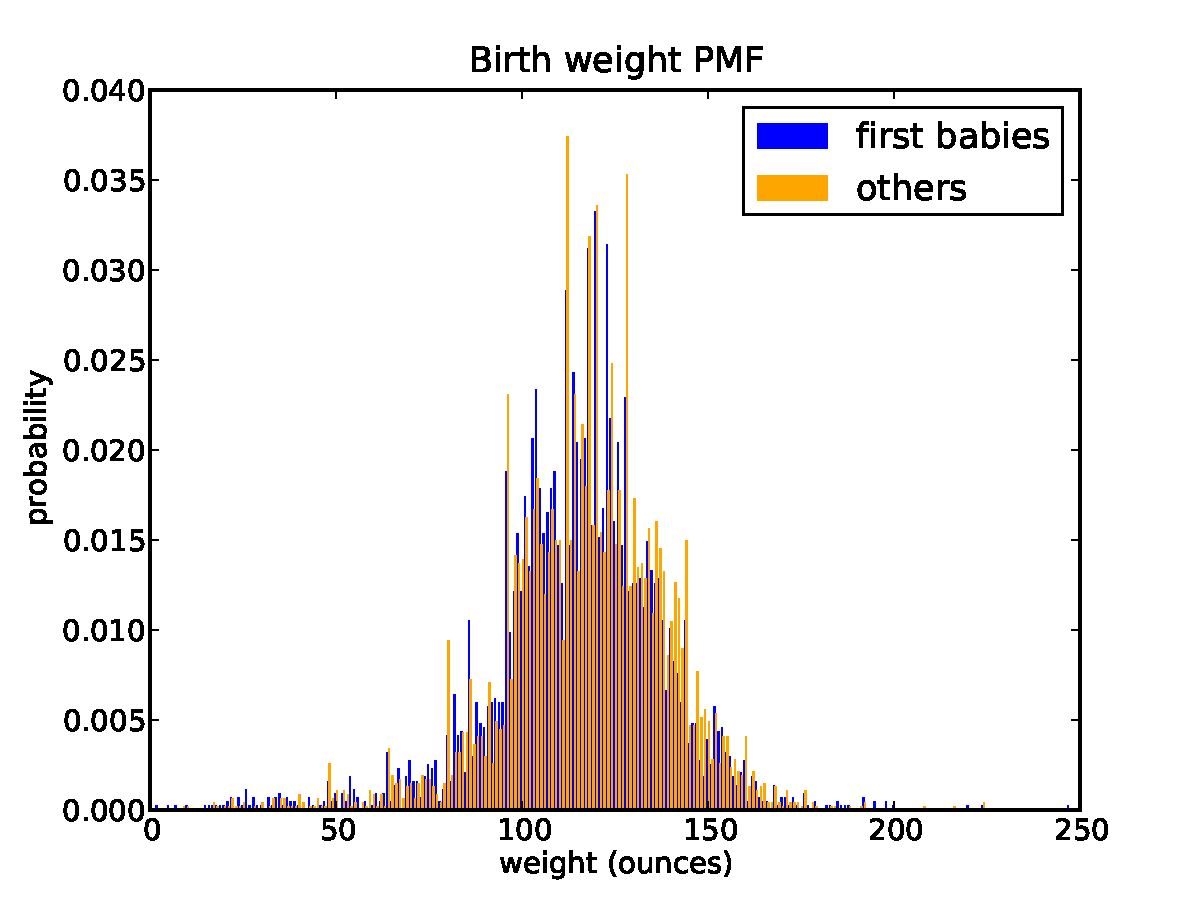
\includegraphics[height=2.5in]{figs/nsfg_birthwgt_pmf.pdf}}
\caption{PMF of birth weights.  This figure shows a limitation
of PMFs: they are hard to compare visually.}
\label{nsfg_birthwgt_pmf}
\end{figure}

전반적으로 분포는 정규분포의 종모양을 닮았다.
평균 근처에 값이 많고 체중이 더 높거나 더 낮아지면 값이 작아진다.

하지만 그림을 이해하기는 어렵다. 뾰족한 것과 골자기가 많고, 두 집단 분포 사이에
명백한 차이도 보인다. 여럿중에서 어느 면이 유의미한지 분간하기는 쉽지 않다.
또한 전반적인 패턴을 보기도 어렵다; 예를 들어, 여러분이 보기에 어느 분포가 평균값이 더 높은가?
\index{통에 담기(binning)}

데이터를 구간(bin)에 담는 것으로 이러한 문제는 완화될 수 있다; 즉, 값 범위를 서로 겹쳐지지 않는 구간으로 
나누고 각 구간(bin)에 값 갯수를 계수한다. 구간에 담는 것(binning)은 유용하지만,
적정한 구간 크기를 잡는 것은 까다롭다. 잡음을 평활(smooth out)하기 위해서 충분히 큰 통을 잡는 것이 
또한 유용한 정보도 평활할 수도 있다.

이러한 문제를 회피하는 대안이 누적분포함수(cumulative
distribution function, CDF)로 이번 장 학습주제다. 하지만, CDF를 설명하기 전에 백분위수(percentile)를 먼저 설명해야 한다.
\index{CDF}


\section{백분위수 (Percentiles)}
\index{백분위 순위 (percentile rank)}

만약 전국 단위 표준시험을 치르게 되면, 원점수와 {\bf 백분위 순위(percentile rank)} 형태로 시험결과를 받아보게 된다. 이러한 맥락에서 백분위 순위는 시험 당사자보다 적은 점수를 얻는 사람들이 된다.
그래서 만약 ``백분위수 90번째''라면, 시험을 치른 90\% 사람보다 혹은 동등하다는 의미가 된다.

다음에 {\tt scores} 시퀀스 값에서 상대적으로 \verb"your_score" 값에 대한 백분위 순위를 계산하는 방법이 있다.

%
\begin{verbatim}
def PercentileRank(scores, your_score):
    count = 0
    for score in scores:
        if score <= your_score:
            count += 1

    percentile_rank = 100.0 * count / len(scores)
    return percentile_rank
\end{verbatim}

예제로 만약 시퀀스 점수가 55, 66, 77, 88, 99이고, 시험 점수로 88점을 받았다면, 
백분위 순위는 {\tt 100 * 4 / 5}, 80이 된다.

값이 주어진다면, 백분위 순위를 찾기는 쉽다; 반대 방향으로는 다소 더 어렵다.
만약 백분위 순위가 주어진 상태에서 해당하는 값을 찾고자 한다면, 한 선택지는 값을 정렬하고
원하는 값을 찾는 것이다.

%
\begin{verbatim}
def Percentile(scores, percentile_rank):
    scores.sort()
    for score in scores:
        if PercentileRank(scores, score) >= percentile_rank:
            return score
\end{verbatim}

계산 결과는 {\bf 백분위수(percentile)}가 된다. 
예를 들어, 50번째 백분위 수는 백분위 순위가 50 인 값이 된다. 
시험점수 분포에서 50번째 백분위 수는 77이다.
\index{백분위수 (percentile)}

{\tt Percentile} 구현코드가 그다지 효율적이지 않다.
더 나은 접근법은 백분위 순위를 사용해서 해당하는 백분위수 인덱스를 계산하는 것이다.

\begin{verbatim}
def Percentile2(scores, percentile_rank):
    scores.sort()
    index = percentile_rank * (len(scores)-1) // 100
    return scores[index]
\end{verbatim}

``백분위수 (percentile)''와 ``백분위 순위 (percentile rank)'' 차이가 혼동스러울 수 있고
항상 용어를 정확하게 구별하여 사용하지는 않는다. 요약하면,
{\tt PercentileRank} 함수는 값을 인자로 받아 값 집합에서 백분위 순위를 계산한다;
{\tt Percentile} 함수는 백분위 순위를 인자로 받아 해당하는 값을 계산한다. 
\index{백분위 순위 (percentile rank)}

\section{CDF}
\index{CDF}

이제 백분위수와 백분위 순위를 이해하고 있기 때문에, {\bf 누적분포함수(cumulative distribution function, CDF)}를 다룰 준비가 되었다. CDF는 값을 백분위 순위로 매핑하는 함수다.
\index{누적분포함수 (cumulative distribution function)}
\index{백분위 순위 (percentile rank)}

CDF는 $x$의 함수로 $x$는 분포에 나타나는 임의값이다.  
특정한 $x$ 값에 대해서 $\CDF(x)$를 평가하기 위해서, 
$x$와 동일하거나 작은 분포의 분수값을 계산한다.

시퀀스 {\tt sample}와 값 {\tt x}를 인자로 받는 함수로 어떤 느낌인지 다음에 코드가 있다.

%
\begin{verbatim}
def EvalCdf(sample, x):
    count = 0.0
    for value in sample:
        if value <= x:
            count += 1

    prob = count / len(sample)
    return prob
\end{verbatim}

함수가 거의 {\tt PercentileRank}과 동일하지만, 백분위 순위가 0--100인 반면에 결과값이 0--1 범위를 갖는 확률이라는 점이 차이가 있다.
\index{표본 (sample)}

예제로 표본값으로 {\tt [1, 2, 2, 3, 5]}을 수집했다고 가정하자. 다음에 CDF로부터 값이 몇개 있다.
%
\[ CDF(0) = 0 \]
%
\[ CDF(1) = 0.2\]
%
\[ CDF(2) = 0.6\]
%
\[ CDF(3) = 0.8\]
%
\[ CDF(4) = 0.8\]
%
\[ CDF(5) = 1\]
%

표본에 있는 값뿐만 아니라 $x$의 임의값에 대해서 CDF를 평가할 수 있다.
만약 $x$가 표본에 가장 작은 값보다 작다면, $\CDF(x)$는 0.
만약 $x$가 가장 큰 값보다 크다면, $\CDF(x)$는 1.

\begin{figure}
% cumulative.py
%\centerline{\includegraphics[height=2.5in]{figs/cumulative_example_cdf.pdf}}
\caption{Example of a CDF.}
\label{example_cdf}
\end{figure}

그림~\ref{example_cdf}이 CDF를 그래픽으로 표현한 것이다.
표본 CDF는 계단 함수다.
\index{계단 함수 (step function)}


\section{CDF 표현하기 (Representing CDFs)}
\index{Cdf}

{\tt thinkstats2}은 CDF를 표현하는 Cdf라는 클래스를 제공한다. Cdf 가 제공하는 기본 메쏘드는 다음과 같다.

\begin{itemize}

\item {\tt Prob(x)}: {\tt x} 값이 주어졌을 때, $p = \CDF(x)$ 확률값을 계산한다. 꺾쇠 연산자는 {\tt Prob}와 동일하다.
\index{꺾쇠 연산자 (bracket operator)}

\item {\tt Value(p)}: 확률 {\tt p}가 주어졌을 때, 
상응하는 값 {\tt x}를 계산한다; 즉, {\tt p}의 {\bf CDF 역함수(inverse CDF)}다.
\index{CDF 역함수 (inverse CDF)}
\index{CDF, 역함수(inverse)}

\end{itemize}

\begin{figure}
% cumulative.py
%\centerline{\includegraphics[height=2.5in]{figs/cumulative_prglngth_cdf.pdf}}
\caption{CDF of pregnancy length.}
\label{cumulative_prglngth_cdf}
\end{figure}

Cdf 생성자는 인자로 리스트, 판다스 시리즈, Hist, Pmf, 혹은 또다른 Cdf를 받을 수 있다. NSFG 데이터에서 임신 기간 분포에 대한 Cdf를 생성하는 코드가 다음에 있다. 

\index{NSFG}
\index{임신 기간 (pregnancy length)}

\begin{verbatim}
    live, firsts, others = first.MakeFrames()
    cdf = thinkstats2.Cdf(live.prglngth, label='prglngth')
\end{verbatim}


{\tt thinkplot}은 {\tt Cdf}라는 함수를 제공해서 Cdf를 선그래프를 그릴 수 있다.
\index{thinkplot}

\begin{verbatim}
    thinkplot.Cdf(cdf)
    thinkplot.Show(xlabel='weeks', ylabel='CDF')
\end{verbatim}



그림~\ref{cumulative_prglngth_cdf}에 결과가 있다.
CDF를 읽는 한가지 방법은 백분위수를 찾는 것이다.
예를 들어, 임신 기간 10\%는 36주차보다 더 짧고, 90\%는 41주차보다 더 짧은 것처럼 보인다. 또는 CDF를 통해서 분포 모양을 시각적으로 표현할 수도 있다. 흔한 값은 CDF에서 급격하거나 수직적 부분으로 나타난다; 이번 예제에서 39주차 모드(최빈값)가 명확히 보인다. 30주차 밑으로 값이 몇개 없어서 이 범위에 있는 CDF는 평평하다.
\index{CDF, 해석하기 (interpreting)}

CDF에 익숙해지는데 시간이 좀 필요하다. 하지만, 한번 익숙해지면, PMF보다 더 많은 정보를 좀더 명확하게 보여줄 것으로 생각된다.


\section{CDF 비교하기}
\label{birth_weights}
\index{가족 성장 국가 조사 (National Survey of Family Growth)}
\index{NSFG}
\index{출산 체중 (birth weight)}
\index{체중 (weight)!출산 (birth)}

CDF는 특히 분포를 비교하는데 유용하다.
예를 들어, 첫째 아이와 첫째 아이가 아닌 아이에 대한 출산 체중 CDF를 플롯으로 그리는 코드가 다음에 있다.
\index{thinkplot}
\index{분포 (distributions), 비교하기 (comparing)}

\begin{verbatim}
    first_cdf = thinkstats2.Cdf(firsts.totalwgt_lb, label='first')
    other_cdf = thinkstats2.Cdf(others.totalwgt_lb, label='other')

    thinkplot.PrePlot(2)
    thinkplot.Cdfs([first_cdf, other_cdf])
    thinkplot.Show(xlabel='weight (pounds)', ylabel='CDF')
\end{verbatim}

\begin{figure}
% cumulative.py
%\centerline{\includegraphics[height=2.5in]{figs/cumulative_birthwgt_cdf.pdf}}
\caption{CDF of birth weights for first babies and others.}
\label{cumulative_birthwgt_cdf}
\end{figure}

그림~\ref{cumulative_birthwgt_cdf}에 결과가 있다.
그림~\ref{nsfg_birthwgt_pmf}와 비교하여, 좀더 명확하게 분포 모양과 분포간의 차이를 그림에서 보여준다.
첫째 아이 체중이 평균 이상에서 조금더 커다란 불일치성을 보이고, 분포 전반에 걸쳐 다소 가볍다는 것을 볼 수 있다.

\index{모양 (shape)}

\section{백분위수 기반 통계량 (Percentile-based statistics)}
\index{요약 통계 (summary statistic)}
\index{사분위수 범위 (interquartile range)}
\index{분위수 (quartile)}
\index{백분위수 (percentile)}
\index{중위수 (median)}
\index{중심 경향성 (central tendency)}
\index{퍼짐 (spread)}

CDF를 계산하게 되면, 백분위수와 백분위 순위를 계산하기는 쉽다.
Cdf 클래스가 두가지 메쏘드를 제공한다.
\index{Cdf}
\index{백분위 순위 (percentile rank)}

\begin{itemize}

\item {\tt PercentileRank(x)}: {\tt x}가 주어지면, $100 \cdot \CDF(x)$ 백분위 순위를 계산한다.

\item {\tt Percentile(p)}: 백분위 순위 {\tt rank}가 주어지면,
해당하는 값 {\tt x}를 계산한다. {\tt Value(p/100)}과 동등하다.

\end{itemize}

{\tt 백분위수 (Percentile)}는 백분위수 기반 요양 통계량을 계산하는데 사용될 수 있다. 예를 들어 50번째 백분위수는 {\bf 중위수 (median)}로 알려진 분포를 반으로 나누는 값이다. 평균과 마찬가지로 중위수는 분포의 중심경향성을 측정하는 측도다.

사실, 각기 다른 특성을 가진 ``중위수(median)''에 대한 정의가 몇개 있다. 하지만, {\tt Percentile(50)}가 단순하고 계산하기 효율적이다.

또 다른 백분위수 기반 통계량이 {\bf 사분위수 범위 (interquartile range, IQR}로 분포의 퍼짐을 측정하는 측도다.
IQR는 75번째와 25번째 백분위수 간의 차이다.

좀더 일반적으로, 백분위수는 종종 분포 모양을 요약하는데 쓰여진다.
예를 들어, 수입 분포는 종종 ``분위수 (quintiles)''로 보고된다; 즉, 20번째, 40번째, 60번째, 80번째 백분위수로 쪼개진다.
다른 분포는 10개 ``십분위(deciles)''으로 나눠진다.
이와 같이 CDF에서 동일간격으로 표현되는 통계량을 {\bf 분위수(quantiles)}라고 한다. 좀더 자세한 정보는 다음 웹사이트를 참고 바란다. \url{https://en.wikipedia.org/wiki/Quantile}.
\index{분위수 (quantile)}
\index{오분위수 (quintile)}
\index{십분위수 (decile)}


\section{난수 (Random numbers)}
\label{random}
\index{난수 (random number)}

정상 출산 모집단에서 임의 표본을 추출하고, 출생 체중 백분위 순위를 찾아낸다고 가정하자. 이제 백분위 순위 CDF를 계산한다고 가정하자.
분포가 어떨 것으로 생각하는가?

\index{백분위 순위 (percentile rank)}
\index{출생 체중 (birth weight)}
\index{체중 (weight)!출생 (birth)}

다음에 어떻게 계산하는지 코드가 있다. 첫째로 출생 체중 Cdf를 생성한다.
\index{Cdf}

\begin{verbatim}
    weights = live.totalwgt_lb
    cdf = thinkstats2.Cdf(weights, label='totalwgt_lb')
\end{verbatim}

그리고 나서, 표본을 생성하고, 표본에 있는 각 값에 대한 백분위 순위를 계산한다.

\begin{verbatim}
    sample = np.random.choice(weights, 100, replace=True)
    ranks = [cdf.PercentileRank(x) for x in sample]
\end{verbatim}

{\tt sample}은 100개 출생 체중 임의 표본이며 복원 추출하였다;
즉, 동일한 값이 한번이상 추출될 수 있다. 
{\tt ranks}는 백분위 순위 리스트다.
\index{복원 (replacement)}

마지막으로 백분위 순위 Cdf를 만들고 플롯으로 그린다.

\index{thinkplot}

\begin{verbatim}
    rank_cdf = thinkstats2.Cdf(ranks)
    thinkplot.Cdf(rank_cdf)
    thinkplot.Show(xlabel='percentile rank', ylabel='CDF')
\end{verbatim}

\begin{figure}
% cumulative.py
%\centerline{\includegraphics[height=2.5in]{figs/cumulative_random.pdf}}
\caption{CDF of percentile ranks for a random sample of birth weights.}
\label{cumulative_random}
\end{figure}

그림~\ref{cumulative_random}이 결과를 보여준다.
CDF가 근사적으로 직선이다. 분포가 균등하다라는 의미다. 

결과가 명확하지 않을 수도 있지만, CDF가 정의된 방식의 결과다.
그림이 보여주는 정보는 표본의 10\%가 10번째 백분위수 보다 밑에 있고,
표본의 20\%가 20번째 백분위수 보다 밑에 있고 등등, 정확히 예측했던 것이다.

그래서, CDF 모양에 관계없이, 백분위 순위 분포는 균등하다. 
이 속성이 유용한데, 이유는 주어진 CDF에서 난수를 생성하는데 있어서 간단하면서도 효율적인 알고리즘 설계하는 기초가 되기 때문이다; 다음에 난수를 생성하는 방법이 있다.

\index{역 CDF 알고리즘 (inverse CDF algorithm)}
\index{난수 (random number)}

\begin{itemize}

\item 0--100 범우에서 균등하게 백분위 순위를 고른다.

\item {\tt Cdf.Percentile}를 사용해서 선택한 백분위 순위에 상응하는 값을 분포에서 찾는다.
\index{Cdf}

\end{itemize}

Cdf는 상기 알고리즘을 구현한 것으로 {\tt Random}이 함수명이다.

\begin{verbatim}
# class Cdf:
    def Random(self):
        return self.Percentile(random.uniform(0, 100))
\end{verbatim}

Cdf는 {\tt Sample} 메쏘드를 제공하는데 정수 {\tt n}을
인자로 받아 Cdf에서 임의로 추출한 {\tt n}개 리스트를 반환한다.


\section{백분위 순위 비교하기}

백분위 순위는 다른 집단에 대해서 측정값을 비교하는데 유용하다.
예를 들어, 달리기 경주에서 참가자는 대체로 나이와 성별로 무리를 만든다.
다른 연령 집단에 있는 사람을 비교하는데 경주시간을 백분위 순위로 변환할 수 있다.

\index{백분위 순위 (percentile rank)}

몇년전에 매사추세츠(Massachusetts)주에서 제임스 조이스(James Joyce) 10킬로 마라톤을 뛰었다;
42분 44초로 주파해서 1633명중에서 97번째로 완주했다. 참가자 1633명 중 1537명 참가자보다 빨리 도착해서 
저자의 최종 백분위 순위는 94\%다.  
\index{제임스 조이스 마라톤 (James Joyce Ramble} 
\index{경주 시간 (race time)}


좀더 일반적으로, 위치와 필드 크기 정보가 주어진다면, 백분위 순위를 계산할 수 있다.
\index{필드 크기 (field size)}

\begin{verbatim}
def PositionToPercentile(position, field_size):
    beat = field_size - position + 1
    percentile = 100.0 * beat / field_size
    return percentile
\end{verbatim}

``40에서 49세 남성'', M4049로 표기된 저자가 속한 연령집단, 256명 중에서 26번째로 완주했다.
그래서, 저자가 속한 연령집단에서 백분위 순위는 90\%가 된다.
\index{연령 집단 (age group)}

10년정도 더 마라톤을 뛴다면 (그리고 계속해서 뛰고 싶다.), M5059 그룹에 있을 것이다.
저자가 속한 집단에서 동일한 백분위수를 유지한다고 가정한다면, 완주하는데 얼마나 더 시간이 필요할까?

M4049 집단에 있는 저자의 백분위 순위를 M5059 집단에 위치로 전환하면 상기 질문에 대답할 수 있다.
다음에 프로그램 코드가 있다.

\begin{verbatim}
def PercentileToPosition(percentile, field_size):
    beat = percentile * field_size / 100.0
    position = field_size - beat + 1
    return position
\end{verbatim}

M5059 집단에 171 명이 있어서 동일한 백분위 순위를 유지하려면 17번째와 18번째 사이에서 완주해야 한다.
M5059에서 17번째 마라토너가 46:05로 완주해서, 40대 동일한 백분위 순위를 유지하는데 
46:05 시간이 완주 목표시간이 된다.


\section{Exercises}

For the following exercises, you can start with \verb"chap04ex.ipynb".
My solution is in \verb"chap04soln.ipynb".

\begin{exercise}
How much did you weigh at birth?  If you don't know, call your mother
or someone else who knows.  Using the NSFG data (all live births),
compute the distribution of birth weights and use it to find your
percentile rank.  If you were a first baby, find your percentile rank
in the distribution for first babies.  Otherwise use the distribution
for others.  If you are in the 90th percentile or higher, call your
mother back and apologize.
\index{birth weight}
\index{weight!birth}

\end{exercise}

\begin{exercise}
The numbers generated by {\tt random.random} are supposed to be
uniform between 0 and 1; that is, every value in the range
should have the same probability.

Generate 1000 numbers from {\tt random.random} and plot their
PMF and CDF.  Is the distribution uniform?
\index{uniform distribution}
\index{distribution!uniform}
\index{random number}

\end{exercise}


\section{용어사전}

\begin{itemize}

\item 백분위 순위 (percentile rank): 
분포에서 주어진 값과 동일하거나 적은 값의 퍼센티지.
\index{백분위 순위 (percentile rank)}

\item 백분위수 (percentile): 주어진 백분위 순위와 연관된 값.
\index{백분위수 (percentile)}

\item 누적분포함수 (cumulative distribution function, CDF): 
값에서 누적확률값으로 매핑하는 함수. $\CDF(x)$는 $x$와 동일하거나 작은 표본비율이다. 
\index{CDF}
\index{누적 확률 (cumulative probability)}

\item 역 CDF (inverse CDF):
누적 확률($p$)에서 해당값으로 매핑하는 함수.
\index{역 CDF (inverse CDF)}
\index{CDF, 역 (inverse)}

\item 중위수 (median): 
종종 중심경향성 측도로 사용되는 50번째 백분위수.
\index{중위수 (median)}

\item 사분위 범위 (interquartile range): 
퍼짐의 측도로 사용되는 75번째와 25번째 백분위수 간 차이.
\index{사분위 범위 (interquartile range)}

\item 분위수 (quantile): 
동일 간격 백분위 순위에 상응하는 스퀀스 값; 예를 들어, 
분포 사분위수는 25번째, 50번째, 75번째 백분위수가 된다.
\index{분위수 (quantile)}

\item 복원 (replacement): 
표본추출 과정의 속성. ``복원추출 (With replacement)''는 동일한 값이 한번이상 추출될 수 있다는 의미다;
``비복원추출 (Without replacement)''는 값이 한번 추출될면, 모집단에서 제거된다는 의미가 된다.
\index{복원 (replacement)}

\end{itemize}


\chapter{분포 모형화 (Modeling distributions)}
\label{modeling}

지금까지 사용한 분포는 {\bf 경험적 분포 (empirical distributions)}라고 부른다.
이유는 필연적으로 유한 표본인 경험적 관측치에 기반하고 있기 때문이다.

\index{해석 분포 (analytic distribution)}
\index{분포 (distribution)!해석 (analytic)}
\index{경험적 분포 (empirical distribution)}
\index{분포 (distribution)!경험 (empirical)}

수학 함수인 CDF로 특징 지어지는 {\bf 해석 분포 (analytic distribution)}가 대안이 된다.
해석 분포가 경험적 분포를 모형화하는데 사용될 수 있다.
이러한 맥락에서 {\bf 모형(model)}은 불필요한 부분을 덜어낸 단순화가 된다.
이번 장에서 자주 사용되는 분포를 제시하고 이를 사용하여 다양한 출처를 가진 
데이터를 모형화한다.

\index{모형 (model)}

이번 장에서 사용되는 코드는 {\tt analytic.py}에 있다.
코드를 다운로드하고 작업하는 것에 대한 정보는 ~\ref{code}을 참조한다.


\section{지수분포 (exponential distribution)}
\label{exponential}
\index{지수분포 (exponential distribution)}
\index{분포 (distribution)!지수 (exponential)}

\begin{figure}
% analytic.py
%\centerline{\includegraphics[height=2.5in]{figs/analytic_expo_cdf.pdf}}
\caption{CDFs of exponential distributions with various parameters.}
\label{analytic_expo_cdf}
\end{figure}

{\bf 지수 분포 (exponential distribution)}로 시작하는데 이유는 상대적으로 단순하기 때문이다.
지수분포 CDF는 다음과 같다.
%
\[ \CDF(x) = 1 - e^{-\lambda x} \]
%

모수 $\lambda$가 분포 형상(shape)을 결정한다. 
그림~\ref{analytic_expo_cdf}에서 $\lambda = $ 0.5, 1, 2 값을 가진
CDF가 대략 모양이 어떤지 볼 수 있다.
\index{모수 (parameter)}

현실 세계에서 일련의 사건을 보고, 사건 간에 시간({\bf 도착간격 시간, interarrival times})을 측정할 때 지수분포가 등장한다.
만약 사건이 언제든지 균등하게 발생할 것 같다면 도착간격 시간 분포는 지수분포같은 경향이 있다.
\index{도착간격 시간 (interarrival time)}

일례로, 출생간 발생시간을 살펴보자. 1997년 12월 18일 호주 브리즈번
\footnote{예제에 나오는 자료와 정보는 저널 논문에 기반한다. Dunn, ``A Simple Dataset for Demonstrating Common Distributions,'' Journal of Statistics Education v.7, n.3 (1999)}
에서 44명 신생아가 출생했다. 모든 44명 신생아 출생 시간이 지역신문에 출간되었다;
전체 데이터셋은 {\tt ThinkStats2} 저장소 {\tt babyboom.dat} 파일에 담겨있다.
\index{출생 시간 (birth time)}
\index{호주 (Australia)} 
\index{브리즈번 (Brisbane)}

\begin{verbatim}
    df = ReadBabyBoom()
    diffs = df.minutes.diff()
    cdf = thinkstats2.Cdf(diffs, label='actual')

    thinkplot.Cdf(cdf)
    thinkplot.Show(xlabel='minutes', ylabel='CDF')
\end{verbatim}

{\tt ReadBabyBoom} 함수가 데이터 파일을 읽어들이고 {\tt time}, {\tt sex}, \verb"weight_g", {\tt minutes}
칼럼으로 구성된 데이터프레임을 반환한다.
여기서 {\tt minutes}가 자정 이후 출생시간을 분으로 변환한 시간정보를 담고 있다.
\index{데이터프레임 (DataFrame)}
\index{thinkplot}

\begin{figure}
% analytic.py
%\centerline{\includegraphics[height=2.5in]{figs/analytic_interarrivals.pdf}}
\caption{CDF of interarrival times (left) and CCDF on a log-y scale (right).}
\label{analytic_interarrival_cdf}
\end{figure}

%\begin{figure}
% analytic.py
%%\centerline{\includegraphics[height=2.5in]{figs/analytic_interarrivals_logy.pdf}}
%\caption{CCDF of interarrival times.}
%\label{analytic_interarrival_ccdf}
%\end{figure}

{\tt diffs}는 연속되는 출생시간 사이 차이가 되고 
{\tt cdf}는 출생간격 시간 분포가 된다.
그림~\ref{analytic_interarrival_cdf} (왼편)이 CDF를 나타낸다.
전형적인 지수분포 형상을 지닌 처럼 보이지만, 어떻게 분간할 수 있을까?

한 방법은 {\bf 보완 CDF (complementary CDF)}를 플롯으로 그리는 것이다.
보완 CDF는 log-y 척도로 $1 - \CDF(x)$이다.
지수분포 데이터에 대해서는 결과가 직선이다. 왜 그런지 살펴보자.

\index{보완 CDF (complementary CDF)} 
\index{CDF!보완 (complementary)} 
\index{CCDF}

독자가 생각하기에 지수분포를 따르는 데이터셋을 보완 CDF(CCDF) 플롯으로 그리면, 
다음과 같은 함수가 나올 것으로 기대한다.
%
\[ y \approx e^{-\lambda x} \]
%
양변에 로그를 취하면 다음과 같다.
%
\[ \log y \approx -\lambda x\]
%
그래서, log-y 척도로 CCDF는 기울기 $-\lambda$인 직선이 된다.
다음에 플롯을 생성하는 방법이 있다.
\index{로그 척도 (logarithmic scale)}
\index{보완 CDF (complementary CDF)}
\index{CDF!보완 (complementary)}
\index{CCDF}

\begin{verbatim}
    thinkplot.Cdf(cdf, complement=True)
    thinkplot.Show(xlabel='minutes',
                   ylabel='CCDF',
                   yscale='log')
\end{verbatim}

{\tt complement=True} 인자가 있어서, {\tt thinkplot.Cdf}이 플롯을 그리기 전에
보완 CDF를 계산한다. 그리고 {\tt yscale='log'}를 통해서  
{\tt thinkplot.Show}가 로그 척도로 {\tt y}축을 고정한다.
\index{thinkplot}
\index{Cdf}

그림~\ref{analytic_interarrival_cdf} (오른편)에 결과가 있다.
정확하게 직선이 아니다. 이 데이터에 대해서 완벽한 모델로 지수 분포가 아니라는 것이 표시된다.
기본 가정---출생이 아무 때고 균등하게 발생---이 정확하게 사실이 아닐 것이다.
그럼에도 불구하고 지수분포로 이 데이터셋을 모형화하는 것이 합리적일 것이다.
이와 같은 단순화로 단 하나의 모수로 분포를 요약할 수 있다.
\index{모형 (model)}

모수 $\lambda$가 율(rate)로 해석될 수 있다; 즉, 평균적으로 단위 시간에 
발생하는 사건 수. 예제에서 44명의 신생아가 24시간내에 태어난다.
그래서 율값이 분당 $\lambda = 0.0306$이 된다.
지수분포 평균은 $1/\lambda$ 으로 신생아 간에 출생 평균 시간은 32.7분이 된다.

\section{정규 분포 (normal distribution)}
\label{normal}

가우스 분포(Gaussian distribution)라고도 불리는 
{\bf 정규 분포 (normal distribution)}가 흔히 사용되는데 이유는 많은 현상을 기술하고 
최소한 근사적으로도 기술할 수 있기 때문이다.
\ref{CLT} 절에서 다루게 되는데 이와 같은 보편성에는 이유가 있다.
\index{CDF}
\index{모수 (parameter)}
\index{평균 (mean)}
\index{표준편차 (standard deviation)}
\index{정규 분포 (normal distribution)}
\index{분포 (distribution)!정규 (normal)}
\index{가우스 분포 (Gaussian distribution)}
\index{분포 (distribution)!가우스 (Gaussian)}

%
\[ \CDF(z) = \frac{1}{\sqrt{2 \pi}} \int_{-\infty}^z e^{-t^2/2} dt \]
%

\begin{figure}
% analytic.py
%\centerline{\includegraphics[height=2.5in]{figs/analytic_gaussian_cdf.pdf}}
\caption{CDF of normal distributions with a range of parameters.}
\label{analytic_gaussian_cdf}
\end{figure}

정규 분포는 모수 두개로 특성화된다: 평균 $\mu$, 표준편차 $\sigma$.
모수 $\mu=0$과 $\sigma=1$을 갖는 정규분포를 {\bf 표준 정규 분포 (standard normal
 distribution)}라고 한다.
정규분포 CDF는 닫힌 형식 해법(closed form solution)을 갖지 않는 적분으로 정의된다.
하지만, 효율적으로 계산하는 알고리즘이 있다.
알고리즘 중 하나가 SciPy을 통해 제공된다: {\tt scipy.stats.norm}이
정규분포를 표현하는 객체다. 표준 정규분포 CDF를 계산하는 {\tt cdf} 메쏘드를 제공한다.

\index{SciPy}
\index{닫힌 형식 (closed form)}

\begin{verbatim}
>>> import scipy.stats
>>> scipy.stats.norm.cdf(0)
0.5
\end{verbatim}

결과값은 맞다: 표준 정규분포 중위수는 0 (평균과 같다)이고, 값의 절반이 중위수 아래 위치한다.
그래서 $\CDF(0)$은 0.5 이다.

{\tt norm.cdf}은 옵션 모수를 받는다: {\tt loc}가
평균을 특정하고, {\tt scale}는 표준편차를 특정한다.


{\tt thinkstats2}는 상기 함수를 좀더 사용하기 쉽게 한다.
{\tt EvalNormalCdf} 메쏘드는 {\tt mu}과 {\tt sigma}을 인자로 받아 
{\tt x}에 CDF를 계산한다.

\index{정규 분포 (normal distribution)}

\begin{verbatim}
def EvalNormalCdf(x, mu=0, sigma=1):
    return scipy.stats.norm.cdf(x, loc=mu, scale=sigma)
\end{verbatim}

그림~\ref{analytic_gaussian_cdf}에 정규분포에 다양한 모수를 넣어 그린 CDF가 있다.
곡선의 S자(sigmoid) 형상이 정규분포를 식별할 수 있게 하는 특성이다.

앞장에서 NSFG 출생 체중 분포를 살펴봤다.
모든 정상 출산 체중에 대한 경험적 CDF와 동일한 평균과 분산으로 정규분포 CDF를 중첩하여 
플롯으로 그린 것이 그림~\ref{analytic_birthwgt_model}이다.

\index{가족 성장 국가 조사 (National Survey of Family Growth)}
\index{NSFG}
\index{출생 체중 (birth weight)}
\index{체중 (weight)!출생 (birth)}

\begin{figure}
% analytic.py
%\centerline{\includegraphics[height=2.5in]{figs/analytic_birthwgt_model.pdf}}
\caption{CDF of birth weights with a normal model.}
\label{analytic_birthwgt_model}
\end{figure}

정규분포가 이 데이터셋에 대해서 좋은 모형이 된다.
그래서 만약 모수 $\mu = 7.28$과 $\sigma = 1.24$으로 
분포를 요약한다면, 결과 오차(모형과 데이터 간 차이)가 작다.

\index{모형 (model)}
\index{백분위수 (percentile)}

백분위수 10번째 아래에서 데이터와 모형 사이에 불일치가 있다.
정규분포에서 예측되는 것보다 더 많이 체중이 적은 아이가 있다.
만약 조산아에 특별히 관심이 있다면, 분포에서 이 부분을 잘 적합하는 것이 중요하다.
그래서 정규분포를 사용하는 것이 적절하지 않을 수도 있다.


\section{정규확률그림 (Normal probability plot)}

지수분포와 몇가지 분포에서 대해서 해석분포(analytic distribution)가 특정 데이터셋에 대해서
적합한 모형인가를 테스트하는데 사용할 수 있는 간단한 변환이 있다.

\index{지수분포 (exponential distribution)}
\index{분포 (distribution)!지수 (exponential)}
\index{모형 (model)}

정규분포에 대해서 그러한 변환은 없다. 하지만, 
{\bf 정규확률그림 (normal probability plot)}으로 불리는 대안이 있다.
정규확률그림을 생성하는 방식이 두개 있다.: 어려운 방식과 쉬운 방식.
어려운 방식에 관심이 있다면 \url{https://en.wikipedia.org/wiki/Normal_probability_plot}에서 
자세한 정보를 얻을 수 있다.
다음에 쉬운 방식이 있다.
\index{정규확률그림 (normal probability plot)}
\index{그림 (plot)! 정규확률 (normal probability)}
\index{정규분포 (normal distribution)}
\index{분포 (distribution)!정규 (normal)}
\index{가우스 분포 (Gaussian distribution)}
\index{분포 (distribution)!가우스 (Gaussian)}

\begin{enumerate}

\item 표본에 있는 값을 정렬한다.

\item 표준정규분포($\mu=0$, $\sigma=1$)에서 표본과 동일한 크기를 갖는 난수을 생성하고
정렬한다.
\index{난수 (random number)}

\item 표본에서 나온 정렬된 값과 난수를 플롯으로 그린다.

\end{enumerate}

만약 표본 분포가 근사적으로 정규분포라면, 결과는 
절편 {\tt mu}, 기울기 {\tt sigma}를 갖는 직선이다.
{\tt thinkstats2}에 {\tt NormalProbability}이 있다.
표본을 인자로 받아서 넘파이(NumPy) 배열 두개를 반환한다.
\index{넘파이 (NumPy)}

\begin{verbatim}
xs, ys = thinkstats2.NormalProbability(sample)
\end{verbatim}

\begin{figure}
% analytic.py
%\centerline{\includegraphics[height=2.5in]{figs/analytic_normal_prob_example.pdf}}
\caption{Normal probability plot for random samples from normal distributions.}
\label{analytic_normal_prob_example}
\end{figure}

{\tt ys}는 {\tt sample}에서 정렬된 값이 담겨있다; 
{\tt xs}에는 표준정규분포에서 생성된 난수가 담겨있다.

{\tt NormalProbability}을 테스트하기 위해서 다양한 모수를 가진 
정규분포에서 모조 샘플을 생성했다.
그림~\ref{analytic_normal_prob_example}에 결과가 있다.
선들이 근사적으로 직선으로, 평균에 있는 값보다 벗어난 값을 꼬리에 갖는다.

이제 실제 데이터에 적합을 시도해 보자.
앞절로부터 출생 체중 데이터에 대해 정규확률그림을 생성하는 코드가 다음에 있다.
모형을 표현하는 회색선과 실제 데이터를 표현하는 파란선을 플롯으로 그린다.

\index{출생 체중 (birth weight)}
\index{체중 (weight)!출생 (birth)}

\begin{verbatim}
def MakeNormalPlot(weights):
    mean = weights.mean()
    std = weights.std()

    xs = [-4, 4]
    fxs, fys = thinkstats2.FitLine(xs, inter=mean, slope=std)
    thinkplot.Plot(fxs, fys, color='gray', label='model')

    xs, ys = thinkstats2.NormalProbability(weights)
    thinkplot.Plot(xs, ys, label='birth weights')
\end{verbatim}

{\tt weights}는 출생 체중 판다스 시리즈다; {\tt mean}과 {\tt std}은
각각 평균과 표준편차다.
\index{판다스 (pandas)}
\index{시리즈 (Series)}
\index{thinkplot}
\index{표준편차 (standard deviation)}

{\tt FitLine}이 시퀀스 {\tt xs}, 절편, 기울기를 인자로 받는다;
반환하는 {\tt xs}와 {\tt ys}는 {\tt xs} 값에서 계산되어 인자로 받은 모수를 가진 직선이다.

{\tt NormalProbability}은 {\tt xs}와 {\tt ys}를 반환하는데 
표준정규분포에서 나온 값과 {\tt weights}에서 나온 값을 담고 있다.
만약 체중 분포가 정규분포를 따른다면, 데이터도 모델과 매칭되어야 한다.

\index{모형 (model)}

\begin{figure}
% analytic.py
%\centerline{\includegraphics[height=2.5in]{figs/analytic_birthwgt_normal.pdf}}
\caption{Normal probability plot of birth weights.}
\label{analytic_birthwgt_normal}
\end{figure}

그림~\ref{analytic_birthwgt_normal}이 전체 정상 출생과 더불어 만삭(임신기간이 36주 이상)에 대한 결과를 보여준다.
두 곡선 모두 평균 근처에서 모형과 매칭되고 꼬리에서 차이가 난다.
가장 무거운 아이가 모형이 예측한 것보다 더 무겁고, 가장 가벼운 아이는 더 가볍다.

\index{임신 기간}

단지 만삭 아이만 선택해서, 가장 가벼운 몇몇 아이를 제거하면 분포 아래쪽 꼬리에 있는 불일치를 줄일 수 있다.

정규분포 모형이 평균에서부터 몇 표준편차 내에서 분포를 잘 기술하지만, 꼬리 부근에서는 아니라고 플롯 그래프를 통해서 알 수 있다.
실제 목적에 얼마나 부합되는지는 목적에 달려있다.
\index{모형 (model)}
\index{출생 체중 (birth weight)}
\index{체중 (weight)!출생 (birth)}
\index{표준편차 (standard deviation)}


\section{로그 정규분포 (lognormal distribution)}
\label{brfss}
\label{lognormal}

만약 값을 로그 취한 집합이 정규분포라면, 이 값은 {\bf 로그 정규분포 (lognormal distribution)}다. 로그 정규분포 CDF는 $x$를 $\log x$로 치환한 정규분포 CDF와 동일하다.
%
\[ CDF_{lognormal}(x) = CDF_{normal}(\log x)\]
%
로그 정규분포 모수는 일반적으로 $\mu$와 $\sigma$로 표기한다.
하지만, 기억할 것은 모수가 평균과 표준편차는 {\em 아니다};
로그 정규분포 평균은 $\exp(\mu +\sigma^2/2)$이고, 표준편차는 조금 복잡한다.(\url{http://wikipedia.org/wiki/Log-normal_distribution}를 참조한다)
\index{모수 (parameter)} 
\index{체중 (weight)!성인 (adult)} 
\index{성인 체중 (adult weight)}
\index{로그 정규분포 (lognormal distribution)}
\index{분포 (distribution)!로그 정규 (lognormal)}
\index{CDF}

\begin{figure}
% brfss.py
%\centerline{
%\includegraphics[height=2.5in]{figs/brfss_weight.pdf}}
%\caption{CDF of adult weights on a linear scale (left) and
%log scale (right).}
%\label{brfss_weight}
\end{figure}

만약 표본이 근사적으로 로그 정규분포이고 log-x 척도로 CDF 플롯을 그린다면, 정규분포 특성의 형상을 갖는다.
표본이 로그 정규분포 모형과 얼마나 잘 적합하는지 테스트하기 위해서, 
표본값에 로그를 취해서 정규확률그림을 생성할 수 있다.

\index{정규확률그림 (normal probability plot)}
\index{모형 (model)}

예제로 성인 체중 분포를 살펴보는데 근사적으로 로그 정규분포다.\footnote{\url{http://mathworld.wolfram.com/LogNormalDistribution.html} 사이트에서 주석(인용없이)으로 이 가능성에 대해서 제보를 받았다.
나중에 로그 변환과 원인을 제안하는 논문을 발견했다: Penman and Johnson, ``The Changing Shape of the Body Mass Index Distribution Curve in the Population,'' Preventing Chronic Disease, 2006 July; 3(3): A74.  Online at \url{http://www.ncbi.nlm.nih.gov/pmc/articles/PMC1636707}.}


만성 질환 예방 및 건강 증진을 위한 국립 센터 (National Center for Chronic Disease Prevention and Health Promotion)에서는 
행동 위험 요인 감시 시스템(Behavioral Risk Factor Surveillance System, BRFSS)\footnote{질병통제 예방센터(Centers for Disease Control and Prevention, CDC). 행동 위험 요인 감시 시스템 조사 자료(Behavioral Risk Factor Surveillance System Survey Data). Atlanta, Georgia: 미국 보건 복지부 (U.S. Department of Health and Human Services), 질병통제 예방센터 (Centers for Disease Control and Prevention), 2008.}의 일부문으로 매년 조사를 실시한다.
2008년 414,509 응답자를 대상으로 인터뷰했고 인구통계, 건강, 건강 위험에 관해서 설문했다. 수집한 데이터 중에 398,484 응답자 킬로그램으로 표시된 체중정보가 있다.
\index{행동 위험 요인 감시 시스템 (Behavioral Risk Factor Surveillance System)}
\index{BRFSS}

이 책을 위한 저장소에 BRFSS에 관한 데이터를 담고 있는 고정폭 아스키(ASCII)파일, {\tt CDBRFS08.ASC.gz}와 더불어 파일을 읽고 데이터를 분석하는 {\tt brfss.py}파일도 함께 있다.

\begin{figure}
% brfss.py
%\centerline{
%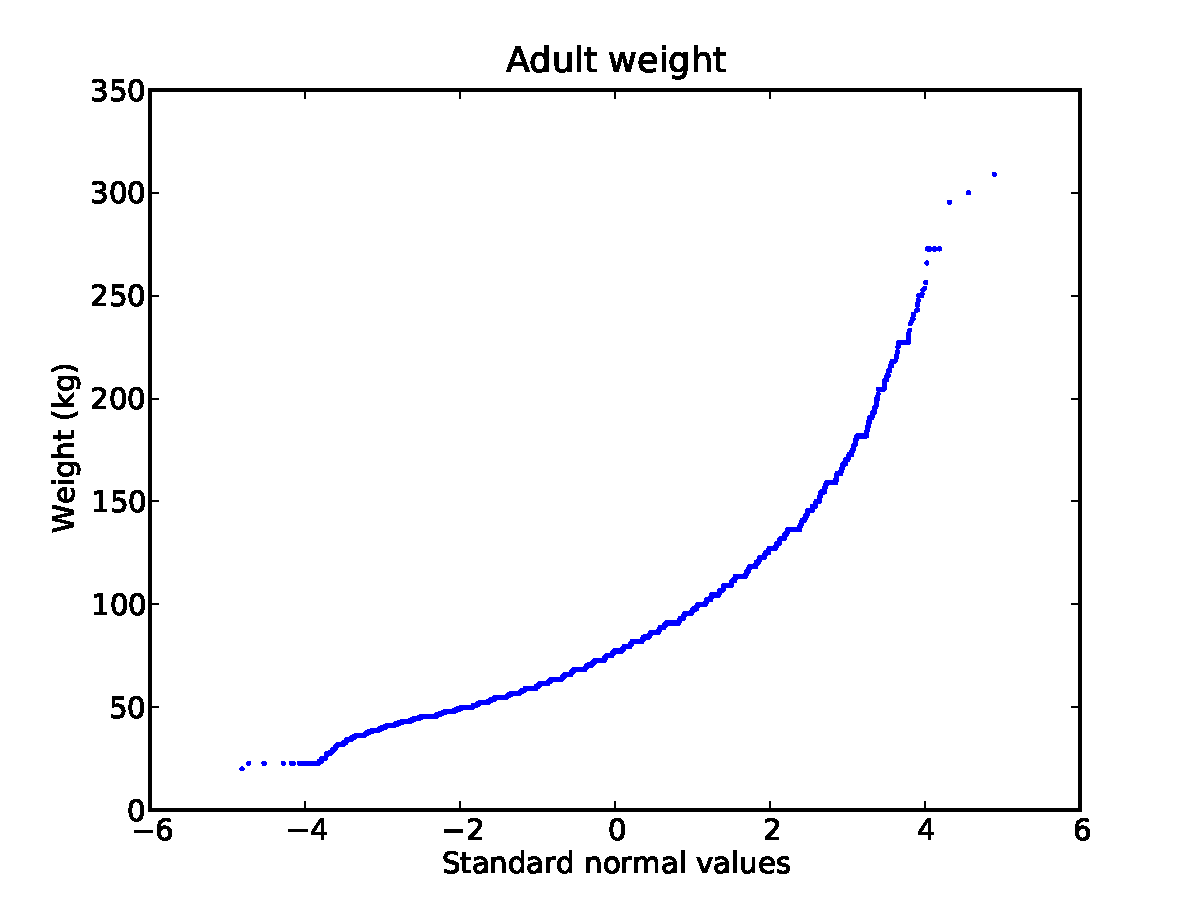
\includegraphics[height=2.5in]{figs/brfss_weight_normal.pdf}}
\caption{Normal probability plots for adult weight on a linear scale
  (left) and log scale (right).}
\label{brfss_weight_normal}
\end{figure}

그림~\ref{brfss_weight} (왼편)이 정규분포 모형에 선형 척도로 성인 체중 분포를 나타낸다.
그림~\ref{brfss_weight} (오른편)이 로그 정규분포 모형으로 로그 척도로 동일한 분포를 나타낸다.
로그 정규 모형이 더 나은 적합이지만 데이터를 이와 같이 표현하는 것이 차이점을 특별히 인상적으로 만들지는 못한다.
\index{응답자 (respondent)} 
\index{모형 (model)}

그림~\ref{brfss_weight_normal}이 성인 체중 $w$에 대한 정규확률그림과 
로그 변환한 체중 $\log_{10} w$에 대한 정규확률그림을 보여준다.
이제 데이터가 정규분포 모형에서 상당히 벗아난 것이 명확하다.
다른 한편으로 로그 정규모형은 데이터에 대한 좋은 매칭을 보여준다.

\index{정규분포 (normal distribution)} 
\index{분포 (distribution)!정규 (normal0}
\index{가우스 분포 (Gaussian distribution)} 
\index{분포 (distribution)!가우스 (Gaussian)}
\index{로그 정규분포 (lognormal distribution)} 
\index{분포 (distribution)!로그 정규 (lognormal)}
\index{표준편차 (standard deviation)} 
\index{성인 체중 (adult weight)} 
\index{체중 (weight)!성인 (adult)}
\index{모형 (model)} 
\index{정규확률그림 (normal probability plot)}


\section{파레토 분포 (Pareto distribution)}
\index{파레토 분포 (Pareto distribution)}
\index{분포 (distribution)!파레토 (Pareto)}
\index{파레토, 빌프레도 (Pareto, Vilfredo)}

The {\bf Pareto distribution} is named after the economist Vilfredo Pareto,
who used it to describe the distribution of wealth (see
\url{http://wikipedia.org/wiki/Pareto_distribution}).  Since then, it
has been used to describe phenomena in the natural and social sciences
including sizes of cities and towns, sand particles and meteorites,
forest fires and earthquakes.  \index{CDF}

The CDF of the Pareto distribution is:
%
\[ CDF(x) = 1 - \left( \frac{x}{x_m} \right) ^{-\alpha} \]
%
The parameters $x_{m}$ and $\alpha$ determine the location and shape
of the distribution. $x_{m}$ is the minimum possible value.
Figure~\ref{analytic_pareto_cdf} shows CDFs of Pareto
distributions with $x_{m} = 0.5$ and different values
of $\alpha$.
\index{parameter}

\begin{figure}
% analytic.py
%\centerline{\includegraphics[height=2.5in]{figs/analytic_pareto_cdf.pdf}}
\caption{CDFs of Pareto distributions with different parameters.}
\label{analytic_pareto_cdf}
\end{figure}

There is a simple visual test that indicates whether an empirical
distribution fits a Pareto distribution: on a log-log scale, the CCDF
looks like a straight line.  Let's see why that works.

If you plot the CCDF of a sample from a Pareto distribution on a
linear scale, you expect to see a function like:
%
\[ y \approx \left( \frac{x}{x_m} \right) ^{-\alpha} \]
%
Taking the log of both sides yields:
%
\[ \log y \approx -\alpha (\log x - \log x_{m})\]
%
So if you plot $\log y$ versus $\log x$, it should look like a straight
line with slope $-\alpha$ and intercept
$\alpha \log x_{m}$.

As an example, let's look at the sizes of cities and towns.
The U.S.~Census Bureau publishes the
population of every incorporated city and town in the United States.
\index{Pareto distribution} \index{distribution!Pareto}
\index{U.S.~Census Bureau} \index{population} \index{city size}

\begin{figure}
% populations.py
%\centerline{\includegraphics[height=2.5in]{figs/populations_pareto.pdf}}
\caption{CCDFs of city and town populations, on a log-log scale.}
\label{populations_pareto}
\end{figure}

I downloaded their data from
\url{http://www.census.gov/popest/data/cities/totals/2012/SUB-EST2012-3.html};
it is in the repository for this book in a file named
\verb"PEP_2012_PEPANNRES_with_ann.csv".  The repository also
contains {\tt populations.py}, which reads the file and plots
the distribution of populations.

Figure~\ref{populations_pareto} shows the CCDF of populations on a
log-log scale.  The largest 1\% of cities and towns, below $10^{-2}$,
fall along a straight line.  So we could
conclude, as some researchers have, that the tail of this distribution
fits a Pareto model.
\index{model}

On the other hand, a lognormal distribution also models the data well.
Figure~\ref{populations_normal} shows the CDF of populations and a
lognormal model (left), and a normal probability plot (right).  Both
plots show good agreement between the data and the model.
\index{normal probability plot}

Neither model is perfect.
The Pareto model only applies to the largest 1\% of cities, but it
is a better fit for that part of the distribution.  The lognormal
model is a better fit for the other 99\%.
Which model is appropriate depends on which part of the distribution
is relevant.

\begin{figure}
% populations.py
%\centerline{\includegraphics[height=2.5in]{figs/populations_normal.pdf}}
\caption{CDF of city and town populations on a log-x scale (left), and
normal probability plot of log-transformed populations (right).}
\label{populations_normal}
\end{figure}


\section{Generating random numbers}
\index{exponential distribution}
\index{distribution!exponential}
\index{random number}
\index{CDF}
\index{inverse CDF algorithm}
\index{uniform distribution}
\index{distribution!uniform}

Analytic CDFs can be used to generate random numbers with a given
distribution function, $p = \CDF(x)$.  If there is an efficient way to
compute the inverse CDF, we can generate random values
with the appropriate distribution by choosing $p$ from a uniform
distribution between 0 and 1, then choosing
$x = ICDF(p)$.
\index{inverse CDF}
\index{CDF, inverse}

For example, the CDF of the exponential distribution is
%
\[ p = 1 - e^{-\lambda x} \]
%
Solving for $x$ yields:
%
\[ x = -\log (1 - p) / \lambda \]
%
So in Python we can write
%
\begin{verbatim}
def expovariate(lam):
    p = random.random()
    x = -math.log(1-p) / lam
    return x
\end{verbatim}

{\tt expovariate} takes {\tt lam} and returns a random value chosen
from the exponential distribution with parameter {\tt lam}.

Two notes about this implementation:
I called the parameter \verb"lam" because \verb"lambda" is a Python
keyword.  Also, since $\log 0$ is undefined, we have to
be a little careful.  The implementation of {\tt random.random}
can return 0 but not 1, so $1 - p$ can be 1 but not 0, so
{\tt log(1-p)} is always defined.  \index{random module}


\section{Why model?}
\index{model}

At the beginning of this chapter, I said that many real world phenomena
can be modeled with analytic distributions.  ``So,'' you might ask,
``what?''  \index{abstraction}

Like all models, analytic distributions are abstractions, which
means they leave out details that are considered irrelevant.
For example, an observed distribution might have measurement errors
or quirks that are specific to the sample; analytic models smooth
out these idiosyncrasies.
\index{smoothing}

Analytic models are also a form of data compression.  When a model
fits a dataset well, a small set of parameters can summarize a
large amount of data.
\index{parameter}
\index{compression}

It is sometimes surprising when data from a natural phenomenon fit an
analytic distribution, but these observations can provide insight
into physical systems.  Sometimes we can explain why an observed
distribution has a particular form.  For example, Pareto distributions
are often the result of generative processes with positive feedback
(so-called preferential attachment processes: see
\url{http://wikipedia.org/wiki/Preferential_attachment}.).
\index{preferential attachment}
\index{generative process}
\index{Pareto distribution}
\index{distribution!Pareto}
\index{analysis}

Also, analytic distributions lend themselves to mathematical
analysis, as we will see in Chapter~\ref{analysis}.

But it is important to remember that all models are imperfect.
Data from the real world never fit an analytic distribution perfectly.
People sometimes talk as if data are generated by models; for example,
they might say that the distribution of human heights is normal,
or the distribution of income is lognormal.  Taken literally, these
claims cannot be true; there are always differences between the
real world and mathematical models.

Models are useful if they capture the relevant aspects of the
real world and leave out unneeded details.  But what is ``relevant''
or ``unneeded'' depends on what you are planning to use the model
for.


\section{Exercises}

For the following exercises, you can start with \verb"chap05ex.ipynb".
My solution is in \verb"chap05soln.ipynb".

\begin{exercise}
In the BRFSS (see Section~\ref{lognormal}), the distribution of
heights is roughly normal with parameters $\mu = 178$ cm and
$\sigma = 7.7$ cm for men, and $\mu = 163$ cm and $\sigma = 7.3$ cm for
women.
\index{normal distribution}
\index{distribution!normal}
\index{Gaussian distribution}
\index{distribution!Gaussian}
\index{height}
\index{Blue Man Group}
\index{Group, Blue Man}

In order to join Blue Man Group, you have to be male between 5'10''
and 6'1'' (see \url{http://bluemancasting.com}).  What percentage of
the U.S. male population is in this range?  Hint: use {\tt
  scipy.stats.norm.cdf}.
\index{SciPy}

\end{exercise}


\begin{exercise}
To get a feel for the Pareto distribution, let's see how different
the world
would be if the distribution of human height were Pareto.
With the parameters $x_{m} = 1$ m and $\alpha = 1.7$, we
get a distribution with a reasonable minimum, 1 m,
and median, 1.5 m.
\index{height}
\index{Pareto distribution}
\index{distribution!Pareto}

Plot this distribution.  What is the mean human height in Pareto
world?  What fraction of the population is shorter than the mean?  If
there are 7 billion people in Pareto world, how many do we expect to
be taller than 1 km?  How tall do we expect the tallest person to be?
\index{Pareto World}

\end{exercise}


\begin{exercise}
\label{weibull}

The Weibull distribution is a generalization of the exponential
distribution that comes up in failure analysis
(see \url{http://wikipedia.org/wiki/Weibull_distribution}).  Its CDF is
%
\[ CDF(x) = 1 - e^{-(x / \lambda)^k} \]
%
Can you find a transformation that makes a Weibull distribution look
like a straight line?  What do the slope and intercept of the
line indicate?
\index{Weibull distribution}
\index{distribution!Weibull}
\index{exponential distribution}
\index{distribution!exponential}
\index{random module}

Use {\tt random.weibullvariate} to generate a sample from a
Weibull distribution and use it to test your transformation.

\end{exercise}


\begin{exercise}
For small values of $n$, we don't expect an empirical distribution
to fit an analytic distribution exactly.  One way to evaluate
the quality of fit is to generate a sample from an analytic
distribution and see how well it matches the data.
\index{empirical distribution}
\index{distribution!empirical}
\index{random module}

For example, in Section~\ref{exponential} we plotted the distribution
of time between births and saw that it is approximately exponential.
But the distribution is based on only 44 data points.  To see whether
the data might have come from an exponential distribution, generate 44
values from an exponential distribution with the same mean as the
data, about 33 minutes between births.

Plot the distribution of the random values and compare it to the
actual distribution.  You can use {\tt random.expovariate} 
to generate the values.

\end{exercise}

\begin{exercise}
In the repository for this book, you'll find a set of data files
called {\tt mystery0.dat}, {\tt mystery1.dat}, and so on.  Each
contains a sequence of random numbers generated from an analytic
distribution.
\index{random number}

You will also find \verb"test_models.py", a script that reads
data from a file and plots the CDF under a variety of transforms.
You can run it like this:

\begin{verbatim}
$ python test_models.py mystery0.dat
\end{verbatim}

Based on these plots, you should be able to infer what kind of
distribution generated each file.  If you are stumped, you can
look in {\tt mystery.py}, which contains the code that generated
the files.

\end{exercise}


\begin{exercise}
\label{income}

The distributions of wealth and income are sometimes modeled using
lognormal and Pareto distributions.  To see which is better, let's
look at some data.
\index{Pareto distribution}
\index{distribution!Pareto}
\index{lognormal distribution}
\index{distribution!lognormal}

The Current Population Survey (CPS) is a joint effort of the Bureau
of Labor Statistics and the Census Bureau to study income and related
variables.  Data collected in 2013 is available from
\url{http://www.census.gov/hhes/www/cpstables/032013/hhinc/toc.htm}.
I downloaded {\tt hinc06.xls}, which is an Excel spreadsheet with
information about household income, and converted it to {\tt hinc06.csv},
a CSV file you will find in the repository for this book.  You
will also find {\tt hinc.py}, which reads this file.

Extract the distribution of incomes from this dataset.  Are any of the
analytic distributions in this chapter a good model of the data?  A
solution to this exercise is in \url{hinc_soln.py}.
\index{model}

\end{exercise}




\section{Glossary}

\begin{itemize}

\item empirical distribution: The distribution of values in a sample.
  \index{empirical distribution} \index{distribution!empirical}

\item analytic distribution: A distribution whose CDF is an analytic
function.
\index{analytic distribution}
\index{distribution!analytic}

\item model: A useful simplification.  Analytic distributions are
often good models of more complex empirical distributions.
\index{model}

\item interarrival time: The elapsed time between two events.
\index{interarrival time}

\item complementary CDF: A function that maps from a value, $x$,
to the fraction of values that exceed $x$, which is $1 - \CDF(x)$.
\index{complementary CDF} \index{CDF!complementary} \index{CCDF}

\item standard normal distribution: The normal distribution with
mean 0 and standard deviation 1.
\index{standard normal distribution}

\item normal probability plot: A plot of the values in a sample versus
random values from a standard normal distribution.
\index{normal probability plot}
\index{plot!normal probability}

\end{itemize}



\chapter{확률밀도함수}
\label{density}
\index{PDF}
\index{확률밀도함수 (probability density function)}
\index{지수분포 (exponential distribution)}
\index{분포 (distribution)!지수 (exponential)}
\index{정규분포 (normal distribution)}
\index{분포 (distribution)!정규 (normal)}
\index{가우스 분포 (Gaussian distribution)}
\index{분포 (distribution)!가우스 (Gaussian)}
\index{CDF}
\index{미분 (derivative)}


이번 장에서 사용되는 코드는 {\tt density.py}에 있다.
코드를 다운로드하고 작업하는 것에 대한 정보는 ~\ref{code}을 참조한다.

\section{PDF}

CDF 미분을 {\bf 확률밀도함수 (probability density function)}, PDF라고 한다.
예를 들어, 지수분포 PDF는 다음과 같다.

%
\[ \PDF_{expo}(x) = \lambda e^{-\lambda x}   \]
%
정규분포 PDF는 다음과 같다.
%
\[ \PDF_{normal}(x) = \frac{1}{\sigma \sqrt{2 \pi}} 
                 \exp \left[ -\frac{1}{2} 
                 \left( \frac{x - \mu}{\sigma} \right)^2 \right]  \]
%

$x$ 특정한 값에 대한 PDF를 계산하는 것이 대체로 유용하지는 않다. 결과가 확률이 아니기 때문이다; 확률 {\em 밀도 (density)}다.
\index{밀도 (density)}
\index{질량 (mass)}

물리학에서 밀도는 단위 체적당 질량이다; 질량을 계산하려면, 체적을 곱하거나 혹은 만약 밀도가 상수가 아니라면 체적에 대해 적분해야 한다.

마찬가지로, {\bf 확률 밀도 (probability density)}는 단위 $x$당 확률을 측정한다. 확률 질량을 계산하려면, $x$에 대해서 적분해야 한다. 

{\tt thinkstats2}는 Pdf라는 클래스로 확률밀도함수를 나타낸다.
모든 Pdf 객체는 다음 메쏘드를 제공한다:

\begin{itemize}

\item {\tt Density}, {\tt x}를 인자로 받아 {\tt x}에서 분포 밀도를 반환한다.

\item {\tt Render}는 이산 집합값 대해 밀도를 평가하고 시퀀스 짝을 반환한다: 정렬된 {\tt xs}과 상응하는 확률 밀도{\tt ds}.

\item {\tt MakePmf}, 이산 집합값에 대해 {\tt Density}를 평가하고 Pdf에 그사하는 정규화된 Pmf를 반환한다.
\index{Pmf}

\item {\tt GetLinspace}, {\tt Render}와 {\tt MakePmf}에서 사용되는 기본설정 집합 점(point)을 반환한다.

\end{itemize}  

Pdf는 추상화된 부모 클래스로 의미하는 것은 인스턴스화하면 안된다; 즉, Pdf 객체를 생성할 수 없다. 대신에 Pdf를 상속받아 {\tt Density}과 {\tt GetLinspace} 정의하는 자식 클래스를 정의해야 한다. 
Pdf는 {\tt Render}과 {\tt MakePmf}을 제공한다.

예를 들어, {\tt thinkstats2}는 정규밀도함수를 평가하는 {\tt NormalPdf}라는 이름의 클래스를 제공한다.

\begin{verbatim}
class NormalPdf(Pdf):

    def __init__(self, mu=0, sigma=1, label=''):
        self.mu = mu
        self.sigma = sigma
        self.label = label

    def Density(self, xs):
        return scipy.stats.norm.pdf(xs, self.mu, self.sigma)

    def GetLinspace(self):
        low, high = self.mu-3*self.sigma, self.mu+3*self.sigma
        return np.linspace(low, high, 101)
\end{verbatim}

NormalPdf 객체는 모수 {\tt mu}과 {\tt sigma}을 담고 있다.
{\tt Density}는 {\tt scipy.stats.norm}을 사용하는데 정규분포를 표현한고, 
다른 메쏘드와 더불어 {\tt cdf}와 {\tt pdf}를 제공한다.(~\ref{normal}절 참조).
\index{SciPy}

다음 예제는 BRFSS에 있는 성인여성신장(cm 단위) 평균과 분산으로 NormalPdf를 생성한다(~\ref{brfss}절 참조). 그리고 나서, 평균에서 1 표준편차 지점에 분포 밀도를 계산한다.
\index{표준 편차 (standard deviation)}

\begin{verbatim}
>>> mean, var = 163, 52.8
>>> std = math.sqrt(var)
>>> pdf = thinkstats2.NormalPdf(mean, std)
>>> pdf.Density(mean + std)
0.0333001
\end{verbatim}

결과는 cm 당 확률질량 단위로 약 0.03이다.
한번더, 확률밀도는 그 자체로 의미는 없다. 하지만, Pdf를 플롯으로 그린다면, 분포 형상을 볼 수 있다.

\begin{verbatim}
>>> thinkplot.Pdf(pdf, label='normal')
>>> thinkplot.Show()
\end{verbatim}

{\tt thinkplot.Pdf}은 평활 함수(smooth function)로 Pdf 플롯을 그린다. 
계단함수로 Pmf을 그리는 {\tt thinkplot.Pmf}와 대조된다.
그림~\ref{pdf_example}에 결과가 있다. 다음 절에서 살펴볼 표본에서 추정한 PDF로 함께 플롯되어 그려져 있다.
\index{thinkplot}

Pdf를 근사하는데 {\tt MakePmf}를 사용할 수도 있다.

\begin{verbatim}
>>> pmf = pdf.MakePmf()
\end{verbatim}

기본설정으로, {\tt mu - 3*sigma}에서 {\tt mu + 3*sigma} 사이에 동일 간격을 지닌 101 점이 Pmf에 있다.
선택사양으로 {\tt MakePmf}와 {\tt Render}는 키워드 인자로 {\tt low}, {\tt high}, {\tt n}을 갖는다.

\begin{figure}
% pdf_example.py
%\centerline{\includegraphics[height=2.2in]{figs/pdf_example.pdf}}
\caption{A normal PDF that models adult female height in the U.S.,
and the kernel density estimate of a sample with $n=500$.}
\label{pdf_example}
\end{figure}


\section{핵밀도추정 (Kernel density estimation)} 

{\bf 핵밀도추정 (Kernel density estimation,KDE)}은
표본을 받아 데이터에 적합하는 적절한 평활 PDF를 찾는 알고리즘이다.
\url{http://en.wikipedia.org/wiki/Kernel_density_estimation}  웹사이트에서 좀더 자세한 정보를 얻을 수 있다.

\index{KDE}
\index{핵밀도추정 (kernel density estimation)}

{\tt scipy}에 KDE 구현된 것이 있고, 
{\tt thinkstats2}는 이를 사용해서 {\tt EstimatedPdf}라는 클래스를 제공한다.
\index{사이파이 (SciPy)}
\index{넘파이 (NumPy)}

\begin{verbatim}
class EstimatedPdf(Pdf):

    def __init__(self, sample):
        self.kde = scipy.stats.gaussian_kde(sample)

    def Density(self, xs):
        return self.kde.evaluate(xs)
\end{verbatim}

\verb"__init__"이 표본을 인자로 받아 핵밀도추정값을 계산한다.
결과는 \verb"gaussian_kde" 객체고 {\tt evaluate} 메쏘드를 제공한다.

{\tt Density}가 값 혹은 시퀀스를 인자로 받아 
\verb"gaussian_kde.evaluate"을 호출하고 결과 밀도를 반환한다.
단어 ``가우스 (Gaussian)''가 나오는데 이유는 KDE를 평활하는데 가우스 분포에 기반한 필터를 사용하기 때문이다.
\index{밀도 (density)}

다음에 정규분포에서 표본을 생성하고 표본에 적합하기 위해서 EstimatedPdf를 만드는 예제가 있다.
\index{넘파이 (NumPy)}
\index{EstimatedPdf}

\begin{verbatim}
>>> sample = [random.gauss(mean, std) for i in range(500)]
>>> sample_pdf = thinkstats2.EstimatedPdf(sample)
>>> thinkplot.Pdf(sample_pdf, label='sample KDE')
\end{verbatim}

\verb"sample"은 무작위 신장 500개 리스트다. 
\verb"sample_pdf"는 Pdf 객체로 추정된 KDE 표본정보를 담고 있다.
동일 간격 값의 시퀀스에서 밀도를 평가함으로써 {\tt pmf}는 Pmf 객체로 Pdf를 근사한다.

그림~\ref{pdf_example}에 정규밀도함수와 무작위 신장 500개 표본에 기반한 KDE가 있다. 추정값이 원분포에 좋은 매칭이다.

KDE로 밀도함수를 추정하는 것은 몇가지 목적으로 유용한다. 

\index{thinkplot}
\index{Pmf}

\begin{itemize}

\item {\it 시각화 (Visualization):} 
  프로젝트 탐색단계에서, CDF가 대체로 분포를 가장 잘 시각화한다.
  CDF를 살펴본 후에, 추정 PDF가 분포에 대한 적절한 모형인지 결정할 수 있다.
  만약 그렇다면, CDF에 익숙하지 않은 관계에게 분포를 제시하는데 더 좋은 선택지가 될 수 있다.
\index{시각화 (visualization)}
\index{모형 (model)}

\item {\it 보간 (Interpolation):} 
  추정 PDF는 표본에서 모집단 모형으로 가는 한 방법이다.
  만약 모집단 분포가 매끄럽다고 믿을 이유가 있다면, KDE를 사용해서 표본에 없는 값에 대해 밀도를 보간한다.
\index{보간 (interpolation)}

\item {\it 모의실험 (Simulation):} 
  모의실험은 종종 표본 분포에 기반한다. 
  만약 표본크기가 작다면, KDE를 사용해서 표본분포를 평활하는 것이 적절하다.
  관측점을 중복하기 보다 KDE가 모의실험을 통해서 좀더 가능한 결과값을 탐색하도록 한다.
\index{모의실험 (simulation)}

\end{itemize}


\section{분포 프레임워크 (distribution framework)}
\index{분포 프레임워크 (distribution framework)}

\begin{figure}
\centerline{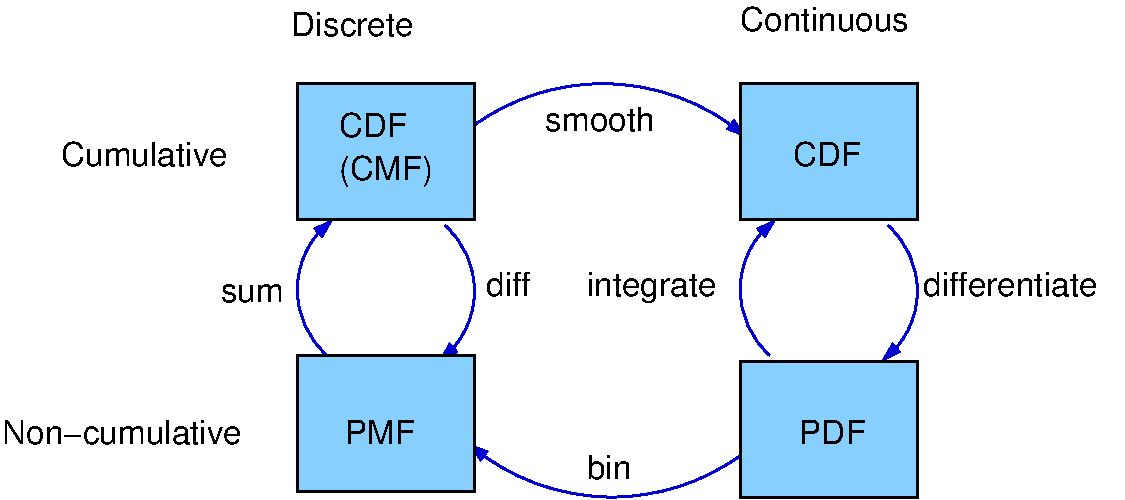
\includegraphics[height=2.2in]{figs/distribution_functions.pdf}}
\caption{A framework that relates representations of distribution
functions.}
\label{dist_framework}
\end{figure}

현재까지 PMF, CDF, PDF를 살펴봤다; 잠시 복습 시간을 가져본다.
그림~\ref{dist_framework}에 함수가 어떻게 서로 연관되는지 나타나 있다.
\index{Pmf}
\index{Cdf}
\index{Pdf}

PMF로 시작했는데, PMF는 이산 집합 값에 대한 확률을 나타낸다.
PMF에서 CDF를 얻기 위해서는, 확률 질량을 더해서 누적 확률을 얻는다.
CDF에서 PMF로 돌아가기 위해서는, 누적 확률 차이를 계산한다.
다음 몇 절에 걸쳐 이와 같은 연산을 어떻게 구현했는지 살펴볼 것이다.
\index{누적 확률 (cumulative probability)}

PDF는 연속형 CDF 미분이다; 혹은, 동등하게 CDF는 PDF의 적분이다.
PDF는 값을 확률 밀도로 매핑한다는 것을 기억하라; 확률값을 얻기 위해서,
적분해야 한다.

\index{이산 분포 (discrete distribution)}
\index{연속 분포 (continuous distribution)}
\index{평활 (smoothing)}

이산형에서 연속 분포를 얻기 위해서, 다양한 평활(smoothing) 작업을 수행할 수 있다.
평활의 한 형태는 데이터가 (지수 혹은 정규 분포처럼) 
해석 연속 분포(analytic continuous distribution)에서 왔다고 가정하는 것이다.
또 다른 선택 옵션은 핵밀도추정(kernel density estimation)이다.

\index{지수 분포 (exponential distribution)}
\index{분포 (distribution)!지수 (exponential)}
\index{정규 분포 (normal distribution)}
\index{분포 (distribution)!정규 (normal)}
\index{가우스 분포 (Gaussian distribution)}
\index{분포 (distribution)!가우스 (Gaussian)}

평활의 반대가 {\bf 이산화 (discretizing)}, 혹은 양자화(quantizing)다.
만약 이산 점에서 PDF를 평가한다면, PDF에 근사하는 PMF를 생성할 수 있다.
수치적분(numerical integration)을 사용해서 좀더 잘 근사할 수도 있다.
\index{이산화 (discretize)}
\index{양자화 (quantize)}
\index{구간화 (binning)}

연속CDF와 이산CDF를 구별하기 위해서, 이산CDF는 
``누적 질량 함수 (cumulative mass function)''가 되는 것이 좋을지도 모른다.
하지만, 저자가 알고 있는 바로는, 누구도 그 용어를 사용하지 않는다.
\index{CDF}



\section{Hist implementation}

At this point you should know how to use the basic types provided
by {\tt thinkstats2}: Hist, Pmf, Cdf, and Pdf.  The next few sections
provide details about how they are implemented.  This material
might help you use these classes more effectively, but it is not
strictly necessary.
\index{Hist}

Hist and Pmf inherit from a parent class called \verb"_DictWrapper".
The leading underscore indicates that this class is ``internal;'' that
is, it should not be used by code in other modules.  The name
indicates what it is: a dictionary wrapper.  Its primary attribute is
{\tt d}, the dictionary that maps from values to their frequencies.
\index{DictWrapper}
\index{internal class}
\index{wrapper}

The values can be any hashable type.  The frequencies should be integers,
but can be any numeric type.
\index{hashable}

\verb"_DictWrapper" contains methods appropriate for both
Hist and Pmf, including \verb"__init__", {\tt Values},
{\tt Items} and {\tt Render}.  It also provides modifier
methods {\tt Set}, {\tt Incr}, {\tt Mult}, and {\tt Remove}.  These
methods are all implemented with dictionary operations.  For example:
\index{dictionary}

\begin{verbatim}
# class _DictWrapper

    def Incr(self, x, term=1):
        self.d[x] = self.d.get(x, 0) + term

    def Mult(self, x, factor):
        self.d[x] = self.d.get(x, 0) * factor

    def Remove(self, x):
        del self.d[x]
\end{verbatim}

Hist also provides {\tt Freq}, which looks up the frequency
of a given value.
\index{frequency}

Because Hist operators and methods are based on dictionaries,
these methods are constant time operations;
that is, their run time does not increase as the Hist gets bigger.
\index{Hist}


\section{Pmf implementation}

Pmf and Hist are almost the same thing, except that a Pmf
maps values to floating-point probabilities, rather than integer
frequencies.  If the sum of the probabilities is 1, the Pmf is normalized.
\index{Pmf}

Pmf provides {\tt Normalize}, which computes the sum of the
probabilities and divides through by a factor:

\begin{verbatim}
# class Pmf

    def Normalize(self, fraction=1.0):
        total = self.Total()
        if total == 0.0:
            raise ValueError('Total probability is zero.')

        factor = float(fraction) / total
        for x in self.d:
            self.d[x] *= factor

        return total
\end{verbatim}

{\tt fraction} determines the sum of the probabilities after
normalizing; the default value is 1.  If the total probability is 0,
the Pmf cannot be normalized, so {\tt Normalize} raises {\tt
  ValueError}.

Hist and Pmf have the same constructor.  It can take
as an argument a {\tt dict}, Hist, Pmf or Cdf, a pandas
Series, a list of (value, frequency) pairs, or a sequence of values.
\index{Hist}

If you instantiate a Pmf, the result is normalized.  If you
instantiate a Hist, it is not.  To construct an unnormalized Pmf,
you can create an empty Pmf and modify it.  The Pmf modifiers do
not renormalize the Pmf.


\section{Cdf implementation}

A CDF maps from values to cumulative probabilities, so I could have
implemented Cdf as a \verb"_DictWrapper".  But the values in a CDF are
ordered and the values in a \verb"_DictWrapper" are not.  Also, it is
often useful to compute the inverse CDF; that is, the map from
cumulative probability to value.  So the implementaion I chose is two
sorted lists.  That way I can use binary search to do a forward or
inverse lookup in logarithmic time.
\index{Cdf}
\index{binary search}
\index{cumulative probability}
\index{DictWrapper}
\index{inverse CDF}
\index{CDF, inverse}

The Cdf constructor can take as a parameter a sequence of values
or a pandas Series, a dictionary that maps from values to
probabilities, a sequence of (value, probability) pairs, a Hist, Pmf,
or Cdf.  Or if it is given two parameters, it treats them as a sorted
sequence of values and the sequence of corresponding cumulative
probabilities.

Given a sequence, pandas Series, or dictionary, the constructor makes
a Hist.  Then it uses the Hist to initialize the attributes:

\begin{verbatim}
        self.xs, freqs = zip(*sorted(dw.Items()))
        self.ps = np.cumsum(freqs, dtype=np.float)
        self.ps /= self.ps[-1]
\end{verbatim}

{\tt xs} is the sorted list of values; {\tt freqs} is the list
of corresponding frequencies.  {\tt np.cumsum} computes
the cumulative sum of the frequencies.  Dividing through by the
total frequency yields cumulative probabilities.
For {\tt n} values, the time to construct the
Cdf is proportional to $n \log n$.
\index{frequency}

Here is the implementation of {\tt Prob}, which takes a value
and returns its cumulative probability: 

\begin{verbatim}
# class Cdf
    def Prob(self, x):
        if x < self.xs[0]:
            return 0.0
        index = bisect.bisect(self.xs, x)
        p = self.ps[index - 1]
        return p
\end{verbatim}

The {\tt bisect} module provides an implementation of binary search.
And here is the implementation of {\tt Value}, which takes a
cumulative probability and returns the corresponding value:

\begin{verbatim}
# class Cdf
    def Value(self, p):
        if p < 0 or p > 1:
            raise ValueError('p must be in range [0, 1]')

        index = bisect.bisect_left(self.ps, p)
        return self.xs[index]
\end{verbatim}

Given a Cdf, we can compute the Pmf by computing differences between
consecutive cumulative probabilities.  If you call the Cdf constructor
and pass a Pmf, it computes differences by calling {\tt Cdf.Items}:
\index{Pmf}
\index{Cdf}

\begin{verbatim}
# class Cdf
    def Items(self):
        a = self.ps
        b = np.roll(a, 1)
        b[0] = 0
        return zip(self.xs, a-b)
\end{verbatim}

{\tt np.roll} shifts the elements of {\tt a} to the right, and ``rolls''
the last one back to the beginning.  We replace the first element of
{\tt b} with 0 and then compute the difference {\tt a-b}.  The result
is a NumPy array of probabilities.
\index{NumPy}

Cdf provides {\tt Shift} and {\tt Scale}, which modify the
values in the Cdf, but the probabilities should be treated as
immutable.


\section{적률 (Moments)}
\index{적률 (moment)}

어느 때고 표본을 얻고 하나의 숫자로 줄일 수 있다. 그 숫자가 통계량(statistic)이다.
지금까지 살펴본 통계량은 평균, 분산, 중위수, 그리고 사분위수다.

{\bf 원적률 (raw moment)}은 일종의 통계량이다. 만약 $x_i$ 표본 값이 있다면,
$k$번째 원적률은 다음과 같다.

%
\[ m'_k = \frac{1}{n} \sum_i x_i^k \]
%
혹은, 파이썬 표기법으로 표현하면, 다음과 같다.

\begin{verbatim}
def RawMoment(xs, k):
    return sum(x**k for x in xs) / len(xs)
\end{verbatim}

$k=1$일 때, 결과는 표본 평균 $\xbar$가 된다.
다른 원적률은 그 자체로 의미가 있지 않다. 하지만, 다른 계산에 사용된다.

{\bf 중심적률(central moments)}이 더 유용하다. 
$k$번째 중심적률은 다음과 같다.
%
\[ m_k = \frac{1}{n} \sum_i (x_i - \xbar)^k \]
%

혹은 파이썬으로 표현하면 다음과 같다.

\begin{verbatim}
def CentralMoment(xs, k):
    mean = RawMoment(xs, 1)
    return sum((x - mean)**k for x in xs) / len(xs)
\end{verbatim}

$k=2$일 때, 결과는 두번째 중심 적률로 분산으로 인지하고 있을 것이다.
분산의 정의가 왜 이러한 통계량이 적률로 불리는지 힌트를 준다.
각 위치 $x_i$에 자를 따라 추를 달고 평균 주위에서 자를 돌리면, 
회전추의 관성 적률은 값의 분산이다. 만약 관성 적률에 익숙하지 않다면,
\url{http://en.wikipedia.org/wiki/Moment_of_inertia} 웹사이트를 참조한다.  
\index{관성 적률(moment of inertia)}

적률에 기반한 통계를 보고할 때, 단위(unit)에 관한 생각이 중요하다.
예를 들어, 값 $x_i$가 cm 이라면, 첫 원적률은 또한 cm이다.
하지만, 두번째 적률은 cm$^2$이고, 세번째 적률은 cm$^3$... 등등이 된다.

이러한 단위 때문에, 적률은 그 자체로 해석하기 어렵다.
두번째 적률에 대해서 분산에 제곱근을 취한 표준편차를 쓰는 것이 이러한 이유다. 
그러면 $x_i$와 단위가 같아진다.
\index{표준 편차 (standard deviation)}


\section{왜도 (Skewness)}
\index{왜도 (skewness)}

{\bf 왜도 (Skewness)}는 분포 형태를 기술하는 속성이다. 
만약 분포가 중심 경향성 주변에서 대칭이라면, 기울어지지 않았다.
만약 값들이 오른쪽으로 좀더 뻗어져 있다면, ``오른쪽으로 기울어져 (right
skewed)'' 있고, 만약 값들이 왼쪽으로 치우쳐 있다면, ``왼쪽으로 기울어져 (left
skewed''있다.

\index{중심 경향성 (central tendency)}

``기울어짐 (skewed)''을 사용하는 것다는 것이 ``편의(biased)''를 함축하지는 않는다.
단지 왜도는 분포 형태만을 기술한다; 표본 추출과정에 편의가 있는지에 관해 
어떤 것도 나타내지 않는다.

\index{편의 (bias)}
\index{표본 왜도 (sample skewness)}

흔히 몇몇 통계량이 분포 왜도를 계량화하는데 사용된다.
주어진 값 시퀀스가 $x_i$가 주어졌을 때, 
{\bf 표본 왜도 (sample skewness)} $g_1$은 다음과 같이 계산된다.

\begin{verbatim}
def StandardizedMoment(xs, k):
    var = CentralMoment(xs, 2)
    std = math.sqrt(var)
    return CentralMoment(xs, k) / std**k

def Skewness(xs):
    return StandardizedMoment(xs, 3)
\end{verbatim}

$g_1$은 제3 표준 적률로 정규화되었다는 것으로 단위가 없다.
\index{표준 적률 (standardized moment)}

음수 왜도는 분포가 왼쪽으로 기울어짐; 양수 왜도는 분포가 오른쪽으로 기울어짐을 
나타낸다. $g_1$의 규모는 왜도 강도를 나타내지만, 그 자체로 해석하기는 쉽지 않다.

실무에서, 표본 왜도를 계산하는 것이 대게 좋은 생각이 되지는 못하다.
만약 어떤 특이점(outlier)이 있다면, $g_1$에 대해서 균형이 맞지 않는 효과를 미친다.
\index{특이점 (outlier)}

분포 비대칭을 평가하는 또 다른 방법은 평균과 중위수 사이 관계를 살펴보는 것이다.
극단값(extreme value)이 중위수보다 평균에 미치는 효과가 더 크다. 그래서 왼쪽으로 기울어진
분포에서 평균은 중위수보다도 더 작다. 오른쪽으로 기울어진 분포에서 평균은 더 크다.

\index{대칭 (symmetric)}
\index{피어슨 중위수 왜도 (Pearson median skewness)}



{\bf 피어슨 중위수 왜도 계수 (Pearson's median skewness coefficient)}는
 표본 평균과 중위수 차이에 기반한 왜도 측도다.
%
\[ g_p = 3 (\xbar - m) / S \]
%
$\xbar$는 표본 평균, $m$은 중위수, $S$는 표준편차다.
혹은 파이썬에서 코드로 작성한 함수는 다음과 같다.
\index{표준편차 (standard deviation)}

\begin{verbatim}
def Median(xs):
    cdf = thinkstats2.Cdf(xs)
    return cdf.Value(0.5)

def PearsonMedianSkewness(xs):
    median = Median(xs)
    mean = RawMoment(xs, 1)
    var = CentralMoment(xs, 2)
    std = math.sqrt(var)
    gp = 3 * (mean - median) / std
    return gp
\end{verbatim}

이 통계량은 {\bf 강건(robust)}해서 의미하는 바는 특이점 때문에 쉽게 휘둘리지 않는다는 것이다.

\index{강건성 (robust)}
\index{특이점 (outlier)}

\begin{figure}
%\centerline{\includegraphics[height=2.2in]{figs/density_totalwgt_kde.pdf}}
\caption{Estimated PDF of birthweight data from the NSFG.}
\label{density_totalwgt_kde}
\end{figure}

예제로 NSFG 임신 데이터에 있는 출생 체중 왜도를 살펴보자.
다음에 PDF를 추정하고 플롯으로 그리는 코드가 있다.
\index{thinkplot}

\begin{verbatim}
    live, firsts, others = first.MakeFrames()
    data = live.totalwgt_lb.dropna()
    pdf = thinkstats2.EstimatedPdf(data)
    thinkplot.Pdf(pdf, label='birth weight')
\end{verbatim}

그림~\ref{density_totalwgt_kde}에 결과가 있다.
왼쪽 꼬리가 오른쪽 꼬리보다 더 길어 보인다. 
그래서 분포가 왼쪽으로 기울어진 것으로 추측해 볼 수 있다.
평균은 7.27 lbs 으로 중위수 7.38 lbs 보다 다소 작아서 왼쪽으로 기울어진 것과
일관성이 있다. 그리고 두 왜도 계수가 모두 음수다: 표본 왜도는  -0.59; 피어슨 중위수 왜도는 -0.23.
\index{왜도 (skewness)}
\index{dropna}
\index{NaN}

\begin{figure}
%\centerline{\includegraphics[height=2.2in]{figs/density_wtkg2_kde.pdf}}
\caption{Estimated PDF of adult weight data from the BRFSS.}
\label{density_wtkg2_kde}
\end{figure}

이제 출생 체중 분포에 대해 BRFSS에 있는 성인 체중 분포와 비교해 보자.
다음에 파이썬 코드가 있다.
\index{thinkplot}

\begin{verbatim}
    df = brfss.ReadBrfss(nrows=None)
    data = df.wtkg2.dropna()
    pdf = thinkstats2.EstimatedPdf(data)
    thinkplot.Pdf(pdf, label='adult weight')
\end{verbatim}

그림~\ref{density_wtkg2_kde}에 결과가 있다.
분포가 오른쪽으로 기울어진 것으로 보인다.
말할 것도 없이, 평균이 79.0으로 중위수 77.3 보다 더 크다.
표본 왜도가 1.1이고 피어슨 중위수 왜도는 0.26이다.
\index{dropna}
\index{NaN}

왜도 계수 부호는 분포가 왼쪽 혹은 오른쪽으로 기울어진 것을 나타내지만,
그것을 제외하고 해석하기는 어렵다.
표본 왜도는 덜 강건하다; 즉, 특이점에 더 좌우된다.
결과로서 덜 믿음이 가는데, 기울어진 분포에 적용될 때, 정확하게 가장 관련될 때 그렇다. 

\index{특이점 (outlier)}
\index{강건성 (robust)}

피어슨 중위수 왜도는 계산된 평균과 분산에 기반한다.
그래서 특이점에 휘둘리기 쉽지만 제3 적률에 의존하지 않기 때문에 좀더 강건하다.
\index{피어스 중위수 왜도 (Pearson median skewness)}


\section{연습문제}

A solution to this exercise is in \verb"chap06soln.py".

\begin{exercise}

The distribution of income is famously skewed to the right.  In this
exercise, we'll measure how strong that skew is.
\index{skewness}
\index{income}

The Current Population Survey (CPS) is a joint effort of the Bureau
of Labor Statistics and the Census Bureau to study income and related
variables.  Data collected in 2013 is available from
\url{http://www.census.gov/hhes/www/cpstables/032013/hhinc/toc.htm}.
I downloaded {\tt hinc06.xls}, which is an Excel spreadsheet with
information about household income, and converted it to {\tt hinc06.csv},
a CSV file you will find in the repository for this book.  You
will also find {\tt hinc2.py}, which reads this file and transforms
the data.
\index{Current Population Survey}
\index{Bureau of Labor Statistics}
\index{Census Bureau}

The dataset is in the form of a series of income ranges and the number
of respondents who fell in each range.  The lowest range includes
respondents who reported annual household income ``Under \$5000.''
The highest range includes respondents who made ``\$250,000 or
more.''

To estimate mean and other statistics from these data, we have to
make some assumptions about the lower and upper bounds, and how
the values are distributed in each range.  {\tt hinc2.py} provides
{\tt InterpolateSample}, which shows one way to model
this data.  It takes a DataFrame with a column, {\tt income}, that
contains the upper bound of each range, and {\tt freq}, which contains
the number of respondents in each frame.
\index{DataFrame}
\index{model}

It also takes \verb"log_upper", which is an assumed upper bound
on the highest range, expressed in {\tt log10} dollars.  
The default value, \verb"log_upper=6.0" represents the assumption
that the largest income among the respondents is
$10^6$, or one million dollars.

{\tt InterpolateSample} generates a pseudo-sample; that is, a sample
of household incomes that yields the same number of respondents
in each range as the actual data.  It assumes that incomes in
each range are equally spaced on a log10 scale.

Compute the median, mean, skewness and Pearson's skewness of the
resulting sample.  What fraction of households reports a taxable
income below the mean?  How do the results depend on the assumed
upper bound?
\end{exercise}


\section{용어 사전}

\begin{itemize}

\item 확률밀도함수 (Probability density function, PDF): 
연속 CDF 미분으로 값을 확률 밀도에 매핑하는 함수.
\index{PDF}
\index{확률밀도함수 (probability density function)}

\item 확률밀도 (Probability density): 
  확률을 만들기 위해서 범위 값에 대해 적분할 수 있는 양.
  예를 들어, 만약 값 단위가 cm이라면, 확률밀도는 cm 당 확률 단위가 된다. 
\index{확률 밀도 (probability density)}

\item 핵밀도추정 (Kernel density estimation, KDE): 
  표본에 기반해서 PDF를 추정하는 알고리즘.
\index{핵밀도추정 (kernel density estimation)}
\index{KDE}

\item 이산화 (discretize): 
  연속함수 혹은 이산 함수를 가진 분포를 근사함. 평활(smoothing)의 반대.
\index{이산화 (discretize)}

\item 원적률 (raw moment): 
  거듭 제곱되는 데이터 합계에 기반한 통계량
\index{원적률 (raw moment)}

\item 중심적률 (central moment): 
  평균에서 편차 거듭제곱에 기반한 통계량.
\index{중심적률 (central moment)}

\item 표준적률 (standardized moment): 
  단위가 없는 적률 비율.
\index{표준적률 (standardized moment)}

\item 왜도 (skewness): 
  분포가 얼마나 비대칭인지 나타내는 측도.
\index{왜도 (skewness)}

\item 표본 왜도 (sample skewness): 
  분포 왜도를 정량화하는데 사용되는 적률기반 통계량.
\index{표본 왜도 (sample skewness)}

\item 피어슨 중위수 왜도 계수 (Pearson's median skewness coefficient): 
  중위수, 평균, 표준편차에 기반한 분포 왜도를 정량화하는데 사용되는 통계량.
  \index{피어슨 중위수 왜도 (Pearson median skewness)}

\item 강건성 (robust): 
  특이점에 상대적으로 면역되어 휘둘리지 않는다면 통계량은 강건하다.
\index{강건성 (robust)}

\end{itemize}




\chapter{변수간 관계}

지금까지 한번에 한 변수만 살펴봤다.
이번장에서 변수간 관계를 살펴본다.
변수 하나를 알고 있는 것이 다른 변수에 대한 정보를 준다면, 두 변수는 관계가 있다.
예를 들어, 신장과 체중은 관계가 있다; 키가 더 큰 사람이 체중이 더 나가는 경향이 있다.
물론, 완벽한 관계는 아니다: 키 작고 뚱뚱한 사람과 키 크고 마른 사람이 있다.
하지만, 다른 사람의 체중을 추측하려고 한다면, 신장 정보를 모르는 것보다 키 정보를 알고 있는 것이
좀더 정확하게 추정하는데 도움이 된다.

\index{성인 체중 (adult weight)}
\index{성인 신장 (adult height)}


이번 장에서 사용되는 코드는 {\tt scatter.py}에 있다.
코드를 다운로드하고 작업하는 것에 대한 정보는 ~\ref{code}을 참조한다.

\section{산점도 (Scatter plots)}
\index{산점도 (scatter plot)}
\index{그림 (plot)!산점도 (scatter)}

관계(relationship)을 확인하는 가장 간단한 방법이 {\bf 산점도 (scatter plot)}다.
하지만, 좋은 산점도를 만드는 것이 항상 쉬운 것은 아니다.
예제로, BRFSS 응답자에 대한 신장과 체중 플롯을 그릴 것이다. (~\ref{lognormal} 절 참조)
\index{BRFSS}

데이터 파일을 읽어서 신장과 체중 정보를 추출하는 코드가 다음에 있다.

\begin{verbatim}
    df = brfss.ReadBrfss(nrows=None)
    sample = thinkstats2.SampleRows(df, 5000)
    heights, weights = sample.htm3, sample.wtkg2
\end{verbatim}

{\tt SampleRows} 함수는 데이터에서 일부를 임으로 골라낸다. 
\index{SampleRows}

\begin{verbatim}
def SampleRows(df, nrows, replace=False):
    indices = np.random.choice(df.index, nrows, replace=replace)
    sample = df.loc[indices]
    return sample
\end{verbatim}

{\tt df}는 데이터프레임이고, {\tt nrows}는 선택할 행의 갯수가 되고, 
{\tt replace}는 복원 추출을 해야 하는지 나타내는 부울(boolean) 표식이다; 
다른 말로, 동일한 행이 한번 이상 선택되어 추출되는지 나타낸다. 

\index{데이터프레임 (DataFrame)}
\index{thinkplot}
\index{부울 (boolean)}
\index{복원 (replacement)}

{\tt thinkplot}에는 {\tt Scatter} 메쏘드가 있는데, 산점도를 그린다.
%
\begin{verbatim}
    thinkplot.Scatter(heights, weights)
    thinkplot.Show(xlabel='Height (cm)',
                   ylabel='Weight (kg)',
                   axis=[140, 210, 20, 200])
\end{verbatim}

그림~\ref{scatter1} (왼쪽)에 관계 형태를 보여주는 결과가 있다.
예상했던 것처럼, 더 키가 큰 사람이 더 체중이 나가는 경향이 있다.

\begin{figure}
% scatter.py
\centerline{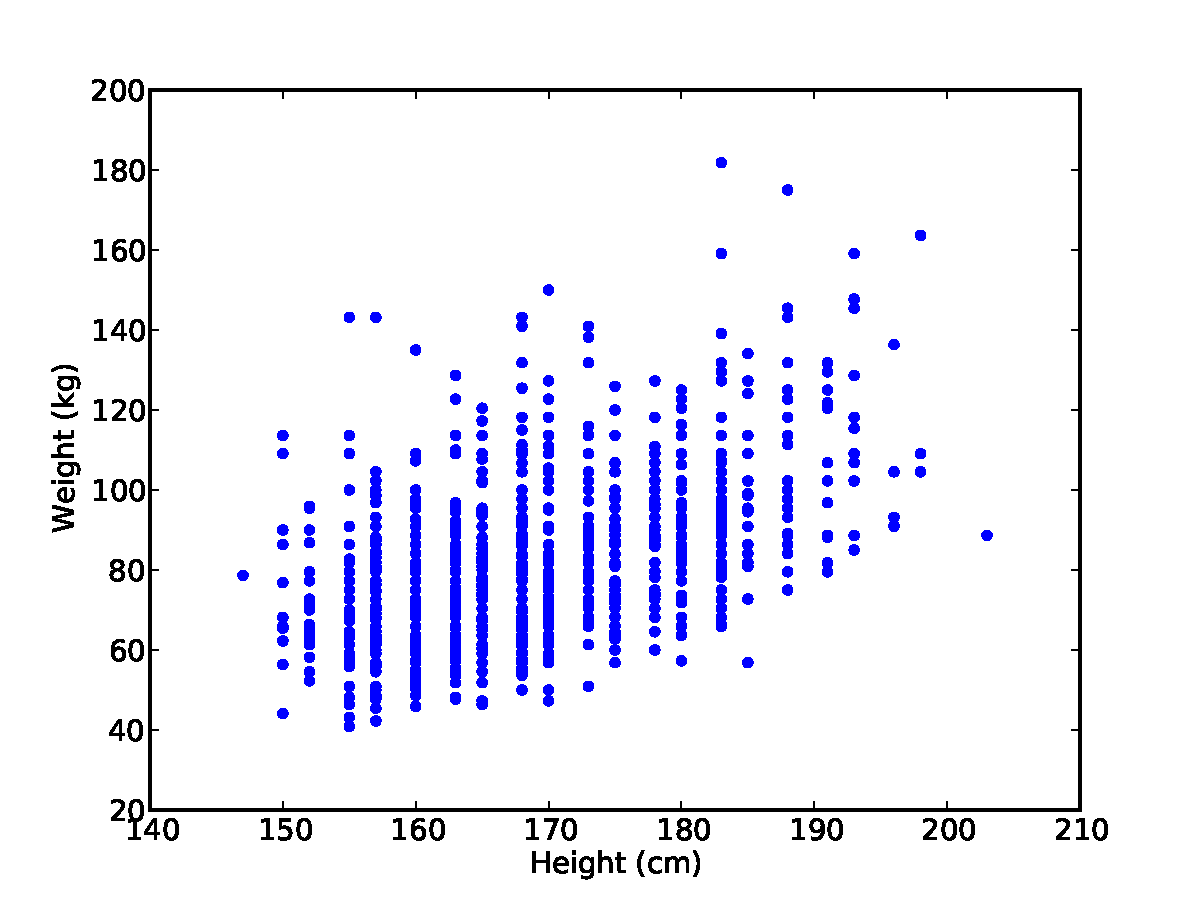
\includegraphics[height=3.0in]{figs/scatter1.pdf}}
\caption{Scatter plots of weight versus height for the respondents
in the BRFSS, unjittered (left), jittered (right).}
\label{scatter1}
\end{figure}

하지만, 상기 그림이 데이터를 가장 잘 표현하는 것은 아니다.
이유는 데이터가 열에 떼지어 몰려있다. 문제는 
신장이 가장 가까운 인치(inch) 단위로 반올림되고, 센티미터로 변환하고 나서,
다시 반올림했다. 변환 과정에서 정보가 유실되었다.

\index{신장 (height)} 
\index{체중 (weight)} 
\index{지터 (jitter)}

유실된 정보를 다시 되돌릴 수는 없지만, 데이터를 {\bf 지터링(jittering)}\footnote{jittering, 지터로 번역을 했는데 통계 사전에는 등록이 되어있지 않고 일반 사전에는 ``조금씩 움직이다''라고 나와있다.}해서 
산점도에 효과를 최소화할 수 있다. 반올림 효과를 되돌리도록 확률 잡음(random noise)를 추가한다는 의미다.
측정값이 가장 근사한 인치(inch) 정보로 반올림되어 있어서, 0.5 인치 즉, 1.3 센티미터까지 차이가 생길 수도 있다. 마찬가지로, 체중은 0.5 kg까지 차이가 생길 수 있다. 

\index{균등 분포 (uniform distribution)}
\index{분포 (distribution)!균등 (uniform)}
\index{잡음 (noise)}

%
\begin{verbatim}
    heights = thinkstats2.Jitter(heights, 1.3)
    weights = thinkstats2.Jitter(weights, 0.5)
\end{verbatim}

{\tt Jitter} 함수를 구현한 것이 다음에 있다.

\begin{verbatim}
def Jitter(values, jitter=0.5):
    n = len(values)
    return np.random.uniform(-jitter, +jitter, n) + values
\end{verbatim}

값은 임의 시퀀스가 될 수 있다; 결과는 넘파이(NumPy) 배열이다.
\index{넘파이 (NumPy)}

그림~\ref{scatter1} (오른편)에 결과가 있다.
지터링(jittering)을 통해서 반올림으로 인한 시각적 효과를 줄이고,
관계 형태를 좀더 명확히 한다. 하지만, 일반적으로 시각화 목적으로만
데이터를 지터링해야 하고, 분석을 위해서 지터링된 데이터 사용은 피해야 한다.

지터링 조차도 데이터를 표현하는 가장 최선의 방법이 되지는 못한다.
중복되는 점이 많아서 그림에서 조밀한 부분에 있는 데이터를 숨기고,
균형이 맞지 않게 특이점을 강조한다. 이와 같은 효과를 {\bf 포화 (saturation)}라고 부른다.
\index{특이점 (outlier)}
\index{포화 (saturation)}

\begin{figure}
% scatter.py
\centerline{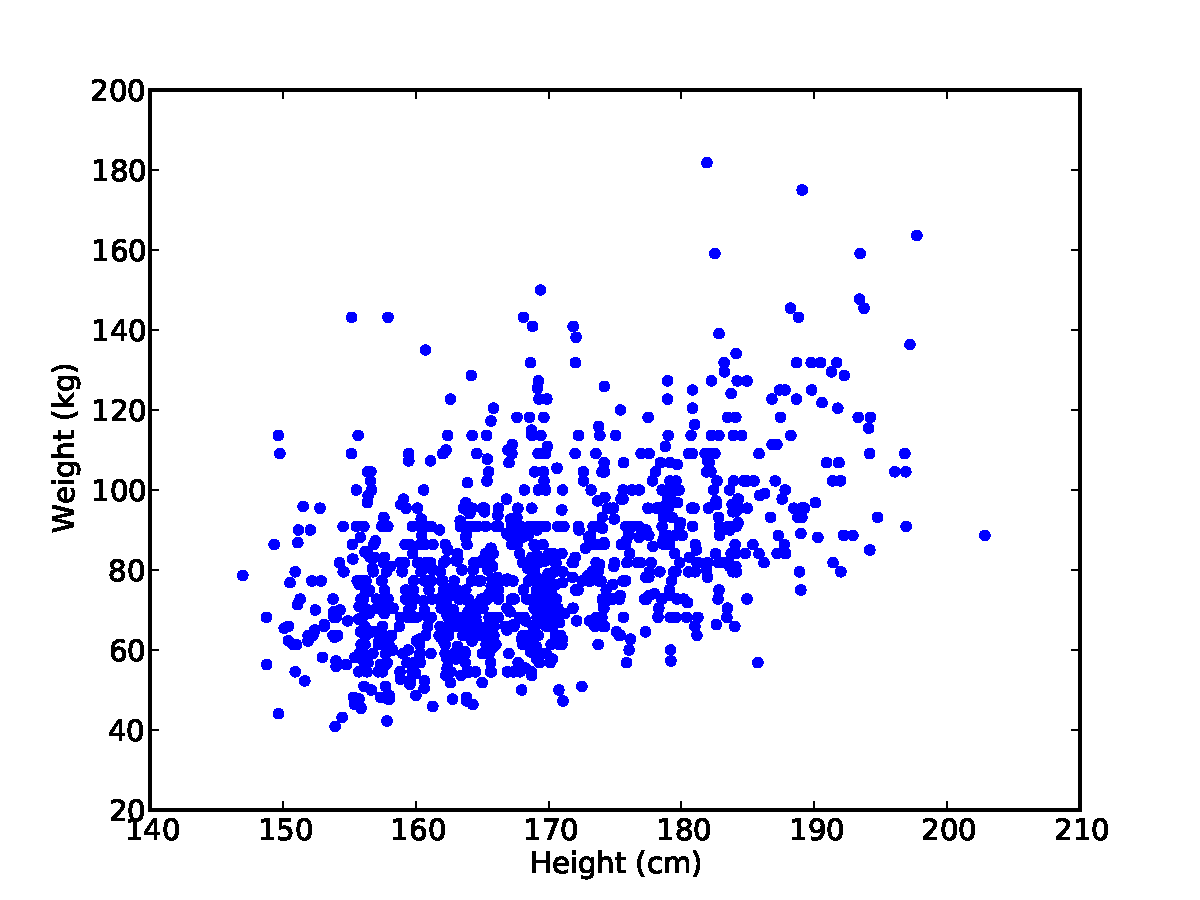
\includegraphics[height=3.0in]{figs/scatter2.pdf}}
\caption{Scatter plot with jittering and transparency (left),
hexbin plot (right).}
\label{scatter2}
\end{figure}

이런 문제를 {\tt alpha} 모수로 해결할 수 있는데, 수행하는 역할은 점들을 부분적으로 투명하게 한다.

%
\begin{verbatim}
    thinkplot.Scatter(heights, weights, alpha=0.2)
\end{verbatim}
%

그림~\ref{scatter2} (왼편)에 결과가 있다.
겹쳐지는 데이터 점들이 더 어두워 보여서 색이 짙음이 밀도와 비례하여 균형을 맞춘다. 이 버젼으로 그린 플롯을 살펴보면, 앞에서 명확하지 않은 두가지 자세한 사항을 볼 수 있다; 90 kg 즉, 200 파운드 근처에 수평선과 몇군데 신장에서 수직 군집이 보인다. 데이터가 파운드 단위로 자기 응답에 기반하기 때문에, 가장 그럴듯한 설명은 응답자가 반올림한 값으로 보고를 한 것이다.

\index{thinkplot}
\index{alpha}
\index{투영성 (transparency)}

투명성을 사용해서 중간정도 크기 데이터셋를 처리했다.
하지만, 그림은 단지 BRFSS 자료 414 509 중에서 첫 5000 레코드만 보여준다.

\index{육각함 플롯 (hexbin plot)}
\index{플롯 (plot)!육각함 (hexbin)}

더 커다란 데이터셋을 처리하기 위한,
또 다른 선택지가 육각함 플롯 (hexbin plot)이 된다.
그래프를 육각형 통(hexagonal bin)으로 나누고 각 통을 얼마나 많은 데이터가 들어있는지에 따라 색을 칠한다. {\tt thinkplot}에 {\tt HexBin}메쏘드가 있다.
%
\begin{verbatim}
    thinkplot.HexBin(heights, weights)
\end{verbatim}
%

그림~\ref{scatter2} (오른편)에 결과가 있다.
육각함(hexbin)의 장점은 관계 형태도 보여준다는 것이고,
큰 데이터셋에 대해서도 시간과 파일 크기에 둘 관점에서 효율적이다.
단점은 특이점이 보이지 않는다는 것이다.
 
\index{thinkplot}
\index{특이점 (outlier)}

이 사례를 통해서 강조하고자 하는 것은 오해를 불러 일으키는 산출물 없이 관계를 명확하게 보여주는 산점도를 플롯으로 그리는 것이 쉬운 것은 아니라는 점이다.

\index{산출물 (artifact)}


\section{Characterizing relationships}
\label{characterizing}

Scatter plots provide a general impression of the relationship between
variables, but there are other visualizations that provide more
insight into the nature of the relationship.  One option is to bin one
variable and plot percentiles of the other.
\index{binning}

NumPy and pandas provide functions for binning data:
\index{NumPy}
\index{pandas}

\begin{verbatim}
    df = df.dropna(subset=['htm3', 'wtkg2'])
    bins = np.arange(135, 210, 5)
    indices = np.digitize(df.htm3, bins)
    groups = df.groupby(indices)
\end{verbatim}

{\tt dropna} drops rows with {\tt nan} in any of the listed columns.
{\tt arange} makes a NumPy array of bins from 135 to, but not including,
210, in increments of 5.
\index{dropna}
\index{digitize}
\index{NaN}

{\tt digitize} computes the index of the bin that contains each value
in {\tt df.htm3}.  The result is a NumPy array of integer indices.
Values that fall below the lowest bin are mapped to index 0.  Values
above the highest bin are mapped to {\tt len(bins)}.

\begin{figure}
% scatter.py
\centerline{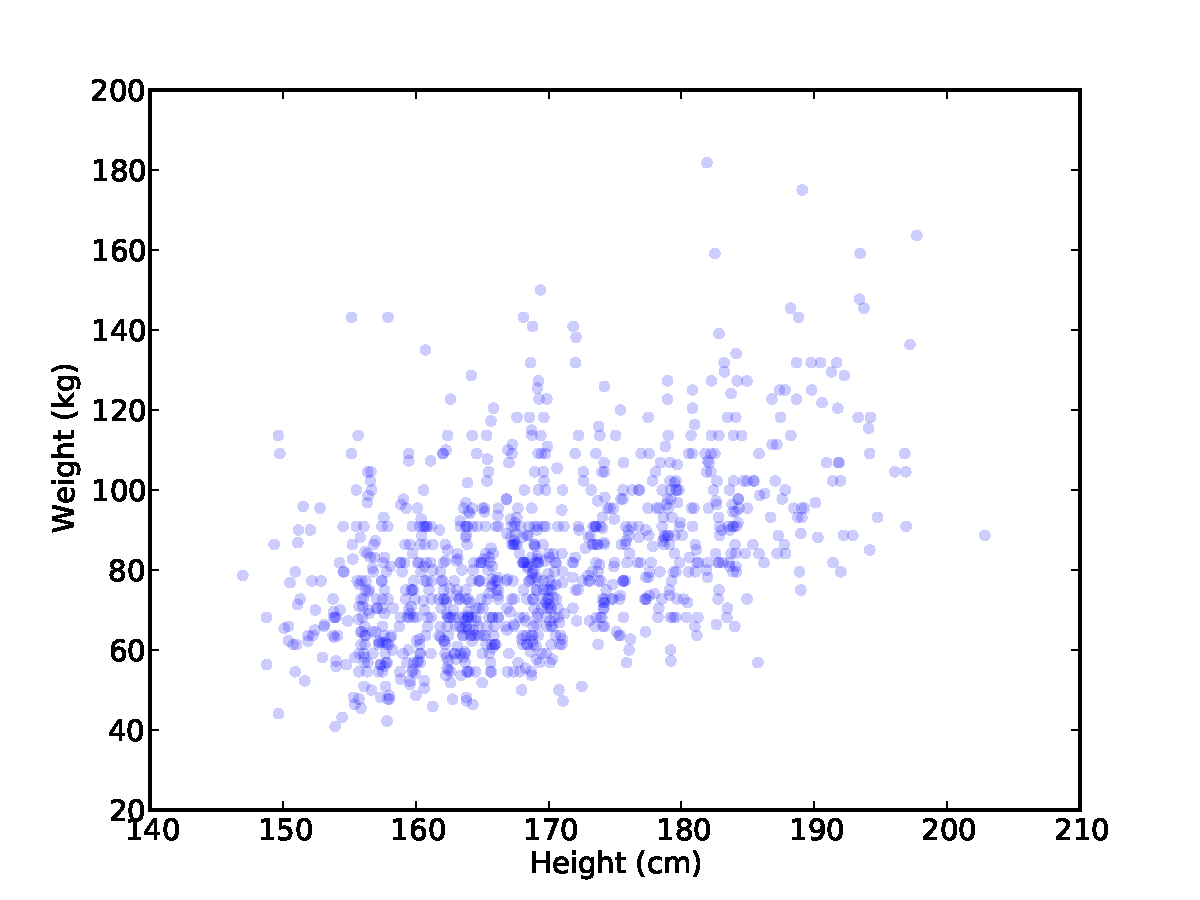
\includegraphics[height=2.5in]{figs/scatter3.pdf}}
\caption{Percentiles of weight for a range of height bins.}
\label{scatter3}
\end{figure}

{\tt groupby} is a DataFrame method that returns a GroupBy object;
used in a {\tt for} loop, {\tt groups} iterates the names of the groups
and the DataFrames that represent them.  So, for example, we can
print the number of rows in each group like this:
\index{DataFrame}
\index{groupby}

\begin{verbatim}
for i, group in groups:
    print(i, len(group))
\end{verbatim}

Now for each group we can compute the mean height and the CDF
of weight:
\index{Cdf}

\begin{verbatim}
    heights = [group.htm3.mean() for i, group in groups]
    cdfs = [thinkstats2.Cdf(group.wtkg2) for i, group in groups]
\end{verbatim}

Finally, we can
plot percentiles of weight versus height:
\index{percentile}

\begin{verbatim}
    for percent in [75, 50, 25]:
        weights = [cdf.Percentile(percent) for cdf in cdfs]
        label = '%dth' % percent
        thinkplot.Plot(heights, weights, label=label)
\end{verbatim}

Figure~\ref{scatter3} shows the result.  Between 140 and 200 cm
the relationship between these variables is roughly linear.  This range
includes more than 99\% of the data, so we don't have to worry
too much about the extremes.
\index{thinkplot}


\section{Correlation}

A {\bf correlation} is a statistic intended to quantify the strength
of the relationship between two variables.
\index{correlation}

A challenge in measuring correlation is that the variables we want to
compare are often not expressed in the same units.  And even if they
are in the same units, they come from different distributions.
\index{units}

There are two common solutions to these problems:

\begin{enumerate}

\item Transform each value to a {\bf standard scores}, which is the
number of standard deviations from the mean.  
This transform leads to
the ``Pearson product-moment correlation coefficient.''
\index{standard score}
\index{standard deviation}
\index{Pearson coefficient of correlation}

\item Transform each value to its {\bf rank}, which is its index in
the sorted list of values.  This transform
leads to the ``Spearman rank correlation coefficient.''
\index{rank}
\index{percentile rank}
\index{Spearman coefficient of correlation}

\end{enumerate}

If $X$ is a series of $n$ values, $x_i$, we can convert to standard
scores by subtracting the mean and dividing by the standard deviation:
$z_i = (x_i - \mu) / \sigma$.
\index{mean}
\index{standard deviation}

The numerator is a deviation: the distance from the mean.  Dividing by
$\sigma$ {\bf standardizes} the deviation, so the values of $Z$ are
dimensionless (no units) and their distribution has mean 0 and
variance 1.
\index{standardize}
\index{deviation}
\index{normal distribution}
\index{distribution!normal}
\index{Gaussian distribution}
\index{distribution!Gaussian}

If $X$ is normally distributed, so is $Z$.  But if $X$ is skewed or has
outliers, so does $Z$; in those cases, it is more robust to use
percentile ranks.  If we compute a new variable, $R$, so that $r_i$ is
the rank of $x_i$, the distribution of $R$ is uniform
from 1 to $n$, regardless of the distribution of $X$.
\index{uniform distribution} \index{distribution!uniform}
\index{robust}
\index{skewness}
\index{outlier}


\section{Covariance}
\index{covariance}
\index{deviation}

{\bf Covariance} is a measure of the tendency of two variables
to vary together.  If we have two series, $X$ and $Y$, their
deviations from the mean are
%
\[ dx_i = x_i - \xbar \]
\[ dy_i = y_i - \ybar \]
%
where $\xbar$ is the sample mean of $X$ and $\ybar$ is the sample mean
of $Y$.  If $X$ and $Y$ vary together, their deviations tend to have
the same sign.

If we multiply them together, the product is positive when the
deviations have the same sign and negative when they have the opposite
sign.  So adding up the products gives a measure of the tendency to
vary together.

Covariance is the mean of these products:
%
\[ Cov(X,Y) = \frac{1}{n} \sum dx_i~dy_i \]
%
where $n$ is the length of the two series (they have to be the same
length).

If you have studied linear algebra, you might recognize that
{\tt Cov} is the dot product of the deviations, divided
by their length.  So the covariance is maximized if the two vectors
are identical, 0 if they are orthogonal, and negative if they
point in opposite directions.  {\tt thinkstats2} uses {\tt np.dot} to
implement {\tt Cov} efficiently:
\index{linear algebra}
\index{dot product}
\index{orthogonal vector}

\begin{verbatim}
def Cov(xs, ys, meanx=None, meany=None):
    xs = np.asarray(xs)
    ys = np.asarray(ys)

    if meanx is None:
        meanx = np.mean(xs)
    if meany is None:
        meany = np.mean(ys)

    cov = np.dot(xs-meanx, ys-meany) / len(xs)
    return cov
\end{verbatim}

By default {\tt Cov} computes deviations from the sample means,
or you can provide known means.  If {\tt xs} and {\tt ys} are
Python sequences, {\tt np.asarray} converts them to NumPy arrays.
If they are already NumPy arrays, {\tt np.asarray} does nothing.
\index{NumPy}

This implementation of covariance is meant to be simple for purposes
of explanation.  NumPy and pandas also provide implementations of
covariance, but both of them apply a correction for small sample sizes
that we have not covered yet, and {\tt np.cov} returns a covariance
matrix, which is more than we need for now.
\index{pandas}


\section{Pearson's correlation}
\index{correlation}
\index{standard score}

Covariance is useful in some computations, but it is seldom reported
as a summary statistic because it is hard to interpret.  Among other
problems, its units are the product of the units of $X$ and $Y$.  For
example, the covariance of weight and height in the BRFSS dataset is
113 kilogram-centimeters, whatever that means.
\index{deviation}
\index{units}

One solution to this problem is to divide the deviations by the standard
deviation, which yields standard scores, and compute the product of
standard scores:
%
\[ p_i = \frac{(x_i - \xbar)}{S_X} \frac{(y_i - \ybar)}{S_Y} \]
%
Where $S_X$ and $S_Y$ are the standard deviations of $X$ and $Y$.
The mean of these products is \index{standard deviation}
%
\[ \rho = \frac{1}{n} \sum p_i \]
%
Or we can rewrite $\rho$ by factoring out $S_X$ and
$S_Y$:
%
\[ \rho = \frac{Cov(X,Y)}{S_X S_Y} \]
%
This value is called {\bf Pearson's correlation} after Karl Pearson,
an influential early statistician.  It is easy to compute and easy to
interpret.  Because standard scores are dimensionless, so is $\rho$.
\index{Pearson, Karl}
\index{Pearson coefficient of correlation}

Here is the implementation in {\tt thinkstats2}:

\begin{verbatim}
def Corr(xs, ys):
    xs = np.asarray(xs)
    ys = np.asarray(ys)

    meanx, varx = MeanVar(xs)
    meany, vary = MeanVar(ys)

    corr = Cov(xs, ys, meanx, meany) / math.sqrt(varx * vary)
    return corr
\end{verbatim}

{\tt MeanVar} computes mean and variance slightly more efficiently
than separate calls to {\tt np.mean} and {\tt np.var}.
\index{MeanVar}

Pearson's correlation is always between -1 and +1 (including both).
If $\rho$ is positive, we say that the correlation is positive,
which means that when one variable is high, the other tends to be
high.  If $\rho$ is negative, the correlation is negative, so
when one variable is high, the other is low.

The magnitude of $\rho$ indicates the strength of the correlation.  If
$\rho$ is 1 or -1, the variables are perfectly correlated, which means
that if you know one, you can make a perfect prediction about the
other.  \index{prediction}

Most correlation in the real world is not perfect, but it is still
useful.  The correlation of height and weight is 0.51, which is a
strong correlation compared to similar human-related variables.


\section{Nonlinear relationships}

If Pearson's correlation is near 0, it is tempting to conclude
that there is no relationship between the variables, but that
conclusion is not valid.  Pearson's correlation only measures {\em
  linear} relationships.  If there's a nonlinear relationship, $\rho$
understates its strength.  \index{linear relationship}
\index{nonlinear}
\index{Pearson coefficient of correlation}

\begin{figure}
\centerline{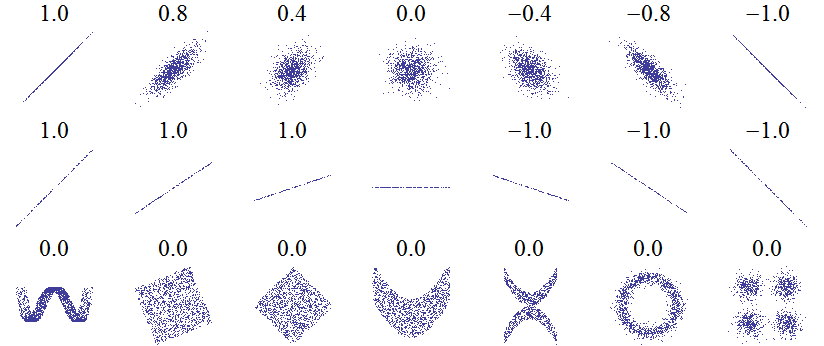
\includegraphics[height=2.5in]{figs/Correlation_examples.png}}
\caption{Examples of datasets with a range of correlations.}
\label{corr_examples}
\end{figure}

Figure~\ref{corr_examples} is from
\url{http://wikipedia.org/wiki/Correlation_and_dependence}.  It shows
scatter plots and correlation coefficients for several
carefully constructed datasets.
\index{scatter plot}
\index{plot!scatter}

The top row shows linear relationships with a range of correlations;
you can use this row to get a sense of what different values of
$\rho$ look like.  The second row shows perfect correlations with a
range of slopes, which demonstrates that correlation is unrelated to
slope (we'll talk about estimating slope soon).  The third row shows
variables that are clearly related, but because the relationship is
nonlinear, the correlation coefficient is 0.
\index{nonlinear}

The moral of this story is that you should always look at a scatter
plot of your data before blindly computing a correlation coefficient.
\index{correlation}


\section{Spearman's rank correlation}

Pearson's correlation works well if the relationship between variables
is linear and if the variables are roughly normal.  But it is not
robust in the presence of outliers.
\index{Pearson coefficient of correlation}
\index{Spearman coefficient of correlation}
\index{normal distribution}
\index{distribution!normal}
\index{Gaussian distribution}
\index{distribution!Gaussian}
\index{robust}
Spearman's rank correlation is an alternative that mitigates the
effect of outliers and skewed distributions.  To compute Spearman's
correlation, we have to compute the {\bf rank} of each value, which is its
index in the sorted sample.  For example, in the sample {\tt [1, 2, 5, 7]}
the rank of the value 5 is 3, because it appears third in the sorted
list.  Then we compute Pearson's correlation for the ranks.
\index{skewness}
\index{outlier}
\index{rank}

{\tt thinkstats2} provides a function that computes Spearman's rank
correlation:

\begin{verbatim}
def SpearmanCorr(xs, ys):
    xranks = pandas.Series(xs).rank()
    yranks = pandas.Series(ys).rank()
    return Corr(xranks, yranks)
\end{verbatim}

I convert the arguments to pandas Series objects so I can use
{\tt rank}, which computes the rank for each value and returns
a Series.  Then I use {\tt Corr} to compute the correlation
of the ranks.
\index{pandas}
\index{Series}

I could also use {\tt Series.corr} directly and specify
Spearman's method:

\begin{verbatim}
def SpearmanCorr(xs, ys):
    xs = pandas.Series(xs)
    ys = pandas.Series(ys)
    return xs.corr(ys, method='spearman')
\end{verbatim}

The Spearman rank correlation for the BRFSS data is 0.54, a little
higher than the Pearson correlation, 0.51.  There are several possible
reasons for the difference, including:
\index{rank correlation}
\index{BRFSS}

\begin{itemize}

\item If the relationship is
nonlinear, Pearson's correlation tends to underestimate the strength
of the relationship, and 
\index{nonlinear}

\item Pearson's correlation can be affected (in either direction)
if one of the distributions is skewed or contains outliers.  Spearman's
rank correlation is more robust.
\index{skewness}
\index{outlier}
\index{robust}

\end{itemize}

In the BRFSS example, we know that the distribution of weights is
roughly lognormal; under a log transform it approximates a normal
distribution, so it has no skew.
So another way to eliminate the effect of skewness is to
compute Pearson's
correlation with log-weight and height:
\index{lognormal distribution}
\index{distribution!lognormal}

\begin{verbatim}
    thinkstats2.Corr(df.htm3, np.log(df.wtkg2)))
\end{verbatim}

The result is 0.53, close to the rank correlation, 0.54.  So that
suggests that skewness in the distribution of weight explains most of
the difference between Pearson's and Spearman's correlation.
\index{skewness}
\index{Spearman coefficient of correlation}
\index{Pearson coefficient of correlation}


\section{Correlation and causation}
\index{correlation}
\index{causation}

If variables A and B are correlated, there are three possible
explanations: A causes B, or B causes A, or some other set of factors
causes both A and B.  These explanations are called ``causal
relationships''.
\index{causal relationship}

Correlation alone does not distinguish between these explanations,
so it does not tell you which ones are true.
This rule is often summarized with the phrase ``Correlation
does not imply causation,'' which is so pithy it has its own
Wikipedia page: \url{http://wikipedia.org/wiki/Correlation_does_not_imply_causation}.

So what can you do to provide evidence of causation?

\begin{enumerate}

\item Use time.  If A comes before B, then A can cause B but not the
  other way around (at least according to our common understanding of
  causation).  The order of events can help us infer the direction
  of causation, but it does not preclude the possibility that something
  else causes both A and B.

\item Use randomness.  If you divide a large sample into two
  groups at random and compute the means of almost any variable, you
  expect the difference to be small.
  If the groups are nearly identical in all variables but one, you
  can eliminate spurious relationships.
  \index{spurious relationship}

  This works even if you don't know what the relevant variables
  are, but it works even better if you do, because you can check that
  the groups are identical.

\end{enumerate}

These ideas are the motivation for the {\bf randomized controlled
trial}, in which subjects are assigned randomly to two (or more)
groups: a {\bf treatment group} that receives some kind of intervention,
like a new medicine, and a {\bf control group} that receives
no intervention, or another treatment whose effects are known.
\index{randomized controlled trial}
\index{controlled trial}
\index{treatment group}
\index{control group}
\index{medicine}

A randomized controlled trial is the most reliable way to demonstrate
a causal relationship, and the foundation of science-based medicine
(see \url{http://wikipedia.org/wiki/Randomized_controlled_trial}).

Unfortunately, controlled trials are only possible in the laboratory
sciences, medicine, and a few other disciplines.  In the social sciences,
controlled experiments are rare, usually because they are impossible
or unethical.
\index{ethics}

An alternative is to look for a {\bf natural experiment}, where
different ``treatments'' are applied to groups that are otherwise
similar.  One danger of natural experiments is that the groups might
differ in ways that are not apparent.  You can read more about this
topic at \url{http://wikipedia.org/wiki/Natural_experiment}.
\index{natural experiment}

In some cases it is possible to infer causal relationships using {\bf
  regression analysis}, which is the topic of Chapter~\ref{regression}.
\index{regression analysis}


\section{Exercises}

A solution to this exercise is in \verb"chap07soln.py".

\begin{exercise}
Using data from the NSFG, make a scatter plot of birth weight
versus mother's age.  Plot percentiles of birth weight
versus mother's age.  Compute Pearson's and Spearman's correlations.
How would you characterize the relationship
between these variables?
\index{birth weight}
\index{weight!birth}
\index{Pearson coefficient of correlation}
\index{Spearman coefficient of correlation}
\end{exercise}


\section{Glossary}

\begin{itemize}

\item scatter plot: A visualization of the relationship between
two variables, showing one point for each row of data.
\index{scatter plot}

\item jitter: Random noise added to data for purposes of
visualization.
\index{jitter}

\item saturation: Loss of information when multiple points are
plotted on top of each other. 
\index{saturation}

\item correlation: A statistic that measures the strength of the
relationship between two variables.
\index{correlation}

\item standardize: To transform a set of values so that their mean is 0 and
their variance is 1.
\index{standardize}

\item standard score: A value that has been standardized so that it is
  expressed in standard deviations from the mean.
  \index{standard score}
\index{standard deviation}

\item covariance: A measure of the tendency of two variables
to vary together.
\index{covariance}

\item rank: The index where an element appears in a sorted list.
\index{rank}

\item randomized controlled trial: An experimental design in which subjects
are divided into groups at random, and different groups are given different
treatments.
\index{randomized controlled trial}

\item treatment group: A group in a controlled trial that receives
some kind of intervention.
\index{treatment group}

\item control group: A group in a controlled trial that receives no
treatment, or a treatment whose effect is known.
\index{control group}

\item natural experiment: An experimental design that takes advantage of
a natural division of subjects into groups in ways that are at least
approximately random.
\index{natural experiment}

\end{itemize}




\chapter{Estimation}
\label{estimation}
\index{estimation}

The code for this chapter is in {\tt estimation.py}.  For information
about downloading and working with this code, see Section~\ref{code}.


\section{The estimation game}

Let's play a game.  I think of a distribution, and you have to guess
what it is.  I'll give you two hints: it's a
normal distribution, and here's a random sample drawn from it:
\index{normal distribution}
\index{distribution!normal}
\index{Gaussian distribution}
\index{distribution!Gaussian}

{\tt [-0.441, 1.774, -0.101, -1.138, 2.975, -2.138]}

What do you think is the mean parameter, $\mu$, of this distribution?
\index{mean}
\index{parameter}

One choice is to use the sample mean, $\xbar$, as an estimate of $\mu$.
In this example, $\xbar$ is 0.155, so it would
be reasonable to guess $\mu$ = 0.155.
This process is called {\bf estimation}, and the statistic we used
(the sample mean) is called an {\bf estimator}.
\index{estimator}

Using the sample mean to estimate $\mu$ is so obvious that it is hard
to imagine a reasonable alternative.  But suppose we change the game by
introducing outliers.
\index{normal distribution}
\index{distribution!normal}
\index{Gaussian distribution}
\index{distribution!Gaussian}

{\em I'm thinking of a distribution.}  It's a normal distribution, and
here's a sample that was collected by an unreliable surveyor who
occasionally puts the decimal point in the wrong place.
\index{measurement error}

{\tt [-0.441, 1.774, -0.101, -1.138, 2.975, -213.8]}

Now what's your estimate of $\mu$?  If you use the sample mean, your
guess is -35.12.  Is that the best choice?  What are the alternatives?
\index{outlier}

One option is to identify and discard outliers, then compute the sample
mean of the rest.  Another option is to use the median as an estimator.
\index{median}

Which estimator is best depends on the circumstances (for example,
whether there are outliers) and on what the goal is.  Are you
trying to minimize errors, or maximize your chance of getting the
right answer?
\index{error}
\index{MSE}
\index{mean squared error}

If there are no outliers, the sample mean minimizes the {\bf mean squared
error} (MSE).  That is, if we play the game many times, and each time
compute the error $\xbar - \mu$, the sample mean minimizes
%
\[ MSE = \frac{1}{m} \sum (\xbar - \mu)^2 \]
%
Where $m$ is the number of times you play the estimation game, not
to be confused with $n$, which is the size of the sample used to
compute $\xbar$.

Here is a function that simulates the estimation game and computes
the root mean squared error (RMSE), which is the square root of
MSE:
\index{mean squared error}
\index{MSE}
\index{RMSE}

\begin{verbatim}
def Estimate1(n=7, m=1000):
    mu = 0
    sigma = 1

    means = []
    medians = []
    for _ in range(m):
        xs = [random.gauss(mu, sigma) for i in range(n)]
        xbar = np.mean(xs)
        median = np.median(xs)
        means.append(xbar)
        medians.append(median)

    print('rmse xbar', RMSE(means, mu))
    print('rmse median', RMSE(medians, mu))
\end{verbatim}

Again, {\tt n} is the size of the sample, and {\tt m} is the
number of times we play the game.  {\tt means} is the list of
estimates based on $\xbar$.  {\tt medians} is the list of medians.
\index{median}

Here's the function that computes RMSE:

\begin{verbatim}
def RMSE(estimates, actual):
    e2 = [(estimate-actual)**2 for estimate in estimates]
    mse = np.mean(e2)
    return math.sqrt(mse)
\end{verbatim}

{\tt estimates} is a list of estimates; {\tt actual} is the
actual value being estimated.  In practice, of course, we don't
know {\tt actual}; if we did, we wouldn't have to estimate it.
The purpose of this experiment is to compare the performance of
the two estimators.
\index{estimator}

When I ran this code, the RMSE of the sample mean was 0.41, which
means that if we use $\xbar$ to estimate the mean of this
distribution, based on a sample with $n=7$, we should expect to be off
by 0.41 on average.  Using the median to estimate the mean yields
RMSE 0.53, which confirms that $\xbar$ yields lower RMSE, at least
for this example.

Minimizing MSE is a nice property, but it's not always the best
strategy.  For example, suppose we are estimating the distribution of
wind speeds at a building site.  If the estimate is too high, we might
overbuild the structure, increasing its cost.  But if it's too
low, the building might collapse.  Because cost as a function of
error is not symmetric, minimizing MSE is not the best strategy.
\index{prediction}
\index{cost function}
\index{MSE}

As another example, suppose I roll three six-sided dice and ask you to
predict the total.  If you get it exactly right, you get a prize;
otherwise you get nothing.  In this case the value that minimizes MSE
is 10.5, but that would be a bad guess, because the total of three
dice is never 10.5.  For this game, you want an estimator that has the
highest chance of being right, which is a {\bf maximum likelihood
  estimator} (MLE).  If you pick 10 or 11, your chance of winning is 1
in 8, and that's the best you can do.  \index{MLE}
\index{maximum likelihood estimator}
\index{dice}


\section{Guess the variance}
\index{variance}
\index{normal distribution}
\index{distribution!normal}
\index{Gaussian distribution}
\index{distribution!Gaussian}

{\em I'm thinking of a distribution.}  It's a normal distribution, and 
here's a (familiar) sample:

{\tt [-0.441, 1.774, -0.101, -1.138, 2.975, -2.138]}

What do you think is the variance, $\sigma^2$, of my distribution?
Again, the obvious choice is to use the sample variance, $S^2$, as an
estimator.
%
\[ S^2 = \frac{1}{n} \sum (x_i - \xbar)^2 \] 
%
For large samples, $S^2$ is an adequate estimator, but for small
samples it tends to be too low.  Because of this unfortunate
property, it is called a {\bf biased} estimator.
An estimator is {\bf unbiased} if the expected total (or mean) error,
after many iterations of the estimation game, is 0.
\index{sample variance}
\index{biased estimator}
\index{estimator!biased}
\index{unbiased estimator}
\index{estimator!unbiased}

Fortunately, there is another simple statistic that is an unbiased
estimator of $\sigma^2$:
%
\[ S_{n-1}^2 = \frac{1}{n-1} \sum (x_i - \xbar)^2 \] 
%
For an explanation of why $S^2$ is biased, and a proof that
$S_{n-1}^2$ is unbiased, see
\url{http://wikipedia.org/wiki/Bias_of_an_estimator}.

The biggest problem with this estimator is that its name and symbol
are used inconsistently.  The name ``sample variance'' can refer to
either $S^2$ or $S_{n-1}^2$, and the symbol $S^2$ is used
for either or both.

Here is a function that simulates the estimation game and tests
the performance of $S^2$ and $S_{n-1}^2$:

\begin{verbatim}
def Estimate2(n=7, m=1000):
    mu = 0
    sigma = 1

    estimates1 = []
    estimates2 = []
    for _ in range(m):
        xs = [random.gauss(mu, sigma) for i in range(n)]
        biased = np.var(xs)
        unbiased = np.var(xs, ddof=1)
        estimates1.append(biased)
        estimates2.append(unbiased)

    print('mean error biased', MeanError(estimates1, sigma**2))
    print('mean error unbiased', MeanError(estimates2, sigma**2))
\end{verbatim}

Again, {\tt n} is the sample size and {\tt m} is the number of times
we play the game.  {\tt np.var} computes $S^2$ by default and
$S_{n-1}^2$ if you provide the argument {\tt ddof=1}, which stands for
``delta degrees of freedom.''  I won't explain that term, but you can read
about it at
\url{http://en.wikipedia.org/wiki/Degrees_of_freedom_(statistics)}.
\index{degrees of freedom}

{\tt MeanError} computes the mean difference between the estimates
and the actual value:

\begin{verbatim}
def MeanError(estimates, actual):
    errors = [estimate-actual for estimate in estimates]
    return np.mean(errors)
\end{verbatim}

When I ran this code, the mean error for $S^2$ was -0.13.  As
expected, this biased estimator tends to be too low.  For $S_{n-1}^2$,
the mean error was 0.014, about 10 times smaller.  As {\tt m}
increases, we expect the mean error for $S_{n-1}^2$ to approach 0.
\index{mean error}

Properties like MSE and bias are long-term expectations based on
many iterations of the estimation game.  By running simulations like
the ones in this chapter, we can compare estimators and check whether
they have desired properties.
\index{biased estimator}
\index{estimator!biased}

But when you apply an estimator to real
data, you just get one estimate.  It would not be meaningful to say
that the estimate is unbiased; being unbiased is a property of the
estimator, not the estimate.

After you choose an estimator with appropriate properties, and use it to
generate an estimate, the next step is to characterize the
uncertainty of the estimate, which is the topic of the next
section.


\section{Sampling distributions}
\label{gorilla}

Suppose you are a scientist studying gorillas in a wildlife
preserve.  You want to know the average weight of the adult
female gorillas in the preserve.  To weigh them, you have
to tranquilize them, which is dangerous, expensive, and possibly
harmful to the gorillas.  But if it is important to obtain this
information, it might be acceptable to weigh a sample of 9
gorillas.  Let's assume that the population of the preserve is
well known, so we can choose a representative sample of adult
females.  We could use the sample mean, $\xbar$, to estimate the
unknown population mean, $\mu$.
\index{gorilla}
\index{population}
\index{sample}

Having weighed 9 female gorillas, you might find $\xbar=90$ kg and
sample standard deviation, $S=7.5$ kg.  The sample mean
is an unbiased estimator of $\mu$, and in the long run it
minimizes MSE.  So if you report a single
estimate that summarizes the results, you would report 90 kg.
\index{MSE}
\index{sample mean}
\index{biased estimator}
\index{estimator!biased}
\index{standard deviation}

But how confident should you be in this estimate?  If you only weigh
$n=9$ gorillas out of a much larger population, you might be unlucky
and choose the 9 heaviest gorillas (or the 9 lightest ones) just by
chance.  Variation in the estimate caused by random selection is
called {\bf sampling error}.
\index{sampling error}

To quantify sampling error, we can simulate the
sampling process with hypothetical values of $\mu$ and $\sigma$, and
see how much $\xbar$ varies.

Since we don't know the actual values of 
$\mu$ and $\sigma$ in the population, we'll use the estimates
$\xbar$ and $S$.
So the question we answer is:
``If the actual values of $\mu$ and $\sigma$ were 90 kg and 7.5 kg,
and we ran the same experiment many times, how much would the
estimated mean, $\xbar$, vary?''

The following function answers that question:

\begin{verbatim}
def SimulateSample(mu=90, sigma=7.5, n=9, m=1000):
    means = []
    for j in range(m):
        xs = np.random.normal(mu, sigma, n)
        xbar = np.mean(xs)
        means.append(xbar)

    cdf = thinkstats2.Cdf(means)
    ci = cdf.Percentile(5), cdf.Percentile(95)
    stderr = RMSE(means, mu)
\end{verbatim}

{\tt mu} and {\tt sigma} are the {\em hypothetical} values of
the parameters.  {\tt n} is the sample size, the number of
gorillas we measured.  {\tt m} is the number of times we run
the simulation.
\index{gorilla}
\index{sample size}
\index{simulation}

\begin{figure}
% estimation.py
%\centerline{\includegraphics[height=2.5in]{figs/estimation1.pdf}}
\caption{Sampling distribution of $\xbar$, with confidence interval.}
\label{estimation1}
\end{figure}

In each iteration, we choose {\tt n} values from a normal
distribution with the given parameters, and compute the sample mean,
{\tt xbar}.  We run 1000 simulations and then compute the
distribution, {\tt cdf}, of the estimates.  The result is shown in
Figure~\ref{estimation1}.  This distribution is called the {\bf
  sampling distribution} of the estimator.  It shows how much the
estimates would vary if we ran the experiment over and over.
\index{sampling distribution}

The mean of the sampling distribution is pretty close
to the hypothetical value of $\mu$, which means that the experiment
yields the right answer, on average.  After 1000 tries, the lowest
result is 82 kg, and the highest is 98 kg.  This range suggests that
the estimate might be off by as much as 8 kg.

There are two common ways to summarize the sampling distribution:

\begin{itemize}

\item {\bf Standard error} (SE) is a measure of how far we expect the
  estimate to be off, on average.  For each simulated experiment, we
  compute the error, $\xbar - \mu$, and then compute the root mean
  squared error (RMSE).  In this example, it is roughly 2.5 kg.
\index{standard error}

\item A {\bf confidence interval} (CI) is a range that includes a
  given fraction of the sampling distribution.  For example, the 90\%
  confidence interval is the range from the 5th to the 95th
  percentile.  In this example, the 90\% CI is $(86, 94)$ kg.
\index{confidence interval}
\index{sampling distribution}

\end{itemize}

Standard errors and confidence intervals are the source of much confusion:

\begin{itemize}

\item People often confuse standard error and standard deviation.
  Remember that standard deviation describes variability in a measured
  quantity; in this example, the standard deviation of gorilla weight
  is 7.5 kg.  Standard error describes variability in an estimate.  In
  this example, the standard error of the mean, based on a sample of 9
  measurements, is 2.5 kg.
\index{gorilla}
\index{standard deviation}

  One way to remember the difference is that, as sample size
  increases, standard error gets smaller; standard deviation does not.

\item People often think that there is a 90\% probability that the
  actual parameter, $\mu$, falls in the 90\% confidence interval.
  Sadly, that is not true.  If you want to make a claim like that, you
  have to use Bayesian methods (see my book, {\it Think Bayes}).
\index{Bayesian statistics}

  The sampling distribution answers a different question: it gives you
  a sense of how reliable an estimate is by telling you how much it
  would vary if you ran the experiment again.
\index{sampling distribution}

\end{itemize}

It is important to remember that confidence intervals
and standard errors only quantify sampling error; that is,
error due to measuring only part of the population.
The sampling distribution does not account for other
sources of error, notably sampling bias and measurement error, 
which are the topics of the next section.


\section{Sampling bias}

Suppose that instead of the weight of gorillas in a nature preserve,
you want to know the average weight of women in the city where you
live.  It is unlikely that you would be allowed
to choose a representative sample of women and
weigh them.
\index{gorilla}
\index{adult weight}
\index{sampling bias}
\index{bias!sampling}
\index{measurement error}

A simple alternative would be
``telephone sampling;'' that is,
you could choose random numbers from the phone book, call and ask to
speak to an adult woman, and ask how much she weighs.
\index{telephone sampling}
\index{random number}

Telephone sampling has obvious limitations.  For example, the sample
is limited to people whose telephone numbers are listed, so it
eliminates people without phones (who might be poorer than average)
and people with unlisted numbers (who might be richer).  Also, if you
call home telephones during the day, you are less likely to sample
people with jobs.  And if you only sample the person who answers the
phone, you are less likely to sample people who share a phone line.

If factors like income, employment, and household size are related
to weight---and it is plausible that they are---the results of your
survey would be affected one way or another.  This problem is
called {\bf sampling bias} because it is a property of the sampling
process.
\index{sampling bias}

This sampling process is also vulnerable to self-selection, which is a
kind of sampling bias.  Some people will refuse to answer the
question, and if the tendency to refuse is related to weight, that
would affect the results.
\index{self-selection}

Finally, if you ask people how much they weigh, rather than weighing
them, the results might not be accurate.  Even helpful respondents
might round up or down if they are uncomfortable with their actual
weight.  And not all respondents are helpful.  These inaccuracies are
examples of {\bf measurement error}.
\index{measurement error}

When you report an estimated quantity, it is useful to report
standard error, or a confidence interval, or both, in order to
quantify sampling error.  But it is also important to remember that
sampling error is only one source of error, and often it is not the
biggest.
\index{standard error}
\index{confidence interval}


\section{Exponential distributions}
\index{exponential distribution}
\index{distribution!exponential}

Let's play one more round of the estimation game.
{\em I'm thinking of a distribution.}  It's an exponential distribution, and 
here's a sample:

{\tt [5.384, 4.493, 19.198, 2.790, 6.122, 12.844]}

What do you think is the parameter, $\lambda$, of this distribution?
\index{parameter}
\index{mean}

\newcommand{\lamhat}{L}
\newcommand{\lamhatmed}{L_m}

In general, the mean of an exponential distribution is $1/\lambda$,
so working backwards, we might choose
%
\[ \lamhat = 1 / \xbar\]
%
$\lamhat$ is an
estimator of $\lambda$.  And not just any estimator; it is also the
maximum likelihood estimator (see
\url{http://wikipedia.org/wiki/Exponential_distribution#Maximum_likelihood}).
So if you want to maximize your chance of guessing $\lambda$ exactly,
$\lamhat$ is the way to go.
\index{MLE}
\index{maximum likelihood estimator}

But we know that $\xbar$ is not robust in the presence of outliers, so
we expect $\lamhat$ to have the same problem.
\index{robust}
\index{outlier}
\index{sample median}

We can choose an alternative based on the sample median.
The median of an exponential distribution is $\ln(2) / \lambda$,
so working backwards again, we can define an estimator
%
\[ \lamhatmed = \ln(2) / m \]
%
where $m$ is the sample median.
\index{median}

To test the performance of these estimators, we can simulate the
sampling process:

\begin{verbatim}
def Estimate3(n=7, m=1000):
    lam = 2

    means = []
    medians = []
    for _ in range(m):
        xs = np.random.exponential(1.0/lam, n)
        L = 1 / np.mean(xs)
        Lm = math.log(2) / thinkstats2.Median(xs)
        means.append(L)
        medians.append(Lm)

    print('rmse L', RMSE(means, lam))
    print('rmse Lm', RMSE(medians, lam))
    print('mean error L', MeanError(means, lam))
    print('mean error Lm', MeanError(medians, lam))
\end{verbatim}

When I run this experiment with $\lambda=2$, the RMSE of $L$ is
1.1.  For the median-based estimator $L_m$, RMSE is 1.8.  We can't
tell from this experiment whether $L$ minimizes MSE, but at least
it seems better than $L_m$.
\index{MSE}
\index{RMSE}

Sadly, it seems that both estimators are biased.  For $L$ the mean
error is 0.33; for $L_m$ it is 0.45.  And neither converges to 0
as {\tt m} increases.
\index{biased estimator}
\index{estimator!biased}

It turns out that $\xbar$ is an unbiased estimator of the mean
of the distribution, $1 / \lambda$, but $L$ is not an unbiased
estimator of $\lambda$.


\section{Exercises}

For the following exercises, you might want to start with a copy of
{\tt estimation.py}.  Solutions are in \verb"chap08soln.py"

\begin{exercise}

In this chapter we used $\xbar$ and median to estimate $\mu$, and
found that $\xbar$  yields lower MSE.
Also, we used $S^2$ and $S_{n-1}^2$ to estimate $\sigma$, and found that
$S^2$ is biased and $S_{n-1}^2$ unbiased.

Run similar experiments to see if $\xbar$ and median are biased estimates
of $\mu$.
Also check whether $S^2$ or $S_{n-1}^2$ yields a lower MSE.
\index{sample mean}
\index{sample median}
\index{estimator!biased}

\end{exercise}


\begin{exercise}

Suppose you draw a sample with size $n=10$ from 
an exponential distribution with $\lambda=2$.  Simulate
this experiment 1000 times and plot the sampling distribution of
the estimate $\lamhat$.  Compute the standard error of the estimate
and the 90\% confidence interval.
\index{standard error}
\index{confidence interval}
\index{sampling distribution}

Repeat the experiment with a few different values of $n$ and make
a plot of standard error versus $n$.
\index{exponential distribution}
\index{distribution!exponential}


\end{exercise}


\begin{exercise}

In games like hockey and soccer, the time between goals is
roughly exponential.  So you could estimate a team's goal-scoring rate
by observing the number of goals they score in a game.  This
estimation process is a little different from sampling the time
between goals, so let's see how it works.
\index{hockey}
\index{soccer}

Write a function that takes a goal-scoring rate, {\tt lam}, in goals
per game, and simulates a game by generating the time between goals
until the total time exceeds 1 game, then returns the number of goals
scored.

Write another function that simulates many games, stores the
estimates of {\tt lam}, then computes their mean error and RMSE.

Is this way of making an estimate biased?  Plot the sampling
distribution of the estimates and the 90\% confidence interval.  What
is the standard error?  What happens to sampling error for increasing
values of {\tt lam}?
\index{estimator!biased}
\index{biased estimator}
\index{standard error}
\index{confidence interval}

\end{exercise}


\section{Glossary}

\begin{itemize}

\item estimation: The process of inferring the parameters of a distribution
from a sample.
\index{estimation}

\item estimator: A statistic used to estimate a parameter.
\index{estimation}

\item mean squared error (MSE): A measure of estimation error.
\index{mean squared error}
\index{MSE}

\item root mean squared error (RMSE): The square root of MSE,
a more meaningful representation of typical error magnitude.
\index{mean squared error}
\index{MSE}

\item maximum likelihood estimator (MLE): An estimator that computes the
point estimate most likely to be correct.
\index{MLE}
\index{maximum likelihood estimator}

\item bias (of an estimator): The tendency of an estimator to be above or
  below the actual value of the parameter, when averaged over repeated
  experiments.  \index{biased estimator}

\item sampling error: Error in an estimate due to the limited
  size of the sample and variation due to chance. \index{point estimation}

\item sampling bias: Error in an estimate due to a sampling process
  that is not representative of the population. \index{sampling bias}

\item measurement error: Error in an estimate due to inaccuracy collecting
  or recording data. \index{measurement error}

\item sampling distribution: The distribution of a statistic if an
  experiment is repeated many times.  \index{sampling distribution}

\item standard error: The RMSE of an estimate,
which quantifies variability due to sampling error (but not
other sources of error).
\index{standard error}

\item confidence interval: An interval that represents the expected
  range of an estimator if an experiment is repeated many times.
  \index{confidence interval} \index{interval!confidence}

\end{itemize}



\chapter{가설 검정 (Hypothesis testing)}
\label{testing}

이번 장에서 사용되는 코드는 {\tt hypothesis.py}에 있다.
코드를 다운로드하고 작업하는 것에 대한 정보는 ~\ref{code}을 참조한다.


\section{전통적 가설 검정 (Classical hypothesis testing)}
\index{가설 검정 (hypothesis testing)}
\index{외관 효과 (apparent effect)}

NSFG에서 데이터를 탐색하면서, 첫째 아이와 첫째가 아닌 아이들 간 차이를 
포함해서 몇가지 ``외관 효과 (apparent effects)''를 봤다.
지금까지 액면 그대로 이러한 효과를 받아들였다; 이번 장에서 이를 검정한다. 

\index{국가 가정 성장 조사 (National Survey of Family Growth)}
\index{NSFG}

다루고자 하는 근본적인 질문은 표본에서 본 효과가 더 큰 모집단에서 나타날 것인가다.
예를 들어, NSFG 표본에서 첫째 아이와 첫째 아이가 아닌 아이들에 대한 평균 임신 기간에
차이를 봤다. 알고자 하는 것은 이 효과가 미국 여성에 대한 진정한 차이를 반영하는지 
혹은, 우연히 표본에서 생겨난 것이냐다.
\index{임신 기간 (pregnancy length)} 
\index{기간 (length)!임신 (pregnancy)}

피셔 귀무 가설 검정(Fisher null hypothesis testing), 네이만 피어슨 의사결정 이론(Neyman-Pearson decision theory), 베이즈 추론(Bayesian inference)\footnote{베이즈 추론에 대한 좀더 많은 정보는 후속해서 출간되는 {\it Think Bayes}를 참조한다.}을 포함해서 질문을 구성하는 방법이 몇가지 있다.
여기 제시하는 것은 대부분의 사람이 실무에서 사용하는 세가지 방법의 일부분으로 {\bf 전통적 가설 검정 (classical hypothesis testing)}이라고 저자가 작명한 것이다.
\index{베이즈 추론 (Bayesian inference)}
\index{귀무 가설 (null hypothesis)}

전통적 가설 검정의 목적은 다음 질문에 답하는 것이다.
``표본과 명백한 효과가 주어졌다면, 우연히 그런 효과를 목도하는 확률이 얼마인가?''
다음에 질문에 답을 하는 방법이 있다.

\begin{itemize}

\item 첫번째 단계는 {\bf 검정 통계량 (test statistic)}을 선택해서 
외관 효과 크기를 정량화한다. NSFG 예제에서, 명백한 효과는 첫번째 아이와 첫째가 아닌 아이들 사이에 임신 기간에 차이가 된다. 그래서, 검정 통계량에 대한 자연스러운 선택이
두 집단 사이에 평균 차이가 된다.
  \index{검정 통계량 (test statistic)}

\item 두번째 단계는 {\bf 귀무 가설 (null hypothesis)}을 정의하는 것으로,
명백한 효과가 사실이 아니라는 가정에 기반한 시스템 모형이다.
NSFG 예제에서, 귀무 가설은 첫째 아이와 첫째가 아닌 아이들 사이에 차이가 없다가 된다;
즉, 두 집단 임신 기간은 동일한 분포다. 
\index{귀무 가설 (null hypothesis)}
\index{임신 기간 (pregnancy length)}
\index{모형 (model)}

\item 세번째 단계는 {\bf p-값(p-value)}을 계산하는 것으로, 만약 귀무 가설이 사실이라면 명백한 효과를 볼 확률값이 된다. NSFG 예제에서, 평균에 실제 차이를 계산하고 나서, 귀무 가설 아래에서 차이를 크게 혹은 더 크게 볼 확률을 계산한다.
\index{p-값 (p-value)}

\item 마지막 단계는 결과를 해석하는 것이다. 만약 p-값이 낮다면, 효과에 
{\bf 통계적 유의성 (statistically significant)}이 있다고 한다.
우연히 발생할 것 같지 않다는 의미가 된다. 이 경우 더 큰 모집단에서 효과가 나타날 것 같다고 추론한다.\index{통계적 유의성 (statistically significant)} 
\index{유의성 (significant)}

\end{itemize}

이 과정의 로직(logic)은 모순(contradiction)에 의한 증명과 유사하다. 
수학 명제(mathematical statement) A를 증명하기 위해, 일시적으로 A 가 거짓이라고 가정한다.
만약 가정이 모순을 이끌게 되면, A 는 사실 참이어야 한다고 결론낸다.

\index{모순, 증명 (contradiction, proof by)}
\index{모순에 의한 증명 (proof by contradiction)}

유사하게, ``효과가 사실 (This effect is real)'' 같은 가설을 검정하기 위해서,
일시적으로 효과가 없다고 가정한다. 이것이 귀무가설이다.
이 가정에 기반해서, 외관 효과 확률을 계산한다. 이것이 p-값이다.
만약 p-값이 작다면, 귀무 가설이 사실이 아닐 것 같다고 결론낸다.

\index{p-값 (p-value)}
\index{귀무 가설 (null hypothesis)}


\section{HypothesisTest}
\label{hypotest}
\index{평균 (mean)!차이 (difference in)}

{\tt thinkstats2}에는 전통적 가설 검정 구조를 표현하는 {\tt HypothesisTest} 클래스가 있다.

다음에 클래스 정의가 있다.
\index{HypothesisTest}

\begin{verbatim}
class HypothesisTest(object):

    def __init__(self, data):
        self.data = data
        self.MakeModel()
        self.actual = self.TestStatistic(data)

    def PValue(self, iters=1000):
        self.test_stats = [self.TestStatistic(self.RunModel()) 
                           for _ in range(iters)]

        count = sum(1 for x in self.test_stats if x >= self.actual)
        return count / iters

    def TestStatistic(self, data):
        raise UnimplementedMethodException()

    def MakeModel(self):
        pass

    def RunModel(self):
        raise UnimplementedMethodException()
\end{verbatim}

{\tt HypothesisTest}는 추상 부모 클래스로 메쏘드 몇개에 대한 완전한 정의와 
다른 메쏘드를 위한 자리잡기(place-keeper) 기능 제공한다.
{\tt HypothesisTest}에 기반한 자식 클래스는 \verb"__init__"와 {\tt PValue} 을 상속받고, {\tt TestStatistic}, {\tt RunModel}, 그리고 선택옵션으로 {\tt MakeModel} 메쏘드를 제공한다.
\index{HypothesisTest}

\verb"__init__"은 적절한 어떤 형식의 데이터도 받아들인다.
{\tt MakeModel} 호출해서 귀무 가설을 표현을 구축하고 나서,
데이터를 {\tt TestStatistic}에 전달하고 표본 효과 크기를 계산한다.

\index{검정 통계량 (test statistic)}
\index{귀무 가설 (null hypothesis)}

{\tt PValue}는 귀무 가설 아래에서 외관 효과 확률을 계산한다.
매개 변수로 {\tt iters}을 받는데 실행할 모의 시험 횟수다.
첫번째 행은 모의 시험 데이터를 생성하고, 검정 통계량을 계산하고, 
\verb"test_stats"에 저장한다.
결과는 관측된 검정 통계량 {\tt self.actual}와 동일하거나 큰 \verb"test_stats" 에 있는 비율이다.
\index{모의 시험 (simulation)}

간단한 예제\footnote{인용 출처: MacKay, {\it Information
Theory, Inference, and Learning Algorithms}, 2003.}로, 250번 동전을 던져서 앞면 140회, 뒷면 110회 나왔다고 가정하자.
이 결과에 기초하여, 동전에 편의가 있는지 의심할지도 모른다; 즉, 좀더 앞면이 나올 것 같다.
이 가설을 검정하기 위해서, 확률을 계산해서 만약 동전이 정말 공정하다면, 그런 차이가 있는지 살펴본다.

\index{편의 동전 (biased coin)}
\index{MacKay, David}

\begin{verbatim}
class CoinTest(thinkstats2.HypothesisTest):

    def TestStatistic(self, data):
        heads, tails = data
        test_stat = abs(heads - tails)
        return test_stat

    def RunModel(self):
        heads, tails = self.data
        n = heads + tails
        sample = [random.choice('HT') for _ in range(n)]
        hist = thinkstats2.Hist(sample)
        data = hist['H'], hist['T']
        return data
\end{verbatim}

모수 {\tt data}는 정수 짝이다: 앞면 숫자, 뒷면 숫자.
검정 통계량은 둘 사이 절대값 차이다. 그래서 {\tt self.actual}은 30 이다.
\index{HypothesisTest}

{\tt RunModel}은 동전이 정말 공정하다고 가정하고 동전던지기를 모의 시험한다.
250번 동전던지기 표본을 생성하고, Hist를 사용해서 앞면과 뒷면 횟수를 계수하고 나서,
정수 짝을 반환한다.
\index{Hist}
\index{모형 (model)}

이제 해야할 일은 {\tt CoinTest} 인스턴스화 하고, {\tt PValue}를 호출한다.

\begin{verbatim}
    ct = CoinTest((140, 110))
    pvalue = ct.PValue()
\end{verbatim}

결과는 약 0.07 이 된다. 만약 동전이 공정하다면, 30 만큼 차이는 이번에 약 7\% 확률로 기대할 수 있다.

이러한 결과를 어떻게 해석해야 할까요? 통상 관례로, 5\%가 통계적 유의성의 임계치다.
만약 p-값이 5\%보다 적다면, 효과가 유의적이라고 생각하고; 그렇지 않다면, 반대로 생각한다.

\index{p-값 (p-value)}
\index{통계적 유의성 (statistically significant)} 
\index{유의성 (significant)}

하지만, 5\% 선택은 작위적이고, (나중에 살펴보겠지만) p-값은 검정 통계량과 귀무 가설 모형에 의존성이 있다.
그래서, p-값이 정밀한 측정으로 생각하지는 말아야 한다.
\index{귀무 가설 (null hypothesis)}

p-값을 해석함에 있어 저자가 추전하는 것은 p-값 크기에 따라 달리하는 것이다:
만약 p-값이 1\%보다 작다면 효과가 우연에 의한 것일 것 같지는 않다;
만약 p-값이 10\%보다 크다면, 효과는 우연으로 설명될 수 있을 것 같다.
p-값이 1\%과 10\% 사이라면, 경계값으로 생각해야한다. 그래서, 상기 사례를 통해서는 
동전에 편의가 있는지 없는지 데이터가 강력한 증거를 주지는 못한다고 결론낸다. 

\section{평균 차이 검정 (Testing a difference in means)}
\label{testdiff}
\index{평균 (mean)!차이 (difference in)}

검정할 가장 일반적인 효과중의 하나가 두 그룹 사이 평균 차이다.
NSFG 데이터에서 첫번째 아이에 대한 평균 임신기간이 약간 더 길었고,
평균 출산 체중은 약간 더 적었다. 이제 이러한 효과가 통계적으로 유의적인지 살펴보자.

\index{국가 가족 성장 조사 (National Survey of Family Growth)}
\index{NSFG}
\index{임신 기간 (pregnancy length)}
\index{기간 (length)!임신 (pregnancy)}

이 예제에서, 귀무가설은 두 집단에 대한 분포가 동일하다는 것이다.
귀무 가설을 모형화하는 한 방법은 {\bf 순열(permutation)}에 의한 것이다; 즉, 첫번째 아이와 첫째가 아닌 아이들에 대한 값을 뽑아서 뒤섞어서, 두 집단을 하나의 큰 집단으로 처리한다.

\index{귀무 가설 (null hypothesis)}
\index{순열 (permutation)}
\index{모형 (model)}

\begin{verbatim}
class DiffMeansPermute(thinkstats2.HypothesisTest):

    def TestStatistic(self, data):
        group1, group2 = data
        test_stat = abs(group1.mean() - group2.mean())
        return test_stat

    def MakeModel(self):
        group1, group2 = self.data
        self.n, self.m = len(group1), len(group2)
        self.pool = np.hstack((group1, group2))

    def RunModel(self):
        np.random.shuffle(self.pool)
        data = self.pool[:self.n], self.pool[self.n:]
        return data
\end{verbatim}

{\tt data}는 한쌍 시퀀스로 각 시퀀스는 각 집단이 된다.
검정 통계량은 평균에 있어 절대값 차이다.
\index{HypothesisTest}

{\tt MakeModel}은 집단 크기 {\tt n}과 {\tt m}을 기록하고
집단을 넘파이(NumPy) 배열 {\tt self.pool}에 결합한다.
\index{NumPy}

{\tt RunModel}은 합동값(pooled value)을 뒤섞고 두 집단 {\tt n}과 {\tt m}으로 쪼개서 귀무가설을 모의 시험한다.
항상 그렇지만, {\tt RunModel}에서 반환되는 값은 관측 데이터와 동일한 형식이다.
\index{귀무 가설 (null hypothesis)}
\index{모형 (model)}

임신 기간에 차이를 검정하기 위해서, 다음을 실행한다. 

\begin{verbatim}
    live, firsts, others = first.MakeFrames()
    data = firsts.prglngth.values, others.prglngth.values
    ht = DiffMeansPermute(data)
    pvalue = ht.PValue()
\end{verbatim}

{\tt MakeFrames}는 NSFG 데이터를 읽고, 모든 정상출산, 첫째 아이, 첫째가 아닌 아이들을 대표하는 데이터프레임을 반환한다.
임신 기간을 넘파이(NumPy) 배열로 추출하고, 데이터로 {\tt DiffMeansPermute}에 전달하고, p-값을 계산한다.
결과는 약 0.17로 의미하는 바는 약 17\% 정도 관측된 효과에 차이를 예상할 수 있다. 그래서, 효과가 통계적으로 유의하지 않다.

\index{데이터프레임 (DataFrame)}
\index{p-값 (p-value)}
\index{유의성 (significant)} 
\index{통계적 유의성 (statistically significant)}
\index{임신 기간 (pregnancy length)}

\begin{figure}
% hypothesis.py
%\centerline{\includegraphics[height=2.5in]{figs/hypothesis1.pdf}}
\caption{CDF of difference in mean pregnancy length under the null
hypothesis.}
\label{hypothesis1}
\end{figure}

{\tt HypothesisTest}에는 {\tt PlotCdf}가 있는데 관측 효과 크기를 나타내는 회색선과 검정 통계량 분포를 플롯으로 그린다.
\index{thinkplot}
\index{HypothesisTest}
\index{Cdf}
\index{효과 크기 (effect size)}

\begin{verbatim}
    ht.PlotCdf()
    thinkplot.Show(xlabel='test statistic',
                   ylabel='CDF')
\end{verbatim}

그림~\ref{hypothesis1}에 결과가 있다.
CDF는 0.83에서 관측 차이와 교차하는데, p-값의 보수 0.17이다.

 shows the result.  The CDF intersects the
observed difference at 0.83, which is the complement of the p-value,
0.17.
\index{p-값 (p-value)}

만약 출생 체중으로 동일한 분석을 실행한다면, 계산된 p-값은 0 이다; 1000 번 시험 후에, 모의시험은 결코 관측 차이가 0.12 lbs 보다 큰 효과를 산출하지 못한다.
그래서, $p < 0.001$ 가 나오고, 출생 체중에 차이는 통계적으로 유의하다고 결론낸다. 

\index{출생 체중 (birth weight)}
\index{체중 (weight)!출생 (birth)}
\index{유의성 (significant)} 
\index{통계적 유의성 (statistically significant)}


\section{다른 검정 통계량 (ther test statistics)}

최선의 검정 통계량을 고르는 것은 무슨 질문을 하느냐에 달려 있다.
예를 들어, 만약 관련된 질문이 첫번째 아이에 대해서 임신 기간이 다른지에 관한 것이라면, 앞절에서 수행했던 것과 같이, 평균에 대해 차이 절대값을 검정하는 것이 의미가 있다.

\index{검정 통계량 (test statistic)}
\index{임신 기간 (pregnancy length)}

만약 첫번째 아이가 늦게 출생하는 경향이 있다고 생각할 이유가 있다면, 차이값의 절대값을 취하지 않는다; 대신에 다음 검정 통계량을 사용한다.

\begin{verbatim}
class DiffMeansOneSided(DiffMeansPermute):

    def TestStatistic(self, data):
        group1, group2 = data
        test_stat = group1.mean() - group2.mean()
        return test_stat
\end{verbatim}

{\tt DiffMeansOneSided}은 {\tt DiffMeansPermute}에서 {\tt MakeModel}와 {\tt RunModel}을 상속받는다; 유일한 차이는 {\tt TestStatistic}가 
차이에 절대값을 취하지 않는다는 것이다.
이런 유형의 검증을 {\bf 단측 (one-sided)} 검증이라고 한다. 왜냐하면,
차이 분포의 단측면만 고려하기 때문이다. 앞선 검정은 양쪽을 사용하기 때문에 {\bf 양측 (two-sided)} 검증이라고 한다.
\index{단측 검증 (one-sided test)}
\index{양측 검증 (two-sided test)}

이 버젼 검정에 대해서, p-값은 0.09 다. 일반적으로 단측 검정에 대한 p-값은 양측 검정에 대한 p-값의 약 절반이다. 물론 분포 모양에 달려있다.

\index{p-값 (p-value)}

단측 가설, 첫째 아이가 늦게 태어난다는 것이 양측 가설보다 좀더 구체적이다. 그래서 p-값이 더 작다. 하지만, 더 강한 가정에 조차도, 차이는 통계적으로 유의적이지 않다.

\index{유의성 (significant)} 
\index{통계적 유의성 (statistically significant)}

동일한 프레임워크(framework)를 사용해서 표준 편차에 차이도 검정할 수 있다. 
~\ref{visualization} 절에서 첫번째 아이가 늦게 혹은 빨리 출산할 것같은 증거를 일부 보았다. 그래서, 표준 편차가 좀더 클 것이라는 가설을 세울 수 있다. 다음에 이 가설을 시험하는 방법이 있다.

\index{표준 편차 (standard deviation)}

\begin{verbatim}
class DiffStdPermute(DiffMeansPermute):

    def TestStatistic(self, data):
        group1, group2 = data
        test_stat = group1.std() - group2.std()
        return test_stat
\end{verbatim}

이것은 단측 검정인데 이유는 가설이 첫번째 아이 집단에 대한 표준편차가 단지 다르다는 것이 아니라 더 높다는 것이다. p-값이 0.09로, 통계적으로 유의적이지 않다.

\index{p-값 (p-value)}
\index{순열 (permutation)}
\index{유의성 (significant)} 
\index{통계적 유의성 (statistically significant)}


\section{상관 검정 (Testing a correlation)}
\label{corrtest}

상기 프레임워크를 사용해서 상관도 검정할 수 있다. 
예를 들어, NSFG 데이터셋에서, 산모 나이와 출생 체중 사이 상관관계는 약 0.07 이다. 
나이가 많은 산모 아이가 더 체중이 나가는 것처럼 보인다. 하지만 이 효과가 우연에 의한 것일까요?
\index{상관 (correlation)}
\index{검정 통계량 (test statistic)}

검정 통계량으로, 피어슨 상관을 사용했지만, 스피어만 상관도 동일하게 동작한다. 만약 양의 상관 관계로 예측하는 합리적 논거가 있다면, 단측 검정을 할 수도 있다. 하지만, 그런 이유가 없기 때문에, 상관 절대값을 사용해서 양측검정을 수행한다.
\index{피어슨 상관계수 (Pearson coefficient of correlation)}
\index{스피어만 상관계수 (Spearman coefficient of correlation)}

귀무 가설은 산모 연령과 출생 체중 사이에 상관 관계가 없다는 것이다.
관측값을 뒤섞어서, 산모 연령과 출생 체중 분포가 같지만 변수 사이에 관련이 없는 세상을 모의 시험할 수 있다.
\index{출생 체중 (birth weight)}
\index{체중 (weight)!출생 (birth)}
\index{귀무 가설 (null hypothesis)}

\begin{verbatim}
class CorrelationPermute(thinkstats2.HypothesisTest):

    def TestStatistic(self, data):
        xs, ys = data
        test_stat = abs(thinkstats2.Corr(xs, ys))
        return test_stat

    def RunModel(self):
        xs, ys = self.data
        xs = np.random.permutation(xs)
        return xs, ys
\end{verbatim}

{\tt data}는 한쌍 시퀀스다. {\tt TestStatistic}가 피어슨 상관 절대값을 계산한다. {\tt RunModel}이 {\tt xs}를 뒤섞고 모의시험한 데이터를 반환한다.
\index{HypothesisTest}
\index{순열 (permutation)}
\index{피어슨 상관계수 (Pearson coefficient of correlation)}

다음에 데이터를 읽어 들이고, 시험을 수행하는 코드가 있다.

\begin{verbatim}
    live, firsts, others = first.MakeFrames()
    live = live.dropna(subset=['agepreg', 'totalwgt_lb'])
    data = live.agepreg.values, live.totalwgt_lb.values
    ht = CorrelationPermute(data)
    pvalue = ht.PValue()
\end{verbatim}

{\tt subset} 인자로 {\tt dropna}를 사용해서 필요한 변수 둘 중에서 결측된 행을 뺀다.
\index{dropna}
\index{NaN}
\index{결측값 (missing values)}

실제 상관계수는 0.07이다. 계산된 p-값은 0 이다; 1000 번 반복한 뒤에, 가장 큰 모의 시험 상관계수 p-값은 0.04다. 그래서, 관측된 상관계수가 작을지라도, 통계적 유의성이 있다.
\index{p-값 (p-value)}
\index{유의성 (significant)} 
\index{통계적 유의성 (statistically significant)}

``통계적 유의성 (statistically significant)''이 항상 효과가 중요하거나, 실무에서 유의적이라는 의미는 아니라는 것을 상기 예제가 상기 시킨다.
단지 유연으로 발생할 것 같지 않는다는 의미다.

\section{비율 검정 (Testing proportions)}
\label{casino}
\index{카이제곱 검정 chi-squared test}

카지노를 운영한다고 가정합시다. 그런데 고객 한명이 비뚤어진 주사위를 사용하고 있다고 용의선상에 올려놓는다; 즉, 다른 쪽보다 한쪽 면이 더 많이 나오도록 변형한 주사위. 주인장이 주장하는 사기꾼을 체포하고 주사위를 압수했다. 하지만, 이제 주사위가 비뚤어졌다는 것을 주인장이 증명해야 한다.
주사위를 60번 던져서 다음과 같은 결과를 얻었다.
\index{카지노 (casino)}
\index{주사위 (dice)}
\index{비뚤어진 주사위 (crooked die)}

\begin{center}
\begin{tabular}{|l|c|c|c|c|c|c|}
\hline
Value     &  1  &  2  &  3  &  4  &  5  &  6  \\ 
\hline
Frequency &  8  &  9  &  19  &  5  &  8  &  11  \\
\hline
\end{tabular}
\end{center}

평균적으로 주사위 각 값은 10번씩 나올 것으로 예상된다.
데이터셋에서, 값 3이 기대한 것보다 더 자주 나오고, 값 4는 덜 나오는 것 처럼 보인다.하지만, 이 차이가 통계적으로 유의적일까요?
\index{빈도 (frequency)}
\index{유의성 (significant)} 
\index{통계적 유의성 (statistically significant)}

가설을 검정하기 위해서, 각 값에 대한 기대 빈도, 기대 빈도와 관측 빈도 차이, 전체 절대값 차이를 계산할 수 있다. 상기 예제에서, 주사위 각 면은 60 회 중에서 10 회 나올 것으로 예상된다; 이 기대값에서 편차가 -2, -1, 9, -5, -2, 1 이 된다; 그래서 전체 절대값 차이는 20 이 된다. 우연히 이러한 차이를 얼마나 자주 목도할까?
\index{편차 (deviation)}

다음에 상기 질문에 대답하는 {\tt HypothesisTest} 버젼이 있다.
\index{HypothesisTest}

\begin{verbatim}
class DiceTest(thinkstats2.HypothesisTest):

    def TestStatistic(self, data):
        observed = data
        n = sum(observed)
        expected = np.ones(6) * n / 6
        test_stat = sum(abs(observed - expected))
        return test_stat

    def RunModel(self):
        n = sum(self.data)
        values = [1, 2, 3, 4, 5, 6]
        rolls = np.random.choice(values, n, replace=True)
        hist = thinkstats2.Hist(rolls)
        freqs = hist.Freqs(values)
        return freqs
\end{verbatim}

데이터는 빈도 리스트로 표현된다: 관측값은 {\tt [8, 9, 19, 5, 8, 11]}이 되고 ; 기대 빈도는 모두 10 이다.
검정 통계량은 절대값 차이의 총합이다.
\index{빈도 (frequency)}

귀무 가설은 주사위가 공정하다는 것으로 {\tt values} 에서 난수 표본을 뽑아 모의 시험한다. {\tt RunModel} 은 {\tt Hist}를 사용해서 계산하고, 빈도 리스트를 반환한다.

\index{Hist}
\index{귀무 가설 (null hypothesis)}
\index{모형 (model)}

이 데이터에 대한 p-값은 0.13으로 의미하는 바는 만약 주사위가 공정하다면, 전체 관측 편차를 약 13\% 가능성으로 볼 것으로 기대된다. 그래서, 명백한 효과는 통계적으로 유의하지 않다.
\index{p-값 (p-value)}
\index{편차 (deviation)}
\index{유의성 (significant)} 
\index{통계적 유의성 (statistically significant)}


\section{카이제곱 검정 (Chi-squared tests)}
\label{casino2}

이전 절에서 검정 통계량으로 총편차를 사용했다. 하지만,
비율을 검정하는데, 카이제곱 통계량을 사용하는 것이 좀더 일반적이다.
%
\[ \goodchi^2 = \sum_i \frac{(O_i - E_i)^2}{E_i} \]
%
%% TODO: Consider using upper case chi, which is more strictly correct,
%% but harder to distinguish from X.
% 

여기서, $O_i$는 관측빈도, $E_i$는 기대빈도다. 다음에 파이썬 코드가 있다.
\index{카이제곱 검정 (chi-squared test)}
\index{카이제곱 통계량 (chi-squared statistic)}
\index{검정 통계량 (test statistic)}

\begin{verbatim}
class DiceChiTest(DiceTest):

    def TestStatistic(self, data):
        observed = data
        n = sum(observed)
        expected = np.ones(6) * n / 6
        test_stat = sum((observed - expected)**2 / expected)
        return test_stat
\end{verbatim}

(절대값을 취하기 보다)편차를 제곱하면 큰 편차에 더 많은 가중치를 준다.
{\tt expected}로 나누게 되면 편차를 표준화한다. 이 경우에 기대 빈도가 모두 같아서 효과가 없다.

\index{편차 (deviation)}

카이제곱 통계량을 사용한 p-값은 0.04로 총편차를 사용해서 얻은 0.13보다도 훨씬 작다. 만약 5\% 분계점을 심각하게 생각한다면, 효과가 통계적으로 유의하다고 고려할 수 있다. 하지만, 검정 두가지를 모두 고려해서, 결과는 경계선에 있다고 말할 수 있다. 주사위가 삐뚤어졌다는 가능성을 배제하지는 않지만, 고발된 사기꾼에게 유죄 판결을 하지는 않을 것이다.

\index{p-값 (p-value)}
\index{유의성 (significant)} 
\index{통계적 유의성 (statistically significant)}

상기 예제는 중요한 점을 시연해 준다: p-값이 검정 통계량과 귀무 가설 모형에 달려있다. 그리고 때때로, 이러한 선택에 따라 효과가 통계적으로 유의성을 갖거나 갖지 않거나 결정된다.
\index{귀무 가설 (null hypothesis)}
\index{모형 (model)}


\section{다시 첫째 아이}

이장 앞에서 첫번째 아이와 첫째가 아닌 아이들에 대한 임신 기간을 살펴봤고, 평균과 표준편차에 명백한 차이는 통계적으로 유의적이지 않다고 결론냈다. 하지만, ~\ref{visualization} 절에서 평균 기간 분포에서 명백한 차이를 몇가지 봤다. 특히, 35주에서 43주차 범위에서 그렇다. 이러한 차이가 통계적 유의성이 있는지 살펴보기 위해서, 카이제곱 통계량에 기반한 검정을 사용할 수 있다.
\index{표준 편차 (standard deviation)}
\index{통계적 유의성 (statistically significant)} 
\index{유의성 (significant)}
\index{임신 기간 (pregnancy length)}

다음 코드는 앞선 예제로부터 요소를 결합한다.

\index{HypothesisTest}

\begin{verbatim}
class PregLengthTest(thinkstats2.HypothesisTest):

    def MakeModel(self):
        firsts, others = self.data
        self.n = len(firsts)
        self.pool = np.hstack((firsts, others))

        pmf = thinkstats2.Pmf(self.pool)
        self.values = range(35, 44)
        self.expected_probs = np.array(pmf.Probs(self.values))

    def RunModel(self):
        np.random.shuffle(self.pool)
        data = self.pool[:self.n], self.pool[self.n:]
        return data
\end{verbatim}

데이터는 두개 임신 기간 리스트로 표현된다. 귀무가설은
표본 모두 동일한 분포에서 추출되었다는 것이다.
{\tt MakeModel}은 {\tt hstack}을 사용해서 두 표본을 합동(pooling)해서 분포를 모형화한다. 그리고 나서, {\tt RunModel}은 합동 표본을 뒤섞고 이것을 두 부분으로 쪼갬으로써 모의 실험 데이터를 생성한다.
\index{귀무 가설 (null hypothesis)}
\index{모형 (model)}
\index{hstack}
\index{임신 기간 (pregnancy length)}

{\tt MakeModel}은 또한 {\tt values}를 정의하는데, 사용할 주차 범위가 되고, 
\verb"expected_probs"는 합동 분포(pooled distribution)에서 각 값의 확률이다.

다음에 검정 통계량을 계산하는 코드가 있다.

\begin{verbatim}
# class PregLengthTest:

    def TestStatistic(self, data):
        firsts, others = data
        stat = self.ChiSquared(firsts) + self.ChiSquared(others)
        return stat

    def ChiSquared(self, lengths):
        hist = thinkstats2.Hist(lengths)
        observed = np.array(hist.Freqs(self.values))
        expected = self.expected_probs * len(lengths)
        stat = sum((observed - expected)**2 / expected)
        return stat
\end{verbatim}

{\tt TestStatistic}은 첫째 아이와 첫째 아이가 아닌 아이들에 대한 카이제곱 통계량을 계산하고 더한다.
\index{카이제곱 통계량 (chi-squared statistic)}

{\tt ChiSquared}는 임신 기간 시퀀을 받아, 히스토그램을 계산하고,
{\tt observed}를 계산하는데, 이는 {\tt self.values}에 상응하는 빈도 리스트다. 기대 빈도 리스트를 계산하기 위해서, 표본 크기에 미리 계산된 확률 \verb"expected_probs"을 곱한다. 그러면 카이제곱 통계량 {\tt stat}을 반환한다.

NSFG 데이터에 대해서, 전체 카이제곱 통계량은 102로 그 자체로 많은 것을 의미하지는 않는다. 하지만, 1000회 반복 후에, 귀무가설 아래에서 가장 큰 검정 통계량은 32다. 관측 카이제곱 통계량이 귀무가설 아래에서 가능할 것 같지 않다고 결론내린다. 그래서, 외관 효과는 통계적 유의성이 있다.

\index{귀무 가설 (null hypothesis)}
\index{통계적 유의성 (statistically significant)} 
\index{유의성 (significant)}

이번 예제는 카이제곱 검정 한계를 보여준다: 두 집단 사이에 차이가 있다는 것을 나타내지만, 차이가 무엇인지에 관한 구체적인 어떤 것도 말하지는 못한다.

\section{오류 (Errors)}
\index{오류 (error)}

전통적인 가설 검정에서 만약 p-값이 특정 분계점, 흔히 5\% 보다 아래라면, 통계적 유이성이 있다고 본다. 이러한 절차는 두가지 질문을 불러온다.
\index{p-값 (p-value)}
\index{분계점 (threshold)}
\index{통계적 유의성 (statistically significant)} 
\index{유의성 (significant)}

\begin{itemize}

\item 만약 효과가 실제로 우연으로 인한다면, 효과를 잘못해서 유의적으로 고려할 확률은 얼마나 될까? 이 확률이 {\bf 거짓 양성률 (false positive rate)}이다.
\index{거짓 양성 (false positive)}

\item 만약 효과가 진실이라면, 가설 검정이 실패할 가능성은 얼마나 될까?
이 확률이 {\bf 거짓 음성률 (false negative rate)}이다.
\index{거짓 음성 (false negative)}

\end{itemize}

거짓 양성률은 상대적으로 계산하기 쉽다: 만약 분계점이 5\% 이면, 거짓 양성률은 5\% 다. 다음에 이유가 있다.

\begin{itemize}

\item 만약 실제 효과가 없다면, 귀무 가설은 사실이다. 그래서 귀무 가설을 모의 시험함으로써, 검정 통계량 분포를 계산할 수 있다. 이 분포를 $\CDF_T$ 라고 부른다.
\index{귀무 가설 (null hypothesis)}
\index{CDF}

\item 실험을 매번 실행할 때마다, 검정 통계량 $t$ 를 얻는데, $CDF_T$에서 뽑아낸 것이다. 그리고 나서, p-값을 계산하는데, $CDF_T$에서 나온 난수 값이 {\tt t}를 초과하는 확률이다. 그래서 $1 - CDF_T(t)$이 된다.

\item 만약 $CDF_T(t)$가 95\%보다 크다면, p-값이 5\% 보다 작다; 즉, 만약 $t$가 95번째 백분위수를 초과하면 그렇다. 그리고, $CDF_T$에서 고른 값이 95번째 백분위수를 얼마나 자주 초과할까? 거의 5\% 다.

\end{itemize}

그래서, 5\% 분계점을 가진 가설 검정을 수행한다면, 거짓 양성이 20번 중 1번 예상된다. 

\section{검정력 (Power)}
\label{power}

거짓 음성률은 계산하기 더 어렵다. 왜냐하면, 실제 효과 크기에 의존하고 정상적으로는 실제 효과 크기를 모르기 때문이다. 한가지 선택옵션은 가상 효과크기(hypothetical effect size) 조건으로 거짓 음성률을 계산하는 것이다.
\index{효과 크기 (effect size)}

예를 들어, 만약 두 집단 사이에 관측 차이가 정확하다면, 관측 표본을 모집단 모형으로 사용해서 모의 시험 데이터로 가설 검정을 실행할 수 있다.
\index{모형 (model)}

\begin{verbatim}
def FalseNegRate(data, num_runs=100):
    group1, group2 = data
    count = 0

    for i in range(num_runs):
        sample1 = thinkstats2.Resample(group1)
        sample2 = thinkstats2.Resample(group2)

        ht = DiffMeansPermute((sample1, sample2))
        pvalue = ht.PValue(iters=101)
        if pvalue > 0.05:
            count += 1

    return count / num_runs
\end{verbatim}

{\tt FalseNegRate}는 각 집단마다 하나씩 두 시퀀스 형태로 데이터를 받는다.

루프를 매번 돌 때마다, 각 집단에서 난수 표본을 뽑아서 가설 검정을 실행함으로써 실험을 모의 시험한다. 그리고 나서 결과를 확인하고 거짓 음성 갯수를 계수한다.
\index{Resample}
\index{순열 (permutation)}

{\tt Resample}은 시퀀스를 받아 복원 추출로 동일 길이를 가진 표본을 뽑는다.
\index{복원 (replacement)}

\begin{verbatim}
def Resample(xs):
    return np.random.choice(xs, len(xs), replace=True)
\end{verbatim}

다음에 임신 기간을 검정하는 코드가 있다.

\begin{verbatim}
    live, firsts, others = first.MakeFrames()
    data = firsts.prglngth.values, others.prglngth.values
    neg_rate = FalseNegRate(data)
\end{verbatim}

결과가 약 70\%로 의미하는 바는 만약 평균 임신기간에 실제 차이가 0.078 주라면, 이 표본 크기를 가진 실험은 대략 70\% 음성 검정을 산출할 것으로 기대된다.
\index{임신 기간 (pregnancy length)}

이 결과는 종종 다르게 제시된다: 만약 실제 차이가 0.078 주라면, 
대략 30\% 만 양성 검정을 기대해야 한다. 
이 ``정확한 양성률 (correct positive rate)''이 검정 {\bf 검정력(power)}이라고 부르고, 종종 ``민감도 (sensitivity)''라고 한다. 주어진 크기 효과를 탐지하는 검정 능력을 반영한다.
\index{검정력 (power)}
\index{민감도 (sensitivity)}
\index{정확한 양성 (correct positive)}

이 예제에서, 검정은 단지 30\% 가능성만으로 양성 결과를 산출한다(다시, 차이가 0.078 주라는 것을 가정하면). 경험 법칙으로, 80\% 검정력이 납득할 수 있는 수준이다. 그래서 이 검정은 ``검정력 부족 (underpowered)''하다고 말할 수 있다.
\index{검정력 부족 (underpowered)}

일반적으로 음성 가설 검정이 두 집단 사이에 차이가 없다는 것을 의미하는 것은 아니다; 대신에 만약 차이가 있다면, 너무 작아서 표본크기로 탐지할 수 없다는 것을 제시한다.

\section{반복 (Replication)}
\label{replication}

이번 장에서 시연한 가설검정과정은 엄밀히 말하면 좋은 관례(good practice)는 아니다.

첫째, 다중 검정(multiple tests)을 수행했다. 만약 가설 검정 하나를 실행한다면, 거짓양성(false positive) 가능성은 약 20번 중에 한번으로 수용가능하다. 하지만, 20번 검정을 수행한다면, 대부분 적어도 한번은 거짓양성을 예상해야한다.
\index{다중 검정 (multiple tests)}

둘째, 탐색과 검정에 동일한 데이터셋을 사용했다. 만약 대용량 데이터셋을 탐색하고, 놀라운 효과를 발견하고 나서, 효과가 유의성이 있는지 검정한다면, 거짓 양성(false positive)을 생성할 가능성이 있다.

\index{통계적 유의성 (statistically significant)} 
\index{유의성 (significant)}

다중 검정을 보상하기 위해서, p-값 분계점을 조정할 수 있다. (\url{https://en.wikipedia.org/wiki/Holm-Bonferroni_method} 참조). 혹은, 한 데이터셋은 탐색, 다른 데이터셋은 검정으로 데이터를 분할해서 두 문제를 다룰 수 있다. 
\index{p-값 (p-value)}
\index{홈-본페로니 법 (Holm-Bonferroni method)}

몇몇 분야에서는 이러한 관례가 요구되고 있거나 적어도 장려한다. 하지만, 이러한 문제를 암묵적으로 출판된 결과를 반복(replication)하면서 다루는 것도 흔하다. 전형적으로, 새로운 결과를 보고하는 첫번째 논문은 탐색적으로 고려된다. 새로운 데이터로 결과를 반복하는 이어지는 논문은 확증적(confirmatory)으로 고려된다.
\index{확증적 결과 (confirmatory result)}

공교롭게도, 이 장에서 결과를 반복할 기회가 있다.
이책 첫번째 판은 2002년에 나온 NSFG 사이클 6에 기반했다.
2011년 10월 CDC가 2006--2010에 실시한 인터뷰에 기반한 추가 데이터를 출시했다. {\tt nsfg2.py} 에는 이 데이터를 읽고 정제한 코드가 포함되어 있다. 새로운 데이터셋으로 분석한 결과는 다음과 같다.
\index{NSFG}

\begin{itemize}

\item 평균 임신 기간에 차이는 0.16 주다. $p < 0.001$ 으로 통계적 유의성이 있다. (원본 데이터셋 0.078주와 비교된다.)

\index{통계적 유의성 (statistically significant)} 
\index{유의성 (significant)}
\index{임신 기간 (pregnancy length)}

\item 출생 체중에 차이는 0.17 파운드로 $p < 0.001$ 이다.
(원본 데이터셋 0.12 lbs와 비교된다.)
\index{출생 체중 (birth weight)}
\index{체중 (weight)!출생 (birth)}

\item 출생 체중과 산모 연령 사이 상관계수는 0.08 로 $p < 0.001$ 이다. (0.07과 비교된다.).

\item 카이제곱검정은 $p < 0.001$ 으로 통계적 유의성이 있다.
$p < 0.001$ (원본 데이터도 그렇다.).

\end{itemize}

요약하면, 원본 데이터에서 통계적 유의성이 있는 모든 효과가 새로운 데이터셋에서도 반복되었다. 그리고 임신기간에 차이는 원데이터에서 유의성이 없었으나 새로운 데이터셋에서는 더 커졌고 유의성이 있다.


\section{연습 문제}

A solution to these exercises is in \verb"chap09soln.py".

\begin{exercise}
As sample size increases, the power of a hypothesis test increases,
which means it is more likely to be positive if the effect is real.
Conversely, as sample size decreases, the test is less likely to
be positive even if the effect is real.
\index{sample size}

To investigate this behavior, run the tests in this chapter with
different subsets of the NSFG data.  You can use {\tt thinkstats2.SampleRows}
to select a random subset of the rows in a DataFrame.
\index{National Survey of Family Growth}
\index{NSFG}
\index{DataFrame}

What happens to the p-values of these tests as sample size decreases?
What is the smallest sample size that yields a positive test?
\index{p-value}
\end{exercise}



\begin{exercise}

In Section~\ref{testdiff}, we simulated the null hypothesis by
permutation; that is, we treated the observed values as if they
represented the entire population, and randomly assigned the
members of the population to the two groups.
\index{null hypothesis}
\index{permutation}

An alternative is to use the sample to estimate the distribution for
the population, then draw a random sample from that distribution.
This process is called {\bf resampling}.  There are several ways to
implement resampling, but one of the simplest is to draw a sample
with replacement from the observed values, as in Section~\ref{power}.
\index{resampling}
\index{replacement}

Write a class named {\tt DiffMeansResample} that inherits from
{\tt DiffMeansPermute} and overrides {\tt RunModel} to implement
resampling, rather than permutation.
\index{permutation}

Use this model to test the differences in pregnancy length and
birth weight.  How much does the model affect the results?
\index{model}
\index{birth weight}
\index{weight!birth}
\index{pregnancy length}

\end{exercise}


\section{용어 사전}

\begin{itemize}

\item 가설 검정 (hypothesis testing): 외관 효과(apparent effect)가 통계적 유의성이 있는지 결정하는 과정.
\index{가설 검정 (hypothesis testing)}

\item 검정 통계량 (test statistic): 효과 크기를 정량화하는데 사용되는 통계량.
\index{검정 통계량 (test statistic)}
\index{효과 크기 (effect size)}

\item 귀무 가설 (null hypothesis): 외관 효과가 우연에 의한 것이라는 가정에 기반한 시스템 모델.
\index{귀무 가설 (null hypothesis)}

\item p-값 (p-value): 효과가 우연에 의해서 발생한 확률.
\index{p-값 (p-value)}

\item 통계적 유의성 (statistically significant): 우연에 의해서 발생할 것 같지 않다면, 효과는 통계적 유의성이 있다.
\index{통계적 유의성 (statistically significant)} 
\index{유의성 (significant)}

\item 순열 검정 (permutation test): 관측 데이터셋에서 순열을 생성해서 p-값을 계산하는 방법.
\index{순열 검정 (permutation test)}

\item 재표본 검정 (resampling test): 관측 데이터셋에서 복원으로 표본을 생성해서 p-값을 계산하는 방법.
\index{재표본 검정 (resampling test)}

\item 양측 검정 (two-sided test): ``효과 크기가 양으로 혹은 음으로 관측 효과보다 얼마나 큰가?'' 를 묻는 검정.

\item 단측 검정 (one-sided test): ``효과 크기가 동일 부호로 관측 효과보다 얼마나 큰가?'' 를 묻는 검정.
\index{단측 검정 (one-sided test)}
\index{양측 검정 (two-sided test)}
\index{검정 (test)!단측 (one-sided)}
\index{검정 (test)!양측 (two-sided)}

\item 카이-제곱 검정 (chi-squared test): 검정 통계량으로 카이-제곱 통계량을 사용하는 검정.
\index{카이-제곱 검정 (chi-squared test)}

\item 거짓 양성 (false positive): 사실이 아닐 때, 효과가 사실이라는 결론.
\index{거짓 양성 (false positive)}

\item 거짓 음성 (false negative): 우연이 아닐 때 효과가 우연 때문이라는 결론.
\index{거짓 음성 (false negative)}

\item 검정력 (power): 대립가설이 사실일 때, 이를 사실로서 결정할 확률이다. 검정력이 90\%라고 하면, 대립가설이 사실임에도 불구하고 귀무가설을 채택할 확률은 10\%이다.\footnote{\url{http://ko.wikipedia.org/wiki/검정력} 참조}
\index{검정력 (power)}
\index{귀무 가설 (null hypothesis)}

\end{itemize}





\chapter{선형최소제곱 (Linear least squares)}
\label{linear}

이번 장에서 사용되는 코드는 {\tt linear.py}에 있다.
코드를 다운로드하고 작업하는 것에 대한 정보는 ~\ref{code}을 참조한다.

\section{최소제곱 적합 (Least squares fit)}

상관계수는 관계 부호와 강도를 측정하지만 기울기는 측정하지 않는다.
기울기를 측정하는 방법이 몇가지 있다; 가장 흔한 방법이 {\bf 선형최소제곱 적합 (linear least squares fit)}이다. ``선형 적합(linear fit)''은 변수 사이 관계를 모형화하는 선(line)이다.
``최소제곱 (least squares)'' 적합은 선과 데이터 사이 평균제곱오차(mean
squared error, MSE)를 최소화하는 것이다.
\index{최소제곱 적합 (least squares fit)}
\index{선형최소제곱 (linear least squares)}
\index{모형 (model)}

하나 시퀀스 {\tt ys}가 있는데, 또 다른 시퀀스 {\tt xs} 함수로 표현하고자 한다고 가정하자.
만약 {\tt xs}, {\tt ys}와 절편 {\tt inter}, 기울기 {\tt slope} 사이에 선형 관계가 있다면,
각 {\tt y[i]} 가 {\tt inter + slope * x[i]}이 될 것으로 예상된다.  
\index{잔차 (residuals)}

하지만, 상관이 완벽하지 않다면, 예측은 단지 근사(approximation)가 된다.
선에서 수직 편차(vertical deviation), 즉 {\bf 잔차(residual)}는 다음과 같다. 
\index{편차 (deviation)}

\begin{verbatim}
res = ys - (inter + slope * xs)
\end{verbatim}

잔차는 측정 오차 같은 확률 요소(random factor), 혹은 알지 못하는 비임의 요소(non-random factor) 때문일지 모른다. 예를 들어, 만약 체중을 신장 함수로 예측한다면, 미지 요소는 식습관, 운동, 신체 유형을 포함할 수 있다.

\index{기울기 (slope)}
\index{절편 (intercept)}
\index{측정 오차 (measurement error)}

만약 모수 {\tt inter}와 {\tt slope}이 잘못되면, 잔차는 더 커진다.
그래서 모수는 잔차를 최소화한다는 것이 직관적으로 의미가 있다.
\index{모수 (parameter)}

잔차 절대값, 잔차 제곱, 혹은 잔차 세제곱 최소화를 시도해볼만 하다;
하지만, 가장 흔한 선택은 제곱 잔차 합을 최소화하는 것이다. {\tt sum(res**2))}.

왜 그럴까요? 세가지 좋은 이유와 한가지 덜 중요한 이유가 있다.

\begin{itemize}

\item 제곱하게 되면 양수 잔차와 음수 잔차를 동일하게 처리하는 기능이 있는데, 보통 원하는 것이다.

\item 제곱은 큰 잔차에 더 많은 가중치를 주지만, 가장 큰 잔차가 항상 주도적인 경우에는 그렇게 많은 가중치를 주지는 않는다.

\item 만약 잔차가 상관관계가 없고 평균과 상수 (하지만 알려지지 않은 미지) 분산을 가진 정규분포라면,
최소제곱 적합은 또한 {\tt inter}와 {\tt slope}의 최대우도추정량이다. \url{https://en.wikipedia.org/wiki/Linear_regression}.  
\index{MLE}
  \index{최대우도추정량 (maximum likelihood estimator)}
\index{상관 (correlation)}

\item 제곱 잔차를 최소화하는 {\tt inter}와 {\tt slope} 값은 효과적으로 계산될 수 있다.

\end{itemize}

계산 효율성(computational efficiency)이 당면한 문제에 가장 적합한 방법을 선택하는 것보다 더 중요할 때 마지막 이유가 의미있다. 
이제는 더 이상 그럴지는 않다. 그래서, 제곱 잔차가 최소화하는 올바른 것인지만 고려한다.
\index{계산 방법 (computational methods)}
\index{제곱잔차 (squared residuals)}

예를 들어, {\tt xs}을 사용해서 {\tt ys} 값을 예측하려고 한다면,
과다 추정하는 것이 과소 추정하는 것보다 더 좋을 수도 (더 나쁠 수도) 있다.
이런 경우, 각 잔차에 대한 비용함수를 계산하고 전체 비용, {\tt sum(cost(res))}을 최소화한다.
하지만, 최소제곱 적합을 계산하는 것이 빠르고, 쉽고, 종종 충분히 만족스럽다.
\index{비용 함수 (cost function)}


\section{구현 (Implementation)}

{\tt thinkstats2}에 선형최소제곱을 시연하는 간단한 함수가 있다.
\index{LeastSquares}

\begin{verbatim}
def LeastSquares(xs, ys):
    meanx, varx = MeanVar(xs)
    meany = Mean(ys)

    slope = Cov(xs, ys, meanx, meany) / varx
    inter = meany - slope * meanx

    return inter, slope
\end{verbatim}

{\tt LeastSquares}는 시퀀스 {\tt xs}와 {\tt ys}을 인자로 받고 추정한 모수 {\tt inter}와
{\tt slope}을 반환한다. 동작방법에 관한 자세한 사항은 웹사이트 참조. \url{http://wikipedia.org/wiki/Numerical_methods_for_linear_least_squares}.
\index{모수 (parameter)}


{\tt thinkstats2}는 {\tt FitLine}를 제공하는데, {\tt inter} 와 {\tt slope}을 인자로 받아서 시퀀스 {\tt xs}에 대해서 적합선을 반환한다.
\index{FitLine}

\begin{verbatim}
def FitLine(xs, inter, slope):
    fit_xs = np.sort(xs)
    fit_ys = inter + slope * fit_xs
    return fit_xs, fit_ys
\end{verbatim}

이 함수를 사용해서 산모 연령 함수로 출생 체중에 대한 최소제곱을 계산할 수 있다.
\index{출생 체중 (birth weight)}
\index{체중 (weight)!출생 (birth)}
\index{연령 (age)}

\begin{verbatim}
    live, firsts, others = first.MakeFrames()
    live = live.dropna(subset=['agepreg', 'totalwgt_lb'])
    ages = live.agepreg
    weights = live.totalwgt_lb

    inter, slope = thinkstats2.LeastSquares(ages, weights)
    fit_xs, fit_ys = thinkstats2.FitLine(ages, inter, slope)
\end{verbatim}

추정한 절편과 기울기는 년마다 6.8 lbs, 0.017 lbs 이다.
이러 형태로 값을 해석하기는 어렵다: 절편은 산모 연령이 0 에서 신생아 기대 체중인데,
문맥상 의미가 없고, 기울기는 너무 작아서 쉽게 이해가 되지 않는다.
\index{기울기 (slope)}
\index{절편 (intercept)}
\index{dropna}
\index{NaN}


$x=0$에 절편을 제시하는 대신에, 절편을 평균에 제시하는 것이 종종 도움이 된다.
이 경우에, 평균 나이는 약 25세이고, 25세 산모에 대한 평균 아이 체중은 7.3 파운드다.
기울기는 년마다 0.27 온스(ounces) 즉, 10년마다 0.17 파운드가 된다.

\begin{figure}
% linear.py
\centerline{\includegraphics[height=2.5in]{figs/linear1.pdf}}
\caption{Scatter plot of birth weight and mother's age with
a linear fit.}
\label{linear1}
\end{figure}

그림~\ref{linear1}에 적합선과 함께 출생 체중과 연령을 산점도로 보여준다.
이와 같이, 관계가 선형인지, 적합선이 관계를 나타내는 좋은 모형인지를 평가하는데, 그림을 그려보는 것은 좋은 생각이 된다. 

\index{출생 체중 (birth weight)}
\index{체중 (weight)!출생 (birth)}
\index{산점도 (scatter plot)}
\index{그림 (plot)!산점 (scatter)}
\index{모형 (model)}


\section{잔차 (Residuals)}
\label{residuals}

또다른 유용한 검정은 잔차를 플롯하여 그리는 것이다.
{\tt thinkstats2}에는 잔차를 계산하는 함수가 있다.
\index{잔차 (residuals)}

\begin{verbatim}
def Residuals(xs, ys, inter, slope):
    xs = np.asarray(xs)
    ys = np.asarray(ys)
    res = ys - (inter + slope * xs)
    return res
\end{verbatim}

{\tt Residuals}는 시퀀스 {\tt xs}와 {\tt ys}, 추정한 {\tt inter}와 {\tt slope}를 인자로 받는다. 실제값과 적합선 사이 차이를 반환한다.

\begin{figure}
% linear.py
\centerline{\includegraphics[height=2.5in]{figs/linear2.pdf}}
\caption{Residuals of the linear fit.}
\label{linear2}
\end{figure}

잔차를 시각화하기 위해서, ~\ref{characterizing} 절에서 살펴본 것과 같이, 응답자를 연령으로 묶고, 각 집단에 백분위수를 계산한다. 
그림~\ref{linear2}에 각 연령 집단에 대한 25번째, 50번째, 75번째 백분위수가 있다.
중위수는 예상한 것처럼 거의 0이고, 사분위수 범위는 약 2 파운드다. 그래서, 만약 산모 연령을 알고 있다면, 1 파운드 내에서 대략 50\% 가능성으로 아이 체중을 추측할 수 있다.
\index{시각화 (visualization)}

이상적으로 이들 직선이 평평해서 잔차가 랜덤(random)임을 나타내고, 
평행해서 잔차 분산이 모든 연령 집단에 대해서 동일하다는 것을 나타내야 한다.
사실, 직선은 평행에 가깝워서 좋다; 하지만, 약간의 곡률(curvature)이 있어서 관계가 비선형임을 나타낸다.
그럼에도 불구하고, 선형 적합은 간단한 모형으로 특정 목적에 아마도 잘 부합한다.  

\index{모형 (model)}
\index{비선형 (nonlinear)}


\section{추정 (Estimation)}
\label{regest}

모수 {\tt slope}와 {\tt inter}는 표본에 기반한 추정값이다; 다른 추정값처럼, 표집 편의, 측정 오차, 표집 오차에 휘둘리기 쉽다. 
~\ref{estimation} 장에서 논의한 것처럼, 표집 편의는 비대표 표집(non-representative sampling)에 의해서, 측정 오차는 데이터 수집과 기록 오류에 의해서, 표집 오차는 전체 모집단보다 표본을 측정하는 결과로 발생한다.
\index{표집 편의 (sampling bias)}
\index{편의 (bias)!표집 (sampling)}
\index{측정 오차 (measurement error)}
\index{표집 오차 (sampling error)}
\index{추정 (estimation)}

To assess sampling error, we ask, ``If we run this experiment again,
how much variability do we expect in the estimates?''  We can
answer this question by running simulated experiments and computing
sampling distributions of the estimates.
\index{sampling error}
\index{sampling distribution}

I simulate the experiments by resampling the data; that is, I treat
the observed pregnancies as if they were the entire population
and draw samples, with replacement, from the observed sample.
\index{simulation}
\index{replacement}

\begin{verbatim}
def SamplingDistributions(live, iters=101):
    t = []
    for _ in range(iters):
        sample = thinkstats2.ResampleRows(live)
        ages = sample.agepreg
        weights = sample.totalwgt_lb
        estimates = thinkstats2.LeastSquares(ages, weights)
        t.append(estimates)

    inters, slopes = zip(*t)
    return inters, slopes
\end{verbatim}

{\tt SamplingDistributions} takes a DataFrame with one row per live
birth, and {\tt iters}, the number of experiments to simulate.  It
uses {\tt ResampleRows} to resample the observed pregnancies.  We've
already seen {\tt SampleRows}, which chooses random rows from a
DataFrame.  {\tt thinkstats2} also provides {\tt ResampleRows}, which
returns a sample the same size as the original:
\index{DataFrame}
\index{resampling}

\begin{verbatim}
def ResampleRows(df):
    return SampleRows(df, len(df), replace=True)
\end{verbatim}

After resampling, we use the simulated sample to estimate parameters.
The result is two sequences: the estimated intercepts and estimated
slopes.
\index{parameter}

I summarize the sampling distributions by printing the standard
error and confidence interval:
\index{sampling distribution}

\begin{verbatim}
def Summarize(estimates, actual=None):
    mean = thinkstats2.Mean(estimates)
    stderr = thinkstats2.Std(estimates, mu=actual)
    cdf = thinkstats2.Cdf(estimates)
    ci = cdf.ConfidenceInterval(90)
    print('mean, SE, CI', mean, stderr, ci)
\end{verbatim}

{\tt Summarize} takes a sequence of estimates and the actual value.
It prints the mean of the estimates, the standard error and 
a 90\% confidence interval.
\index{standard error}
\index{confidence interval}

For the intercept, the mean estimate is 6.83, with standard error
0.07 and 90\% confidence interval (6.71, 6.94).  The estimated slope, in
more compact form, is 0.0174, SE 0.0028, CI (0.0126, 0.0220).
There is almost a factor of two between the low and high ends of
this CI, so it should be considered a rough estimate.

%inter 6.83039697331 6.83174035366
%SE, CI 0.0699814482068 (6.7146843084406846, 6.9447797068631871)
%slope 0.0174538514718 0.0173840926936
%SE, CI 0.00276116142884 (0.012635074392201724, 0.021975282350381781)

To visualize the sampling error of the estimate, we could plot
all of the fitted lines, or for a less cluttered representation,
plot a 90\% confidence interval for each age.  Here's the code:

\begin{verbatim}
def PlotConfidenceIntervals(xs, inters, slopes,
                            percent=90, **options):
    fys_seq = []
    for inter, slope in zip(inters, slopes):
        fxs, fys = thinkstats2.FitLine(xs, inter, slope)
        fys_seq.append(fys)

    p = (100 - percent) / 2
    percents = p, 100 - p
    low, high = thinkstats2.PercentileRows(fys_seq, percents)
    thinkplot.FillBetween(fxs, low, high, **options)
\end{verbatim}

{\tt xs} is the sequence of mother's age.  {\tt inters} and {\tt slopes}
are the estimated parameters generated by {\tt SamplingDistributions}.
{\tt percent} indicates which confidence interval to plot.

{\tt PlotConfidenceIntervals} generates a fitted line for each pair
of {\tt inter} and {\tt slope} and stores the results in a sequence,
\verb"fys_seq".  Then it uses {\tt PercentileRows} to select the
upper and lower percentiles of {\tt y} for each value of {\tt x}.
For a 90\% confidence interval, it selects the 5th and 95th percentiles.
{\tt FillBetween} draws a polygon that fills the space between two
lines.
\index{thinkplot}
\index{FillBetween}

\begin{figure}
% linear.py
\centerline{\includegraphics[height=2.5in]{figs/linear3.pdf}}
\caption{50\% and 90\% confidence intervals showing variability in the
  fitted line due to sampling error of {\tt inter} and {\tt slope}.}
\label{linear3}
\end{figure}

Figure~\ref{linear3} shows the 50\% and 90\% confidence
intervals for curves fitted to birth weight as a function of
mother's age.
  The vertical width of the region represents the effect of
sampling error; the effect is smaller for values near the mean and
larger for the extremes.


\section{Goodness of fit}
\label{goodness}
\index{goodness of fit}

There are several ways to measure the quality of a linear model, or
{\bf goodness of fit}.  One of the simplest is the standard deviation
of the residuals.
\index{standard deviation}
\index{model}

If you use a linear model to make predictions, {\tt Std(res)}
is the root mean squared error (RMSE) of your predictions.  For
example, if you use mother's age to guess birth weight, the RMSE of
your guess would be 1.40 lbs.
\index{birth weight}
\index{weight!birth}

If you guess birth weight without knowing the mother's age, the RMSE
of your guess is {\tt Std(ys)}, which is 1.41 lbs.  So in this
example, knowing a mother's age does not improve the predictions
substantially.
\index{prediction}

Another way to measure goodness of fit is  the {\bf
  coefficient of determination}, usually denoted $R^2$ and 
called ``R-squared'':
\index{coefficient of determination}
\index{r-squared}

\begin{verbatim}
def CoefDetermination(ys, res):
    return 1 - Var(res) / Var(ys)
\end{verbatim}

{\tt Var(res)} is the MSE of your guesses using the model,
{\tt Var(ys)} is the MSE without it.   So their ratio is the fraction
of MSE that remains if you use the model, and $R^2$ is the fraction
of MSE the model eliminates.
\index{MSE}

For birth weight and mother's age, $R^2$ is 0.0047, which means
that mother's age predicts about half of 1\% of variance in
birth weight.

There is a simple relationship between the coefficient of
determination and Pearson's coefficient of correlation: $R^2 = \rho^2$.
For example, if $\rho$ is 0.8 or -0.8, $R^2 = 0.64$.
\index{Pearson coefficient of correlation}

Although $\rho$ and $R^2$ are often used to quantify the strength of a
relationship, they are not easy to interpret in terms of predictive
power.  In my opinion, {\tt Std(res)} is the best representation
of the quality of prediction, especially if it is presented
in relation to {\tt Std(ys)}.
\index{coefficient of determination}
\index{r-squared}

For example, when people talk about the validity of the SAT
(a standardized test used for college admission in the U.S.) they
often talk about correlations between SAT scores and other measures of
intelligence.
\index{SAT}
\index{IQ}

According to one study, there is a Pearson correlation of
$\rho=0.72$ between total SAT scores and IQ scores, which sounds like
a strong correlation.  But $R^2 = \rho^2 = 0.52$, so SAT scores
account for only 52\% of variance in IQ.

IQ scores are normalized with {\tt Std(ys) = 15}, so

\begin{verbatim}
>>> var_ys = 15**2
>>> rho = 0.72
>>> r2 = rho**2
>>> var_res = (1 - r2) * var_ys
>>> std_res = math.sqrt(var_res)
10.4096
\end{verbatim}

So using SAT score to predict IQ reduces RMSE from 15 points to 10.4
points.  A correlation of 0.72 yields a reduction in RMSE of only
31\%.

If you see a correlation that looks impressive, remember that $R^2$ is
a better indicator of reduction in MSE, and reduction in RMSE is a
better indicator of predictive power.
\index{coefficient of determination}
\index{r-squared}
\index{prediction}


\section{Testing a linear model}

The effect of mother's age on birth weight is small, and has little
predictive power.  So is it possible that the apparent relationship
is due to chance?  There are several ways we might test the
results of a linear fit.
\index{birth weight}
\index{weight!birth}
\index{model}
\index{linear model}

One option is to test whether the apparent reduction in MSE is due to
chance.  In that case, the test statistic is $R^2$ and the null
hypothesis is that there is no relationship between the variables.  We
can simulate the null hypothesis by permutation, as in
Section~\ref{corrtest}, when we tested the correlation between
mother's age and birth weight.  In fact, because $R^2 = \rho^2$, a
one-sided test of $R^2$ is equivalent to a two-sided test of $\rho$.
We've already done that test, and found $p < 0.001$, so we conclude
that the apparent relationship between mother's age and birth weight
is statistically significant.
\index{null hypothesis}
\index{permutation}
\index{coefficient of determination}
\index{r-squared}
  \index{significant} \index{statistically significant}

Another approach is to test whether the apparent slope is due to chance.
The null hypothesis is that the slope is actually zero; in that case
we can model the birth weights as random variations around their mean.
Here's a HypothesisTest for this model:
\index{HypothesisTest}
\index{model}

\begin{verbatim}
class SlopeTest(thinkstats2.HypothesisTest):

    def TestStatistic(self, data):
        ages, weights = data
        _, slope = thinkstats2.LeastSquares(ages, weights)
        return slope

    def MakeModel(self):
        _, weights = self.data
        self.ybar = weights.mean()
        self.res = weights - self.ybar

    def RunModel(self):
        ages, _ = self.data
        weights = self.ybar + np.random.permutation(self.res)
        return ages, weights
\end{verbatim}

The data are represented as sequences of ages and weights.  The
test statistic is the slope estimated by {\tt LeastSquares}.
The model of the null hypothesis is represented by the mean weight
of all babies and the deviations from the mean.  To
generate simulated data, we permute the deviations and add them to
the mean.
\index{deviation}
\index{null hypothesis}
\index{permutation}

Here's the code that runs the hypothesis test:

\begin{verbatim}
    live, firsts, others = first.MakeFrames()
    live = live.dropna(subset=['agepreg', 'totalwgt_lb'])
    ht = SlopeTest((live.agepreg, live.totalwgt_lb))
    pvalue = ht.PValue()
\end{verbatim}

The p-value is less than $0.001$, so although the estimated
slope is small, it is unlikely to be due to chance.
\index{p-value}
\index{dropna}
\index{NaN}

Estimating the p-value by simulating the null hypothesis is strictly
correct, but there is a simpler alternative.  Remember that we already
computed the sampling distribution of the slope, in
Section~\ref{regest}.  To do that, we assumed that the observed slope
was correct and simulated experiments by resampling.
\index{null hypothesis}

Figure~\ref{linear4} shows the sampling distribution of the
slope, from Section~\ref{regest}, and the distribution of slopes
generated under the null hypothesis.  The sampling distribution
is centered about the estimated slope, 0.017 lbs/year, and the slopes
under the null hypothesis are centered around 0; but other than
that, the distributions are identical.  The distributions are
also symmetric, for reasons we will see in Section~\ref{CLT}.
\index{symmetric}
\index{sampling distribution}

\begin{figure}
% linear.py
\centerline{\includegraphics[height=2.5in]{figs/linear4.pdf}}
\caption{The sampling distribution of the estimated
slope and the distribution of slopes
generated under the null hypothesis.  The vertical lines are at 0
and the observed slope, 0.017 lbs/year.}
\label{linear4}
\end{figure}

So we could estimate the p-value two ways:
\index{p-value}

\begin{itemize}

\item Compute the probability that the slope under the null
hypothesis exceeds the observed slope.
\index{null hypothesis}

\item Compute the probability that the slope in the sampling
distribution falls below 0.  (If the estimated slope were negative,
we would compute the probability that the slope in the sampling
distribution exceeds 0.)

\end{itemize}

The second option is easier because we normally want to compute the
sampling distribution of the parameters anyway.  And it is a good
approximation unless the sample size is small {\em and} the
distribution of residuals is skewed.  Even then, it is usually good
enough, because p-values don't have to be precise.
\index{skewness}
\index{parameter}

Here's the code that estimates the p-value of the slope using the
sampling distribution:
\index{sampling distribution}

\begin{verbatim}
    inters, slopes = SamplingDistributions(live, iters=1001)
    slope_cdf = thinkstats2.Cdf(slopes)
    pvalue = slope_cdf[0]
\end{verbatim}

Again, we find $p < 0.001$.  


\section{Weighted resampling}
\label{weighted}

So far we have treated the NSFG data as if it were a representative
sample, but as I mentioned in Section~\ref{nsfg}, it is not.  The
survey deliberately oversamples several groups in order to
improve the chance of getting statistically significant results; that
is, in order to improve the power of tests involving these groups.
  \index{significant} \index{statistically significant}

This survey design is useful for many purposes, but it means that we
cannot use the sample to estimate values for the general
population without accounting for the sampling process.

For each respondent, the NSFG data includes a variable called {\tt
  finalwgt}, which is the number of people in the general population
the respondent represents.  This value is called a {\bf sampling
  weight}, or just ``weight.''
\index{sampling weight}
\index{weight}
\index{weighted resampling}
\index{resampling!weighted}

As an example, if you survey 100,000 people in a country of 300
million, each respondent represents 3,000 people.  If you oversample
one group by a factor of 2, each person in the oversampled
group would have a lower weight, about 1500.

To correct for oversampling, we can use resampling; that is, we
can draw samples from the survey using probabilities proportional
to sampling weights.  Then, for any quantity we want to estimate, we can
generate sampling distributions, standard errors, and confidence
intervals.  As an example, I will estimate mean birth weight with
and without sampling weights.
\index{standard error}
\index{confidence interval}
\index{birth weight}
\index{weight!birth}
\index{sampling distribution}
\index{oversampling}

In Section~\ref{regest}, we saw {\tt ResampleRows}, which chooses
rows from a DataFrame, giving each row the same probability.
Now we need to do the same thing using probabilities
proportional to sampling weights.
{\tt ResampleRowsWeighted} takes a DataFrame, resamples rows according
to the weights in {\tt finalwgt}, and returns a DataFrame containing
the resampled rows:
\index{DataFrame}
\index{resampling}

\begin{verbatim}
def ResampleRowsWeighted(df, column='finalwgt'):
    weights = df[column]
    cdf = Cdf(dict(weights))
    indices = cdf.Sample(len(weights))
    sample = df.loc[indices]
    return sample
\end{verbatim}

{\tt weights} is a Series; converting it to a dictionary makes
a map from the indices to the weights.  In {\tt cdf} the values
are indices and the probabilities are proportional to the
weights.

{\tt indices} is a sequence of row indices; {\tt sample} is a
DataFrame that contains the selected rows.  Since we sample with
replacement, the same row might appear more than once.  \index{Cdf}
\index{replacement}

Now we can compare the effect of resampling with and without
weights.  Without weights, we generate the sampling distribution
like this:
\index{sampling distribution}

\begin{verbatim}
    estimates = [ResampleRows(live).totalwgt_lb.mean()
                 for _ in range(iters)]
\end{verbatim}

With weights, it looks like this:

\begin{verbatim}
    estimates = [ResampleRowsWeighted(live).totalwgt_lb.mean()
                 for _ in range(iters)]
\end{verbatim}

The following table summarizes the results:

\begin{center}
\begin{tabular}{|l|c|c|c|}
\hline
                    &  mean birth   & standard  &  90\% CI  \\ 
                    &  weight (lbs) & error     &           \\ 
\hline
Unweighted          &  7.27  &  0.014  &  (7.24, 7.29)  \\ 
Weighted            &  7.35  &  0.014  &  (7.32, 7.37)  \\ 
\hline
\end{tabular}
\end{center}

%mean 7.26580789518
%stderr 0.0141683527792
%ci (7.2428565501217079, 7.2890814917127074)
%mean 7.34778034718
%stderr 0.0142738972319
%ci (7.3232804012858885, 7.3704916897506925)

In this example, the effect of weighting is small but non-negligible.
The difference in estimated means, with and without weighting, is
about 0.08 pounds, or 1.3 ounces.  This difference is substantially
larger than the standard error of the estimate, 0.014 pounds, which
implies that the difference is not due to chance.
\index{standard error}
\index{confidence interval}


\section{Exercises}

A solution to this exercise is in \verb"chap10soln.ipynb"

\begin{exercise}

Using the data from the BRFSS, compute the linear least squares
fit for log(weight) versus height.
How would you best present the estimated parameters for a model
like this where one of the variables is log-transformed?
If you were trying to guess
someone's weight, how much would it help to know their height?
\index{Behavioral Risk Factor Surveillance System}
\index{BRFSS}
\index{model}

Like the NSFG, the BRFSS oversamples some groups and provides
a sampling weight for each respondent.  In the BRFSS data, the variable
name for these weights is {\tt totalwt}.
Use resampling, with and without weights, to estimate the mean height
of respondents in the BRFSS, the standard error of the mean, and a
90\% confidence interval.  How much does correct weighting affect the
estimates?
\index{confidence interval}
\index{standard error}
\index{oversampling}
\index{sampling weight}
\end{exercise}


\section{Glossary}

\begin{itemize}

\item linear fit: a line intended to model the relationship between
variables.  \index{linear fit}

\item least squares fit: A model of a dataset that minimizes the
sum of squares of the residuals.
\index{least squares fit}

\item residual: The deviation of an actual value from a model.
\index{residuals}

\item goodness of fit: A measure of how well a model fits data.
\index{goodness of fit}

\item coefficient of determination: A statistic intended to
quantify goodness of fit.
\index{coefficient of determination}

\item sampling weight: A value associated with an observation in a
  sample that indicates what part of the population it represents.
\index{sampling weight}

\end{itemize}




\chapter{회귀 (Regression)}
\label{regression}

앞장에서 선형최소적합은 {\bf 회귀 (regression)}의 한 사례다. 회귀는 어떤 종류의 데이터를 어떤 종류의 모형에도 적합하는 더 일반적인 문제다. ``회귀 (regression)'' 용어 사용은 역사적 우연이다; 단어의 본래 의미와는 간접적으로 연관된다.
\index{모형 (model)}
\index{회귀 (regression)}

회귀분석의 목적은 {\bf 종속변수 (dependent variables)}라고 불리는 변수집합과 {\bf 설명변수 (explanatory variables)}라고 불리는 또 다른 집합변수 사이 관계를 기술하는 것이다.
\index{설명변수 (explanatory variable)}
\index{종속변수 (dependent variable)}

앞장에서 종속변수로 출생 체중을 예측하는데 설명변수로 산모 연령을 사용했다.
단지 종속변수가 하나 설명변수도 하나라면, {\bf 단순회귀(simple regression)}가 된다. 이번 장에서는 하나 이상 설명변수를 갖는 {\bf 다중회귀(multiple regression)}로 옮겨간다. 만약 종속변수가 하나이상이라면, 다변량회귀(multivariate regression)이 된다.
\index{출생 체중 (birth weight)}
\index{체중 (weight)!출생 (birth)}
\index{단순회귀 (simple regression)}
\index{다중회귀 (multiple regression)}


만약 종속변수와 설명변수 간 관계가 선형이면, {\bf 선형회귀 (linear regression)}가 된다. 예를 들어, 종속변수가 $y$이고, 설명변수가 $x_1$과 $x_2$라면, 
다음과 같이 선형회귀모형을 작성할 수 있다.
%
\[ y = \beta_0 + \beta_1 x_1 + \beta_2 x_2 + \eps \]
%

여기서 $\beta_0$는 절편, $\beta_1$은 $x_1$과 연관된 모수, $\beta_2$는 
$x_2$와 연관된 모수, 그리고 $\eps$는 확률변동 혹은 다른 미지 요인으로 인한 잔차다.
\index{회귀모형 (regression model)}
\index{선형회귀 (linear regression)}

$y$에 대한 시퀀스 값과 $x_1$과 $x_2$에 대한 시퀀스 값이 주어지면, $\eps^2$ 합을 최소화하는 $\beta_0$, $\beta_1$, $\beta_2$ 모수를 찾을 수 있다. 이 과정을 {\bf 보통최소제곱(ordinary least squares)}이라고 부른다. 
연산은 {\tt thinkstats2.LeastSquare}와 유사하지만, 하나 이상의 설명변수를 다루도록 일반화되었다. 자세한 정보는 웹사이트를 참조한다. \url{https://en.wikipedia.org/wiki/Ordinary_least_squares}
\index{설명변수 (explanatory variable)}
\index{보통최소제곱 (ordinary least squares)}
\index{모수 (parameter)}

이번 장에서 사용되는 코드는 {\tt regression.py}에 있다.
코드를 다운로드하고 작업하는 것에 대한 정보는 ~\ref{code}을 참조한다.

\section{StatsModels}
\label{statsmodels}

앞장에서 가독성이 좋은 단순선형회귀모형을 구현한 {\tt thinkstats2.LeastSquares}를 제시했다. 다중회귀에 대해서 StatsModels로 전환한다. 파이썬 팩키지로 몇가지 형태 회귀분석와 다른 분석 기능을 제공한다. 만약 아나콘다(Anaconda)를 사용하고 있다면, 이미 StatsModels이 설치되어 있다; 그렇지 않다면, 설치해야할지 모른다.
\index{아나콘다 (Anaconda)}

예제로, StatModels을 가지고 앞장 모형을 실행한다.
\index{StatsModels}
\index{모형 (model)}

\begin{verbatim}
    import statsmodels.formula.api as smf

    live, firsts, others = first.MakeFrames()
    formula = 'totalwgt_lb ~ agepreg'
    model = smf.ols(formula, data=live)
    results = model.fit()
\end{verbatim}

{\tt statsmodels}은 인터페이스(APIs) 두개를 제공한다; ``formula'' API는 문자열로 종속변화 설명변수를 식별한다.
{\tt patsy}라는 구문(syntax)을 사용한다; 상기 예제에서, \verb"~" 연산자가 왼편에 종속변수와 오른편에 설명변수를 구별한다.
\index{설명변수 (explanatory variable)}
\index{종속변수 (dependent variable)}
\index{Patsy}

{\tt smf.ols}는 인자로 문자열 공식과 데이터프레임 {\tt live}를 받고,
모형을 표현하는 OLS객체를 반환한다.
{\tt ols} 는 ``ordinary least squares'' 약자다.
\index{데이터프레임 (DataFrame)}
\index{모형 (model)}
\index{보통최소제곱 (ordinary least squares)}

{\tt fit}메쏘드는 모형을 데이터에 적합하고 결과를 담고 있는 객체 RegressionResults를 반환한다.
\index{RegressionResults}

결과는 또한 속성(attribute)으로도 접근가능하다.
{\tt params}은 시리즈로 변수명을 모수에 매핑한다.
그래서, 다음과 같은 절편과 기울기를 얻을 수 있다.
\index{시리즈 (Series)}

\begin{verbatim}
    inter = results.params['Intercept']
    slope = results.params['agepreg']
\end{verbatim}

추정한 모수는 6.83 와 0.0175으로 {\tt LeastSquares}로 추정한 것과 동일한다.
\index{모수 (parameter)}

{\tt pvalues}는 시리즈로 변수명과 연관된 p-값을 매핑한다.
그래서 추정한 기울기가 통계적으로 유의한지 점검할 수 있다.
\index{p-값 (p-value)}
\index{유의성 (significant)} 
\index{통계적 유의성 (statistically significant)}

\begin{verbatim}
    slope_pvalue = results.pvalues['agepreg']
\end{verbatim}

{\tt agepreg}와 연관된 p-값은 {\tt 5.7e-11} 으로 예상한 것처럼 $0.001$ 보다 적다.
\index{연령 (age)}

{\tt results.rsquared}는 $R^2$ 정보를 담고 있는데 $0.0047$이다.  
{\tt results}는 또한 전체 모형과 연관된 p-값인 \verb"f_pvalue"도 제공하는데 $R^2$가 통계적으로 유의한가를 점검하는 검정과 유사하다. 
\index{모형 (model)}
\index{결정계수 (coefficient of determination)}
\index{r-제곱 (r-squared)}

{\tt results}는 잔차 시퀀스인 {\tt resid}와 {\tt agepreg}에 상응하는 적합한 값 시퀀스 {\tt fittedvalues}도 제공한다.
\index{잔차 (residuals)}

{\tt results} 객체는 {\tt summary()} 메쏘드도 제공하는데,
가독성이 좋은 형식으로 결과를 표현한다.

\begin{verbatim}
    print(results.summary())
\end{verbatim}
하지만 (아직) 관련되지도 않은 많은 정보를 출력한다.
그래서 {\tt SummarizeResults}로 불리는 더 간단한 함수를 사용한다.
다음에 모형 결과가 있다.

\begin{verbatim}
Intercept       6.83    (0)
agepreg         0.0175  (5.72e-11)
R^2 0.004738
Std(ys) 1.408
Std(res) 1.405
\end{verbatim}

{\tt Std(ys)}는 만약 어떤 설명변수 도움없이 출생 체중을 추측해야 한다면 갖게될 종속변수 표준편차 RMSE가 된다.
{\tt Std(res)}는 만약 추측에 산모 연령 정보를 안다면 갖게될 잔차 표준편차 RMSE가 된다. 
이미 살펴봤듯이, 산모 연령을 아는 것이 그다지 예측에 향상을 가져오지는 않는다.

\index{표준편차 (standard deviation)}
\index{출생체중 (birth weight)}
\index{체중 (weight)!출생 (birth)}
\index{설명변수 (explanatory variable)}
\index{종속변수 (dependent variable)}
\index{RMSE}
\index{예측력 (predictive power)}


\section{다중회귀 (Multiple regression)}
\label{multiple}

~\ref{birth_weights}절에서 첫째 아이 체중이 첫째가 아닌 아이들 체중보다 가벼운 경향이 있고, 그 효과가 통계적 유의적성이 있다는 것을 봤다.
하지만, 이상한 결과로 이유는 첫번째 아이 체중이 더 가볍다고 할 수 있는 분명한 메커니즘(mechanism)은 없다. 그래서 이러한 관계가 {\bf 거짓(spurious)}인지 궁금하다.
\index{다중회귀 (multiple regression)}
\index{거짓관계(spurious relationship)}

사실 이 효과에 대한 가능한 설명이 있기는 하다. 출생 체중이 산모 연령에 의존한 것을 봤다. 그리고 첫째 아이 산모는 첫째가 아닌 아이 산모보다 더 어리다는 것을 예상할 수 있다.
\index{체중 (weight)}
\index{연령 (age)}
계산 몇번으로 상기 설명이 그럴듯한지 점검할 수 있다.
그리고 나서, 다중회귀를 사용해서 좀더 자세히 조사할 것이다. 먼저 체중 차이가 얼마나 큰지 살펴본다.

\begin{verbatim}
diff_weight = firsts.totalwgt_lb.mean() - others.totalwgt_lb.mean()
\end{verbatim}

첫째 아이는 0.125 lbs, 즉 2 온스 가볍다. 그리고 연령 차이는 다음과 같다.

\begin{verbatim}
diff_age = firsts.agepreg.mean() - others.agepreg.mean()
\end{verbatim}

첫째 아이 산모 나이가 3.59 년 더 젊다.
다시 선형 모형을 돌리게 되면, 연령 함수로 출생체중에 변화값를 얻는다.
\index{출생 체중 (birth weight)}
\index{체중 (weight)!출생 (birth)}

\begin{verbatim}
results = smf.ols('totalwgt_lb ~ agepreg', data=live).fit()
slope = results.params['agepreg']
\end{verbatim}

기울기는 년당 0.175 파운드다. 만약 기울기를 연령 차이와 곱하게 되면, 산모 연령 때문에 첫째 아이와 첫째가 아닌 아이들에 대한 출생 체중 평균 차이를 얻게된다. 

\begin{verbatim}
slope * diff_age
\end{verbatim}

결과는 0.063 으로 관측 차이의 약 절반이다. 
그래서 잠정적으로 출생 체중에 관측 차이는 부분적으로 산모 연령 차이로 설명될 수 있다고 결론낸다.

다중 회귀를 사용해서, 관계를 좀더 체계적으로 탐색할 수 있다.
\index{다중 회귀 (multiple regression)}

\begin{verbatim}
    live['isfirst'] = live.birthord == 1
    formula = 'totalwgt_lb ~ isfirst'
    results = smf.ols(formula, data=live).fit()
\end{verbatim}

첫번째 행은 {\tt isfirst}라는 새로운 칼럼(열)을 생성한다. 첫번째 아이는 참(True), 첫번째 아이가 아니면 거싲(False)다. 그리고 나서, 설명변수로 {\tt isfirst}를 사용해서 모형에 적합한다.
\index{모형 (model)}
\index{설명 변수 (explanatory variable)}

다음에 결과가 있다.

\begin{verbatim}
Intercept         7.33   (0)
isfirst[T.True]  -0.125  (2.55e-05)
R^2 0.00196
\end{verbatim}

{\tt isfirst}는 부울(boolean)이기 때문에, \tt ols}는 이 변수를 
{\bf 범주형 변수 (categorical variable)}로 처리한다. 의미하는 바는 값이 참(true)과 거짓(false) 같은 범주에 속하기 때문에 숫자로 처리되면 안된다는 것이다.
추정된 모수는 {\tt isfirst}가 참일때 출생 체중에 대한 효과다. 그래서 결과 -0.125 lbs 는 첫번째 아이와 첫째가 아닌 아이들 간에 출생체중 차이다.
\index{출생 체중 (birth weight)}
\index{체중 (weight)!출생 (birth)}
\index{범주형 변수 (categorical variable)}
\index{부울 (boolean)}

기울기와 절편이 통계적 유의성이 있다. 의미하는 바는 우연으로 발생한 것 같지는 않다. 하지만, 모형 $R^2$ 값이 작다. 의미하는 바는 {\tt isfirst} 가 출생체중 변동 상당부분을 설명하지는 못한다는 것이다.
\index{결정계수 (coefficient of determination)}
\index{r-제곱 (r-squared)}

결과는 {\tt agepreg}와 비슷하다.

\begin{verbatim}
Intercept       6.83    (0)
agepreg         0.0175  (5.72e-11)
R^2 0.004738
\end{verbatim}

다시 한번, 모수는 통계적 유의성이 있으나, $R^2$ 값은 낮다.
\index{결정계수 (coefficient of determination)}
\index{r-제곱 (r-squared)}

상기 모형은 지금까지 살펴본 결과를 다시 확인해 준다. 하지만, 이제 변수 두개를 넣어서 모형을 적합할 수 있다. 구문 공식 \verb"totalwgt_lb ~ isfirst + agepreg"을 대입하면, 다음을 얻는다:

\begin{verbatim}
Intercept        6.91    (0)
isfirst[T.True] -0.0698  (0.0253)
agepreg          0.0154  (3.93e-08)
R^2 0.005289
\end{verbatim}

조합 모형에서, {\tt isfirst}에 대한 모수는 약 절반 작아졌다. 의미하는 것은 {\tt isfirst}의 외관효과가 사실 {\tt agepreg}으로 설명이 된다는 것이다.
그리고 {\tt isfirst}에 대한 p-값은 약 2.5\%로, 통계적 유의성 경계선상에 있다.
\index{p-값 (p-value)}
\index{모형 (model)}

모형에 $R^2$값이 약간 더 크다. 따라서 변수 두개가 혼자보다 출산 체중에 변동성을 더 많이 (하지만 그다지 많지는 않다) 설명하는 것을 나타낸다.

\index{출생 체중 (birth weight)}
\index{체중 (weight)!출생 (birth)}
\index{결정계수 (coefficient of determination)}
\index{r-제곱 (r-squared)}


\section{비선형 관계 (Nonlinear relationships)}
\label{nonlinear}

{\tt agepreg} 변수 기여분이 비선형일지 모른다는 것을 기억하면,
이 관계에 더 많은 것을 잡아내기 위해서 변수 추가를 생각해볼 수 있다.
한가지 선택옵션은 연령 제곱 정보을 담고 있는 {\tt agepreg2} 칼럼(열)을 생성하는 것이다.
\index{비선형 (nonlinear)}

\begin{verbatim}
    live['agepreg2'] = live.agepreg**2
    formula = 'totalwgt_lb ~ isfirst + agepreg + agepreg2'
\end{verbatim}

이제 {\tt agepreg}와 {\tt agepreg2}에 대한 모수를 추정함으로써,
효과적으로 포물선에 적합한다.

\begin{verbatim}
Intercept        5.69     (1.38e-86)
isfirst[T.True] -0.0504   (0.109)
agepreg          0.112    (3.23e-07)
agepreg2        -0.00185  (8.8e-06)
R^2 0.007462
\end{verbatim}

{\tt agepreg2} 모수가 음수라서, 포물선 곡선이 아래쪽 방향으로,
그림~\ref{linear2}에 나와있는 선 모양과 일관성을 갖는다.
\index{포물선 (parabola)}

{\tt agepreg} 이차 모형이 출생 체중에 더 많은 변동성을 설명한다;
{\tt isfirst}에 대한 모수가 이 모형에서 더 작아졌고, 더이상 통계적 유의성은 없다.
\index{출생 체중 (birth weight)}
\index{체중 (weight)!출생 (birth)}
\index{이차모형 (quadratic model)}
\index{모형 (model)}
\index{유의성 (significant)} 
\index{통계적 유의성 (statistically significant)}

{\tt agepreg2} 처럼 계산된 변수를 사용하는 것이 데이터에 다항식과 다른 함수를 적합하는 흔한 방식이다.
이 과정은 여전히 선형회귀로 간주되는데 이유는 
변수가 다른 변수의 비선형 함수가 되는지에 관계없이, 종속 변수가 설명변수의 선형 함수이가 되기 때문이다.
\index{설명변수 (explanatory variable)}
\index{종속변수 (dependent variable)}
\index{비선형 (nonlinear)}

다음 표에 요약된 회귀결과가 있다.

\begin{center}
\begin{tabular}{|l|c|c|c|c|}
\hline & isfirst & agepreg & agepreg2 & $R^2$ \\ \hline
Model 1 & -0.125 * & -- & -- & 0.002 \\
Model 2 & -- & 0.0175 * & -- & 0.0047 \\
Model 3 & -0.0698 (0.025) & 0.0154 * & -- & 0.0053 \\
Model 4 & -0.0504 (0.11) & 0.112 * & -0.00185 * & 0.0075 \\
\hline
\end{tabular}
\end{center}

상기 표에 칼럼(열)은 설명변수 이름과 결정계수 $R^2$다. 
각 항목은 추정한 모수와 p-값이 괄호에 들어있고, 0.001보다 작은 p-값을 표기하기 위한 별표가 있다.
\index{p-값 (p-value)}
\index{결정계수 (coefficient of determination)}
\index{r-제곱 (r-squared)}
\index{설명변수 (explanatory variable)}

출생 체중에 외관 차이는 적어도 부분적으로 산모 연령의 차이로 설명된다고 결론낸다. 모형에 산모 연령을 포함할 때, {\tt isfirst} 효과는 더 작아지고, 잔존효과는 유연일지도 모른다.
\index{연령 (age)}

상기 예제에서, 산모 연령이 {\bf 제어변수 (control variable)}로 역할을 한다; 모형에 {\tt agepreg} 변수를 포함하게 되면 첫 출산 산모와 그렇지 않은 산모 간 연령 차이를 ``제어한다(controls for).''
그래서, (혹시 있다면) {\tt isfirst} 효과를 격리할 수 있게 한다.
\index{제어 변수 (control variable)}


\section{Data mining}
\label{mining}

지금까지 설명을 위해서 회귀모형을 사용했다; 예를 들어, 앞절에서 출생체중 외관 효과는 사실 산모 연령 차이 때문이라는 것을 밝혀냈다.
하지만, 이 모형의 $R^2$ 값이 매우 낮아서, 의미하는 것은 거의 예측력이 없다는 것이다. 이번 절에서 더 잘해보려고 한다.

\index{출생 체중 (birth weight)}
\index{체중 (weight)!출생 (birth)}
\index{회귀모형 (regression model)}
\index{결정계수 (coefficient of determination)}
\index{r-제곱 (r-squared)}

동료중 한명이 곧 출산한다고 하고, 태어날 아이 출생 체중을 맞추는 공식 복권판매소(betting pool)가 있다고 가정하자. (만약 여럿이 어울려 돈을 걸는데 친숙하지 않다면, 다음을 참조 한다 \url{https://en.wikipedia.org/wiki/Betting_pool}).
\index{복권판매소 (betting pool)}

이제 정말 내기에서 {\em 정말} 이기고 싶다고 가정하자.
우승 가능성을 높이기 위해서 무엇을 할 수 있을까?
NSFG 데이터셋은 각 임신에 관해서 244개 변수, 각 응답자에 대해서 추가로 308개 변수를 포함하고 있다. 아마도, 변수 중 일부는 예측력이 있다.
어느 변수가 가장 유용한지 알아내기 위해서, 모든 변수를 시도해보면 안될까?
\index{NSFG}

임신 테이블(pregnancy table)에 있는 변수를 검정하는 것은 쉽다. 하지만, 응답자 테이블(respondent table)에 있는 변수를 사용하기 위해서는, 각 임신과 응답자를 매칭해야 한다. 이론적으로 임신 테이블 행을 반복 돌리고, {\tt caseid}를 사용해서 해당하는 응답자를 찾아내고, 해당 테이블에 있는 값을 임신 테이블로 복사한다. 하지만, 시간이 많이 걸리고 느릴것 같다.
\index{결합 (join)}
\index{SQL}

더 좋은 선택옵션은 SQL과 다른 관계형 데이터베이스 언어에 정의된 {\bf 결합(join)} 연산으로 이 과정을 인식하는 것이다. (\url{https://en.wikipedia.org/wiki/Join_(SQL) 참조}).
결합(Join)이 데이터프레임 메쏘드로 구현되어 있어서, 다음과 같이 연산을 수행한다.
\index{데이터프레임 (DataFrame)}

\begin{verbatim}
    live = live[live.prglngth>30]
    resp = chap01soln.ReadFemResp()
    resp.index = resp.caseid
    join = live.join(resp, on='caseid', rsuffix='_r')
\end{verbatim}

복권판매소가 마감일 몇주 전에 문을 연다고 가정하고, 첫번째 행은 임신 기간이 30 주차 이상된 레코드만 선택한다. 
\index{복권판매소 (betting pool)}

다음 행은 응답자 파일을 읽는다. 결과는 정수 인덱스를 갖는 데이터프레임이다; 응답자를 효율적으로 조회하기 위해서, {\tt resp.index} 를 {\tt resp.caseid}으로 교체했다.

``왼편(left)'' 테이블인 {\tt live}가 {\tt join} 메쏘드를 호출하고, ``오른편(right)'' 테이블 {\tt resp}에 전달된다. 키워드 인자 {\tt on}이 두 테이블에서 행을 매칭하는데 사용되는 변수를 지칭한다.

이 예제에서, 칼럼(열) 이름 몇개가 양쪽 테이블에 나타난다. 그래서, {\tt rsuffix}를 통해서, 오른편 테이블에 중복되는 칼럼 명칭에 추가한다.
예를 들어, 양쪽 테이블 모두 응답자 인종을 기호화한 {\tt race}라는 칼럼이 있다. 결합(Join) 결과에는 {\tt race}와 \verb"race_r" 이라는 두 칼럼이 있게 된다.
\index{인종 (race)}

판다스 구현은 빠르다. NSFG 테이블을 결합(Join)하는 것은 보통의 데스크탑 컴퓨터에서 1초도 걸리지 않는다. 이제 변수 검정을 시작할 수 있다.
\index{판다스 (pandas)}
\index{결합 (join)}

\begin{verbatim}
    t = []
    for name in join.columns:
        try:
            if join[name].var() < 1e-7:
                continue

            formula = 'totalwgt_lb ~ agepreg + ' + name
            model = smf.ols(formula, data=join)
            if model.nobs < len(join)/2:
                continue

            results = model.fit()
        except (ValueError, TypeError):
            continue

        t.append((results.rsquared, name))
\end{verbatim}

모형을 구축한 각 변수에 대해서, $R^2$를 계산하고, 리스트에 결과값을 덧붙인다. 모든 모형은 {\tt agepreg} 변수를 포함하는데, 이미 일정부분 예측력이 있다는 것을 확인했기 때문이다.
\index{모형 (model)}
\index{결정계수 (coefficient of determination)}
\index{r-제곱 (r-squared)}

각 설명변수에 변동성이 있는지 점검한다; 만약 그렇지 않다면, 회귀 결과는 신뢰성이 없다. 또한 각 모형에 대해서 관측점 숫자도 점검한다.
너무 많은 {\tt nan} 을 포함한 변수는 예측에 좋은 후보는 아니다.
\index{설명변수 (explanatory variable)}
\index{NaN}

대부분의 변수에 대해서 어떠한 정제(cleaning)도 수행하지 않았다.
변수 중 일부는 선형회귀에 잘 동작하지 않는 방식으로 부호화되어 있다.
결과로 만약 적절하게 변수를 정제하지 않는다면, 유용할지도 모른 변수 몇개를 간과하게 된다.
\index{정제(cleaning)}


\section{예측 (Prediction)}

다음 단계는 결과를 정렬하고 가장 높은 $R^2$ 값을 산출하는 변수를 선택하는 것이다.
\index{예측 (prediction)}

\begin{verbatim}
    t.sort(reverse=True)
    for mse, name in t[:30]:
        print(name, mse)
\end{verbatim}

리스트에 첫 변수는 \verb"totalwgt_lb"고, \verb"birthwgt_lb"가 다음이다. 
분명하게, 출생 체중을 사용해서, 출생 체중을 예측할 수는 없다.
\index{출생 체중 (birth weight)}
\index{체중 (weight)!출생 (birth)}

비슷하게 {\tt prglngth} 변수가 유용한 예측력이 있지만, 복권판매소에 대해 임신기간(그리고 연관된 변수)은 아직 알려지지 않았다고 가정한다.
\index{예측력 (predictive power)}
\index{임신 기간 (pregnancy length)}

첫번째 유용한 예측변수는 {\tt babysex}으로 아기 성별이 남자인지 여자인지 나타낸다. NSFG 데이터셋에서 남자가 약 0.3 lbs 더 무겁다. 
그래서, 아이 성별을 알고 있다고 가정하면, 예측에 설명변수로 사용할 수 있다.
\index{성별 (sex)}

다음은 {\tt 인종 (race)}이다. 응답자가 백인, 흑인, 혹은 다른 인종인지를 나타낸다. 설명 변수로서, 인종은 문제소지가 있다. NSFG 같은 데이터셋에서 인종은 많은 다른 변수와 상관이 있는데, 소득 그리고 다른 사회경제적 요인이 포함된다. 회귀모형에서, 인종은 {\bf 대리변수 (proxy variable)}로 동작한다. 그래서 인종과 외관 상관이 적어도 부분적으로 다른 요인에 의해서 종종 발생된다.
\index{설명변수 (explanatory variable)}
\index{인종 (race)}

리스트에 다음 변수는 {\tt nbrnaliv}다. 임신이 다둥인지를 나타낸다.
쌍둥이와 세쌍둥는 다른 아이보다 더 작은 경향이 있다. 그래서 만약 가상 동료가 쌍둥이를 기대하고 있다는 것을 알고 있다면, 도움이 될 수 있다.
\index{다둥이 출생 (multiple birth)}

리스트에 있는 다음 변수는 {\tt paydu}다.
응답자가 집을 가지고 있는지를 나타낸다.
소득과 관련된 변수중의 하나로 예측력이 있는 것으로 밝혀졌다.
NSFG같은 데이터셋에서, 소득과 재산은 거의 모든 것과 상관관계가 있다. 
상기 예제에서, 소득은 식단, 건강, 건강보험 그리고 출생 체중에 영향을 줄 것 같은 다른 요인과 관련있다.
\index{출생 체중 (birth weight)}
\index{체중 (weight)!출생 (birth)}
\index{소득 (income)}
\index{재산 (wealth)}

리스트에 있는 다른 변수중 일부는 아이가 모유 수유한 주차(week) 정보 {\tt bfeedwks}로 나중까지도 알수 없는 변수다.
이러한 변수를 예측에 사용할 수 없지만, {\tt bfeedwks} 변수가 출생 체중과 상관될 수 있는 이유를 추측할 필요가 있다.

때때로, 이론에서 시작해서 이론을 검정하는데 데이터를 사용한다. 
다르게는 데이터로 시작해서 가능한 이론을 살펴보는 방향으로 추진한다.
이번절에서 시연한 두번째 접근법을 {\bf 데이터 마이닝 (data mining)}이라고 부른다. 데이터 마이닝의 장점은 기대하지 않은 패턴을 발견할 수 있다는 것이다. 위험성은 발견한 많은 패턴이 확률 변동(random)이거나 거짓(spurious)이라는 것이다. 
\index{이론 (theory)}
\index{데이터 마이닝 (data mining)}

잠재성 있는 설명변수를 식별했기 때문에 모형 몇개를 검정하고 이중 하나를 정한다.
\index{모형 (model)}
\index{예측 변수 (explanatory variable)}

\begin{verbatim}
    formula = ('totalwgt_lb ~ agepreg + C(race) + babysex==1 + '
               'nbrnaliv>1 + paydu==1 + totincr')
    results = smf.ols(formula, data=join).fit()
\end{verbatim}

상기 공식(formula)에는 지금까지 보지 못한 구문이 있다:
{\tt C(race)}은 Patsy 공식 파서 (formula parser)에 인종(race)변수를 숫자형식으로 부호화 되어 있지만, 범주형 변수로 처리하게 한다.
\index{Patsy}
\index{범주형 변수 (categorical variable)}

{\tt babysex} 변수에 대한 부호화는 남자는 1, 여자는 2로 되어 있다; 
{\tt babysex==1} 이것은 숫자를 부울(boolean) 전환해서 남자는 참(true), 여자는 거짓(false)가 된다.
\index{부울 (boolean)}

비슷하게, {\tt nbrnaliv>1}은 다둥이 출산은 참(true)가 되고,
{\tt paydu==1}는 집을 소유한 응답자가 참(true)가 된다.

{\tt totincr} 변수는 숫자 1--14 로 부호화되어 있어, 연간 소득으로 숫자가 하나 증가할때 마다 \$5000을 나타낸다. 그래서 \$5000 단위로 표현된 숫자 값을 처리할 수 있다.
\index{소득 (income)}

다음에 모형 적합 결과가 있다.

\begin{verbatim}
Intercept               6.63    (0)
C(race)[T.2]            0.357   (5.43e-29)
C(race)[T.3]            0.266   (2.33e-07)
babysex == 1[T.True]    0.295   (5.39e-29)
nbrnaliv > 1[T.True]   -1.38    (5.1e-37)
paydu == 1[T.True]      0.12    (0.000114)
agepreg                 0.00741 (0.0035)
totincr                 0.0122  (0.00188)
\end{verbatim}

특히 소득 요인을 제어했는데, 인종에 대한 추정 모수는 저자가 예상한 것보다 더 크다. 흑인은 1, 백인은 2, 나머지 인종은 3으로 부호화했다.
흑인 산모 아이가 0.27--0.36 lbs 만큼 다른 인종 아이보다 더 가볍다.
\index{제어 변수 (control variable)}
\index{인종 (race)}

이미 살펴본 것처럼, 남자 아이가 약 0.3 lbs 더 무겁다;
쌍둥이와 다둥이는 약 1.4 lbs 정도 더 가볍다.
\index{체중 (weight)}

소득을 제어했을 때, 자기 집을 소유한 사람은 약 0.12 lbs 정도 더 아이가 무겁다. 산모 연령 모수는 ~\ref{multiple} 절에서 살펴본 것보다 더 작다. {\tt paydu}와 {\tt totincr}을 포함하여 다른 변수 일부와 연령이 상관됨을 시사한다.
\index{소득 (income)}

이들 변수 모두가 통계적으로 유의하고 몇몇은 매우 낮은 p-값을 보인다. 하지만, $R^2$ 값은 겨우 0.06 으로 여전히 매우 작다.
모형을 사용하지 않은 RMSE는 1.27 lbs; 모형을 사용하면 1.23으로 떨어진다.
그래서 내기에서 우승할 가능성은 상당하게 증가하지는 않는다. 미안합니다!
\index{p-값 (p-value)}
\index{모형 (model)}
\index{결정계수 (coefficient of determination)}
\index{r-제곱 (r-squared)}
\index{유의성 (significant)} 
\index{통계적 유의성 (statistically significant)}


\section{로지스틱 회귀 (Logistic regression)}

이전 예제에서, 설명 변수 몇개는 숫자형이고, (부울을 포함하여) 몇개는 범주형이다. 하지만, 종속변수가 항상 숫자형이다.

\index{설명변수 (explanatory variable)}
\index{종속변수 (dependent variable)}
\index{범주형 변수 (categorical variable)}

선형회귀는 다른 유형 종속변수를 처리하도록 일반화될 수 있다.
만약 종속변수가 부울(boolean)이라면, 일반화모형은 {\bf 로지스틱 회귀(logistic regression)}라고 불린다. 만약 종속변수가 정수 갯수라면, {\bf 포아송 회귀 (Poisson regression)}라고 불린다..
\index{모형 (model0}
\index{로지스틱 회귀 (logistic regression)}
\index{포아송 회귀 (Poisson regression)}
\index{부울 (boolean)}

로지스틱 회귀 사례로, 복권판매소 시나리오 변형을 생각해보자.
여러분 친구중 한명이 임신했고, 아기가 남자인지 여자인지 예측한다고 가정하자. NSFG 데이터를 사용해서 관례로 남자 아이가 태어나는 확률로 정의되는 ``성비(sex ratio)''에 영향을 주는 요인을 찾아낸다.
\index{복권판매소 (betting pool)}
\index{성별 (sex)}

예를 들어 여자를 0, 남자를 1로 종속변수를 숫자형으로 부호화한다면, 보통최소제곱(ordinary least square) 방법을 적용할 수 있지만, 문제가 있다.
선형 모형은 다음과 같은 형태다.
%
\[ y = \beta_0 + \beta_1 x_1 + \beta_2 x_2 + \eps \]
%
여기서 $y$ 는 종속변수, $x_1$과 $x_2$는 설명변수다.
그리고 나서 잔차를 최소화하는 모수를 찾는다.
\index{회귀 모형 (regression model)}
\index{설명 변수 (explanatory variable)}
\index{종속 변수 (dependent variable)}
\index{보통최소제곱 (ordinary least squares)}

상기 접근법 문제는 해석하기 어려운 예측을 산출한다는 것이다.
추정 모수와 $x_1$와 $x_2$에 대한 값이 주어지면, 모형은 $y=0.5$ 으로 예측할 수 있다. 하지만 $y$ 의 유의미한 값은 0과 1이다.
\index{모수 (parameter)}

확률로 결과를 해석하고자 하는 유혹이 있다; 예를 들어, $x_1$와 $x_2$의 특정 값을 가진 응답자가 남자 아이를 가질 확률이 50\%라고 말하고 싶다. 하지만 모형이 $y=1.1$ 혹 $y=-0.1$으로 예측하는 것도 가능하다. 하지만 타당한 확률값은 아니다.
\index{확률 (probability)}

로지스틱 회귀는 확률보다는 {\bf 오즈(odds)} 용어로 예측을 표현함으로써 이러한 문제를 피해간다. 만약 오즈에 친숙하지 않다면, 사건에 대한 ``선호 오즈 (odds in favor)''는 일어나지 않을 확률에 대한 일어날 확률 비율이다.
\index{오즈 (odds)}

그래서 만약 우리팀 승리 가능성이 75\% 라면, 선호 오즈가 3대 1 인데, 이유는 승리 가능성이 패배 가능성보다 3배가 되기 때문이다.

오즈와 확률은 동일한 정보를 다르게 표현한다.
확률이 주어지면, 다음과 같이 오즈를 계산한다.

\begin{verbatim}
    o = p / (1-p)
\end{verbatim}

선호 오즈(odds in favor)가 주어지면, 다음과 같이 확률로 전환한다.

\begin{verbatim}
    p = o / (o+1)
\end{verbatim}

로지스틱 회귀는 다음 모형에 기반한다.
%
\[ \log o = \beta_0 + \beta_1 x_1 + \beta_2 x_2 + \eps \]
%

여기서, $o$ 는 특정 결과에 대한 선호 오즈다; 예제에서 $o$ 는 남자 아이를 갖는 오즈가 된다.
\index{회귀 모형 (regression model)}

모수 $\beta_0$, $\beta_1$, $\beta_2$ 를 추정한다고 가정하자.
 (잠시 후에 추정방법을 설명한다)
그리고, $x_1$와 $x_2$에 값이 주어졌다. 
$\log o$ 예측 값을 계산하고 나서 확률로 전환한다.

\begin{verbatim}
    o = np.exp(log_o)
    p = o / (o+1)
\end{verbatim}

그래서 복권판매소 시나리오에서 남자아이를 갖는 예측 확률을 계산할 수 있다. 하지만, 모수를 어떻게 추정할가요?
\index{모수 (parameter)}

\section{모수 추정 (Estimating parameters)}

Unlike linear regression, logistic regression does not have a
closed form solution, so it is solved by guessing an initial
solution and improving it iteratively.
\index{logistic regression}
\index{closed form}

The usual goal is to find the maximum-likelihood estimate (MLE),
which is the set of parameters that maximizes the likelihood of the
data.  For example, suppose we have the following data:
\index{MLE}
\index{maximum likelihood estimator}

\begin{verbatim}
>>> y = np.array([0, 1, 0, 1])
>>> x1 = np.array([0, 0, 0, 1])
>>> x2 = np.array([0, 1, 1, 1])
\end{verbatim}

And we start with the initial guesses $\beta_0=-1.5$, $\beta_1=2.8$,
and $\beta_2=1.1$:

\begin{verbatim}
>>> beta = [-1.5, 2.8, 1.1]
\end{verbatim}

Then for each row we can compute \verb"log_o":

\begin{verbatim}
>>> log_o = beta[0] + beta[1] * x1 + beta[2] * x2 
[-1.5 -0.4 -0.4  2.4]
\end{verbatim}

And convert from log odds to probabilities:
\index{log odds}

\begin{verbatim}
>>> o = np.exp(log_o)
[  0.223   0.670   0.670  11.02  ]

>>> p = o / (o+1)
[ 0.182  0.401  0.401  0.916 ]
\end{verbatim}

Notice that when \verb"log_o" is greater than 0, {\tt o}
is greater than 1 and {\tt p} is greater than 0.5.

The likelihood of an outcome is {\tt p} when {\tt y==1} and {\tt 1-p}
when {\tt y==0}.  For example, if we think the probability of a boy is
0.8 and the outcome is a boy, the likelihood is 0.8; if
the outcome is a girl, the likelihood is 0.2.  We can compute that
like this:
\index{likelihood}

\begin{verbatim}
>>> likes = y * p + (1-y) * (1-p)
[ 0.817  0.401  0.598  0.916 ]
\end{verbatim}

The overall likelihood of the data is the product of {\tt likes}:

\begin{verbatim}
>>> like = np.prod(likes)
0.18
\end{verbatim}

For these values of {\tt beta}, the likelihood of the data is 0.18.
The goal of logistic regression is to find parameters that maximize
this likelihood.  To do that, most statistics packages use an
iterative solver like Newton's method (see
\url{https://en.wikipedia.org/wiki/Logistic_regression#Model_fitting}).
\index{Newton's method}
\index{iterative solver}


\section{Implementation}
\label{implementation}

StatsModels provides an implementation of logistic regression
called {\tt logit}, named for the function that converts from
probability to log odds.  To demonstrate its use, I'll look for
variables that affect the sex ratio.
\index{StatsModels}
\index{sex ratio}
\index{logit function}

Again, I load the NSFG data and select pregnancies longer than
30 weeks:

\begin{verbatim}
    live, firsts, others = first.MakeFrames()
    df = live[live.prglngth>30]
\end{verbatim}

{\tt logit} requires the dependent variable to be binary (rather than
boolean), so I create a new column named {\tt boy}, using {\tt
  astype(int)} to convert to binary integers:
\index{dependent variable}
\index{boolean}
\index{binary}

\begin{verbatim}
    df['boy'] = (df.babysex==1).astype(int)
\end{verbatim}

Factors that have been found to affect sex ratio include parents'
age, birth order, race, and social status.  We can use logistic
regression to see if these effects appear in the NSFG data.  I'll
start with the mother's age:
\index{age}
\index{race}

\begin{verbatim}
    import statsmodels.formula.api as smf

    model = smf.logit('boy ~ agepreg', data=df)
    results = model.fit()
    SummarizeResults(results)
\end{verbatim}

{\tt logit} takes the same arguments as {\tt ols}, a formula
in Patsy syntax and a DataFrame.  The result is a Logit object
that represents the model.  It contains attributes called
{\tt endog} and {\tt exog} that contain the {\bf endogenous
variable}, another name for the dependent variable,
and the {\bf exogenous variables}, another name for the
explanatory variables.  Since they are NumPy arrays, it is
sometimes convenient to convert them to DataFrames:
\index{NumPy}
\index{pandas}
\index{DataFrame}
\index{explanatory variable}
\index{dependent variable}
\index{exogenous variable}
\index{endogenous variable}
\index{Patsy}

\begin{verbatim}
    endog = pandas.DataFrame(model.endog, columns=[model.endog_names])
    exog = pandas.DataFrame(model.exog, columns=model.exog_names)
\end{verbatim}

The result of {\tt model.fit} is a BinaryResults object, which is
similar to the RegressionResults object we got from {\tt ols}.
Here is a summary of the results:

\begin{verbatim}
Intercept   0.00579   (0.953)
agepreg     0.00105   (0.783)
R^2 6.144e-06
\end{verbatim}

The parameter of {\tt agepreg} is positive, which suggests that
older mothers are more likely to have boys, but the p-value is
0.783, which means that the apparent effect could easily be due
to chance.
\index{p-value}
\index{age}

The coefficient of determination, $R^2$, does not apply to logistic
regression, but there are several alternatives that are used
as ``pseudo $R^2$ values.''  These values can be useful for comparing
models.  For example, here's a model that includes several factors
believed to be associated with sex ratio:
\index{model}
\index{coefficient of determination}
\index{r-squared}
\index{pseudo r-squared}

\begin{verbatim}
    formula = 'boy ~ agepreg + hpagelb + birthord + C(race)'
    model = smf.logit(formula, data=df)
    results = model.fit()
\end{verbatim}

Along with mother's age, this model includes father's age at
birth ({\tt hpagelb}), birth order ({\tt birthord}), and
race as a categorical variable.  Here are the results:
\index{categorical variable}

\begin{verbatim}
Intercept      -0.0301     (0.772)
C(race)[T.2]   -0.0224     (0.66)
C(race)[T.3]   -0.000457   (0.996)
agepreg        -0.00267    (0.629)
hpagelb         0.0047     (0.266)
birthord        0.00501    (0.821)
R^2 0.000144
\end{verbatim}

None of the estimated parameters are statistically significant.  The
pseudo-$R^2$ value is a little higher, but that could be due to
chance.
\index{pseudo r-squared}
  \index{significant} \index{statistically significant}


\section{Accuracy}
\label{accuracy}

In the office pool scenario,
we are most interested in the accuracy of the model:
the number of successful predictions, compared with what we would
expect by chance.
\index{model}
\index{accuracy}

In the NSFG data, there are more boys than girls, so the baseline
strategy is to guess ``boy'' every time.  The accuracy of this
strategy is just the fraction of boys:

\begin{verbatim}
    actual = endog['boy']
    baseline = actual.mean()
\end{verbatim}

Since {\tt actual} is encoded in binary integers, the mean is the
fraction of boys, which is 0.507.

Here's how we compute the accuracy of the model:

\begin{verbatim}
    predict = (results.predict() >= 0.5)
    true_pos = predict * actual
    true_neg = (1 - predict) * (1 - actual)
\end{verbatim}

{\tt results.predict} returns a NumPy array of probabilities, which we
round off to 0 or 1.  Multiplying by {\tt actual}
yields 1 if we predict a boy and get it right, 0 otherwise.  So,
\verb"true_pos" indicates ``true positives''.
\index{NumPy}
\index{true positive}
\index{true negative}

Similarly, \verb"true_neg" indicates the cases where we guess ``girl''
and get it right.  Accuracy is the fraction of correct guesses:

\begin{verbatim}
    acc = (sum(true_pos) + sum(true_neg)) / len(actual)
\end{verbatim}

The result is 0.512, slightly better than the
baseline, 0.507.  But, you should not take this result too seriously.
We used the same data to build and test the model, so the model
may not have predictive power on new data.
\index{model}

Nevertheless, let's use the model to make a prediction for the office
pool.  Suppose your friend is 35 years old and white,
her husband is 39, and they are expecting their third child:

\begin{verbatim}
    columns = ['agepreg', 'hpagelb', 'birthord', 'race']
    new = pandas.DataFrame([[35, 39, 3, 2]], columns=columns)
    y = results.predict(new)
\end{verbatim}

To invoke {\tt results.predict} for a new case, you have to construct
a DataFrame with a column for each variable in the model.  The result
in this case is 0.52, so you should guess ``boy.''  But if the model
improves your chances of winning, the difference is very small.
\index{DataFrame}



\section{Exercises}

My solution to these exercises is in \verb"chap11soln.ipynb".

\begin{exercise}
Suppose one of your co-workers is expecting a baby and you are
participating in an office pool to predict the date of birth.
Assuming that bets are placed during the 30th week of pregnancy, what
variables could you use to make the best prediction?  You should limit
yourself to variables that are known before the birth, and likely to
be available to the people in the pool.
\index{betting pool}
\index{date of birth}

\end{exercise}


\begin{exercise}
The Trivers-Willard hypothesis suggests that for many mammals the
sex ratio depends on ``maternal condition''; that is,
factors like the mother's age, size, health, and social status.
See \url{https://en.wikipedia.org/wiki/Trivers-Willard_hypothesis}
\index{Trivers-Willard hypothesis}
\index{sex ratio}

Some studies have shown this effect among humans, but results are
mixed.  In this chapter we tested some variables related to these
factors, but didn't find any with a statistically significant effect
on sex ratio.
  \index{significant} \index{statistically significant}

As an exercise, use a data mining approach to test the other variables
in the pregnancy and respondent files.  Can you find any factors with
a substantial effect?  
\index{data mining}

\end{exercise}


\begin{exercise}
If the quantity you want to predict is a count, you can use Poisson
regression, which is implemented in StatsModels with a function called
{\tt poisson}.  It works the same way as {\tt ols} and {\tt logit}.
As an exercise, let's use it to predict how many children a woman
has born; in the NSFG dataset, this variable is called {\tt numbabes}.
\index{StatsModels}
\index{Poisson regression}

Suppose you meet a woman who is 35 years old, black, and a college
graduate whose annual household income exceeds \$75,000.  How many
children would you predict she has born?
\end{exercise}


\begin{exercise}
If the quantity you want to predict is categorical, you can use
multinomial logistic regression, which is implemented in StatsModels
with a function called {\tt mnlogit}.  As an exercise, let's use it to
guess whether a woman is married, cohabitating, widowed, divorced,
separated, or never married; in the NSFG dataset, marital status is
encoded in a variable called {\tt rmarital}.
\index{categorical variable}
\index{marital status}

Suppose you meet a woman who is 25 years old, white, and a high
school graduate whose annual household income is about \$45,000.
What is the probability that she is married, cohabitating, etc?
\end{exercise}




\section{Glossary}

\begin{itemize}

\item regression: One of several related processes for estimating parameters
that fit a model to data.
\index{regression}

\item dependent variables: The variables in a regression model we would
like to predict.  Also known as endogenous variables.
\index{dependent variable}
\index{endogenous variable}

\item explanatory variables: The variables used to predict or explain
the dependent variables.  Also known as independent, or exogenous,
variables.
\index{explanatory variable}
\index{exogenous variable}

\item simple regression: A regression with only one dependent and
one explanatory variable.
\index{simple regression}

\item multiple regression: A regression with multiple explanatory
variables, but only one dependent variable.
\index{multiple regression}

\item linear regression: A regression based on a linear model.
\index{linear regression}

\item ordinary least squares: A linear regression that estimates
parameters by minimizing the squared error of the residuals.
\index{ordinary least squares}

\item spurious relationship: A relationship between two variables that is 
caused by a statistical artifact or a factor, not included in the
model, that is related to both variables.
\index{spurious relationship}

\item control variable: A variable included in a regression to
eliminate or ``control for'' a spurious relationship.
\index{control variable}

\item proxy variable: A variable that contributes information to
a regression model indirectly because of a relationship with another
factor, so it acts as a proxy for that factor.
\index{proxy variable}

\item categorical variable: A variable that can have one of a
discrete set of unordered values.
\index{categorical variable}

\item join: An operation that combines data from two DataFrames
using a key to match up rows in the two frames.
\index{join}
\index{DataFrame}

\item data mining: An approach to finding relationships between
variables by testing a large number of models.
\index{data mining}

\item logistic regression: A form of regression used when the
dependent variable is boolean.
\index{logistic regression}

\item Poisson regression: A form of regression used when the
dependent variable is a non-negative integer, usually a count.
\index{Poisson regression}

\item odds: An alternative way of representing a probability, $p$, as
  the ratio of the probability and its complement, $p / (1-p)$.
\index{odds}

\end{itemize}



\chapter{시계열 분석}

{\bf 시계열(time series)}은 시스템에서 시간에 따라 변화하는 측정값 시퀀스다. 
유명한 사례는 ``하키스틱 그래프 (hockey stick graph)''로 시간에 따른 글로벌 평균 기온을 보여준다.(\url{https://en.wikipedia.org/wiki/Hockey_stick_graph} 참조).
\index{시계열 (time series)}
\index{하키스틱 그래프 (hockey stick graph)}

이번 장에서 작업할 예제는 정치과학 연구자 Zachary M. Jones에게서 왔다. 
Zachary는 미국 대마초(마리화나)에 대한 암시장(black market)을 연구한다(\url{http://zmjones.com/marijuana}). ``담배 가격 (Price of Weed)''으로 불리는 웹사이트에서 데이터를 수집했다. 이 웹사이트는 대마초 거래장소, 가격, 품질, 수량을 참여자에게 물어 시장정보를 클라우드 소싱(crowd sourcing)했다(\url{http://www.priceofweed.com/}).
이 프로젝트의 목적은 사장에 대한 합법화(legalization)같은 정책결정 효과를 조사하는 것이다. 이 프로젝트에 매력을 발견했는데 이유는 데이터를 사용해서 중요한 정치적 질문 예를 들면, 약물정책(drug policy)같이 다루기 깨문이다.

\index{담배 가격 (Price of Weed)}
\index{대마초 (cannabis)}

이번 장에서 흥미를 찾았으면하는 희망이 있지만, 분석에 전문가적인 태도를 유지하는 중요성을 반복하는 기회가 되었으면 한다. 약물(drug)가 불법 혹은 어느 약물이 불법이 되어야 하느냐는 중요하고 어려운 공공정책질문이다; 정직하게 보고된 정확한 데이터로 우리의 결정을 통보해야 한다.

\index{윤리 (ethics)}

이번 장에서 사용되는 코드는 {\tt timeseries.py}에 있다.
코드를 다운로드하고 작업하는 것에 대한 정보는 ~\ref{code}을 참조한다.

\section{가져오기(Importing)와 정제하기(cleaning)}

Mr. Jones 사이트에서 다운로드한 데이터는 이책 저장소에 있다.
다음 코드가 데이터를 읽어 판다스 데이터프레임으로 저장한다.
\index{판다스 (pandas)}
\index{데이터프레임 (DataFrame)}

\begin{verbatim}
    transactions = pandas.read_csv('mj-clean.csv', parse_dates=[5])
\end{verbatim}

\verb"parse_dates"는 5번째 칼럼(열)값을 날짜 자료형으로 해석하고, 
넘파이(NumPy) {\tt datetime64} 객체로 전환한다.
\index{넘파이 (NumPy)}

데이터프레임에는 각각 보고된 거래건에 대한 행과 다음 칼럼(열)이 있다.

\begin{itemize}

\item city (도시): 문자열 도시 이름.

\item state (주): 알파벳 두 글자로된 미국 주명.

\item price (가격): 달러로 지불된 가격.
\index{가격 (price)}

\item amount (수량): 그램으로 구입한 수량.

\item quality (품질): 구매자가 보고한 고급, 보통, 저급 품질.

\item date (날짜): 보고날짜, 추측컨데 구매일 직후 날짜.

\item ppg: 달러 표기된 그램당 가격 (price per gram)

\item state.name: 문자열 미국 주 이름

\item lat: 도시 이름에 기반한 거래가 발생한 근사치 위도 정보.

\item lon: 거래가 발생한 근사치 위도 정보.

\end{itemize}

거래 각각은 시간에 따라 발생한 사건(event)으로, 이 데이터셋을 시계열 자료로 처리할 수 있다. 하지만, 사건이 시간에 균등하게 발생하는 것은 아니다; 각 날짜별로 보고된 거래 숫자는 0건 에서 수백건으로 다양한다. 시계열을 분석하는데 사용되는 많은 방법은 측정값이 균등하게 간격으로 되어있어야 한다. 혹은 만약 데이터가 동일 간격이라면 더 간단하다.

\index{거래 (transaction)}
\index{동일 간격 데이터 (equally spaced data)}

이 방법을 시연하기 위해서, 데이터셋을 대마초 품질을 보고한 집단으로 나눈다. 그리고 나서 그램당 일별 평균 가격을 계산해서 각 집단을 동일 가격 계열(equally spaced series)로 변환한다.

\begin{verbatim}
def GroupByQualityAndDay(transactions):
    groups = transactions.groupby('quality')
    dailies = {}
    for name, group in groups:
        dailies[name] = GroupByDay(group)        

    return dailies
\end{verbatim}

{\tt groupby}는 GroupBy 객체를 반환하는 데이터프레임 메쏘드다; for 루프에 사용되서, 집단 이름과 집단을 표현하는 데이터프레임을 반복한다.
{\tt quality}가 {\tt low}, {\tt medium}, {\tt high}이기 때문에 이 이름을 갖는 집단 세개를 얻는다.

루프는 집단을 반복하는데 {\tt GroupByDay}를 호출해서 일별 평균 가격을 계산하고, 새로운 데이터프레임을 반환한다.

\begin{verbatim}
def GroupByDay(transactions, func=np.mean):
    grouped = transactions[['date', 'ppg']].groupby('date')
    daily = grouped.aggregate(func)

    daily['date'] = daily.index
    start = daily.date[0]
    one_year = np.timedelta64(1, 'Y')
    daily['years'] = (daily.date - start) / one_year

    return daily
\end{verbatim}

모수 {\tt transactions}은 데이터프레임으로 {\tt date}와 {\tt ppg}칼럼을 포함하는 데이터프레임이다. 칼럼을 두개 선택하고 나서, {\tt date} 별로 묶는다.
\index{groupby}

{\tt grouped} 결과는 날짜별로 데이터프레임으로 매핑하는데, 그 날짜에 보고된 가격을 담고 있다. {\tt aggregate}는 GroupBy 메쏘드로 집단을 반복하고, 함수를 집단 각 칼럼에 적용한다; 이 경우 칼럼은 {\tt ppg} 하나다.
그래서 {\tt aggregate} 결과는 각 날짜에 대해 행 하나와 한 칼럼 {\tt ppg}을 갖는 데이터프레임이다.
\index{aggregate}

데이터프레임에 날짜는 넘파이(NumPy) {\tt datetime64} 객체로 저장되어 있는데 10억분의 1초(nanoseconds) 64-비트 정수로 표현된다.
다음 분석을 위해서, 년도처럼 사람이 읽기 쉬운 단위로 시간 정보를 작업하는 것이 편리할 것이다. 그래서, {\tt GroupByDay}는 {\tt index}를 복사해서 {\tt date}라는 칼럼을 추가하고 나서, {\tt years}를 추가하는데 부동소수점 형식으로 첫 거래 이후로 년도 숫자를 담고 있다.
\index{넘파이 (NumPy)}
\index{datetime64}

최종결과 데이터프레임에는 {\tt ppg}, {\tt date}, {\tt years} 칼럼이 있다.
\index{데이터프레임 (DataFrame)}


\section{플롯 그리기 (Plotting)}

{\tt GroupByQualityAndDay} 결과는 각 대마초 품질로부터 일별 가격 데이터프레임으로 매핑이다. 다음에 시계열 세개를 플롯으로 그리는 코드가 있다.
\index{데이터프레임 (DataFrame)}
\index{시각화 (visualization)}

\begin{verbatim}
    thinkplot.PrePlot(rows=3)
    for i, (name, daily) in enumerate(dailies.items()):
        thinkplot.SubPlot(i+1)
        title = 'price per gram ($)' if i==0 else ''
        thinkplot.Config(ylim=[0, 20], title=title)
        thinkplot.Scatter(daily.index, daily.ppg, s=10, label=name)
        if i == 2: 
            pyplot.xticks(rotation=30)
        else:
            thinkplot.Config(xticks=[])
\end{verbatim}

{\tt rows=3}을 갖는 {\tt PrePlot}은 세개 하위그림(subplot)을 3행에 걸쳐 플롯을 그릴려고 한다는 것을 의미한다.
루프가 데이터프레임을 반복하면서 각각에 대해 산점도를 생성한다.
시계열 데이터를 플롯 그림으로 그릴 때 점들 사이를 선분(line segment)으로 표현하는 것이 일반적이다. 하지만, 이 경우에는 데이터 점이 많고, 가격 변동성이 크기 때문에, 선분을 추가는 것이 그다지 도움이 되지 못한다.
\index{thinkplot}

x-축에 라벨이 날짜라서, 가독성을 좋게 하려고 {\tt pyplot.xticks} 을 사용해서 ``ticks''을 30도 회전한다.

\index{pyplot}
\index{ticks}
\index{xticks}

\begin{figure}
% timeseries.py
\centerline{\includegraphics[width=3.5in]{figs/timeseries1.pdf}}
\caption{Time series of daily price per gram for high, medium, and low
quality cannabis.}
\label{timeseries1}
\end{figure}

그림~\ref{timeseries1}에 결과가 나와있다.
이 플롯 그림을 통해서 한가지 명백한 특징은 2013년 11월 틈이 있다는 것이다.
데이터 수집이 이 기간동안 활발하지 못하거나, 데이터가 이용가능하지 않았다는 것도 가능하다. 나중에 결측 데이터를 처리하는 방법을 생각해볼 것이다.
\index{결측값 (missing values)}

시각적으로 고품질 대마초 가격이 이 기간동안 하락하는 것처럼 보인다. 저품질 대마초 가격은 상승하는 것처럼 보이지만, 식별하기는 어렵다. 왜냐하면 변동성이 더 크기 때문이다. 품질 데이터는 자발적으로 보고한 것으로 시간에 따른 경향에는 참여자가 어떻게 품질 라벨을 적용했는지에 대한변동이 반영된다는 것을 기억하라.
\index{가격 (price)}


\section{선형 회귀 (Linear regression)}
\label{timeregress}

시계열분석에 특화된 방법론이 있지만, 많은 문제에 대해서, 시작하기 좋은 단순한 방법은 선형 회귀같은 범용 도구를 적용해보는 것이다.
다음 함수는 일별 가격 정보 데이터프레임을 받아서, 최소제곱 적합을 계산한다. StatsModels에서 모형과 결과 객체를 반환한다.

\index{데이터프레임 (DataFrame)}
\index{StatsModels}
\index{선형 회귀 (linear regression)}

\begin{verbatim}
def RunLinearModel(daily):
    model = smf.ols('ppg ~ years', data=daily)
    results = model.fit()
    return model, results
\end{verbatim}

그리고 나서, 수량을 반복하고 각각 모형에 적합한다.

\begin{verbatim}
    for name, daily in dailies.items():
        model, results = RunLinearModel(daily)
        print(name)
        regression.SummarizeResults(results)
\end{verbatim}

다음에 결과가 나와있다.

\begin{center}
\begin{tabular}{|l|l|l|c|} \hline
quality & intercept & slope & $R^2$ \\ \hline
high    & 13.450  & -0.708  & 0.444 \\
medium  &  8.879  & 0.283   & 0.050 \\
low     &  5.362  & 0.568   & 0.030 \\
\hline
\end{tabular}
\end{center}

추정된 기울기는 고품질 대마초 가격이 관측구간에서 매년 약 71 센트 하락했다; 중간 품질 대마초에 대해서는 매년 약 28 센트 층가했고, 저급 품질 대마초에 대해서는 매년 약 57 센트 증가했다. 이러한 추정값은 매우 작은 p-값으로 모두 통계적으로 유의하다.

\index{p-값 (p-value)}
  \index{유의성 (significant)} 
  \index{통계적 유의성 (statistically significant)}

고품질 대마초에 대한 $R^2$ 값은 0.44로 설명변수로서 시간이 관측된 가격 변동성의 44\%를 설명한다.
다른 대마초 품질에 대해서는 가격 변동이 더 작고, 가격에 변동성이 더 커서, $R^2$ 값이 더 작다(하지만, 여전히 통계적 유의성이 있다.)
\index{설명 변수 (explanatory variable)}
  \index{통계적 유의성 (statistically significant)}

다음 코드는 관측 가격과 적합값(fitted value)을 플롯으로 그린다.

\begin{verbatim}
def PlotFittedValues(model, results, label=''):
    years = model.exog[:,1]
    values = model.endog
    thinkplot.Scatter(years, values, s=15, label=label)
    thinkplot.Plot(years, results.fittedvalues, label='model')
\end{verbatim}

~\ref{implementation} 절에서 보았듯이, {\tt model}에는 {\tt exog}, {\tt endog}, 넘파이(NumPy)배열이 외생(설명), 내생(종속) 변수로 포함된다.
\index{넘파이 (NumPy)}
\index{설명변수 (explanatory variable)}
\index{종속변수 (dependent variable)}
\index{외생변수 (exogenous variable)}
\index{내생변수 (endogenous variable)}

\begin{figure}
% timeseries.py
\centerline{\includegraphics[height=2.5in]{figs/timeseries2.pdf}}
\caption{Time series of daily price per gram for high quality cannabis,
and a linear least squares fit.}
\label{timeseries2}
\end{figure}

{\tt PlotFittedValues}은 데이터 점을 산점도로, 적합값을 선형 플롯 그림으로 만든다. 그림~\ref{timeseries2}에는 고품질 대마초에 대해 플롯을 그린 결과가 있다. 모형이 데이터에 대한 좋은 선형 적합처럼 보인다; 하지만, 선형회귀는 이러한 데이터에 대해서 가장 적절한 선택은 아니다.
\index{모형 (model)}
\index{적합값 (fitted values)}

\begin{itemize}

\item 첫째로, 장기 추세를 선형 혹은 다른 간단한 함수로 예측할 이유가 없다.
일반적으로, 가격은 수요와 공급에 의해 결정된다. 모두 시간에 따라 예측불가한 방향으로 변화한다.
\index{추세 (trend)}

\item 둘째, 선형회귀모형은 모든 데이터 (최근 혹은 과거)에 대해 동일한 가중치를 둔다. 예측 목적으로, 아마도 최근 데이터에 더 많은 가중치를 두어야 한다.
\index{가중치 (weight)}

\item 마지막으로, 선형회귀 가정중의 하나는 잔차가 상관되지 않는 잡음이라는 것이다. 시계열 데이터에서 연속된 값이 상관되기 때문에 종종 이런 가정은 틀리다. 
\index{잔차 (residuals)}

\end{itemize}

다음 절에서 대안을 제시하는 시계열 데이터에 대해서 더 적절하다.

\section{이동 평균 (Moving averages)}

대부분 시계열 분석은 관측된 계열이 다음 세가지 요소 합이라는 모형화 가정에 기반한다.

\index{모형 (model)}
\index{이동 평균 (moving average)}

\begin{itemize}

\item 추세 (Trend): 지속되는 변경사항을 잡아내는 평활 함수 (smooth function).
\index{추세 (trend)}

\item 계절성 (Seasonality): 주기적 변동, 아마도 일별, 주별, 월별, 혹은 년별 사이클.
\index{계절성 (seasonality)}

\item 잡음 (Noise): 장기 추세 주위 확률 변동.
\index{잡음 (noise)}

\end{itemize}

앞절에서 살펴봤듯이, 회귀는 계열에서 추세를 뽑아내는 한 방법이다. 하지만, 추세는 단순한 함수가 아니다. 훌륭한 대안은 {\bf 이동평균(moving average)}이다. 이동평균은 계열을 {\bf 윈도우(windows)}로 불리는 겹치지 않는 지역으로 나누고 각 윈도우에 있는 값을 평균낸다.
\index{윈도우 (window)}

가장 단순한 이동평균 중의 하나는 {\bf 이동평균 (rolling mean)}이다. 각 윈도우에 있는 값을 평균낸다. 예를 들어, 만약 윈도우 크기가 3이라면, 이동 평균은 0에서 2까지, 1에서 3까지, 2에서 4까지 등등 사이에 있는 값을 평균낸다.

\index{이동평균 (rolling mean)}
\index{평균 (mean)!이동 (rolling)}

판다스는에는 \verb"rolling_mean"가 있는데, 시리즈와 윈도우 크기를 인자로 받아 새로운 시리즈를 반환한다.
\index{판다스 (pandas)}
\index{시리즈 (Series)}

\begin{verbatim}
>>> series = np.arange(10)
array([0, 1, 2, 3, 4, 5, 6, 7, 8, 9])

>>> pandas.rolling_mean(series, 3)
array([ nan,  nan,   1,   2,   3,   4,   5,   6,   7,   8])
\end{verbatim}

첫 두값은 {\tt nan}이다; 다음 값은 첫 세 요소(0,1,2) 평균이다.
다음 값은 1,2,3의 평균. 등등

대마초 데이터에 \verb"rolling_mean"을 적용하기 전에, 결측값을 다루어야 한다. 하나 혹은 그 이상 대마초 품질 범주에 대해서, 관측 구간에 보고되지 않은 거래가 있는 몇일이 있고 데이터 수집이 활성화되지 않은 2013년 특정 기간이 있다.

\index{결측값 (missing values)}

지금까지 사용한 데이터프레임에 상기 날짜는 비워져있다; 인덱스는 데이터에 없는 날은 건너뛴다. 다음 분석에 대해서, 결측 데이터를 명시적으로 표기할 필요가 있다. 데이터프레임을 ``다시 인덱싱(reindexing)''해서 이 작업을 수행한다.
 \index{데이터프레임 (DataFrame)}
\index{reindex}

\begin{verbatim}
    dates = pandas.date_range(daily.index.min(), daily.index.max())
    reindexed = daily.reindex(dates)
\end{verbatim}

첫번째 행은 관측 구간 처음부터 끝까지 모든 날을 포함하는 날짜 범위를 계산한다. 두번째 행은 {\tt daily}로부터 모든 데이터를 갖는 새로운 데이터프레임을 생성하지만, {\tt nan}으로 채워진 모든 날째 행 열을 포함한다.

\index{구간 (interval)}
\index{날짜 범위 (date range)}

이제, 다음과 같이 이동평균 플롯을 그릴 수 있다.

\begin{verbatim}
    roll_mean = pandas.rolling_mean(reindexed.ppg, 30)
    thinkplot.Plot(roll_mean.index, roll_mean)
\end{verbatim}

윈도우 크기는 30이고, \verb"roll_mean"에 있는 각 값은 {\tt reindexed.ppg}으로부터 30 개값의 평균이다.

\index{판다스 (pandas)}
\index{윈도우 (window)}

\begin{figure}
% timeseries.py
\centerline{\includegraphics[height=2.5in]{figs/timeseries10.pdf}}
\caption{Daily price and a rolling mean (left) and exponentially-weighted
moving average (right).}
\label{timeseries10}
\end{figure}

그림~\ref{timeseries10} (왼편)에 결과가 그려져 있다.
이동평균은 잡음을 평활하고 추세를 추출하는 작업을 잘 하는 것처럼 보인다. 
첫 29개 값은 {\tt nan} 이고, 결측값이 있는 곳에, 또다른 {\tt nan} 29개가 다음에 있다. 이런 틈을 매울 수 있는 방법이 몇개 있지만, 성가신 작은 일이다.
\index{결측값 (missing values)}
\index{잡음 (noise)}
\index{평활 (smoothing)}

대안은 {\bf 지수가중 이동평균 (exponentially-weighted moving average)}으로 두가지 장점이 있다. 첫째, 이름에서 암시하듯이, 가중평균을 계산하는데 가장 최근 값에 가장 높은 가중치를 두고 이전 값의 가중치는 지수적으로 하락한다. 두번째, EWMA 판다스 구현이 결측값을 더 잘 처리한다.
\index{reindex}
\index{지수가중 이동평균 (exponentially-weighted moving average)}
\index{EWMA}

\begin{verbatim}
    ewma = pandas.ewma(reindexed.ppg, span=30)
    thinkplot.Plot(ewma.index, ewma)
\end{verbatim}

{\bf span} 모수는 대략 이동평균 윈도우 크기에 상응한다; 가중치가 얼마나 빨리 감쇄하는지 제어한다. 그래서 각 평균값에 무시못할 기여를 하는 점의 갯수를 결정한다.
\index{span}
\index{윈도우 (window)}

그림~\ref{timeseries10} (오른편)에 동일한 데이터에 대한 EWMA가 그려져 있다. 둘다 정의된 지점에서는 이동평균과 비슷하다. 하지만, 결측값이 없는데 작업하기 더 수월하게 한다. 시계열 시작부근에서 값들이 잡음이 있어 보이는데, 좀더 적은 데이터 점에 모형이 기반하기 때문이다.
\index{결측값 (missing values)}


\section{결측값 (Missing values)}

시계열 데이터 추세를 특성화했기 때문에, 다음 단계는 주기적인 행동인 계절성을 조사할 것이다. 인간 행동에 기반한 시계열 데이터는 종종 일별, 주별, 월별, 년별 주기(cycle)를 나타낸다. 다음 절에서, 계절성을 검정하는 방법을 제시한다. 하지만, 결측값에는 잘 동작하지 않는다. 그래서, 이 문제를 먼저 해결해야 한다.

\index{결측값 (missing values)}
\index{계절성 (seasonality)}

결측값을 채우는 간단하고 흔한 방법이 이동평균이다.
시리즈 메쏘드 {\tt fillna}가 원하는 것이다.

\index{시리즈 (Series)}
\index{fillna}

\begin{verbatim}
    reindexed.ppg.fillna(ewma, inplace=True)
\end{verbatim}

{\tt reindexed.ppg}에 {\tt nan}가 있는 곳 어디에서나, {\tt fillna}가 결측값을 {\tt ewma}에서 상응하는 값으로 교체한다. {\tt inplace} 옵션 플래그(flag)는 {\tt fillna}에 새로 생성하는 대신에 기존 시리즈를 변경하게 한다.

이 방식의 결점은 시리즈에 잡음(noise)을 과소추정하는 것이다. 재표본추출된 잔차(resampled residual)를 추가해서 이 문제를 해결할 수 있다.

\index{재표본추출 (resampling)}
\index{잡음 (noise)}

\begin{verbatim}
    resid = (reindexed.ppg - ewma).dropna()
    fake_data = ewma + thinkstats2.Resample(resid, len(reindexed))
    reindexed.ppg.fillna(fake_data, inplace=True)
\end{verbatim}

% (One note on vocabulary: in this book I am using
%``resampling'' in the statistical sense, which is drawing a random
%sample from a population that is, itself, a sample.  In the context
%of time series analysis, it has another meaning: changing the
%time between measurements in a series.  I don't use the second
%meaning in this book, but you might encounter it.)

{\tt resid}에는 {\tt ppg}가 {\tt nan}일 때 포함되지 않은 날 잔차값이 포함되어있다. \verb"fake_data"에는 이동평균 합과 잔차 확률표본(random sample)이 담겨있다. 마지막으로, {\tt fillna}는 {\tt nan}를 \verb"fake_data" 값으로 바꾼다.
\index{dropna}
\index{fillna}
\index{NaN}

\begin{figure}
% timeseries.py
\centerline{\includegraphics[height=2.5in]{figs/timeseries8.pdf}}
\caption{Daily price with filled data.}
\label{timeseries8}
\end{figure}

그림~\ref{timeseries8}에 결과가 나와있다.
채워진 데이터는 시각적으로 실제값과 비슷하다.
재표본추출한 잔차가 랜덤(random)으로 결과는 매번 달라진다; 나중에,
결측값에서 생성된 오차를 어떻게 특성화하는지 살펴볼 것이다.

\index{재표본추출 (resampling)}
\index{결측값 (missing values)}


\section{계열 상관 (Serial correlation)}

가격은 매일 매일 변화하는데, 패턴을 보고 싶을지 모른다.
만약 월요일에 가격이 높다면, 다음 몇일동안 가격이 높을 것을 예상할 수 있다; 그리고, 만약 낮다면, 낮게 유지될 것을 예상할 수 있다.
이와 같은 패턴이 {\bf 계열 상관 (serial correlation)}이라고 부른다. 왜냐하면 각 값이 계열에 다음 값과 상관되기 때문이다.
\index{상관 (correlation)!계열 (serial)}
\index{계열 상관 (serial correlation)}

계열 상관을 계산하기 위해서, 시계열을 {\bf 시차(lag)}로 불리는 구간만큼 이동할 수 있다. 그리고 나서, 원시계열과 이동된 시계열 사이 상관을 계산한다.
\index{시차 (lag)}

\begin{verbatim}
def SerialCorr(series, lag=1):
    xs = series[lag:]
    ys = series.shift(lag)[lag:]
    corr = thinkstats2.Corr(xs, ys)
    return corr
\end{verbatim}

이동한 후에, 첫 {\tt 시차 (lag)} 값이 {\tt nan}이라, 슬라이스를 사용해서 {\tt Corr}를 계산하기 전에 제거한다.
\index{NaN}

%high 0.480121816154
%medium 0.164600078362
%low 0.103373620131

만약 {\tt SerialCorr}을 시차 1을 가진 원가격데이터에 적용하면, 계열상관이 고품질 대마초에 대해 0.48, 중간품질에는 0.16, 저품질에는 0.10이 된다.
장기 추세를 갖는 어떤 시계열에 대해서도, 강한 계열상관을 예상한다; 예를 들어, 만약 가격이 떨어지고 있다면, 계열 절반 전반부에는 평균보다 상위 값을, 계열 절반 후반부에는 평균보다 하위 값을 예상한다.

만약 추세를 제거한다면, 상관이 지속하는지 살펴보는 것이 더 흥미롭다.
예를 들어, EWMA 잔차를 계산하고 나서 계열 상관을 계산한다.
\index{EWMA}

\begin{verbatim}
    ewma = pandas.ewma(reindexed.ppg, span=30)
    resid = reindexed.ppg - ewma
    corr = SerialCorr(resid, 1)
\end{verbatim}

lag=1으로 추세 제거된 데이터에 대한 계열 상관은 고품질에는 -0.022,
중간품질에는 -0.015, 저품질에는 0.036이다.
계열 상관값이 작아서, 이 시계열 데이터에는 하루 계열상관이 매우 작거나 없다.
\index{판다스 (pandas)}

주별, 월별, 년별 계절성을 점검하기 위해서, 다시 다른 시차를 갖는 분석을 실행한다. 다음에 결과가 나와있다. 
\index{계절성 (seasonality)}

\begin{center}
\begin{tabular}{|c|c|c|c|}
\hline
lag & high & medium & low \\ \hline
1 & -0.029 & -0.014 & 0.034 \\
7 & 0.02 & -0.042 & -0.0097 \\
30 & 0.014 & -0.0064 & -0.013 \\
365 & 0.045 & 0.015 & 0.033 \\
\hline
\end{tabular}
\end{center}

다음절에서, 이러한 상관이 통계적 유의성(통계적 유의성은 없다)이 있는지 검정할 것이다. 하지만, 이 지점에서 잠정적으로 이들 시계열 데이터에 상당한 계절적 패턴이, 적어도 이런 시차에는 없다고 결론내릴 수 있다.

\index{유의성 (significant)} 
\index{통계적 유의성 (statistically significant)}


\section{자기상관 (Autocorrelation)}

만약 시계열이 계열상관을 갖고 있다고 생각하지만 어떤 시차를 검정할지 모른다면, 모든 시차를 검정할 수 있다!!! {\bf 자기상관 함수 (autocorrelation function)}는 시차에서 주어진 시차를 갖는 계열 상관에 매핑하는 함수다. ``자기상관(Autocorrelation)''은 계열상관의 또 다른 이름으로, 시차가 1이 아닐 때 더 많이 사용된다.
\index{자기상관 함수 (autocorrelation function)}

StatsModels는 ~\ref{statsmodels}절에 선형회귀에 사용했는데, 자기상관 함수를 계산하는 {\tt acf}를 포함하여 시계열분석에 함수도 제공한다.
\index{StatsModels}

\begin{verbatim}
    import statsmodels.tsa.stattools as smtsa
    acf = smtsa.acf(filled.resid, nlags=365, unbiased=True)
\end{verbatim}

{\tt acf}는 계열상관을 0 시차부터 {\tt nlags}까지 계산한다.
{\tt unbiased} 플래그옵션은 {\tt acf}에 표본크기에 대한 추정값을 보정하게 한다. 결과는 상관 배열이다. 만약 고품질 대마초에 대한 일별 가격을 선택하고, 1, 7, 30, 365 시차에 대한 상관을 추출한다면, 
{\tt acf}와 {\tt SerialCorr}는 근사적으로 거의 동일한 결과를 산출한다.
\index{acf}

\begin{verbatim}
>>> acf[0], acf[1], acf[7], acf[30], acf[365]
1.000, -0.029, 0.020, 0.014, 0.044
\end{verbatim}

{\tt lag=0}으로, {\tt acf} 본인과 계열 상관을 계산하는데, 항상 1 이다.
\index{시차 (lag)}

\begin{figure}
% timeseries.py
\centerline{\includegraphics[height=2.5in]{figs/timeseries9.pdf}}
\caption{Autocorrelation function for daily prices (left), and
daily prices with a simulated weekly seasonality (right).}
\label{timeseries9}
\end{figure}

그림~\ref{timeseries9} (왼편)에는 {\tt nlags=40} 시차로 3개 품질 범주에 대한 자기상관함수를 보여준다.
회색지역에는 만약 실제 자기상관이 없다면 예상되는 정규 변동성이 나타나 있다; 이 범위 밖에 있는 어느 것이나 p-값이 5\%보다 작아서 통계적 유의성이 있다. 거짓양성(false positive)가 5\% 이고 120개 상관(3개 시계열에 대해서 시차 40)을 계산하기 때문에, 이 구역 박에 약 6개 점이 예상된다.
사실 7개 점이 있다. 이들 시계열에는 우연으로 설명될 수 없는 자기상관이 없다고 결론낸다.
\index{p-값 (p-value)}
  \index{유의성 (significant)} 
  \index{통계적 유의성 (statistically significant)}
\index{거짓양성 (false positive)}

잔차를 재표본추출해서 회식 지역을 계산했다. 코드는 {\tt timeseries.py} 파일에 있다; 함수는 {\tt SimulateAutocorrelation}다.
\index{재표본추출 (resampling)}

계절적 성분이 있을 때, 자기상관 함수가 어떤 느낌인지 살펴보기 위해서, 주별 주기를 더해서 모의 시험 데이터를 생성했다. 대마초 수요가 주말에 더 높다고 가정하면, 가격이 더 높을 것으로 예상할 수 있다. 효과를 모의 시험하기 위해서, 금요일 혹은 토요일 날짜를 선택하고, 가격에 \$0 에서 \$2 까지 균등분포에서 추출한 임의 금액을 더한다.
\index{모의시험 (simulation)}
\index{균등 분포 (uniform distribution)}
\index{분포 (distribution)!균등 (uniform)}

\begin{verbatim}
def AddWeeklySeasonality(daily):
    frisat = (daily.index.dayofweek==4) | (daily.index.dayofweek==5)
    fake = daily.copy()
    fake.ppg[frisat] += np.random.uniform(0, 2, frisat.sum())
    return fake
\end{verbatim}

{\tt frisat}는 부울 시리즈로, 만약 여일이 금요일 혹은 토요일이면, {\tt 참(True)}이다. {\tt fake}는 새 데이터프레임으로 원래 {\tt daily} 복사본으로 {\tt ppg}에 확률값(random value)을 더해서 변경한다. {\tt frisat.sum()}은 금요일과 토요일 전체 갯수로 생성해야하는 확률값 갯수가 된다.
\index{데이터프레임 (DataFrame)}
\index{시리즈 (Series)}
\index{부울 (boolean)}


그림~\ref{timeseries9} (오른편)에는 모의시험 계절성을 갖는 가격에 대한 자기상관 함수가 나타나 있다. 예상했듯이, 시차가 7의 곱이 될 때 가장 높다. 고급과 중급 품질에 대해 신규 상관이 통계적 유의성이 있다. 저급 품질에 대서는 유의적이지 않은데 이유는 이 범주에 잔차가 크기 때문이다; 잡음을 뚫고 보여지기 위해서는 효과가 더 커야한다.
\index{유의성 (significant)} \index{통계적 유의성 (statistically significant)}
\index{잔차 (residuals)}
\index{시차 (lag)}


\section{예측 (Prediction)}  

시계열 분석은 시간에 변화하는 시스템 행동을 조사하고 때때로 설명하는데 사용될 수 있다. 또한 예측도 할 수 있다.
\index{예측 (prediction)}

~\ref{timeregress}절에서 사용한 선형회귀는 예측에 사용될 수 있다.
RegressionResults 클래스에 {\tt predict}를 사용해서
설명변수를 포함하는 데이터프레임을 인자로 받아 예측 시퀀스를 반환한다.
다음에 코드가 있다.
\index{설명변수 (explanatory variable)}
\index{선형회귀 (linear regression)}

\begin{verbatim}
def GenerateSimplePrediction(results, years):
    n = len(years)
    inter = np.ones(n)
    d = dict(Intercept=inter, years=years)
    predict_df = pandas.DataFrame(d)
    predict = results.predict(predict_df)
    return predict
\end{verbatim}

{\tt results}는 RegressionResults 객체다; 
{\tt years}는 예측하려는 시간 값 시퀀스다.
함수가 데이터프레임을 생성하고 {\tt predict}에 전달하고 결과를 반환한다.
\index{판다스 (pandas)}
\index{데이터프레임 (DataFrame)}

만약 원하는 모든 것이, 하나의 최선을 다한 예측이라면, 완료했다.
하지만, 대부분 목적에 대해서, 오차를 정량화하는 것이 중요하다.
다른 말로, 예측이 얼마의 정확성이 있는지 알고싶다.

고려해야 하는 오류 원천이 3가지 있다.

\begin{itemize}

\item 표집오차 (Sampling error): 
예측은 추정 모수에 기반하는데, 추정 모수는 표본 확률변동에 의존한다.
만약 실험을 다시 실시한다면, 추정값이 변화할 것으로 예상된다.
\index{표집오차 (sampling error)}
\index{모수 (parameter)}

\item 확률변동 (Random variation):
설사 추정 모수가 완벽할지라도, 관측 데이터는 장기추세주변에서 확률적으로 변동하고 이러한 변동은 미래에도 계속될 것으로 예상된다.
\index{잡음 (noise)}

\item 모형화 오차 (Modeling error): 
장기 추세가 선형이 아니라는 증거를 이미 봤다. 그래서 선형 모형에 기반한 예측은 결국 실패할 것이다.
\index{모형화 오차 (modeling error)}

\end{itemize}

고려할 또 다른 오류 원천은 예상치 못한 미래 사건이다. 
농산물 가격은 날씨에 영향을 받고, 모든 가격은 정치와 법에 영향하에 있다. 이 책을 집필하고 있을 때, 대마초는 미국 두주에서 합법이고, 의료목적으로 20개 이상 주에서 합법이다. 만약 더 많은 주가 합법화한다면, 가격은 내려갈 것이다. 하지만, 연방정부가 단속한다면, 가격이 치솟을지 모른다.

모형화 오차 (modeling error)와 예상치 못한 미래 사건은 정량화하기 어렵니다. 표집오차와 확률변동은 다루기 더 쉽다. 그래서 먼저 이것을 다뤄보자.

표집오차를 정량화하기 위해서, ~\ref{regest}절에서 했던 것처럼 재표본추출법을 사용한다. 늘 그렇듯이, 목적은 만약 실험을 다시 실행한다면 무엇이 발생할 것인지 모의 시험하는데 실제 관측점을 사용하는 것이다.
모의시험은 추정 모수가 맞지만 확률 잔차가 다를 수 있다는 가정에 기반한다.
여기 모의 시험을 수행하는 함수가 있다.
\index{재표본추출 (resampling)}

\begin{verbatim}
def SimulateResults(daily, iters=101):
    model, results = RunLinearModel(daily)
    fake = daily.copy()
    
    result_seq = []
    for i in range(iters):
        fake.ppg = results.fittedvalues + Resample(results.resid)
        _, fake_results = RunLinearModel(fake)
        result_seq.append(fake_results)

    return result_seq
\end{verbatim}

{\tt daily}는 관측 가격을 포함하는 데이터프레임이다;
{\tt iters}는 모의 시험할 횟수다.
\index{데이터프레임 (DataFrame)}
\index{가격 (price)}

{\tt SimulateResults}는 ~\ref{timeregress}절로부터 {\tt RunLinearModel}을 사용해서 관측값의 기울기와 절편을 추정한다.

루프를 반복할 때마다, 잔차를 재표본추출하고 적합값에 더해서 ``fake'' 데이터셋을 생성한다. 그리고 나서, ``fake'' 데이터에 선형모형을 실행하고 RegressionResults 객체에 저장한다.
\index{모형 (model)}
\index{잔차 (residuals)}

다음 단계로 예측을 생성하는데 모의 시험 결과를 사용한다.

\begin{verbatim}
def GeneratePredictions(result_seq, years, add_resid=False):
    n = len(years)
    d = dict(Intercept=np.ones(n), years=years, years2=years**2)
    predict_df = pandas.DataFrame(d)
    
    predict_seq = []
    for fake_results in result_seq:
        predict = fake_results.predict(predict_df)
        if add_resid:
            predict += thinkstats2.Resample(fake_results.resid, n)
        predict_seq.append(predict)

    return predict_seq
\end{verbatim}

{\tt GeneratePredictions}는 이전 단계에서 결과 시퀀스 뿐만 아니라 
예측을 생성할 구간을 명시하는 부동소수점 시퀀스 {\tt years}, 그리고 재표본추출 잔차가 직선 예측에 추가해야 하는지를 말지를 나타내는 \verb"add_resid"을 인자로 받는다.
{\tt GeneratePredictions}은 RegressionResults 시퀀스를 반복해서 예측 시퀀스를 생성한다.
\index{재표본추출 (resampling)}

\begin{figure}
% timeseries.py
\centerline{\includegraphics[height=2.5in]{figs/timeseries4.pdf}}
\caption{Predictions based on linear fits, showing variation due
to sampling error and prediction error.}
\label{timeseries4}
\end{figure}

마지막으로, 다음에 예측으로 90\% 신뢰구간을 플롯으로 그리는 코드가 있다.
\index{신뢰구간 (confidence interval)}

\begin{verbatim}
def PlotPredictions(daily, years, iters=101, percent=90):
    result_seq = SimulateResults(daily, iters=iters)
    p = (100 - percent) / 2
    percents = p, 100-p

    predict_seq = GeneratePredictions(result_seq, years, True)
    low, high = thinkstats2.PercentileRows(predict_seq, percents)
    thinkplot.FillBetween(years, low, high, alpha=0.3, color='gray')

    predict_seq = GeneratePredictions(result_seq, years, False)
    low, high = thinkstats2.PercentileRows(predict_seq, percents)
    thinkplot.FillBetween(years, low, high, alpha=0.5, color='gray')
\end{verbatim}

{\tt PlotPredictions}이 {\tt GeneratePredictions}을 두번 호출한다; 한번은 \verb"add_resid=True"이고, 다른 한번은 \verb"add_resid=False"이다.
{\tt PercentileRows}를 사용해서 각 년도에 대해서 5번째와 95번째 백분위수를 선택한다. 그리고 나서, 경계 사이 회색지역을 플롯으로 그린다..
\index{FillBetween}

그림~\ref{timeseries4}에 결과가 나와 있다.
짙은 회색 지역이 표집오차에 대한 90\% 신뢰구간을 나타낸다; 즉,
표집때문에 추정 기울기와 절편에 대한 불확실성.
\index{표집오차 (sampling error)}

밝은 지역은 예측 오차에 대한 90\% 신뢰구간을 보여주는데,
표집오차와 확률변동 합이다.
\index{잡음 (noise)}

이들 지역이 표집오차, 확률변동을 정량화하지만, 모형화 오류는 정량화하지 않는다. 일반적으로 모형화 오류는 정량화하기 어렵다. 하지만, 이경우에 최소한 오차 원천 하나(예측치 못한 외부 사건)는 다룰 수 있다.
\index{모형화 오차 (modeling error)}

회귀 모형은 시스템이 정상성(stationary, 시불변)이 있다는 가정에 기반한다; 즉, 모형 모수는 시간에 따라 변하지 않는다.
좀더 구체적으로, 기울기와 절편 뿐만 아니라 잔차 분포도 일정하다고 가정한다.
\index{정상성 모형 (stationary model)}
\index{모수 (parameter)}

하지만, 그림~\ref{timeseries10}에 있는 이동 평균을 살펴보면, 최소한 관측 기간동안 한번 기울기는 변하고 잔차 분산이 후반부보다 전반부에서 더 큰 것처럼 보인다.
\index{기울기 (slope)}

결과로, 추정한 모수는 관측 기간에 의존성이 있다.
이것이 예측에 얼마나 많은 효과를 갖는지 살펴보기 위해서,
다른 시작과 종료 날짜를 갖는 관측 구간을 사용하도록 {\tt SimulateResults}를 연장한다.
구현은 {\tt timeseries.py} 파일에 있다.
\index{모의시험 (simulation)}

\begin{figure}
% timeseries.py
\centerline{\includegraphics[height=2.5in]{figs/timeseries5.pdf}}
\caption{Predictions based on linear fits, showing
variation due to the interval of observation.}
\label{timeseries5}
\end{figure}

그림~\ref{timeseries5}에 중간 품질 대마초에 대한 결과가 나와 있다.
옅은 회색 구역이 신뢰구간을 보여주는데 표집오차, 확률변동, 관측구간 변동으로 인한 불확실성이 포함한다.
\index{신뢰구간 (confidence interval)}
\index{구간 (interval)}

전체 구간에 기반한 모형이 양수 기울기를 갖고 있는데, 가격이 오르고 있다는 것을 나타낸다. 하지만, 가장 최신 구간은 하락하는 가격 신호를 보여준다. 
그래서 가장 최신 데이터에 기반한 모형은 음수 기울기를 갖는다.
결과로, 가장 폭이 넗은 구간은 내년에 하락하는 가격 가능성을 포함한다.
\index{모형 (model)}


\section{추가 읽기}
시계열 분석은 큰 주제다; 이번 장에서 단지 표면만 긁었을 뿐이다.
시계열 데이터로 작업하는데 중요한 도구는 자기회귀로 여기서는 다루지 않았다. 왜냐하면, 작업한 예제 데이터에 사용하기에 적합하지 않았기 때문이다.
\index{시계열 (time series)}

하지만, 이장에 있는 내용를 학습하면, 자기회귀를 학습할 준비가 된 것이다. 추천하는 한 교재는 Philipp Janert가 저술한 책, {\it Data Analysis with Open Source Tools} O'Reilly Media, 2011. 
시계열에 대한 장에서 여기서 다루지 않는 내용을 학습할 수 있다.
\index{Janert, Philipp}


\section{연습문제}

My solution to these exercises is in \verb"chap12soln.py".

\begin{exercise}
The linear model I used in this chapter has the obvious drawback
that it is linear, and there is no reason to expect prices to
change linearly over time.
We can add flexibility to the model by adding a quadratic term,
as we did in Section~\ref{nonlinear}.  
\index{nonlinear}
\index{linear model}
\index{quadratic model}

Use a quadratic model to fit the time series of daily prices,
and use the model to generate predictions.  You will have to
write a version of {\tt RunLinearModel} that runs that quadratic
model, but after that you should be able to reuse code in
{\tt timeseries.py} to generate predictions.
\index{prediction}

\end{exercise}

\begin{exercise}
Write a definition for a class named {\tt SerialCorrelationTest}
that extends {\tt HypothesisTest} from Section~\ref{hypotest}.
It should take a series and a lag as data, compute the serial
correlation of the series with the given lag, and then compute
the p-value of the observed correlation.
\index{HypothesisTest}
\index{p-value}
\index{lag}

Use this class to test whether the serial correlation in raw
price data is statistically significant.  Also test the residuals
of the linear model and (if you did the previous exercise),
the quadratic model.
\index{quadratic model}
  \index{significant} \index{statistically significant}

\end{exercise}

\begin{exercise}
There are several ways to extend the EWMA model to generate predictions.
One of the simplest is something like this:
\index{EWMA}

\begin{enumerate}

\item Compute the EWMA of the time series and use the last point
as an intercept, {\tt inter}.

\item Compute the EWMA of differences between successive elements in
the time series and use the last point as a slope, {\tt slope}.
\index{slope}

\item To predict values at future times, compute {\tt inter + slope * dt},
where {\tt dt} is the difference between the time of the prediction and
the time of the last observation.
\index{prediction}

\end{enumerate}

Use this method to generate predictions for a year after the last
observation.  A few hints:

\begin{itemize}

\item Use {\tt timeseries.FillMissing} to fill in missing values
before running this analysis.  That way the time between consecutive
elements is consistent.
\index{missing values}

\item Use {\tt Series.diff} to compute differences between successive
elements.
\index{Series}

\item Use {\tt reindex} to extend the DataFrame index into the future.
\index{reindex}

\item Use {\tt fillna} to put your predicted values into the DataFrame.
\index{fillna}

\end{itemize}

\end{exercise}


\section{용어 사전}

\begin{itemize}

\item 시계열(time series): 각 값이 시간도장(timestamp)과 연관된 데이터셋. 종종 측정값과 추집된 시점 계열.
\index{시계열 (time series)}

\item 윈도우 (window): 이동 평균을 계산하는 종종 사용되는 시계열에 연속값 시퀀스.
\index{윈도우 (window)}

\item 이동평균 (moving average): 겹쳐지지 않는 일련의 윈도우에 대한 평균을 계산함으로써 시계열에 잠재하는 추세를 추정하는데 사용되는 여러 통계량 중의 하나.
\index{이동평균 (moving average)}

\item 이동평균 (rolling mean):각 윈도우 평균값에 기반한 이동평균.
\index{이동평균 (rolling mean)}

\item 지수가중이동평균 (exponentially-weighted moving average, EWMA): 
가중평균에 기반한 이동평균으로 가장 최근 값에 가장 높은 가중치를 두고, 이전 값에 대해서는 지수적으로 줄어드는 가중치를 둔다.
\index{지수가중이동평균 (exponentially-weighted moving average)}
\index{EWMA}

\item 스팬 (span): 가중치가 얼마나 빨리 줄어드는지를 결정하는 EWMA 모수.
\index{스팬 (span)}

\item 계열상관 (serial correlation): 
한 시계열과 이동된 혹은 시차이동한 자신 시계열과 상관.
\index{계열상관 (serial correlation)}

\item 시차 (lag): 계열 상관 혹은 자기상관에서 이동 크기.
\index{시차 (lag)}

\item 자기상관 (autocorrelation): 임의 시차를 갖는 계열상관에 대한 좀더 일반적인 용어.
\index{자기상관 함수 (autocorrelation function)}

\item 자기상관 함수 (autocorrelation function): 
시차에서 계열상관으로 매핑하는 함수.

\item 정상성 (stationary): 만약 모수와 잔차 분포가 시간에 따라 변화하지 않는다면, 모형이 정상성이 있다.
\index{모형 (model)}
\index{정상성 모형 (stationary model)}

\end{itemize}



\chapter{생존분석}

{\bf 생존분석(Survival analysis)}은 무언가 얼마나 지속하는지를 기술하는 방법이다. 종종 사람 생명 연구에 사용되지만, 또한 기계나 전자 부품의 ``생존(survial)'' 혹은 좀더 일반적으로 사건 전 시간 간격에도 적용된다.
\index{생존분석 (survival analysis)}
\index{기계 부품 (mechanical component)}
\index{전자 부품 (electrical component)}

만약 여러분이 알고 있는 누군가 생명을 위협하는 질병을 진단받았다면, ``5년 생존율 (5-year survival rate)''을 들어봤을지도 모른다. 진단 후에 5년을 생존할 확률이다. 이 추정값과 관련된 통계량이 생존분석 결과다.
\index{생존율 (survival rate)}

이번 장에서 사용되는 코드는 {\tt survival.py}에 있다.
코드를 다운로드하고 작업하는 것에 대한 정보는 ~\ref{code}을 참조한다.


\section{생존곡선 (Survival curves)}
\label{survival}

생존분석에 기본 개념은 {\bf 생존곡선 (survival curve)} $S(t)$로,
존속 $t$를 $t$보다 더 오래 생존할 확률로 매핑하는 함수다.
만약 존속(duration) 분포 즉, ``수명(lifetimes)''을 알고 있다면,
생존곡선을 찾는 것은 쉽다; CDF의 여분포(complement)가 된다.
\index{생존곡선 (survival curve)}
%
\[ S(t) = 1 - \CDF(t) \]
%
여기서, $CDF(t)$는 $t$보다 적거나 같은 수명 확률이다.
\index{상보 CDF (complementary CDF)} 
\index{CDF!상보(complementary)} 
\index{CCDF}

예를 드어, NSFG 데이터셋에서 11189 출산 존속기간을 알고 있다.
이 데이터를 읽어서 CDF를 계산할 수 있다.
\index{임신기간 (pregnancy length)}

\begin{verbatim}
    preg = nsfg.ReadFemPreg()
    complete = preg.query('outcome in [1, 3, 4]').prglngth
    cdf = thinkstats2.Cdf(complete, label='cdf')
\end{verbatim}

결과 코드(outcome code) {\tt 1, 3, 4}은 정상출산, 사산, 유산을 각각 나타낸다.
분석을 위해서 유발유산(induced abortion), 자궁외 임신(ectopic pregnancy), 그리고 응답자와 인터뷰중에 임신상태인 경우는 제외한다.

데이터프레임 메쏘드 {\tt query}는 부울 표현식을 인자로 받아서 각 행마다 평가하고 참(True)을 산출하는 행을 선택한다.
\index{데이터프레임 (DataFrame)}
\index{부울 (boolean)}
\index{쿼리 (query)}

\begin{figure}
% survival.py
%\centerline{\includegraphics[height=3.0in]{figs/survival1.pdf}}
\caption{Cdf and survival function for pregnancy length (top),
hazard function (bottom).}
\label{survival1}
\end{figure}

그림~\ref{survival1} (상단)에 임신기간 CDF와 생존함수인 상보 CDF가 보여진다. 생존함수를 표현하기 위해서, 객체를 정의해서 Cdf를 래핑(wrapping) 인터페이스를 조정하여 맞춘다(adapt).
\index{Cdf}
\index{임신기간 (pregnancy length)}
\index{SurvivalFunction}

\begin{verbatim}
class SurvivalFunction(object):
    def __init__(self, cdf, label=''):
        self.cdf = cdf
        self.label = label or cdf.label

    @property
    def ts(self):
        return self.cdf.xs

    @property
    def ss(self):
        return 1 - self.cdf.ps
\end{verbatim}

{\tt SurvivalFunction}는 프로퍼티(property)를 두개 제공한다; {\tt ts}는 수명 시퀀스고, {\tt ss}는 생존함수다.
파이썬에서 ``프로퍼티(property)''는 마치 변수처럼 호출할 수 있는 메쏘드다.

수명 CDF를 인자로 넘김으로써 {\tt SurvivalFunction}를 인스터스화할 수 있다.
\index{프로퍼티 (property)}

\begin{verbatim}
    sf = SurvivalFunction(cdf)
\end{verbatim}

또한 {\tt SurvivalFunction}는 \verb"__getitem__"와 {\tt Prob}을 제공하는데 생존함수를 평가한다.

\begin{verbatim}
# class SurvivalFunction

    def __getitem__(self, t):
        return self.Prob(t)

    def Prob(self, t):
        return 1 - self.cdf.Prob(t)
\end{verbatim}

예를 들어, {\tt sf[13]} 는 임신초기 3개월을 지난 임신 비율이다.
\index{임신 3개월 (trimester)}

\begin{verbatim}
>>> sf[13]
0.86022
>>> cdf[13]
0.13978
\end{verbatim}

약 86\% 임신이 첫 3개월을 지났다; 약 14\% 그렇지 못하다.

{\tt SurvivalFunction}는 {\tt Render} 기능있다. 그래서,
{\tt thinkplot}에 함수를 사용해서 {\tt sf} 플롯을 그릴 수 있다.
\index{thinkplot}

\begin{verbatim}
    thinkplot.Plot(sf)
\end{verbatim}

그림~\ref{survival1} (상단)에 결과가 나와 있다.

곡선은 거의 13주차에서 26주차는 거의 평평해서, 임신 중기에는 임신 몇몇사례만 중단되는 것을 보여준다. 그리고, 곡선이 39주차에 가장 가파른데 가장 흔한 임신기간이다.
\index{임신기간 (pregnancy length)}


\section{위험 함수 (Hazard function)}
\label{hazard}

생존함수에서 {\bf 위험함수(hazard function)}를 도출할 수 있다; 임신기간에 대해서, 위험함수는 시간 $t$에서 t까지 계속되고 나서 t에서 끝나는 임신 비율이다. 좀더 정확하게는 다음과 같다.

%
\[ \lambda(t) = \frac{S(t) - S(t+1)}{S(t)} \]
%

분자는 $\PMF(t)$로 $t$에서 끝나는 수명 비율이다.
\index{위험함수 (hazard function)}

{\tt SurvivalFunction}는 {\tt MakeHazard} 함수를 제공하는데, 위험 함수를 계산한다.

\begin{verbatim}
# class SurvivalFunction

    def MakeHazard(self, label=''):
        ss = self.ss
        lams = {}
        for i, t in enumerate(self.ts[:-1]):
            hazard = (ss[i] - ss[i+1]) / ss[i]
            lams[t] = hazard

        return HazardFunction(lams, label=label)
\end{verbatim}

{\tt HazardFunction} 객체는 판다스 시리즈 에 대한 랩퍼다. 
\index{판다스 (pandas)}
\index{시리즈 (Series)}
\index{랩퍼 (wrapper)}

\begin{verbatim}
class HazardFunction(object):

    def __init__(self, d, label=''):
        self.series = pandas.Series(d)
        self.label = label
\end{verbatim}

{\tt d}는 딕셔너리 혹은 또다른 시리즈를 포함해서 시리즈를 초기화할 수 있는 다른 어떤 자료형도 될 수 있다. {\tt label}은 플롯으로 그림을 그렸을 때, {\tt HazardFunction}을 식별하는데 사용되는 문자열이다.
\index{HazardFunction}

{\tt HazardFunction}은 \verb"__getitem__"을 제공해서, 다음과 같이 평가할 수 있다.

\begin{verbatim}
>>> hf = sf.MakeHazard()
>>> hf[39]
0.49689
\end{verbatim}

So of all pregnancies that proceed until week 39, about
50\% end in week 39.

그림~\ref{survival1} (아래)에 임신 기간에 대한 위험함수가 보여진다.
임신 42주차 이후 시간에 대해, 위험함수가 불규칙한데, 적은 사례에 기초하기 때문이다. 그 부분을 제외하고, 곡선 모양은 예상한 것과 같다; 약 39주차에 가장 높고, 임신 중기보다 초기에 약간 더 높다.

\index{임신기간 (pregnancy length)}

위험함수는 그자체로 유용하지만, 또한 다음 절에서 살펴보듯이, 생존곡선을 추정하는데 중요한 도구가 된다.

\section{생존곡선 추정하기}

만약 누군가 여러분에게 수명 CDF를 준다면, 생존함수와 위험함수를 계산하기는 쉽다. 하지만, 많은 현실 시나리오에서, 직접 수명분포를 측정할 수는 없다.
유추해야만 한다.
\index{생존곡선 (survival curve)}
\index{CDF}

예를 들어, 진단뒤에 얼마나 오랜기간동안 환자가 생존하는지 살펴보기 위해서 한 환자집단을 추적조사한다고 가정하자.
모든 환자가 동일한 날에 진단받은 것은 아니다. 그래서 시점 아무때나 일부 환자가 다른 환자보다도 더 오래 생존한다. 만약 환자 일부가 죽는다면, 죽은 환자 생존시간을 알게된다. 여전히 살아 있는 환자에 대해서, 생존시간을 알지 못하지만, 생존시간 하한에 대한 정보는 갖게 된다.
\index{진단 (diagnosis)}

만약 모든 환자가 죽을 때까지 기다린다면, 생존곡선을 계산할 수 있다.
하지만, 새로운 처리(treatment)에 대한 효과성을 평가한다면, 그렇게 오래 기다릴 수는 없다. 불완전한 정보 (incomplete information)를 사용해서 생존곡선을 추정할 방법이 필요하다.
\index{불완전 정보 (incomplete information)}

좀더 명량한 예제로, NSFG 데이터를 사용해서 응답자가 초혼 때까지 얼마나 오래 ``생존(survive)''하는지 정량화할 것이다. 
응답자 연령 범위는 14세에서 44세까지다. 그래서, 데이터셋이 일생에서 서로다른 단계에 있는 여성의 스탭샷(snapshot) 정보를 제공한다. 

\index{결혼상태 (marital status)}

결혼한 여성에 대해서, 데이터셋에는 초혼 날짜와 그 당시 연령 정보가 포함되어 있다. 결혼하지 않은 여성에 대해서는 인터뷰했을 당시 연령정보가 있지만, 언제 혹은 결혼을 할 것인지 알 수 있는 방법이 없다.

\index{연령 (age)}

{\em 몇몇} 여성에 대한 초혼 연령을 알고 있기 때문에, 나머지를 제외하고 정보가 있는 데이터 CDF를 계산하고 싶은 유혹이 있다. 이것은 매우 바람직하지 못하다. 결과가 두가지 방향에서 잘못 도출될 수 있다; (1) 좀더 나이가 많은 여성이 더 많이 대표 표본으로 되는데, 인터뷰 당시 좀더 결혼할 것 같기 때문이다. (2) 결혼한 여성이 더 많이 대표 표본이 될 것이다. 사실, 분석 결과 모든 여성은 결혼한다는 결론이 도출될 것이다. 하지만 분명하게 틀렸다.


\section{캐플란-마이어 추정 (Kaplan-Meier estimation)}

이번 예제에서, 결혼하지 않은 여성 관측정보를 포함하는 것은 바람직할 뿐만 아니라 필요한데 이유는 생존분석에서 중심적인 알고리즘 중의 하나인 {\bf 캐플란-마이어 추정(Kaplan-Meier estimation)}과 연결되기 때문이다.
\index{캐플란-마이어 추정 (Kaplan-Meier estimation)}

일반적인 생각은 데이터를 사용해서, 위험함수를 추정하고 나서, 위험함수를 생존함수로 전환한다. 위험함수를 추정하기 위해서, 각 연령별로 다음을 고려한다. (1) 그 연령에 결혼한 여성 숫자, (2) 결혼 ``위험 상태(at risk)''에 있는 여성 숫자로 이전 연령에서 결혼하지 않은 모든 여성이 포함된다.

\index{위험함수 (hazard function)}
\index{위험 상태(at risk)}

다음에 코드가 있다.

\begin{verbatim}
def EstimateHazardFunction(complete, ongoing, label=''):

    n = len(complete)
    hist_complete = thinkstats2.Hist(complete)
    sf_complete = SurvivalFunction(thinkstats2.Cdf(complete))

    m = len(ongoing)
    sf_ongoing = SurvivalFunction(thinkstats2.Cdf(ongoing))

    lams = {}
    for t, ended in sorted(hist_complete.Items()):
        at_risk = ended + n * sf_complete[t] + m * sf_ongoing[t]
        lams[t] = ended / at_risk

    return HazardFunction(lams, label=label)
\end{verbatim}

{\tt complete}는 완벽한 관측 집단이다; 이 경우에 응답자가 결혼했을 때 연령이 된다. {\tt ongoing}은 완벽하지 못한 관측 집단이다; 이 경우에 인터뷰를 했을 때 미혼인 여성 연령이 된다.

먼저, 응답자가 결혼했을 때 연령 Hist인 \verb"hist_complete",
결혼한 여성에 대한 생존함수, \verb"sf_complete", 미혼 여성에 대한 생존함수 \verb"sf_ongoing"를 미리 계산한다.
\index{Hist}
\index{생존함수 (survival function)}

응답자가 결혼했을 때 루프는 연령을 반복한다. 
{\tt t} 각 값에 대해, {\tt t} 연령에서 결혼한 여성 숫자인 {\tt ended}가 있다. 그리고 나서 다음의 합으로 ``위험 상태(at risk)'' 여성 숫자를 계산한다.

\begin{itemize}

\item {\tt ended}, 연령 {\tt t}에서 결혼한 응답자 숫자.

\item \verb"n * sf_complete[t]", 연령 {\tt t} 뒤에 결혼한 응답자 숫자.

\item \verb"m * sf_ongoing[t]", 연령 {\tt t} 후에 인터뷰한 미혼 응답자 숫자, 그러므로 {\tt t} 시점 혹은 이전에 결혼했는지 알려지지 않았다.

\end{itemize}

시점 {\tt t}에 위험함수 추정값은 \verb"at_risk"에 대한 {\tt ended}의 비율이다.

{\tt lams}은 딕셔너리로 $t$에서 $\lambda(t)$으로 매핑한다. 
결과는 {\tt HazardFunction} 객체다.
\index{HazardFunction}


\section{결혼 곡선 (marriage curve)}

이 함수를 검정하기 위해서, 데이터 정제와 변환을 수행해야 한다.
필요한 NSFG 변수는 다음과 같다.

\index{결혼상태 (marital status)}

\begin{itemize}

\item {\tt cmbirth}: 모든 응답자에 대해서 알려진, 응답자 생년월일.
\index{생년월일 (date of birth)}

\item {\tt cmintvw}: 모든 응답자에 대해 알려진, 응답자가 인터뷰한 날짜.

\item {\tt cmmarrhx}: 알려져있고 해당되면, 응답자가 첫 혼인한 날짜.

\item {\tt evrmarry}: 만약 인터뷰 날짜 이전에 결혼했다면 1, 그렇지 않으면 0.

\end{itemize}

첫 변수 세개는 ``세기-월(century-months)'' 방식으로 부호화되었다; 즉, 1899년 12월 이후 정수형 개월 숫자. 그래서, 세기-월(century-month) 1은 1900년 1월이 된다.
\index{세기 월 (century month)}

첫째, 응답자 파일을 읽고, {\tt cmmarrhx}에 있는 타당하지 않는 값 (invalid value)을 교체한다.

\begin{verbatim}
    resp = chap01soln.ReadFemResp()
    resp.cmmarrhx.replace([9997, 9998, 9999], np.nan, inplace=True)
\end{verbatim}

그리고 나서, 혼인 당시에 각 응답자 연령과 인터뷰 당시 연령을 계산한다.
\index{NaN}

\begin{verbatim}
    resp['agemarry'] = (resp.cmmarrhx - resp.cmbirth) / 12.0
    resp['age'] = (resp.cmintvw - resp.cmbirth) / 12.0
\end{verbatim}

다음에, {\tt complete} 변수에 결혼한 여성에 대해서 결혼 당시 연령 정보를 뽑아낸다. 그리고, {\tt ongoing} 변수에 결혼하지 않은 여성에 대한 인터뷰 당시 연령 정보를 대입한다.
\index{연령 (age)}

\begin{verbatim}
    complete = resp[resp.evrmarry==1].agemarry
    ongoing = resp[resp.evrmarry==0].age
\end{verbatim}

마지막으로, 위험함수를 계산한다.
\index{위험함수 (hazard function)}

\begin{verbatim}
    hf = EstimateHazardFunction(complete, ongoing)
\end{verbatim}

그림~\ref{survival2} (위)에 추정 위험함수가 그려져 있다; 10대에는 낮고, 20대에는 더 높고, 30대에는 감소한다. 40대에 다시 증가한다. 하지만, 이것은 추정 과정의 산출물이다; ``위험 상황(at risk)'' 응답자 숫자가 감소함에 따라, 혼인한 적은 여성이 높은 추정 위험을 산출한다. 생존함수는 이러한 잡음을 부드럽게 평활한다.
\index{잡음 (noise)}


\section{생존함수 추정하기}

위험함수를 갖게 되면, 생존함수를 추정할 수 있다.
{\tt t} 시점을 지나 생존할 가망성은 줄곤 살아서 {\tt t} 시점까지 생존할 가망성이 되는데, 보수 위험함수(complementary hazard function)의 누적 곱이 된다.

%
\[ [1-\lambda(0)] [1-\lambda(1)] ... [1-\lambda(t)] \]
%

{\tt HazardFunction} 클래스는 상기 누적곱을 계산하는 {\tt MakeSurvival} 함수를 제공한다.
\index{누적곱 (cumulative product)}
\index{SurvivalFunction}

\begin{verbatim}
# class HazardFunction:

    def MakeSurvival(self):
        ts = self.series.index
        ss = (1 - self.series).cumprod()
        cdf = thinkstats2.Cdf(ts, 1-ss)
        sf = SurvivalFunction(cdf)
        return sf
\end{verbatim}

{\tt ts}는 위험 함수가 추정되는 시점 시퀀스다.
{\tt ss}는 보수 위험함수 누적곱이다. 따라서, 생존함수가 된다.

{\tt SurvivalFunction}가 구현되는 방식 때문에, {\tt ss} 보수를 계산하고, Cdf를 만들고 나서, SurvivalFunction 객체를 인스턴스화 한다.
\index{Cdf}
\index{보수CDF (complementary CDF)}


\begin{figure}
% survival.py
%\centerline{\includegraphics[height=2.5in]{figs/survival2.pdf}}
\caption{Hazard function for age at first marriage (top) and
survival function (bottom).}
\label{survival2}
\end{figure}

그림~\ref{survival2} (아래) 에 결과가 그려져 있다.
생존곡선은 대부분의 여성이 결혼하는 25세에서 35세 사이가 가장 가파르다.
35세에서 45세 사이는 거의 평평하다. 35세 전에 결혼하지 않은 여성이 혼일할 것 같지 않다는 것을 나타낸다.

이와 같은 곡선이 1986년 유명한 잡지기사의 기초가 된다; {\it 뉴스위크(Newsweek)}에 따르면, 40세된 미혼 여성이 혼인보다도 ``테러리스트에 의해 더 살해될 가능성''이 있다. 이러한 통계량은 널리 보도되고 대중적인 문화 일부분이 되었다. 하지만, 그러고 나서 잘못되었다(왜냐하면, 오류가 있는 분석에 기반했기 때문이다) 그리고, 심지어 더 잘못된 것으로 밝혀졌다(이미 진행중이고, 지속되는 문화 변화 때문이다). 2006년 {\it 뉴스위크(Newsweek)}는 보도가 잘못되었다고 시인하는 또다른 기사를 실었다.
\index{뉴스위크 (Newsweek)}

이 기사, 기사의 기반이 된 통계량, 그리고 반응에 관해 더 읽어보기를 격려한다. 신중히 통계분석을 수행하고, 적절한 의심(appropriate skepticism)를 가지고 결과를 해석하고, 공공에게 정확하고 정직하게 제시하는데 있어, 윤리적 책임의 중요성을 상기시켰으면 한다.
\index{윤리 (ethics)}


\section{신뢰구간 (Confidence intervals)}

캐플란-마이어 분석(Kaplan-Meier analysis)은 생존곡선에 대한 단 하나의 추정값을 산출한다. 하지만, 추정값의 불확실성을 정량화하는 것도 또한 중요하다. 늘 그렇듯이, 세가지 오차 원천이 있다; 측정오차, 표집오차, 모형화 오차.

\index{신뢰구간 (confidence interval)}
\index{모형화 오차 (modeling error)}
\index{표집오차 (sampling error)}

이번 예제에서, 측정오차는 대략 작다. 일반적으로, 사람의 출생년월, 혼인여부, 혼인 시점은 알고 있다. 그리고, 이러한 정보를 정확하게 보고할 것으로 예상할 수 있다.
\index{측정 오차 (measurement error)}

재표본추출(resampling)을 통해서 표집오차를 정량화할 수 있다. 다음에 코드가 있다.
\index{재표본추출 (resampling)}

\begin{verbatim}
def ResampleSurvival(resp, iters=101):
    low, high = resp.agemarry.min(), resp.agemarry.max()
    ts = np.arange(low, high, 1/12.0)

    ss_seq = []
    for i in range(iters):
        sample = thinkstats2.ResampleRowsWeighted(resp)
        hf, sf = EstimateSurvival(sample)
        ss_seq.append(sf.Probs(ts))

    low, high = thinkstats2.PercentileRows(ss_seq, [5, 95])
    thinkplot.FillBetween(ts, low, high)
\end{verbatim}

{\tt ResampleSurvival} 함수는 응답자 데이터프레임 {\tt resp}와
재표본추출 횟수 {\tt iters}을 인자로 받는다.
{\tt ts}를 계산하는데 생존함수를 평가하는 연령 시퀀스다.
\index{데이터프레임 (DataFrame)}

루프 내부에, {\tt ResampleSurvival}는 다음과 같다:

\begin{itemize}

\item ~\ref{weighted}절에서 살펴본 {\tt ResampleRowsWeighted}을 사용해서 응답자를 재표본추출한다.
\index{가중 재표본추출 (weighted resampling)}

\item {\tt EstimateSurvival} 호출하는데, 위험곡선과 생존곡선을 추정하는데 앞절 과정을 사용한다.

\item {\tt ts}에 각 연령별로 생존곡선을 평가한다.

\end{itemize}

\verb"ss_seq"는 평가된 생존곡선 시퀀스다. 
{\tt PercentileRows}는 이 시퀀스를 받아 5번째와 95번째 백분위수를 계산하고, 생존곡선 90\% 신뢰구간을 반환한다.
\index{FillBetween}

\begin{figure}
% survival.py
%\centerline{\includegraphics[height=2.5in]{figs/survival3.pdf}}
\caption{Survival function for age at first marriage and a 90\%
confidence interval based on weighted resampling.}
\label{survival3}
\end{figure}

그림~\ref{survival3}에 앞절에서 추정한 생존함수와 함께 결과가 나와 있다.
신뢰구간은 추정곡선과 달리 표집 가중치(sampling weight)를 고려한다. 둘 사이에 불일치는 표집 가중치가 추정값에 상당한 효과가 있음을 나타낸다---이 사실을 유념해야 한다.
\index{신뢰구간 (confidence interval)}
\index{표집 가중치 (sampling weight)}


\section{코호트 효과 (Cohort effects)}

생존분석 도전중의 하나는 추정 곡선의 다른 부분이 응답자의 다른 집단에 기반한다는 것이다. 시점 {\tt t}에 곡선 부분은 인터뷰 당시에 적어도 응답자 연령이 적어도 {\tt t}인 응답자에 기반한다. 그래서, 곡선의 가장 왼쪽 부분은 모든 응답자로부터 데이터가 포함되어 있고, 가장 오른쪽에는 가장 나이든 응답자만 포함된다.

만약 응답자의 관련 특성이 시간에 따라 변화하지 않는다면, 문제가 되지 않고 좋다. 하지만, 이 경우에  다른 세대에 태어난 여성에 대해서 혼인 패턴은 다를 것 같다. 출생별 10년을 단위로 응답자를 집단화해서 효과를 조사할 수있다.
출생 혹은 비슷한 사건으로 정의되는 이와 같은 집단을 {\bf 코호트(cohorts)}라고 부른다. 그리고, 집단 간 차이를 {\bf 코호트 효과 (cohort effects)}라고 부른다.
\index{코호트 (cohort)}
\index{코호트 효과 (cohort effect)}

NSFG 혼인 데이터에서 코호트 효과를 조사하기 위해서, 이책 전체적으로 사용된 2002년 조사 사이클 6 데이터; ~\ref{replication}절에서 사용된 2006--2010 조사 사이클 6 데이터; 1995년 사이클 5 데이터를 수집했다. 모두 합쳐 데이터셋에는 30,769 응답자가 있다.

\begin{verbatim}
    resp5 = ReadFemResp1995()
    resp6 = ReadFemResp2002()
    resp7 = ReadFemResp2010()
    resps = [resp5, resp6, resp7]
\end{verbatim}

{\tt resp} 각 데이터프레임에 대해서, {\tt cmbirth}를 사용해서 각 응답자에 대한 출생 십년을 계산한다.
\index{판다스 (pandas)}
\index{데이터프레임 (DataFrame)}

\begin{verbatim}
    month0 = pandas.to_datetime('1899-12-15')
    dates = [month0 + pandas.DateOffset(months=cm) 
             for cm in resp.cmbirth]
    resp['decade'] = (pandas.DatetimeIndex(dates).year - 1900) // 10
\end{verbatim}

{\tt cmbirth}은 1899년 12월 이후 정수형 개월수로 부호화된다; {\tt month0}는 Timestamp 객체로 날짜를 표현한다. 각 출생일에 대해 {\tt DateOffset}를 인스턴스화하고, 세기-월을 포함하고 {\tt month0}에 더한다; 결과는 
Timestamps 시퀀스로 {\tt DateTimeIndex}로 전환된다. 마지막으로 {\tt year}를 추출하고 십년단위로 계산한다.
\index{DateTimeIndex}
\index{인덱스 (Index)}
\index{세기 월 (century month)}

표집 가중치를 고려하고, 표집오차 때문에 변동성을 보여주기 위해, 데이터를 재표본추출하고, 십년 단위로 응답자를 집단화하고, 생존곡선을 플롯으로 그린다.
\index{재표본추출 (resampling)}
\index{표집오차 (sampling error)}

\begin{verbatim}
    for i in range(iters):
        samples = [thinkstats2.ResampleRowsWeighted(resp) 
                   for resp in resps]
        sample = pandas.concat(samples, ignore_index=True)
        groups = sample.groupby('decade')

        EstimateSurvivalByDecade(groups, alpha=0.2)
\end{verbatim}

세개 NSFG 시이클 데이터는 서로 다른 표집 가중치를 사용한다. 그래서, 개별적으로 재표본추출하고 나서, {\tt concat}를 사용해서, 하나의 데이터프레임으로 병합한다. 모수 \verb"ignore_index"는 {\tt concat}에게
인덱스로 응답자를 매칭하지 못하게 한다; 대신에 0에서 30768까지 새로운 인덱스를 생성한다.
\index{판다스 (pandas)}
\index{데이터프레임 (DataFrame)}
\index{groupby}

{\tt EstimateSurvivalByDecade}는 각 코호트에 대해서 생존곡선을 플롯으로 그린다.

\begin{verbatim}
def EstimateSurvivalByDecade(resp):
    for name, group in groups:
        hf, sf = EstimateSurvival(group)
        thinkplot.Plot(sf)
\end{verbatim}

\begin{figure}
% survival.py
%\centerline{\includegraphics[height=2.5in]{figs/survival4.pdf}}
\caption{Survival functions for respondents born during different decades.}
\label{survival4}
\end{figure}

그림~\ref{survival4}에 결과가 나와있다.
패턴 몇개가 눈에 보인다.

\begin{itemize}

\item 50년대 여성이 가장 일찍 결혼했고, 연속 코호트 혼인은 점점 늦어지고, 적어도 30대 연령까지 그렇다.

\item 60년에 태어난 여성에는 놀라운 패턴이 있다.
25세 이전에 그전 세대보다 혼인 속도가 더 늦었다. 25세 이후에는 혼인 속도가 더 빠르다. 32세경에는 50년대 코호트를 따라잡고, 44세경에는 상당히 더 결혼상태에 있을 것 같다.
\index{혼인상태 (marital status)}

60년대 태어난 여성은 1985년에서 1995년 사이 25세를 넘어선다.
앞서 언급한 {\it 뉴스위크 (Newsweek)} 기사가 1986년에 보도된 것을 기억하면, 이 기사가 결혼붐에 단초를 제공했다고 상상할 마음이 생긴다. 
이런 설명이 너무 쉬운 것이지만, 기사와 기사에 대응이 이 코호트 행동에 영향을 주었다는 기분을 나타낸다는 것도 가능하다.
\index{뉴스위크 (Newsweek)}

\item 70년대 패턴도 비슷하다. 25세 이전에 혼인하는 것이 그 전세대만 못하다. 하지만, 35세경에 이전 두세대 코호트를 모두 따라잡는다.

\item 80년생 여성은 25세전에 훨씬 덜 혼인할 것 같다. 이후에 일어난 것은 명분명하지 않다; NSFG 다음 사이틀 데이터를 기다려야만 한다.

\end{itemize}

그동안 예측도 할 수 있다.
\index{예측 (prediction)}


\section{외삽법 (Extrapolation)}

70년대생 코호트 생존곡선은 약 38세에서 끝난다; 80년대생 코호트는 약 28세에서 끝나고, 90년대생 코호트는 거의 어떤 자료도 없다.
\index{외삽법 (extrapolation)}

이전 코호트에서 데이터를 ``빌려옴(borrowing)''으로써 이들 곡선을 외삽(extrapolate)할 수 있다. 
HazardFunction에는 {\tt Extend} 메쏘드를 제공하는데, 또다른 더 긴 HazardFunction에서 꼬리를 복사한다.
\index{HazardFunction}

\begin{verbatim}
# class HazardFunction

    def Extend(self, other):
        last = self.series.index[-1]
        more = other.series[other.series.index > last]
        self.series = pandas.concat([self.series, more])
\end{verbatim}

~\ref{hazard}절에서 살펴봤듯이, HazardFunction은 $t$에서 $\lambda(t)$로 매핑하는 시리즈를 담고 있다. {\tt Extend}는 {\tt self.series}에 마지막 인덱스인 {\tt last}를 찾고, {\tt last} 다음에 오는 값을 {\tt other}에서 선택하고, {\tt self.series}에 덧붙인다.
\index{판다스 (pandas)}
\index{시리즈 (Series)}

이제 각 코호트에 대해서 이전 것에서 가져온 값을 사용해서 HazardFunction을 연장할 수 있다.

\begin{verbatim}
def PlotPredictionsByDecade(groups):
    hfs = []
    for name, group in groups:
        hf, sf = EstimateSurvival(group)
        hfs.append(hf)

    thinkplot.PrePlot(len(hfs))
    for i, hf in enumerate(hfs):
        if i > 0:
            hf.Extend(hfs[i-1])
        sf = hf.MakeSurvival()
        thinkplot.Plot(sf)
\end{verbatim}

{\tt groups}는 출생을 십년 단위로 나눈 응답자를 갖는 GroupBy 객체다.
첫번째 루프가 각 집단에 대한 HazardFunction을 계산한다.
\index{groupby}

두번째 루프가 이전 세대로부터 값(이전 집단으로부터 값을 포함할 수 있다)으로 각 HazardFunction를 연장한다.
그리고 나서, 각 HazardFunction을 SurvivalFunction로 전환하고 플롯을 그린다.

\begin{figure}
% survival.py
%\centerline{\includegraphics[height=2.5in]{figs/survival5.pdf}}
\caption{Survival functions for respondents born during different decades,
with predictions for the later cohorts.}
\label{survival5}
\end{figure}

그림~\ref{survival5}에 결과가 나와있다; 50년대생 코호트를 제거해서 예측값을 좀더 가시적으로 만들었다. 이 결과가 시사하는 바는, 40세경에 가장 최신 코호트는 60대 코호트에 수렴하는데, 결코 혼인하지 않는 비율은 20\% 보다 적다.
\index{시각화 (visualization)}


\section{기대 잔존 수명}

생존곡선이 주어지면, 현재 연령 함수로 기대잔존수명을 계산할 수 있다.
예를 들어, ~\ref{survival}절에서 임신기간 생존함수가 주어지면 출산까지 예상시간을 계산할 수 있다.
\index{임신기간 (pregnancy length)}

첫단계는 수명 PMF를 추출한다. {\tt SurvivalFunction}가 이를 수행하는 메쏘드를 제공한다.

\begin{verbatim}
# class SurvivalFunction

    def MakePmf(self, filler=None):
        pmf = thinkstats2.Pmf()
        for val, prob in self.cdf.Items():
            pmf.Set(val, prob)

        cutoff = self.cdf.ps[-1]
        if filler is not None:
            pmf[filler] = 1-cutoff

        return pmf
\end{verbatim}

SurvivalFunction는 수명 Cdf를 담고 있다는 것을 기억하라. 루프가 Cdf에서 Pmf로 값과 확률을 복사한다.
\index{Pmf}
\index{Cdf}

{\tt cutoff}는 Cdf에 가장 높은 확률로, 만약 Cdf가 완전하다면 1이고, 그렇지 않다면 1보다 작다. 만약 Cdf가 불완전하다면, 완료하기 위해 제공되는 값 {\tt filler}를 꽂아 넣는다,

임신기간 Cdf는 완전하기 때문에, 아직은 이러한 세부사항까지 걱정할 필요는 없다.
\index{임신기간 (pregnancy length)}

다음 단계는 기대잔존수명을 계산하는데, 여기서 ``기대(expected)''는 평균을 의미한다.
{\tt SurvivalFunction}은 또한 이것을 수행하는 메쏘드를 제공한다.
\index{기대잔존수명 (expected remaining lifetime)}

\begin{verbatim}
# class SurvivalFunction

    def RemainingLifetime(self, filler=None, func=thinkstats2.Pmf.Mean):
        pmf = self.MakePmf(filler=filler)
        d = {}
        for t in sorted(pmf.Values())[:-1]:
            pmf[t] = 0
            pmf.Normalize()
            d[t] = func(pmf) - t

        return pandas.Series(d)
\end{verbatim}

{\tt RemainingLifetime}는 인자로 {\tt MakePmf}에 전달되는 {\tt filler}와, 
잔존수명 분포를 요약하는데 사용되는 함수 {\tt func}을 인자로 받는다.

{\tt pmf}는 SurvivalFunction에서 추출된 수명 Pmf다.
{\tt d}는  현재 연령 {\tt t}에서 기대잔존수명으로 매핑 결과를 담고 있다.
\index{Pmf}

루프가 Pmf에 값을 반복 돌린다. {\tt t} 각 값에 대해, 수명이 {\tt t}를 초과한 것을 둔 상태에서, 수명 조건부분포를 계산한다.
Pmf에서 값을 한번에 하나씩 제거하고, 남은 값을 다시 정규화함으로써 이것을 수행한다.

그리고 나서, {\tt func}를 사용해서, 조건부분포를 요약한다.
상기 예제에서, 기간이 {\tt t}를 초과했을 때 결과는 평균임신기간이 된다.
{\tt t}를 빼서, 평균잔존임신기간을 얻는다.
\index{임신기간 (pregnancy length)}

\begin{figure}
% survival.py
%\centerline{\includegraphics[height=2.5in]{figs/survival6.pdf}}
\caption{Expected remaining lifetime for pregnancy length (left) and
years until first marriage (right).}
\label{survival6}
\end{figure}

그림~\ref{survival6} (왼편)에 현재 지속기간의 함수로 기대잔존임신기간이 나와 있다. 예를 들어, 0주차에는 기대잔존기간이 약 34주가 된다.
이것이 만삭(39주)보다 짧은데 이유는 임신 초기에 임신중절이 평균을 낮추기 때문이다. 
\index{임신기간 (pregnancy length)}

임신초기 기간에 곡선이 천천히 떨어진다. 13주차 뒤에는 기대잔존수명이 25주로 단지 9주만  떨어진다. 그 후에, 곡선은 주마다 약 1주씩 더 빨리 떨어진다. 

37주에서 42주 사이, 곡선은 1주와 2주 사이 수평을 유지한다. 이 기간동안 아무 시점이나 평균잔존기대수명은 같다; 매주 지나감에 따라 목표가 더이상 가까와지지 않는다. 이와 같은 특성을 가진 과정을 {\bf 무기억성(memoryless)}이라고 부른다. 이유는 과거가 예측에 아무런 효과가 없기 때문이다. 
ㅇ 행동이 산부인과 간호사의 격노하는 만트라의 수학적 기반이 된다: ``곧 지금이라도 (any day now)''
\index{무기억성 (memoryless)}

그림 ~\ref{survival6} (오른쪽)에는 연령의 함수로 초혼까지 중위수 잔존시간이 나와있다. 11살 소녀에게 초혼까지 중위수 시간은 약 14년이다. 곡선은 중위수 잔존시간이 약 7년일때 22세까지 감소한다.
그 후에 다시 올라간다: 나이 30에 시작한 연령 14년으로 다시 증가한다.

이 데이터에 기반해서, 젊은 여성은 감소하는 잔존 ``수명''을 갖는다.
이와 같은 성질을 가진 기계부품을 {\bf NBUE}(``new better than used in expectation")로 부른다. 새부품이 더 오래 갈 것으로 예상된다는 의미다.
\index{NBUE}

22세 이상되는 여성은 초혼까지 증가하는 잔존시간을 갖는다.
이와 같은 성질을 갖는 부품을 {\bf UBNE}(``used better than new in expectation'')로 부른다. 즉, 부품이 오래될수록, 더 오래 갈 것으로 예상된다. 신생아와 암환자가 또한 UBNE다; 더 오래 살수록 이들의 기대수명은 증가한다.
\index{UBNE}

이 예제에서 Cdf가 불와전해서, 평균대신에 중위수를 계산했다; 
생존곡선이 약 20\% 응답자가 44세 이전에 결혼하지 않을 것으로 추산한다. 이 여성에 대한 초혼 연령은 알려져있지 않고, 존재하지 않을지도 모른다. 그래서 평균을 계산할 수 없다.

\index{Cdf}
\index{중위수 (median)}

미지값(unknown value)을 무한대를 나타내는 특수값 {\tt np.inf}로 바꿔서 미지값을 처리한다. 이렇게 하면 모든 연령에 대해서 평균이 무한대가 된다.
하지만, 잔존수명 50\% 이상이 유한(연령 30세까지 사실이다)하기만 하면 중위수는 잘 정의된다. 이후에 유의미한 기대잔존수명을 정의하는 것은 어렵다.
\index{inf}

다음에 이들 함수를 계산하고 플롯으로 그리는 코드가 있다.

\begin{verbatim}
    rem_life1 = sf1.RemainingLifetime()
    thinkplot.Plot(rem_life1)

    func = lambda pmf: pmf.Percentile(50)
    rem_life2 = sf2.RemainingLifetime(filler=np.inf, func=func)
    thinkplot.Plot(rem_life2)
\end{verbatim}

{\tt sf1}는 임신 기간에 대한 생존함수다;
이 경우에 {\tt RemainingLifetime}에 초기설정값을 사용할 수 있다.
\index{임신기간 (pregnancy length)}

{\tt sf2}는 초혼 연령에 대한 생존함수다;
{\tt func}는 Pmf를 인자로 받아 중위수(50번째 백분위수)를 계산하는 함수다.
\index{Pmf}


\section{연습문제}

My solution to this exercise is in \verb"chap13soln.py".

\begin{exercise}
In NSFG Cycles 6 and 7, the variable {\tt cmdivorcx} contains the
date of divorce for the respondent's first marriage, if applicable,
encoded in century-months.
\index{divorce}
\index{marital status}

Compute the duration of marriages that have ended in divorce, and
the duration, so far, of marriages that are ongoing.  Estimate the
hazard and survival function for the duration of marriage.

Use resampling to take into account sampling weights, and plot
data from several resamples to visualize sampling error.
\index{resampling}

Consider dividing the respondents into groups by decade of birth,
and possibly by age at first marriage.
\index{groupby}

\end{exercise}


\section{용어 사전}

\begin{itemize}

\item 생존분석 (survival analysis): 수명, 좀더 일반적으로 사건이 일어나기까지 시간을 기술하고 예측하는 방법론 집합.
\index{생존분석 (survival analysis)}

\item 생존곡선 (survival curve): 시점 $t$에 $t$를 지나 생존 확률로 매핑하는 함수.
\index{생존곡선 (survival curve)}

\item 위험함수 (hazard function): 시점 $t$ 에 $t$ 시점까지 생존한 사람이 $t$ 시점에 사망한 비율을 매핑하는 함수.
\index{위험함수 (hazard function)}

\item 캐플란-마이어 추정 (Kaplan-Meier estimation): 위험함수와 생존함수를 추정하는 알고리즘.
\index{캐플란-마이어 추정 (Kaplan-Meier estimation)}

\item 코호트 (cohort): 특정 시간 구간에 생년월일 같은 사건으로 정의된 개체 집단.
\index{코호트 (cohort)}

\item 코호트 효과 (cohort effect): 코호트 사이 차이.
\index{코호트 효과 (cohort effect)}

\item NBUE: 기대잔존수명 성질, ``새 것이 예상하기에 오래된 것보다 좋은 것(New better than used in expectation)''
\index{NBUE}

\item UBNE: 기대잔존수명 성질, ``오래된 부품이 예상하기에 새 것보다 좋은 것(Used better than new in expectation)''
\index{UBNE}

\end{itemize}



\chapter{해석적 방법 (Analytic methods)}
\label{analysis}

이책은 모의시험이나 재표본추출같은 수치해석적 방법(computational methods)에 집중했지만, 해결한 문제중 일부는 훨씬더 빠르게 해결할 수 있는 해석적 해(analytic solution)를 가지고 있다.
\index{재표본추출 (resampling)}
\index{해석적 방법 (analytic methods)}
\index{수치해석적 방법 (computational methods)}

이번 장에서 해석적 방법 일부를 제시하고, 어떻게 동작하는지 설명한다. 이장말미에 탐색적 데이터 분석을 위해서 수치해석적 방법과 해석적 방법 통합에 대한 제언을 한다.

이번 장에서 사용되는 코드는 {\tt normal.py}에 있다.
코드를 다운로드하고 작업하는 것에 대한 정보는 ~\ref{code}을 참조한다.


\section{정규분포}
\label{why_normal}
\index{정규분포 (normal distribution)}
\index{분포(distribution)!정규(normal)}
\index{가우스 분포 (Gaussian distribution)}
\index{분포 (distribution)!가우스 (Gaussian)}

동기부여를 위한 사례로, ~\ref{gorilla} 절에 있던 문제를 검토하자.
\index{고릴라 (gorilla)}

\begin{quotation}
\noindent 야생동물 보호구에서 고릴라를 연구하는 과학자가 있다고 가정하자. 고릴라 9마리 체중을 재서, 표본평균 $\xbar=90$ kg와 표본 표준편차 $S=7.5$ kg을 얻었다. 만약 $\xbar$를 모집단 평균으로 추정한다면, 추정값의 표준오차는 얼마나 될까?
\end{quotation}

이 질문에 대답하기 위해서, $\xbar$ 표집 분포가 필요하다. ~\ref{gorilla}절에서, (고릴라 9마리 체중을 재는) 실험을 모의시험함으로써 분포를 근사했고, 각 모의시험 실험에 대해서 $\xbar$를 계산하고, 추정값 분포를 축적했다.
\index{표준오차 (standard error)}
\index{표준편차 (standard deviation)}

결과는 표집분포를 근사했다. 그리고 나서, 표집분포를 사용해서 표준오차와 신뢰구간을 계산했다.
\index{신뢰구간 (confidence interval)}
\index{표집분포 (sampling distribution)}

\begin{enumerate}

\item 표집분포 표준편차는 추정값의 표준오차다; 이 경우 약 2.5 kg이 된다.

\item 5번째와 95번째 백분위수 표집분포 구간이 90\% 신뢰구간이 된다. 만약 실험을 많이 수행한다면, 추정값이 90\% 신뢰구간에 떨어질 것으로 예상한다. 이 경우 90\% CI는 $(86, 94)$ kg이 된다.

\end{enumerate}

이제 해석적으로 동일한 계산을 수행한다. 성인 여성 고릴라 체중이 대략 정규분포한다는 사실을 이용한다.
정규분포는 분석을 용이하게 하는 성질을 두개 갖고 있다; 선형 변환과 덧셈에 ``닫혀(closed)''있다.
이것이 의미하는 바를 설명하기 위해서, 약간의 표기가 필요하다. 
\index{분석 (analysis)}
\index{선형변환 (linear transformation)}
\index{덧셈, 닫혀있다. (addition, closed under)}

어떤 양(quantity)의 분포 $X$가 모수 $\mu$와 $\sigma$을 갖는 정규분포라면, 다음과 같이 표현할 수 있다.
%
\[ X \sim \normal~(\mu, \sigma^{2})\]
%
여기서, 기호 $\sim$ 는 ``분포한다(is distributed)''를 의미하고, 스크립트 문자 $\normal$는 ``정규(normal)''를 나타낸다.

%The other analytic distributions in this chapter are sometimes
%written $\mathrm{Exponential}(\lambda)$, $\mathrm{Pareto}(x_m,
%\alpha)$ and, for lognormal, $\mathrm{Log}-\normal~(\mu,
%\sigma^2)$.
$X$의 선형변환은 $X' = a X + b$와 같은 것으로, 여기서 $a$와 $b$는 실수다.
\index{선형변환 (linear transformation)}
만약, $X'$이 $X$와 같은 모임(족, family)이면, 분포 모임이 선형변환에 닫혀있다. 정규분포는 이 성질을 갖고 있다; 만약 $X \sim \normal~(\mu,
\sigma^2)$이면,
%
\[ X' \sim \normal~(a \mu + b, a^{2} \sigma^2) \tag*{(1)} \]
%
정규분포는 또한 덧셈에도 닫혀있다.
만약 $Z = X + Y$ 이고, $X \sim \normal~(\mu_{X}, \sigma_{X}^{2})$, $Y \sim \normal~(\mu_{Y}, \sigma_{Y}^{2})$이면,
%
\[ Z \sim \normal~(\mu_X + \mu_Y, \sigma_X^2 + \sigma_Y^2)  \tag*{(2)}\]
%
특별한 경우 $Z = X + X$이면, 다음을 만족한다.
%
\[ Z \sim \normal~(2 \mu_X, 2 \sigma_X^2) \]
%
그리고, 일반적으로 $X$에서 $n$개 값을 추출한다면, 다음을 갖게 된다.
%
\[ Z \sim \normal~(n \mu_X, n \sigma_X^2)  \tag*{(3)}\]


\section{표집분포}

이제 $\xbar$ 표집분포를 계산하는데 필요한 모든 것을 갖췄다. $\xbar$를 계산하는데 $n$개 고릴라 체중을 재고, 더해서 전체 체중값을 얻고 나서, $n$으로 나눈다는 것을 기억하라.
\index{표집분포 (sampling distribution)}
\index{고릴라 (gorilla)}
\index{체중 (weight)}

고릴라 체중 $X$ 분포가 근사적으로 정규분포라고 가정한다.
%
\[ X \sim \normal~(\mu, \sigma^2)\]
%
만약 $n$개 고릴라 체중을 잰다면, 전체체중 $Y$는 3번 방정식을 사용해서 다음과 같이 분포한다.
%
\[ Y \sim \normal~(n \mu, n \sigma^2) \]
%

그리고 만약 $n$으로 나눈다면, $a = 1/n$으로 1번 방정식을 사용해서 표본평균 $Z$는 다음과 같이 분포한다.
%
\[ Z \sim \normal~(\mu, \sigma^2/n) \]
%
using Equation 1 with $a = 1/n$.

The distribution of $Z$ is the sampling distribution of $\xbar$.
The mean of $Z$ is $\mu$, which shows that $\xbar$ is an unbiased
estimate of $\mu$.  The variance of the sampling distribution
is $\sigma^2 / n$.
\index{biased estimator}
\index{estimator!biased}

So the standard deviation of the sampling distribution, which is the
standard error of the estimate, is $\sigma / \sqrt{n}$.  In the
example, $\sigma$ is 7.5 kg and $n$ is 9, so the standard error is 2.5
kg.  That result is consistent with what we estimated by simulation,
but much faster to compute!
\index{standard error}
\index{standard deviation}

We can also use the sampling distribution to compute confidence
intervals.  A 90\% confidence interval for $\xbar$ is the interval
between the 5th and 95th percentiles of $Z$.  Since $Z$ is normally
distributed, we can compute percentiles by evaluating the inverse
CDF.
\index{inverse CDF}
\index{CDF, inverse}
\index{confidence interval}

There is no closed form for the CDF of the normal distribution
or its inverse, but there are fast numerical methods and they
are implemented in SciPy, as we saw in Section~\ref{normal}.
{\tt thinkstats2} provides a wrapper function that makes the
SciPy function a little easier to use:
\index{SciPy}
\index{normal distribution}
\index{wrapper}
\index{closed form}

\begin{verbatim}
def EvalNormalCdfInverse(p, mu=0, sigma=1):
    return scipy.stats.norm.ppf(p, loc=mu, scale=sigma)
\end{verbatim}

Given a probability, {\tt p}, it returns the corresponding
percentile from a normal distribution with parameters {\tt mu}
and {\tt sigma}.  For the 90\% confidence interval of $\xbar$,
we compute the 5th and 95th percentiles like this:
\index{percentile}

\begin{verbatim}
>>> thinkstats2.EvalNormalCdfInverse(0.05, mu=90, sigma=2.5)
85.888

>>> thinkstats2.EvalNormalCdfInverse(0.95, mu=90, sigma=2.5)
94.112
\end{verbatim}

So if we run the experiment many times, we expect the
estimate, $\xbar$, to fall in the range $(85.9, 94.1)$ about
90\% of the time.  Again, this is consistent with the result
we got by simulation.
\index{simulation}


\section{Representing normal distributions}

To make these calculations easier, I have defined a class called
{\tt Normal} that represents a normal distribution and encodes
the equations in the previous sections.  Here's what it looks
like:
\index{Normal}

\begin{verbatim}
class Normal(object):

    def __init__(self, mu, sigma2):
        self.mu = mu
        self.sigma2 = sigma2

    def __str__(self):
        return 'N(%g, %g)' % (self.mu, self.sigma2)
\end{verbatim}

So we can instantiate a Normal that represents the distribution
of gorilla weights:
\index{gorilla}

\begin{verbatim}
>>> dist = Normal(90, 7.5**2)
>>> dist
N(90, 56.25)
\end{verbatim}

{\tt Normal} provides {\tt Sum}, which takes a sample size, {\tt n},
and returns the distribution of the sum of {\tt n} values, using
Equation 3:

\begin{verbatim}
    def Sum(self, n):
        return Normal(n * self.mu, n * self.sigma2)
\end{verbatim}

Normal also knows how to multiply and divide using
Equation 1:

\begin{verbatim}
    def __mul__(self, factor):
        return Normal(factor * self.mu, factor**2 * self.sigma2)

    def __div__(self, divisor):
        return 1 / divisor * self
\end{verbatim}

So we can compute the sampling distribution of the mean with sample
size 9:
\index{sampling distribution}
\index{sample size}

\begin{verbatim}
>>> dist_xbar = dist.Sum(9) / 9
>>> dist_xbar.sigma
2.5
\end{verbatim}

The standard deviation of the sampling distribution is 2.5 kg, as we
saw in the previous section.  Finally, Normal provides {\tt
  Percentile}, which we can use to compute a confidence interval:
\index{standard deviation}
\index{confidence interval}

\begin{verbatim}
>>> dist_xbar.Percentile(5), dist_xbar.Percentile(95)
85.888 94.113
\end{verbatim}

And that's the same answer we got before.  We'll use the Normal
class again later, but before we go on, we need one more bit of
analysis.


\section{Central limit theorem}
\label{CLT}

As we saw in the previous sections, if we add values drawn from normal
distributions, the distribution of the sum is normal.
Most other distributions don't have this property;
if we add values drawn from other distributions, the sum does not
generally have an analytic distribution.
  \index{sum}
\index{normal distribution} \index{distribution!normal}
\index{Gaussian distribution} \index{distribution!Gaussian}

But if we add up {\tt n} values from
almost any distribution, the distribution of the sum converges to
normal as {\tt n} increases.

More specifically, if the distribution of the values has mean and
standard deviation $\mu$ and $\sigma$, the distribution of the sum is
approximately $\normal(n \mu, n \sigma^2)$.
\index{standard deviation}

This result is the Central Limit Theorem (CLT).  It is one of the
most useful tools for statistical analysis, but it comes with
caveats:
\index{Central Limit Theorem}
\index{CLT}

\begin{itemize}

\item The values have to be drawn independently.  If they are
correlated, the CLT doesn't apply (although this is seldom a problem
in practice).
\index{independent}

\item The values have to come from the same distribution (although
  this requirement can be relaxed).
\index{identical}

\item The values have to be drawn
  from a distribution with finite mean and variance.  So most Pareto
  distributions are out.
\index{mean}
\index{variance}
\index{Pareto distribution}
\index{distribution!Pareto}
\index{exponential distribution}
\index{distribution!exponential}

\item The rate of convergence depends
  on the skewness of the distribution.  Sums from an exponential
  distribution converge for small {\tt n}.  Sums from a
  lognormal distribution require larger sizes.
\index{lognormal distribution}
\index{distribution!lognormal}
\index{skewness}

\end{itemize}

The Central Limit Theorem explains the prevalence
of normal distributions in the natural world.  Many characteristics of
living things are affected by genetic
and environmental factors whose effect is additive.  The characteristics
we measure are the sum of a large number of small effects, so their
distribution tends to be normal.
\index{normal distribution}
\index{distribution!normal}
\index{Gaussian distribution}
\index{distribution!Gaussian}
\index{Central Limit Theorem}
\index{CLT}


\section{Testing the CLT}

To see how the Central Limit Theorem works, and when it doesn't,
let's try some experiments.  First, we'll try
an exponential distribution:

\begin{verbatim}
def MakeExpoSamples(beta=2.0, iters=1000):
    samples = []
    for n in [1, 10, 100]:
        sample = [np.sum(np.random.exponential(beta, n))
                  for _ in range(iters)]
        samples.append((n, sample))
    return samples
\end{verbatim}

{\tt MakeExpoSamples} generates samples of sums of exponential values
(I use ``exponential values'' as shorthand for ``values from an
exponential distribution'').
{\tt beta} is the parameter of the distribution; {\tt iters}
is the number of sums to generate.

To explain this function, I'll start from the inside and work my way
out.  Each time we call {\tt np.random.exponential}, we get a sequence
of {\tt n} exponential values and compute its sum.  {\tt sample}
is a list of these sums, with length {\tt iters}.
\index{NumPy}

It is easy to get {\tt n} and {\tt iters} confused:  {\tt n} is the
number of terms in each sum;  {\tt iters} is the number of sums we
compute in order to characterize the distribution of sums.

The return value is a list of {\tt (n, sample)} pairs.  For
each pair, we make a normal probability plot:
\index{thinkplot}
\index{normal probability plot}

\begin{verbatim}
def NormalPlotSamples(samples, plot=1, ylabel=''):
    for n, sample in samples:
        thinkplot.SubPlot(plot)
        thinkstats2.NormalProbabilityPlot(sample)

        thinkplot.Config(title='n=%d' % n, ylabel=ylabel)
        plot += 1
\end{verbatim}

{\tt NormalPlotSamples} takes the list of pairs from {\tt
  MakeExpoSamples} and generates a row of normal probability plots.
\index{normal probability plot}

\begin{figure}
% normal.py
\centerline{\includegraphics[height=3.5in]{figs/normal1.pdf}}
\caption{Distributions of sums of exponential values (top row) and
lognormal values (bottom row).}
\label{normal1}
\end{figure}

Figure~\ref{normal1} (top row) shows
the results.  With {\tt n=1}, the distribution of the sum is still
exponential, so the normal probability plot is not a straight line.
But with {\tt n=10} the distribution of the sum is approximately
normal, and with {\tt n=100} it is all but indistinguishable from
normal.

Figure~\ref{normal1} (bottom row) shows similar results for a
lognormal distribution.  Lognormal distributions are generally more
skewed than exponential distributions, so the distribution of sums
takes longer to converge.  With {\tt n=10} the normal
probability plot is nowhere near straight, but with {\tt n=100}
it is approximately normal.
\index{lognormal distribution}
\index{distribution!lognormal}
\index{skewness}

\begin{figure}
% normal.py
\centerline{\includegraphics[height=3.5in]{figs/normal2.pdf}}
\caption{Distributions of sums of Pareto values (top row) and
correlated exponential values (bottom row).}
\label{normal2}
\end{figure}

Pareto distributions are even more skewed than lognormal.  Depending
on the parameters, many Pareto distributions do not have finite mean
and variance.  As a result, the Central Limit Theorem does not apply.
Figure~\ref{normal2} (top row) shows distributions of sums of
Pareto values.  Even with {\tt n=100} the normal probability plot
is far from straight.
\index{Pareto distribution}
\index{distribution!Pareto}
\index{Central Limit Theorem}
\index{CLT}
\index{normal probability plot}

I also mentioned that CLT does not apply if the values are correlated.
To test that, I generate correlated values from an exponential
distribution.  The algorithm for generating correlated values is
(1) generate correlated normal values, (2) use the normal CDF
to transform the values to uniform, and (3) use the inverse
exponential CDF to transform the uniform values to exponential.
\index{inverse CDF}
\index{CDF, inverse}
\index{correlation}
\index{random number}

{\tt GenerateCorrelated} returns an iterator of {\tt n} normal values
with serial correlation {\tt rho}:
\index{iterator}

\begin{verbatim}
def GenerateCorrelated(rho, n):
    x = random.gauss(0, 1)
    yield x

    sigma = math.sqrt(1 - rho**2)
    for _ in range(n-1):
        x = random.gauss(x*rho, sigma)
        yield x
\end{verbatim}

The first value is a standard normal value.  Each subsequent value
depends on its predecessor: if the previous value is {\tt x}, the mean of
the next value is {\tt x*rho}, with variance {\tt 1-rho**2}.  Note that {\tt
  random.gauss} takes the standard deviation as the second argument,
not variance.
\index{standard deviation}
\index{standard normal distribution}

{\tt GenerateExpoCorrelated}
takes the resulting sequence and transforms it to exponential:

\begin{verbatim}
def GenerateExpoCorrelated(rho, n):
    normal = list(GenerateCorrelated(rho, n))
    uniform = scipy.stats.norm.cdf(normal)
    expo = scipy.stats.expon.ppf(uniform)
    return expo
\end{verbatim}

{\tt normal} is a list of correlated normal values.  {\tt uniform}
is a sequence of uniform values between 0 and 1.  {\tt expo} is
a correlated sequence of exponential values.
{\tt ppf} stands for ``percent point function,'' which is another
name for the inverse CDF.
\index{inverse CDF}
\index{CDF, inverse}
\index{percent point function}

Figure~\ref{normal2} (bottom row) shows distributions of sums of
correlated exponential values with {\tt rho=0.9}.  The correlation
slows the rate of convergence; nevertheless, with {\tt n=100} the
normal probability plot is nearly straight.  So even though CLT
does not strictly apply when the values are correlated, moderate
correlations are seldom a problem in practice.
\index{normal probability plot}
\index{correlation}

These experiments are meant to show how the Central Limit Theorem
works, and what happens when it doesn't.  Now let's see how we can
use it.


\section{Applying the CLT}
\label{usingCLT}

To see why the Central Limit Theorem is useful, let's get back
to the example in Section~\ref{testdiff}: testing the apparent
difference in mean pregnancy length for first babies and others.
As we've seen, the apparent difference is about
0.078 weeks:
\index{pregnancy length}
\index{Central Limit Theorem}
\index{CLT}

\begin{verbatim}
>>> live, firsts, others = first.MakeFrames()
>>> delta = firsts.prglngth.mean() - others.prglngth.mean()
0.078
\end{verbatim}

Remember the logic of hypothesis testing: we compute a p-value, which
is the probability of the observed difference under the null
hypothesis; if it is small, we conclude that the observed difference
is unlikely to be due to chance.
\index{p-value}
\index{null hypothesis}
\index{hypothesis testing}

In this example, the null hypothesis is that the distribution of
pregnancy lengths is the same for first babies and others.  
So we can compute the sampling distribution of the mean
like this:
\index{sampling distribution}

\begin{verbatim}
    dist1 = SamplingDistMean(live.prglngth, len(firsts))
    dist2 = SamplingDistMean(live.prglngth, len(others))
\end{verbatim}

Both sampling distributions are based on the same population, which is
the pool of all live births.  {\tt SamplingDistMean} takes this
sequence of values and the sample size, and returns a Normal object
representing the sampling distribution:

\begin{verbatim}
def SamplingDistMean(data, n):
    mean, var = data.mean(), data.var()
    dist = Normal(mean, var)
    return dist.Sum(n) / n
\end{verbatim}

{\tt mean} and {\tt var} are the mean and variance of
{\tt data}.  We approximate the distribution of the data with
a normal distribution, {\tt dist}.  

In this example, the data are not normally distributed, so this
approximation is not very good.  But then we compute {\tt dist.Sum(n)
  / n}, which is the sampling distribution of the mean of {\tt n}
values.  Even if the data are not normally distributed, the sampling
distribution of the mean is, by the Central Limit Theorem.
\index{Central Limit Theorem}
\index{CLT}

Next, we compute the sampling distribution of the difference
in the means.  The {\tt Normal} class knows how to perform
subtraction using Equation 2:
\index{Normal}

\begin{verbatim}
    def __sub__(self, other):
        return Normal(self.mu - other.mu,
                      self.sigma2 + other.sigma2)
\end{verbatim}

So we can compute the sampling distribution of the difference like this:

\begin{verbatim}
>>> dist = dist1 - dist2
N(0, 0.0032)
\end{verbatim}

The mean is 0, which makes sense because we expect two samples from
the same distribution to have the same mean, on average.  The variance
of the sampling distribution is 0.0032.
\index{sampling distribution}

{\tt Normal} provides {\tt Prob}, which evaluates the normal CDF.
We can use {\tt Prob} to compute the probability of a
difference as large as {\tt delta} under the null hypothesis:
\index{null hypothesis}

\begin{verbatim}
>>> 1 - dist.Prob(delta)
0.084
\end{verbatim}

Which means that the p-value for a one-sided test is 0.84.  For
a two-sided test we would also compute
\index{p-value}
\index{one-sided test}
\index{two-sided test}

\begin{verbatim}
>>> dist.Prob(-delta)
0.084
\end{verbatim}

Which is the same because the normal distribution is symmetric.
The sum of the tails is 0.168, which is consistent with the estimate
in Section~\ref{testdiff}, which was 0.17.
\index{symmetric}



\section{Correlation test}

In Section~\ref{corrtest} we used a permutation test for the correlation
between birth weight and mother's age, and found that it is
statistically significant, with p-value less than 0.001.
\index{p-value}
\index{birth weight}
\index{weight!birth}
\index{permutation}
  \index{significant} \index{statistically significant}

Now we can do the same thing analytically.  The method is based
on this mathematical result: given two variables that are normally distributed
and uncorrelated, if we generate a sample with size $n$,
compute Pearson's correlation, $r$, and then compute the transformed
correlation
%
\[ t = r \sqrt{\frac{n-2}{1-r^2}} \]
%
the distribution of $t$ is Student's t-distribution with parameter
$n-2$.  The t-distribution is an analytic distribution; the CDF can
be computed efficiently using gamma functions.
\index{Pearson coefficient of correlation}
\index{correlation}

We can use this result to compute the sampling distribution of
correlation under the null hypothesis; that is, if we generate
uncorrelated sequences of normal values, what is the distribution of
their correlation?  {\tt StudentCdf} takes the sample size, {\tt n}, and
returns the sampling distribution of correlation:
\index{null hypothesis}
\index{sampling distribution}

\begin{verbatim}
def StudentCdf(n):
    ts = np.linspace(-3, 3, 101)
    ps = scipy.stats.t.cdf(ts, df=n-2)
    rs = ts / np.sqrt(n - 2 + ts**2)
    return thinkstats2.Cdf(rs, ps)
\end{verbatim}

{\tt ts} is a NumPy array of values for $t$, the transformed
correlation.  {\tt ps} contains the corresponding probabilities,
computed using the CDF of the Student's t-distribution implemented in
SciPy.  The parameter of the t-distribution, {\tt df}, stands for
``degrees of freedom.''  I won't explain that term, but you can read
about it at
\url{http://en.wikipedia.org/wiki/Degrees_of_freedom_(statistics)}.
\index{NumPy}
\index{SciPy}
\index{Student's t-distribution}
\index{distribution!Student's t}
\index{degrees of freedom}

\begin{figure}
% normal.py
\centerline{\includegraphics[height=2.5in]{figs/normal4.pdf}}
\caption{Sampling distribution of correlations for uncorrelated
normal variables.}
\label{normal4}
\end{figure}

To get from {\tt ts} to the correlation coefficients, {\tt rs},
we apply the inverse transform,
%
\[ r = t / \sqrt{n - 2 + t^2} \]
%
The result is the sampling distribution of $r$ under the null hypothesis.
Figure~\ref{normal4} shows this distribution along with the distribution
we generated in Section~\ref{corrtest} by resampling.  They are nearly
identical.  Although the actual distributions are not normal, 
Pearson's coefficient of correlation is based on sample means
and variances.  By the Central Limit Theorem, these moment-based
statistics are normally distributed even if the data are not.
\index{Central Limit Theorem}
\index{CLT}
\index{null hypothesis}
\index{resampling}

From Figure~\ref{normal4}, we can see that the
observed correlation, 0.07, is unlikely to occur if the variables
are actually uncorrelated.
Using the analytic distribution, we can compute just how unlikely:
\index{analytic distribution}

\begin{verbatim}
    t = r * math.sqrt((n-2) / (1-r))
    p_value = 1 - scipy.stats.t.cdf(t, df=n-2)
\end{verbatim}

We compute the value of {\tt t} that corresponds to {\tt r=0.07}, and
then evaluate the t-distribution at {\tt t}.  The result is {\tt
  6.4e-12}.  This example demonstrates an advantage of the analytic
method: we can compute very small p-values.  But in practice it
usually doesn't matter.
\index{SciPy}
\index{p-value}


\section{Chi-squared test}

In Section~\ref{casino2} we used the chi-squared statistic to
test whether a die is crooked.  The chi-squared statistic measures
the total normalized deviation from the expected values in a table:
%
\[ \goodchi^2 = \sum_i \frac{(O_i - E_i)^2}{E_i} \]
%
One reason the chi-squared statistic is widely used is that
its sampling distribution under the null hypothesis is analytic;
by a remarkable coincidence\footnote{Not really.}, it is called
the chi-squared distribution.  Like the t-distribution, the
chi-squared CDF can be computed efficiently using gamma functions.
\index{deviation}
\index{null hypothesis}
\index{sampling distribution}
\index{chi-squared test}
\index{chi-squared distribution}
\index{distribution!chi-squared}

\begin{figure}
% normal.py
\centerline{\includegraphics[height=2.5in]{figs/normal5.pdf}}
\caption{Sampling distribution of chi-squared statistics for
a fair six-sided die.}
\label{normal5}
\end{figure}

SciPy provides an implementation of the chi-squared distribution,
which we use to compute the sampling distribution of the
chi-squared statistic:
\index{SciPy}

\begin{verbatim}
def ChiSquaredCdf(n):
    xs = np.linspace(0, 25, 101)
    ps = scipy.stats.chi2.cdf(xs, df=n-1)
    return thinkstats2.Cdf(xs, ps)
\end{verbatim}

Figure~\ref{normal5} shows the analytic result along with the
distribution we got by resampling.  They are very similar,
especially in the tail, which is the part we usually care most
about.
\index{resampling}
\index{tail}

We can use this distribution to compute the p-value of the
observed test statistic, {\tt chi2}:
\index{test statistic}
\index{p-value}

\begin{verbatim}
    p_value = 1 - scipy.stats.chi2.cdf(chi2, df=n-1)
\end{verbatim}

The result is 0.041, which is consistent with the result
from Section~\ref{casino2}.

The parameter of the chi-squared distribution is ``degrees of
freedom'' again.  In this case the correct parameter is {\tt n-1},
where {\tt n} is the size of the table, 6.  Choosing this parameter
can be tricky; to be honest, I am never confident that I have it
right until I generate something like Figure~\ref{normal5} to compare
the analytic results to the resampling results.
\index{degrees of freedom}


\section{Discussion}

This book focuses on computational methods like resampling and
permutation.  These methods have several advantages over analysis:
\index{resampling}
\index{permutation}
\index{computational methods}

\begin{itemize}

\item They are easier to explain and understand.  For example, one of
  the most difficult topics in an introductory statistics class is
  hypothesis testing.  Many students don't really understand what
  p-values are.  I think the approach I presented in
  Chapter~\ref{testing}---simulating the null hypothesis and
  computing test statistics---makes the fundamental idea clearer.
\index{p-value}
\index{null hypothesis}

\item They are robust and versatile.  Analytic methods are often based
  on assumptions that might not hold in practice.  Computational
  methods require fewer assumptions, and can be adapted and extended
  more easily.
\index{robust}

\item They are debuggable.  Analytic methods are often like a black
  box: you plug in numbers and they spit out results.  But it's easy
  to make subtle errors, hard to be confident that the results are
  right, and hard to find the problem if they are not.  Computational
  methods lend themselves to incremental development and testing,
  which fosters confidence in the results.
\index{debugging}

\end{itemize}

But there is one drawback: computational methods can be slow.  Taking
into account these pros and cons, I recommend the following process:

\begin{enumerate}

\item Use computational methods during exploration.  If you find a
  satisfactory answer and the run time is acceptable, you can stop.
\index{exploration}

\item If run time is not acceptable, look for opportunities to
  optimize.  Using analytic methods is one of several methods of
  optimization.

\item If replacing a computational method with an analytic method is
  appropriate, use the computational method as a basis of comparison, 
  providing mutual validation between the computational and
  analytic results.
\index{model}

\end{enumerate}

For the vast majority of problems I have worked on, I didn't have
to go past Step 1.


\section{Exercises}

A solution to these exercises is in \verb"chap14soln.py"

\begin{exercise}
\label{log_clt}
In Section~\ref{lognormal}, we saw that the distribution
of adult weights is approximately lognormal.  One possible
explanation is that the weight a person
gains each year is proportional to their current weight.
In that case, adult weight is the product of a large number
of multiplicative factors:
%
\[ w = w_0 f_1 f_2 ... f_n  \]
%
where $w$ is adult weight, $w_0$ is birth weight, and $f_i$
is the weight gain factor for year $i$.
\index{birth weight}
\index{weight!birth}
\index{lognormal distribution}
\index{distribution!lognormal}
\index{adult weight}

The log of a product is the sum of the logs of the
factors:
%
\[ \log w = \log w_0 + \log f_1 + \log f_2 + ... + \log f_n \]
%
So by the Central Limit Theorem, the distribution of $\log w$ is
approximately normal for large $n$, which implies that the
distribution of $w$ is lognormal.
\index{Central Limit Theorem}
\index{CLT}

To model this phenomenon, choose a distribution for $f$ that seems
reasonable, then generate a sample of adult weights by choosing a
random value from the distribution of birth weights, choosing a
sequence of factors from the distribution of $f$, and computing the
product.  What value of $n$ is needed to converge to a lognormal
distribution?
\index{model}

\index{logarithm}
\index{product}

\end{exercise}



\begin{exercise}
In Section~\ref{usingCLT} we used the Central Limit Theorem to find
the sampling distribution of the difference in means, $\delta$, under
the null hypothesis that both samples are drawn from the same
population.
\index{null hypothesis}
\index{sampling distribution}

We can also use this distribution to find the standard error of the
estimate and confidence intervals, but that would only be
approximately correct.  To be more precise, we should compute the
sampling distribution of $\delta$ under the alternate hypothesis that
the samples are drawn from different populations.
\index{standard error}
\index{standard deviation}
\index{confidence interval}

Compute this distribution and use it to calculate the standard error
and a 90\% confidence interval for the difference in means.
\end{exercise}


\begin{exercise}
In a recent paper\footnote{``Evidence for the persistent effects of an
  intervention to mitigate gender-sterotypical task allocation within
  student engineering teams,'' Proceedings of the IEEE Frontiers in Education
Conference, 2014.}, Stein et al.~investigate the
effects of an intervention intended to mitigate gender-stereotypical
task allocation within student engineering teams.

Before and after the intervention, students responded to a survey that
asked them to rate their contribution to each aspect of class projects on
a 7-point scale.

Before the intervention, male students reported higher scores for the
programming aspect of the project than female students; on average men
reported a score of 3.57 with standard error 0.28.  Women reported
1.91, on average, with standard error 0.32.
\index{standard error}

Compute the sampling distribution of the gender gap (the difference in
means), and test whether it is statistically significant.  Because you
are given standard errors for the estimated means, you don't need to
know the sample size to figure out the sampling distributions.
  \index{significant} \index{statistically significant}
\index{sampling distribution}

After the intervention, the gender gap was smaller: the average score
for men was 3.44 (SE 0.16); the average score for women was 3.18 (SE
0.16).  Again, compute the sampling distribution of the gender gap and
test it.
\index{gender gap}

Finally, estimate the change in gender gap; what is the sampling
distribution of this change, and is it statistically significant?
  \index{significant} \index{statistically significant}
\end{exercise}



\printindex

\clearemptydoublepage
%\blankpage
%\blankpage
%\blankpage


\end{document}


